\documentclass[12pt]{book}
%\usepackage{pdf14}
%Paper saving
%\documentclass[12pt,openany]{book}
%\documentclass[10pt,openany]{book}
%\documentclass[8pt,openany]{extbook}

\usepackage[T1]{fontenc}

% Footnotes should use symbols, not numbers.  Numbered footnotes are
% evil
\usepackage[perpage,symbol*]{footmisc}

%\usepackage{enumerate}
\usepackage[shortlabels]{enumitem}
\usepackage{ifpdf}
\usepackage{amsmath}
\usepackage{amsfonts}
\usepackage{amssymb}
\usepackage{amsthm}
\usepackage[pdftex]{graphicx}
%\usepackage{color}
%\usepackage{graphics}
\usepackage[headings]{fullpage}
%\usepackage{url}
\usepackage{varioref}
%\usepackage{floatflt}
%\usepackage{wrapfig}
\usepackage{makeidx}
\usepackage[pdftex]{hyperref}
\usepackage[all]{hypcap}
\usepackage[shortalphabetic]{amsrefs}
\usepackage[all]{xy}
\usepackage{nicefrac}
\usepackage{microtype}

\usepackage{tikz}
\usepackage{rotating}



% Times
%\usepackage{txfonts}
% Times, but symbol/cm/ams math fonts
\usepackage{mathptmx}
% But we do want helvetica for sans
\usepackage{helvet}

%enumitem global options
\setlist{leftmargin=*,itemsep=0.5\itemsep,parsep=0.5\parsep,topsep=0.5\topsep,partopsep=0.5\partopsep}


% useful
\newcommand{\ignore}[1]{}

% analysis/geometry stuff
\newcommand{\ann}{\operatorname{ann}}
\renewcommand{\Re}{\operatorname{Re}}
\renewcommand{\Im}{\operatorname{Im}}
\newcommand{\Orb}{\operatorname{Orb}}
\newcommand{\hol}{\operatorname{hol}}
\newcommand{\aut}{\operatorname{aut}}
\newcommand{\codim}{\operatorname{codim}}
\newcommand{\sing}{\operatorname{sing}}

% reals
\newcommand{\esssup}{\operatorname{ess~sup}}
\newcommand{\essran}{\operatorname{essran}}
\newcommand{\innprod}[2]{\langle #1 | #2 \rangle}
\newcommand{\linnprod}[2]{\langle #1 , #2 \rangle}
\newcommand{\supp}{\operatorname{supp}}
\newcommand{\Nul}{\operatorname{Nul}}
\newcommand{\Ran}{\operatorname{Ran}}
\newcommand{\sabs}[1]{\lvert {#1} \rvert}
\newcommand{\snorm}[1]{\lVert {#1} \rVert}
\newcommand{\abs}[1]{\left\lvert {#1} \right\rvert}
\newcommand{\norm}[1]{\left\lVert {#1} \right\rVert}

% sets (some)
\newcommand{\C}{{\mathbb{C}}}
\newcommand{\R}{{\mathbb{R}}}
\newcommand{\Z}{{\mathbb{Z}}}
\newcommand{\N}{{\mathbb{N}}}
\newcommand{\Q}{{\mathbb{Q}}}
\newcommand{\D}{{\mathbb{D}}}
\newcommand{\F}{{\mathbb{F}}}

% consistent
\newcommand{\bB}{{\mathbb{B}}}
\newcommand{\bC}{{\mathbb{C}}}
\newcommand{\bR}{{\mathbb{R}}}
\newcommand{\bZ}{{\mathbb{Z}}}
\newcommand{\bN}{{\mathbb{N}}}
\newcommand{\bQ}{{\mathbb{Q}}}
\newcommand{\bD}{{\mathbb{D}}}
\newcommand{\bF}{{\mathbb{F}}}
\newcommand{\bH}{{\mathbb{H}}}
\newcommand{\bO}{{\mathbb{O}}}
\newcommand{\bP}{{\mathbb{P}}}
\newcommand{\bK}{{\mathbb{K}}}
\newcommand{\bV}{{\mathbb{V}}}
\newcommand{\CP}{{\mathbb{CP}}}
\newcommand{\RP}{{\mathbb{RP}}}
\newcommand{\HP}{{\mathbb{HP}}}
\newcommand{\OP}{{\mathbb{OP}}}
\newcommand{\sA}{{\mathcal{A}}}
\newcommand{\sB}{{\mathcal{B}}}
\newcommand{\sC}{{\mathcal{C}}}
\newcommand{\sF}{{\mathcal{F}}}
\newcommand{\sG}{{\mathcal{G}}}
\newcommand{\sH}{{\mathcal{H}}}
\newcommand{\sM}{{\mathcal{M}}}
\newcommand{\sO}{{\mathcal{O}}}
\newcommand{\sP}{{\mathcal{P}}}
\newcommand{\sQ}{{\mathcal{Q}}}
\newcommand{\sR}{{\mathcal{R}}}
\newcommand{\sS}{{\mathcal{S}}}
\newcommand{\sI}{{\mathcal{I}}}
\newcommand{\sL}{{\mathcal{L}}}
\newcommand{\sK}{{\mathcal{K}}}
\newcommand{\sU}{{\mathcal{U}}}
\newcommand{\sV}{{\mathcal{V}}}
\newcommand{\sX}{{\mathcal{X}}}
\newcommand{\sY}{{\mathcal{Y}}}
\newcommand{\sZ}{{\mathcal{Z}}}
\newcommand{\fS}{{\mathfrak{S}}}

\newcommand{\interior}{\operatorname{int}}

% Topo stuff
\newcommand{\id}{\textit{id}}
\newcommand{\im}{\operatorname{im}}
\newcommand{\rank}{\operatorname{rank}}
\newcommand{\Tor}{\operatorname{Tor}}
\newcommand{\Torsion}{\operatorname{Torsion}}
\newcommand{\Ext}{\operatorname{Ext}}
\newcommand{\Hom}{\operatorname{Hom}}

%extra thingies
\newcommand{\mapsfrom}{\ensuremath{\text{\reflectbox{$\mapsto$}}}}
\newcommand{\from}{\ensuremath{\leftarrow}}
\newcommand{\dhat}[1]{\hat{\hat{#1}}}
\newcommand{\spn}{\operatorname{span}}

% San Serif fonts
%\renewcommand{\familydefault}{\sfdefault}

% To allow skrinking to 5.5 x 8.5 inches without whitespaces
% Make sure to rerun makeindex as well
% Useful for printing on lilu.com and saving on paper
%\addtolength{\textheight}{2.13in}
%\addtolength{\paperheight}{2.13in}

% unfortunatley colorlinks prints, and ocgcolorlinks doesn't split links
% or typeset all links well, etc..
\hypersetup{
    %colorlinks,
    pdfborderstyle={/S/U/W 0.5},
    %citecolor=black,
    %filecolor=black,
    %linkcolor=black,
    %urlcolor=black,
    pdfkeywords={real analysis, Riemann integral, derivative, limit, sequence},
    pdfsubject={Real Analysis},
    pdftitle={Basic Analysis II: Introduction to Real Analysis, Volume II},
    pdfauthor={Jiri Lebl}
}

% Set up our index
\makeindex

% Very simple indexing
\newcommand{\myindex}[1]{#1\index{#1}}

% define this to be empty to kill notes
\newcommand{\sectionnotes}[1]{\noindent \emph{Note: #1} \medskip \par}

% Define this to be empty to not skip page before the sections to
% save some paper
\newcommand{\sectionnewpage}{\clearpage}
%\newcommand{\sectionnewpage}{}

\author{Ji\v{r}\'i Lebl}

\title{Basic Analysis II: Introduction to Real Analysis, Volume II}

% Don't include subsections
\setcounter{tocdepth}{1}

\theoremstyle{plain}
\newtheorem{thm}{Theorem}[section]
\newtheorem{lemma}[thm]{Lemma}
\newtheorem{prop}[thm]{Proposition}
\newtheorem{cor}[thm]{Corollary}

\theoremstyle{remark}
\newtheorem{remark}[thm]{Remark}

\theoremstyle{definition}
\newtheorem{defn}[thm]{Definition}

\newtheoremstyle{exercise}% name
  {}% Space above
  {}% Space below
  {\itshape \small}% Body font
  {}% Indent amount 1
  {\bfseries \itshape \small}% Theorem head font
  {:}% Punctuation after theorem head
  {.5em}% Space after theorem head 2
  {}% Theorem head spec (can be left empty, meaning "normal")

\newenvironment{exnote}{\small}{}

\theoremstyle{exercise}
\newtheorem{exercise}{Exercise}[section]

\newtheoremstyle{example}% name
  {}% Space above
  {}% Space below
  {}% Body font
  {}% Indent amount 1
  {\bfseries}% Theorem head font
  {:}% Punctuation after theorem head
  {.5em}% Space after theorem head 2
  {}% Theorem head spec (can be left empty, meaning "normal")

\theoremstyle{example}
\newtheorem{example}[thm]{Example}

% referencing
\newcommand{\figureref}[1]{\hyperref[#1]{Figure~\ref*{#1}}}
\newcommand{\tableref}[1]{\hyperref[#1]{Table~\ref*{#1}}}
\newcommand{\chapterref}[1]{\hyperref[#1]{chapter~\ref*{#1}}}
\newcommand{\Chapterref}[1]{\hyperref[#1]{Chapter~\ref*{#1}}}
\newcommand{\sectionref}[1]{\hyperref[#1]{\S\ref*{#1}}}
\newcommand{\exerciseref}[1]{\hyperref[#1]{Exercise~\ref*{#1}}}
\newcommand{\exampleref}[1]{\hyperref[#1]{Example~\ref*{#1}}}
\newcommand{\thmref}[1]{\hyperref[#1]{Theorem~\ref*{#1}}}
\newcommand{\propref}[1]{\hyperref[#1]{Proposition~\ref*{#1}}}
\newcommand{\lemmaref}[1]{\hyperref[#1]{Lemma~\ref*{#1}}}
\newcommand{\corref}[1]{\hyperref[#1]{Corollary~\ref*{#1}}}
\newcommand{\defnref}[1]{\hyperref[#1]{Definition~\ref*{#1}}}

\begin{document}

\setcounter{chapter}{0}
\refstepcounter{chapter}
\label{rn:chapter}
\refstepcounter{chapter}
\label{seq:chapter}
\refstepcounter{chapter}
\label{lim:chapter}

\setcounter{chapter}{5}
\refstepcounter{chapter}
\label{fs:chapter}
\refstepcounter{chapter}
\label{ms:chapter}

%\let\oldchapter\chapter
%\renewcommand*{\chapter}[1]{\oldchapter[#1]{#1 \hspace{\fill} {\rm \normalsize \today}}}

\ifpdf
  \pdfbookmark{Title Page}{title}
\fi
\newlength{\centeroffset}
\setlength{\centeroffset}{-0.5\oddsidemargin}
\addtolength{\centeroffset}{0.5\evensidemargin}
%\addtolength{\textwidth}{-\centeroffset}
\thispagestyle{empty}
\vspace*{\stretch{1}}
\noindent\hspace*{\centeroffset}\makebox[0pt][l]{\begin{minipage}{\textwidth}
\flushright
{\Huge\bfseries \sffamily Basic Analysis II }
\noindent\rule[-1ex]{\textwidth}{5pt}\\[2.5ex]
\hfill\emph{\Large \sffamily Introduction to Real Analysis, Volume II}
\end{minipage}}

\vspace{\stretch{1}}
\noindent\hspace*{\centeroffset}\makebox[0pt][l]{\begin{minipage}{\textwidth}
\flushright
{\bfseries 
by Ji{\v r}\'i Lebl\\[3ex]} 
\today
\end{minipage}}

%\addtolength{\textwidth}{\centeroffset}
\vspace{\stretch{2}}


\pagebreak

\vspace*{\fill}

%\begin{small} 
\noindent
Typeset in \LaTeX.

\bigskip

\noindent
Copyright \copyright 2012--2016 Ji{\v r}\'i Lebl

\bigskip

%\begin{floatingfigure}{1.4in}
%\vspace{-0.05in}
\noindent
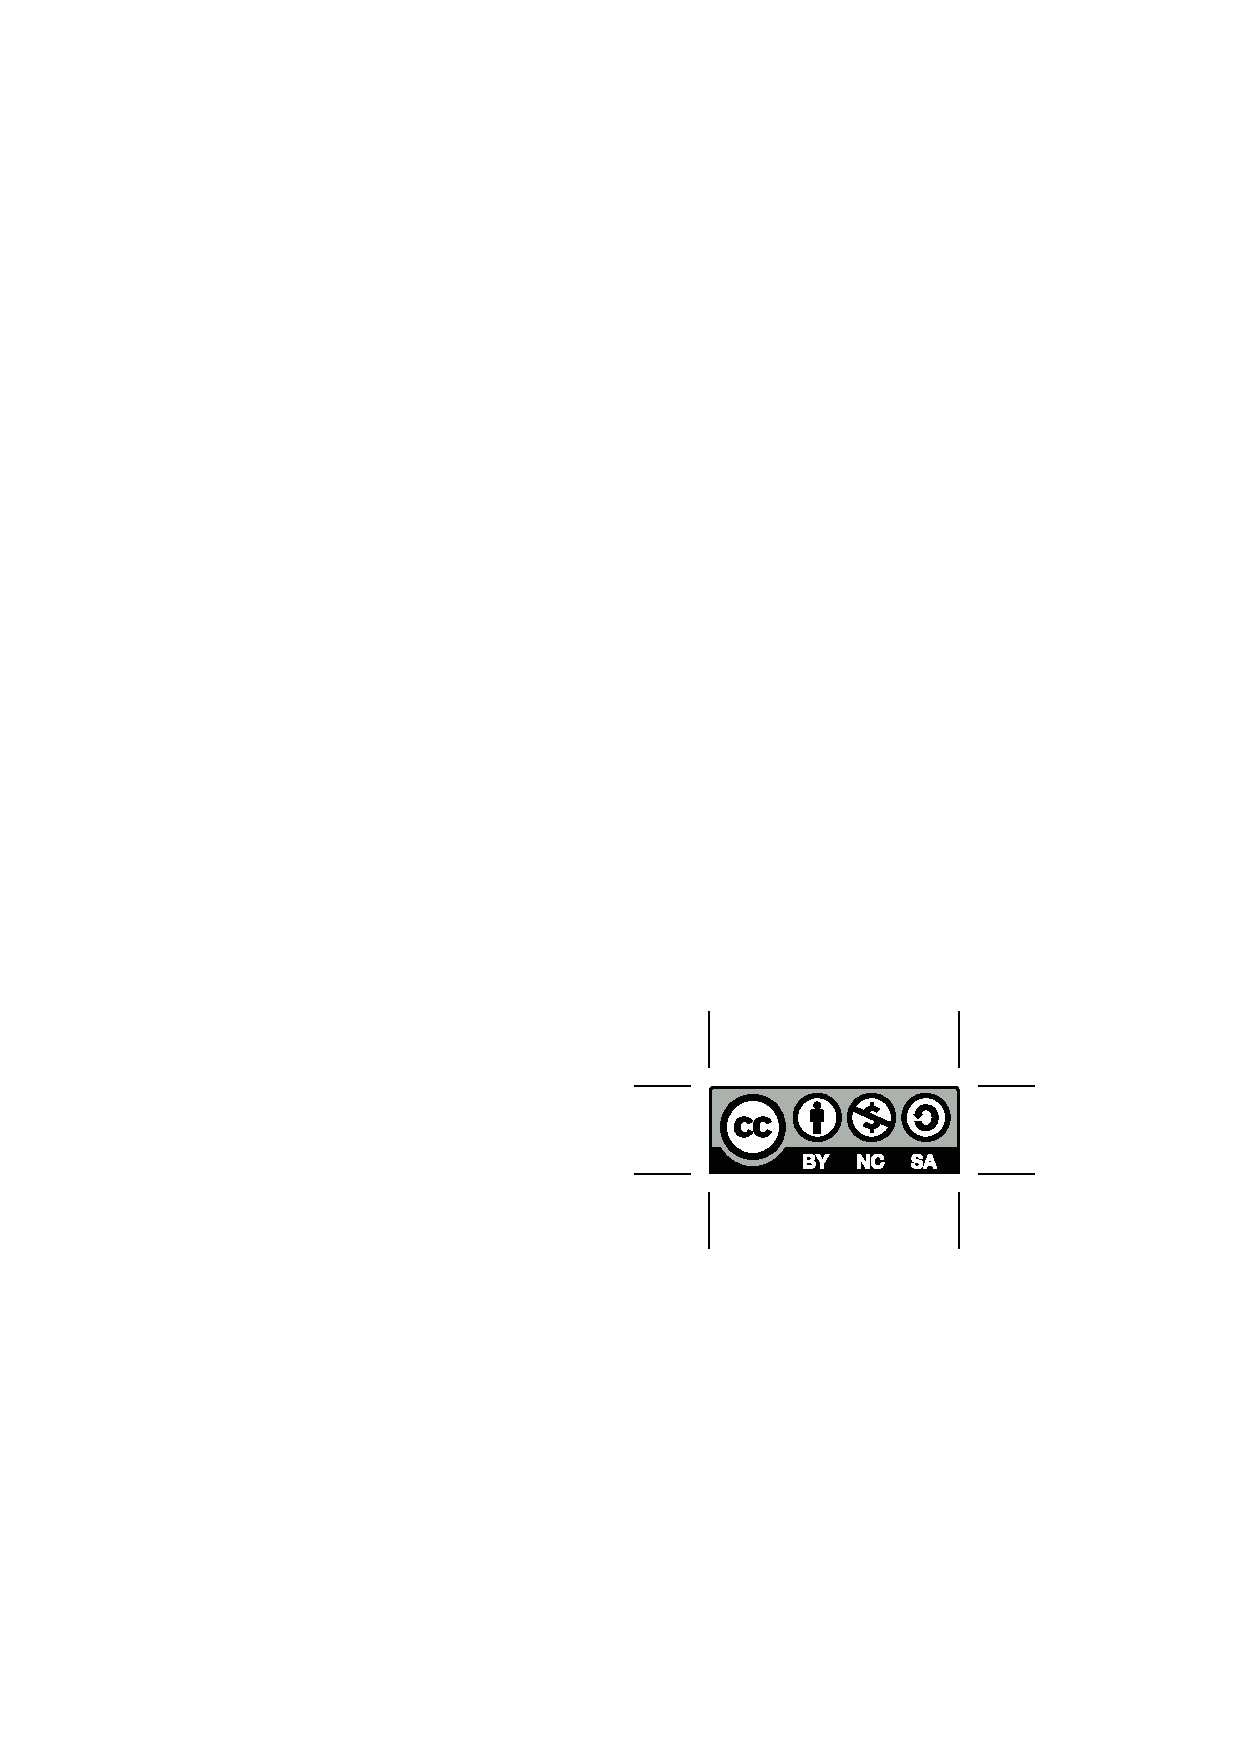
\includegraphics[width=1.38in]{license}
%\end{floatingfigure}

\bigskip

\noindent
This work is licensed under the Creative Commons
Attribution-Non\-commercial-Share Alike 3.0 United States License. To view a
copy of this license, visit
\url{http://creativecommons.org/licenses/by-nc-sa/3.0/us/} or send a letter to
Creative Commons, 171 Second Street, Suite 300, San Francisco, California,
94105, USA.
%\end{small}

\bigskip

\noindent
You can use, print, duplicate, share these notes as much as you want.  You can
base your own notes on these and reuse parts if you keep the license the
same.  If you plan to use these commercially (sell them for more than just
duplicating cost), then you need to contact me and we will work something out.
If you are printing a course pack for your students, then it is fine if the 
duplication service is charging a fee for printing and selling the printed
copy.  I consider that duplicating cost.

\bigskip

\noindent
During the writing of these notes, 
the author was in part supported by NSF grant DMS-1362337.

\bigskip

\noindent
See \url{http://www.jirka.org/ra2/} for more information
(including contact information).


% For large print do this
%\large

\microtypesetup{protrusion=false}
\tableofcontents
\microtypesetup{protrusion=true}

\newpage

%%%%%%%%%%%%%%%%%%%%%%%%%%%%%%%%%%%%%%%%%%%%%%%%%%%%%%%%%%%%%%%%%%%%%%%%%%%%%%
%%%%%%%%%%%%%%%%%%%%%%%%%%%%%%%%%%%%%%%%%%%%%%%%%%%%%%%%%%%%%%%%%%%%%%%%%%%%%%
%%%%%%%%%%%%%%%%%%%%%%%%%%%%%%%%%%%%%%%%%%%%%%%%%%%%%%%%%%%%%%%%%%%%%%%%%%%%%%

\chapter*{Introduction}
\addcontentsline{toc}{chapter}{Introduction}
\markboth{INTRODUCTION}{INTRODUCTION}

%%%%%%%%%%%%%%%%%%%%%%%%%%%%%%%%%%%%%%%%%%%%%%%%%%%%%%%%%%%%%%%%%%%%%%%%%%%%%%

\section*{About this book}

This book is the continuation of ``Basic Analysis''.  The book is meant to
be a seamless continuation, so the chapters are numbered to start where the
first volume left off.

This book is unfinished, and at this point is likely in a state of
constant flux, and will have possibly more topics added on the end (or even
in the middle).
Numbering will
change, things will get reshuffled.  Do not expect constancy, that is,
at least for now.  At
some point in the future, this book will also become stable, but until then,
you have been warned.

%%%%%%%%%%%%%%%%%%%%%%%%%%%%%%%%%%%%%%%%%%%%%%%%%%%%%%%%%%%%%%%%%%%%%%%%%%%%%%

%%%%%%%%%%%%%%%%%%%%%%%%%%%%%%%%%%%%%%%%%%%%%%%%%%%%%%%%%%%%%%%%%%%%%%%%%%%%%%
%%%%%%%%%%%%%%%%%%%%%%%%%%%%%%%%%%%%%%%%%%%%%%%%%%%%%%%%%%%%%%%%%%%%%%%%%%%%%%
%%%%%%%%%%%%%%%%%%%%%%%%%%%%%%%%%%%%%%%%%%%%%%%%%%%%%%%%%%%%%%%%%%%%%%%%%%%%%%

\chapter{Several variables and partial derivatives} \label{pd:chapter}

%\vspace*{-3in}
%{\large DRAFT~~~~DRAFT~~~~DRAFT~~~~DRAFT~~~~\today}
%\vspace*{2.508in}

%%%%%%%%%%%%%%%%%%%%%%%%%%%%%%%%%%%%%%%%%%%%%%%%%%%%%%%%%%%%%%%%%%%%%%%%%%%%%%

\section{Vector spaces, linear mappings, and convexity}
\label{sec:vectorspaces}

\sectionnotes{2--3 lectures}

\subsection{Vector spaces}

The euclidean space $\R^n$ has already made an appearance in the metric
space chapter.  In this chapter, we will extend the differential calculus
we created for one variable to several variables.  The key idea in
differential calculus is to approximate functions by lines and linear
functions.  In several variables we must introduce a little bit of linear
algebra before we can move on.  So
let us start with vector spaces and linear functions on vector spaces.

While it is common to use $\vec{x}$ or the bold
$\mathbf{x}$ for elements of $\R^n$,
especially in the applied sciences,
we use just plain $x$, which is common in mathematics.
That is, $v \in \R^n$ is a \emph{\myindex{vector}}, which means 
$v = (v_1,v_2,\ldots,v_n)$ is an $n$-tuple of
real numbers.\footnote{Subscripts are used for many purposes,
so sometimes we may have several vectors which may also
be identified by subscript such as a finite or infinite sequence of
vectors $y_1,y_2,\ldots$.}
%For example, we can have vectors $x_1$ and $x_2$
%in $\R^n$ and then $x_1 = (x_1^1,x_1^2,\ldots,x_1^n)$ and
%$x_2 = (x_2^1,x_2^2,\ldots,x_2^n)$.

It is common to write vectors as
\emph{\myindex{column vectors}}, that is, $n \times 1$ matrices:
\begin{equation*}
v =
(v_1,v_2,\ldots,v_n) =
\mbox{ \scriptsize
$\begin{bmatrix}
v_1 \\ v_2 \\ \vdots \\ v_n
\end{bmatrix}$ }.
\end{equation*}
We will do so when convenient.
%We will use this notation with square
%brackets and use round brackets for just an $n$-tuple of numbers.
We call real numbers
\emph{\myindex{scalars}} to distinguish them from vectors.

The set $\R^n$ has a so-called \emph{vector space} structure defined on it.
However,
even though we will be looking at functions defined on $\R^n$,
not all spaces we wish to deal with are equal to $\R^n$.  Therefore, let us
define the abstract notion of the vector space.

\begin{defn}
Let $X$ be a set together with
operations of addition, $+ \colon X \times X \to X$,
and multiplication, $\cdot \colon \R \times X \to X$, (we usually write $ax$ instead of $a
\cdot x$).  $X$ is called a \emph{\myindex{vector space}} (or a
\emph{\myindex{real vector space}})
if the following conditions are satisfied:
\begin{enumerate}[(i)]
\item (Addition is associative) \quad If $u, v, w \in X$, then $u+(v+w) = (u+v)+w$.
\item (Addition is commutative) \quad If $u, v \in X$, then $u+v = v+u$.
\item (Additive identity) \quad There is a $0 \in X$ such that $v+0=v$ for all $v \in X$.
\item (Additive inverse) \quad For every $v \in X$, there is a $-v \in X$,
such that $v+(-v)=0$.
\item (Distributive law) \quad If $a \in \R$, $u,v \in X$, then
$a(u+v) = au+av$.
\item (Distributive law) \quad If $a,b \in \R$, $v \in X$, then
$(a+b)v = av+bv$.
\item (Multiplication is associative) \quad If $a,b \in \R$, $v \in X$, then
$(ab)v = a(bv)$.
\item (Multiplicative identity) \quad $1v = v$ for all $v \in X$.
\end{enumerate}
Elements of a vector space are usually called \emph{vectors}\index{vector},
even if they
are not elements of $\R^n$ (vectors in the ``traditional'' sense).

If $Y \subset X$ is a subset that is a vector space itself with the same
operations, then $Y$ is called a \emph{\myindex{subspace}} or
\emph{\myindex{vector subspace}} of $X$.
\end{defn}

%In short $X$ is an Abelian group with respect to the addition, and equipped
%with multiplication by scalars.

\begin{example}
An example vector space is $\R^n$, where addition
and multiplication by a constant is done componentwise:
if $a \in \R$, $v = (v_1,v_2,\ldots,v_n) \in \R^n$, and $w =
(w_1,w_2,\ldots,w_n) \in \R^n$, then
\begin{align*}
& v+w :=
(v_1,v_2,\ldots,v_n) +
(w_1,w_2,\ldots,w_n) 
=
(v_1+w_1,v_2+w_2,\ldots,v_n+w_n) , \\
& a v :=
a (v_1,v_2,\ldots,v_n) =
(a v_1, a v_2,\ldots, a v_n) .
\end{align*}
\end{example}

In this book we mostly deal with vector spaces that can be often regarded as
subsets of $\R^n$, but there are other vector spaces useful in
analysis.  Let us give a couple of examples.

\begin{example}
A trivial example of a vector space (the smallest one in fact) is just
$X = \{ 0 \}$.  The operations are defined in the obvious way.  You always
need a zero vector to exist, so all vector spaces are nonempty sets.
\end{example}

\begin{example}
The space $C([0,1],\R)$ of continuous functions on the interval $[0,1]$
is a vector space.  For two functions $f$ and $g$ in $C([0,1],\R)$ and
$a \in \R$ we make the obvious definitions of $f+g$ and $af$:
\begin{equation*}
(f+g)(x) := f(x) + g(x), \qquad (af) (x) := a\bigl(f(x)\bigr) .
\end{equation*}
The 0 is the function that is identically zero.  We leave it as an exercise
to check that all the vector space conditions are satisfied.
\end{example}

\begin{example}
The space of polynomials $c_0 + c_1 t + c_2 t^2 + \cdots + c_m t^m$
is a vector space, let us denote it by $\R[t]$ (coefficients are real and
the variable is $t$).  The operations can be defined in the same way as for
functions above.
Suppose we have
two polynomials, one of degree $m$ and one of degree $n$.  Assume $n
\geq m$ for simplicity.  Then
\begin{multline*}
(c_0 + c_1 t + c_2 t^2 + \cdots + c_m t^m)
+
(d_0 + d_1 t + d_2 t^2 + \cdots + d_n t^n)
= \\
(c_0+d_0) + (c_1+d_1) t + (c_2 + d_2) t^2 + \cdots + (c_m+d_m) t^m
+ d_{m+1} t^{m+1} + \cdots + d_n t^n
\end{multline*}
and
\begin{equation*}
a(c_0 + c_1 t + c_2 t^2 + \cdots + c_m t^m)
=
(ac_0) + (ac_1) t + (ac_2) t^2 + \cdots + (ac_m) t^m  .
\end{equation*}
Despite what it looks like, $\R[t]$ is not equivalent to $\R^n$ for any $n$.  In
particular it is not ``finite dimensional'', we will make this notion
precise in just a little bit.  One can make a finite
dimensional vector subspace by restricting the degree.  For example,
if we say $\sP_n$ is the space of polynomials of degree $n$ or less,
then we have a finite dimensional vector space.

The space $\R[t]$ can be thought of as a subspace of $C(\R,\R)$.  If we
restrict the range of $t$ to $[0,1]$, $\R[t]$ can be identified with
a subspace of $C([0,1],\R)$.
\end{example}

It is often better to think of even simpler ``finite dimensional''
vector spaces using the abstract notion rather than always $\R^n$.
It is possible to use other fields than $\R$ in the definition (for
example it is common to use the complex numbers $\C$), but let us stick with
the real numbers\footnote{If you want a very funky vector space over a different field,
$\R$ itself is a vector space over the rational numbers.}.

\subsection{Linear combinations and dimension}

\begin{defn}
Suppose $X$ is a vector space,
$x_1, x_2, \ldots, x_k \in X$ are vectors, and
$a_1, a_2, \ldots, a_k \in \R$ are scalars.  Then
\begin{equation*}
a_1 x_1 + 
a_2 x_2 +  \cdots
+ a_k x_k
\end{equation*}
is called a \emph{\myindex{linear combination}} of the vectors $x_1, x_2,
\ldots, x_k$.

%Note that if $x_1, \ldots, x_k$ are in a vector space $X$, then
%any linear combination of $x_1, \ldots, x_k$ is also in $X$.

If $Y \subset X$ is a set then the \emph{\myindex{span}} of $Y$, or in notation
$\spn(Y)$, is the set of all linear combinations
of some finite number of elements of $Y$.  We also
say $Y$ \emph{\myindex{spans}} $\spn(Y)$.
\end{defn}

\begin{example}
Let $Y := \{ (1,1) \} \subset \R^2$.  Then
\begin{equation*}
\spn(Y)
=
\{ (x,x) \in \R^2 : x \in \R \} .
\end{equation*}
That is, $\spn(Y)$ is the line through the origin and the point $(1,1)$.
\end{example}

\begin{example} \label{example:vecspr2span}
Let $Y := \{ (1,1), (0,1) \} \subset \R^2$.  Then
\begin{equation*}
\spn(Y)
=
\R^2 ,
\end{equation*}
as any point $(x,y) \in \R^2$ can be written as
a linear combination
\begin{equation*}
(x,y) = x (1,1) + (y-x) (0,1) .
\end{equation*}
\end{example}

A sum of two linear combinations is again a linear combination, and
a scalar multiple of a linear combination is a linear combination,
which proves the following proposition.

\begin{prop}
Let $X$ be a vector space.  For any $Y \subset X$,
the set $\spn(Y)$ is a vector space itself.
That is, $\spn(Y)$ is a subspace of $X$.
\end{prop}

If $Y$ is already a vector space then $\spn(Y) = Y$.

\begin{defn}
A set of vectors $\{ x_1, x_2, \ldots, x_k \} \subset X$ is 
\emph{\myindex{linearly independent}}, if the only solution to
\begin{equation} \label{eq:lincomb}
a_1 x_1 + a_2 x_2 + \cdots + a_k x_k = 0
\end{equation}
is the trivial solution $a_1 = a_2 = \cdots = a_k = 0$.
%Here 0 is the vector of all zeros.
A set that is not linearly independent, is
\emph{\myindex{linearly dependent}}.

A linearly independent set $B$ of vectors such that
$\spn(B) = X$ 
is called a \emph{\myindex{basis}} of $X$.  For example the
set $Y$ of the two vectors in
\exampleref{example:vecspr2span} is a basis of $\R^2$.

If a vector space $X$ contains a linearly independent set of $d$ vectors,
but no linearly independent set of $d+1$ vectors then we say
the \emph{\myindex{dimension}} or $\dim \, X := d$.  If for all $d \in \N$ the vector space
$X$ contains a set of $d$ linearly independent vectors, we say
$X$ is infinite dimensional and write $\dim \, X := \infty$.
\end{defn}

Clearly for the trivial vector space, $\dim \, \{ 0 \} = 0$.
%So far we have not shown that any other vector space has a finite dimension.
We will see in a moment that any vector space that is a subset of $\R^n$
has a finite dimension, and that dimension is less than or equal to $n$.

If a set is linearly dependent, then one of the
vectors is a linear combination of the others.  In other words, in
\eqref{eq:lincomb}
if $a_j \not= 0$, then we can solve for $x_j$
\begin{equation*}
x_j = \frac{a_1}{a_j} x_1 + \cdots + 
\frac{a_{j-1}}{a_j} x_{j-1} +
\frac{a_{j+1}}{a_j} x_{j+1} +
\cdots + 
\frac{a_k}{a_k} x_k .
\end{equation*}
Clearly then the vector $x_j$ has at least two different representations
as linear combinations of $\{ x_1,x_2,\ldots,x_k \}$.  

\begin{prop}
If $B = \{ x_1, x_2, \ldots, x_k \}$ is a basis of a vector space $X$, then
every point $y \in X$ has a unique representation of the form
\begin{equation*}
y = \sum_{j=1}^k a_j x_j
\end{equation*}
for some scalars $a_1, a_2, \ldots, a_k$.
\end{prop}

\begin{proof}
Every $y \in X$ is a linear combination of elements of $B$
since $X$ is the span of $B$.  For uniqueness
suppose
\begin{equation*}
y = \sum_{j=1}^k a_j x_j = \sum_{j=1}^k b_j x_j ,
\end{equation*}
then
\begin{equation*}
\sum_{j=1}^k (a_j-b_j) x_j = 0 .
\end{equation*}
By linear independence of the basis $a_j = b_j$ for all $j$.
\end{proof}

For $\R^n$
we define
\begin{equation*}
e_1 := (1,0,0,\ldots,0) , \quad
e_2 := (0,1,0,\ldots,0) , \quad \ldots, \quad
e_n := (0,0,0,\ldots,1) ,
\end{equation*}
and call this the \emph{\myindex{standard basis}} of $\R^n$.
We use the same letters $e_j$ for any $\R^n$, and
which space $\R^n$ we are working in is understood from context.
A direct computation shows that $\{ e_1, e_2, \ldots, e_n \}$ is really
a basis of $\R^n$; it spans $\R^n$ and is
linearly independent.  In fact,
\begin{equation*}
x = (x_1,x_2,\ldots,x_n) = \sum_{j=1}^n x_j e_j .
\end{equation*}

\begin{prop} \label{mv:dimprop}
%(\textbf{(Theorems 9.2 and 9.3 in Rudin):})
Let $X$ be a vector space and $d$ a nonnegative integer.
\begin{enumerate}[(i)]
\item \label{mv:dimprop:i}
If $X$ is spanned by $d$ vectors, then $\dim \, X \leq d$.
\item \label{mv:dimprop:ii}
$\dim \, X = d$ if and only if $X$ has a basis of $d$
vectors (and so every basis has $d$ vectors).
\item \label{mv:dimprop:iii}
In particular, $\dim \, \R^n = n$.
\item \label{mv:dimprop:iv}
If $Y \subset X$ is a vector subspace and $\dim \, X = d$,
then $\dim \, Y \leq d$.
\item \label{mv:dimprop:v}
If $\dim \, X = d$ and a set $T$ of $d$ vectors spans $X$,
then $T$ is linearly independent.
\item \label{mv:dimprop:vi}
If $\dim \, X = d$ and a set $T$ of $m$ vectors is
linearly independent, then there is a set $S$ of $d-m$
vectors such that $T \cup S$ is a basis of $X$.
\end{enumerate}
\end{prop}

\begin{proof}
Let us start with \ref{mv:dimprop:i}.
Suppose $S = \{ x_1 , x_2, \ldots, x_d \}$ spans $X$, and
$T = \{ y_1, y_2, \ldots, y_m \}$ is a set of linearly independent
vectors of $X$.  We wish to show that $m \leq d$.
Write
\begin{equation*}
y_1 = \sum_{k=1}^d a_{k,1} x_k ,
\end{equation*}
for some numbers $a_{1,1},a_{2,1},\ldots,a_{d,1}$,
which we can do as $S$ spans $X$.  One of the
$a_{k,1}$ is nonzero (otherwise $y_1$ would be zero),
so suppose without loss of generality that this
is $a_{1,1}$.  Then we can solve
\begin{equation*}
x_1 = \frac{1}{a_{1,1}} y_1 - \sum_{k=2}^d \frac{a_{k,1}}{a_{1,1}} x_k .
\end{equation*}
In particular $\{ y_1 , x_2, \ldots, x_d \}$ span $X$, since $x_1$ can be
obtained from $\{ y_1 , x_2, \ldots, x_d \}$.  Therefore, there are some numbers
for some numbers $a_{1,2},a_{2,2},\ldots,a_{d,2}$, such that
\begin{equation*}
y_2 = a_{1,2} y_1 + \sum_{k=2}^d a_{k,2} x_k .
\end{equation*}
As $T$ is linearly independent, we must have that one of the $a_{k,2}$
for $k \geq 2$ must be nonzero.  Without loss of generality suppose 
$a_{2,2} \not= 0$.  Proceed to solve for 
\begin{equation*}
x_2 = \frac{1}{a_{2,2}} y_2 - \frac{a_{1,2}}{a_{2,2}} y_1 - \sum_{k=3}^d
\frac{a_{k,2}}{a_{2,2}} x_k .
\end{equation*}
In particular 
$\{ y_1 , y_2, x_3, \ldots, x_d \}$ spans $X$.
%The astute reader will think back to linear algebra and notice that we are
%row-reducing a matrix.

We continue this procedure.  If $m < d$, then we are done.  So suppose
$m \geq d$.
After $d$ steps we obtain that 
$\{ y_1 , y_2, \ldots, y_d \}$ spans $X$.  Any
other vector $v$ in $X$ is a linear combination of
$\{ y_1 , y_2, \ldots, y_d \}$, and hence cannot be in $T$ as $T$ is
linearly independent.  So $m = d$.

Let us look at \ref{mv:dimprop:ii}.
First notice that if we have a set $T$ of $k$ linearly independent vectors
that do not span $X$, then we can always choose a vector $v \in X \setminus
\spn (T)$.  The set $T \cup \{ v \}$ is linearly independent (exercise).
If $\dim \, X = d$,
then there must exist some linearly independent set of $d$ vectors $T$,
and it must span $X$, otherwise we could choose a larger set of linearly
independent vectors.  So we have a basis of $d$ vectors.
On the other hand if we have a basis of $d$ vectors,
it is linearly independent and spans $X$.  By \ref{mv:dimprop:i} we know
there is no set of $d+1$ linearly independent vectors, so dimension must be $d$.

For \ref{mv:dimprop:iii} notice that $\{ e_1, e_2, \ldots, e_n \}$ is a basis of $\R^n$.

To see \ref{mv:dimprop:iv},
suppose $Y$ is a vector space and $Y \subset X$,
where $\dim \, X = d$.  As $X$ cannot contain $d+1$ linearly independent
vectors, neither can $Y$.

For \ref{mv:dimprop:v} suppose $T$ is a set of $m$ vectors that is linearly dependent
and spans $X$.  Then one of the
vectors is a linear combination of the others.  Therefore if we remove it
from $T$ we obtain a set of $m-1$ vectors that still span $X$ and hence
$\dim \, X \leq m-1$ by \ref{mv:dimprop:i}.

For \ref{mv:dimprop:vi} suppose $T = \{ x_1, x_2, \ldots, x_m \}$ is
a linearly independent set.  We follow the procedure above in the proof of
\ref{mv:dimprop:ii}
to keep adding vectors while keeping the set linearly independent.
As the dimension is $d$ we can add a vector exactly $d-m$ times.
\end{proof}

\subsection{Linear mappings}

A function $f \colon X \to Y$, when $Y$ is not $\R$, is often called a
\emph{\myindex{mapping}} or a \emph{\myindex{map}}
rather than a \emph{function}.
%  The word
%function is then usually reserved for the case $Y=\R$.


\begin{defn}
A mapping $A \colon X \to Y$ of vector spaces $X$ and $Y$
is \emph{\myindex{linear}} (or a
\emph{\myindex{linear transformation}})
if for every $a \in \R$ and $x,y \in X$
we have
\begin{equation*}
A(a x) = a A(x), \qquad \text{and} \qquad A(x+y) = A(x)+A(y) .
\end{equation*}
We usually write $Ax$ instead of $A(x)$ if $A$ is linear.

If $A$ is one-to-one an onto then we say $A$ is
\emph{invertible}\index{invertible linear transformation}
and we denote the inverse by $A^{-1}$.

If $A \colon X \to X$ is linear then we say $A$ is a
\emph{\myindex{linear operator}} on $X$.

We write $L(X,Y)$ for the set of all linear transformations from $X$ to
$Y$, and just $L(X)$ for the set of linear operators on $X$.
If $a \in \R$ and $A,B \in L(X,Y)$, define
the transformations $aA$ and $A+B$ by
\begin{equation*}
(aA)(x) := aAx ,
\qquad
(A+B)(x) := Ax + Bx .
\end{equation*}

If $A \in L(Y,Z)$ and $B \in L(X,Y)$, define the
transformation $AB$ as the composition $A \circ B$, that is,
\begin{equation*}
ABx := A(Bx) .
\end{equation*}

Finally denote by $I \in L(X)$ the \emph{\myindex{identity}}: 
the linear operator such that $Ix = x$ for all $x$.
\end{defn}

It is not hard to see that $aA \in L(X,Y)$
and $A+B \in L(X,Y)$, and that $AB \in L(X,Z)$.
In particular, $L(X,Y)$ is a vector space.
As the set $L(X)$ is not only a vector space, but also
admits a product, it is often called an \emph{\myindex{algebra}}.

An immediate consequence of the definition of a linear mapping is that if
$A$ is linear then $A0 = 0$.

\begin{prop}
If $A \in L(X,Y)$ is invertible, then $A^{-1}$ is linear.
\end{prop}

\begin{proof}
Let $a \in \R$ and $y \in Y$.  As $A$ is onto, then there is an 
$x$ such that $y = Ax$, and further as it is also one-to-one
$A^{-1}(Az) = z$ for all $z \in X$.  So
\begin{equation*}
A^{-1}(ay)
=
A^{-1}(aAx)
=
A^{-1}\bigl(A(ax)\bigr)
= ax
= aA^{-1}(y).
\end{equation*}
Similarly let $y_1,y_2 \in Y$, and $x_1, x_2 \in X$ such that
$Ax_1 = y_1$ and 
$Ax_2 = y_2$, then
\begin{equation*}
A^{-1}(y_1+y_2)
=
A^{-1}(Ax_1+Ax_2)
=
A^{-1}\bigl(A(x_1+x_2)\bigr)
= x_1+x_2
= A^{-1}(y_1) + A^{-1}(y_2). \qedhere
\end{equation*}
\end{proof}

\begin{prop} \label{mv:lindefonbasis}
If $A \in L(X,Y)$ is linear then it is completely determined
by its values on a basis of $X$.
Furthermore, if $B$ is a basis of $X$,
then any function $\widetilde{A} \colon B \to Y$ extends to a linear
function on $X$.
\end{prop}

We will only prove this proposition for finite dimensional spaces, as we do
not need infinite dimensional spaces.
For infinite dimensional spaces, the proof is essentially the same, but a
little trickier to write, so let us stick with finitely many dimensions.

\begin{proof}
Let $\{ x_1, x_2, \ldots, x_n \}$ be a basis and suppose 
$A x_j = y_j$.  Every $x \in X$ has a unique representation
\begin{equation*}
x = \sum_{j=1}^n b_j x_j
\end{equation*}
for some numbers $b_1,b_2,\ldots,b_n$.  By linearity
\begin{equation*}
Ax = 
A\sum_{j=1}^n b_j x_j
=
\sum_{j=1}^n b_j Ax_j
=
\sum_{j=1}^n b_j y_j .
\end{equation*}
The ``furthermore'' follows by setting $y_j := \widetilde{A}(x_j)$,
and defining the extension as
$Ax := \sum_{j=1}^n b_j y_j$.  The function is well defined by
uniqueness of the representation of $x$.
We leave it to the reader to check that $A$ is linear.
\end{proof}

The next proposition only works for finite dimensional vector spaces.
It is a special case of the so called rank-nullity theorem from linear
algebra.

%\textbf{Theorem 9.5:}
\begin{prop} \label{mv:prop:lin11onto}
If $X$ is a finite dimensional vector space and $A \in L(X)$, then $A$ is one-to-one if and only if it is onto.
\end{prop}

\begin{proof}
Let $\{ x_1,x_2,\ldots,x_n \}$ be a basis for $X$.
Suppose $A$ is one-to-one.  Now suppose
\begin{equation*}
\sum_{j=1}^n c_j Ax_j =
A\sum_{j=1}^n c_j x_j =
0 .
\end{equation*}
As $A$ is one-to-one,
the only vector that is taken to 0 is 0 itself.  
Hence,
\begin{equation*}
0 =
\sum_{j=1}^n c_j x_j
\end{equation*}
and $c_j = 0$ for all $j$.
So $\{ Ax_1, Ax_2, \ldots, Ax_n \}$ is a linearly independent set.
By \propref{mv:dimprop}
and the fact that the dimension is $n$, we have that
$\{ Ax_1, Ax_2, \ldots, Ax_n \}$ span $X$.  Any point $x \in X$
can be written as
\begin{equation*}
x = \sum_{j=1}^n a_j Ax_j =
A\sum_{j=1}^n a_j x_j ,
\end{equation*}
so $A$ is onto.

Now suppose $A$ is onto.  As $A$ is determined by the action on
the basis we see that every element of $X$ has to be in the span of
$\{ Ax_1, Ax_2, \ldots, Ax_n \}$.  Suppose 
\begin{equation*}
A\sum_{j=1}^n c_j x_j =
\sum_{j=1}^n c_j Ax_j = 0 .
\end{equation*}
By \propref{mv:dimprop}
$\{ Ax_1, Ax_2, \ldots, Ax_n \}$ span $X$, the set is independent,
and hence $c_j = 0$ for all $j$.  In other words if $Ax = 0$, then $x=0$.  This means that
$A$ is one-to-one:  If $Ax = Ay$, then $A(x-y) = 0$ and so
$x=y$.
\end{proof}

We leave the proof of the next proposition as an exercise.

\begin{prop} \label{prop:LXYfinitedim}
If $X$ and $Y$ are finite dimensional vector spaces, then $L(X,Y)$
is also finite dimensional.
\end{prop}

\subsection{Convexity}

A subset $U$ of a vector space is \emph{\myindex{convex}}
if whenever $x,y \in U$, the line segment from
$x$ to $y$ lies in $U$.  That is, if the \emph{\myindex{convex combination}}
$(1-t)x+ty$ is in $U$ for all $t \in [0,1]$.  See \figureref{mv:convexcomb}.

\begin{figure}[h!t]
\begin{center}
\input convexset.pdf_t
\caption{Convexity.\label{mv:convexcomb}}
\end{center}
\end{figure}

Note that in $\R$, every connected interval is convex.  In $\R^2$ (or higher
dimensions) there are lots of nonconvex connected sets.  For example
the set $\R^2 \setminus \{0\}$ is not convex but it is connected.  To see
this simply take any $x \in \R^2 \setminus \{0\}$ and let $y:=-x$.
Then $(\nicefrac{1}{2})x + (\nicefrac{1}{2})y = 0$, which is not in the set.
On the other hand, the ball $B(x,r) \subset \R^n$ (using the standard metric
on $\R^n$)
is always convex by the triangle inequality.

\begin{exercise}
Show that in $\R^n$ any ball $B(x,r)$ for $x \in \R^n$ and $r > 0$ is
convex.
\end{exercise}

\begin{example}
Any subspace $V$ of a vector space $X$ is convex.
\end{example}

\begin{example}
A somewhat more complicated example is given by the following.  Let
$C([0,1],\R)$ be the vector space of continuous real valued functions on $\R$.
Let $X \subset C([0,1],\R)$ be the set of those $f$ such  
\begin{equation*}
\int_0^1 f(x)~dx \leq 1 \qquad \text{and} \qquad
f(x) \geq 0 \text{ for all $x \in [0,1]$} .
\end{equation*}
Then $X$ is convex.  Take $t \in [0,1]$ and note that if $f,g \in X$
then $t f(x) + (1-t) g(x) \geq 0$ for all $x$.  Furthermore
\begin{equation*}
\int_0^1 \bigl(tf(x) + (1-t)g(x)\bigr) ~dx
=
t \int_0^1 f(x) ~dx
+ (1-t)\int_0^1 g(x) ~dx \leq 1 .
\end{equation*}
Note that $X$ is not a subspace of $C([0,1],\R)$.
\end{example}

\begin{prop}
The intersection two convex sets is convex.  In fact,
if $\{ C_\lambda \}_{\lambda \in I}$ is
an arbitrary collection of convex sets, then
\begin{equation*}
C := \bigcap_{\lambda \in I} C_\lambda
\end{equation*}
is convex.
\end{prop}

\begin{proof}
The proof is easy.  If $x, y \in C$, then $x,y \in C_\lambda$ for all
$\lambda \in I$, and hence if $t \in [0,1]$, then $tx + (1-t)y \in
C_\lambda$ for all $\lambda \in I$.  Therefore $tx + (1-t)y \in C$ and $C$
is convex.
\end{proof}

\begin{prop}
Let $T \colon V \to W$ be a linear mapping between two vector spaces and
let $C \subset V$ be a convex set.  Then $T(C)$ is convex.
\end{prop}

\begin{proof}
Take any two points $p,q \in T(C)$.  Pick $x,y \in C$ such that
$Tx = p$ and $Ty=q$.  As $C$ is convex then for all $t \in [0,1]$
we have $tx+(1-t)y \in C$, so
\begin{equation*}
tp+(1-t)q 
=
tTx+(1-t)Ty
=
T\bigl(tx+(1-t)y\bigr)
\in T(C) .  \qedhere
\end{equation*}
\end{proof}

For completeness, a very useful construction is the
\emph{\myindex{convex hull}}.  Given any set $S \subset V$ of a vector
space, define the convex hull of $S$, by
\begin{equation*}
\operatorname{co}(S) :=
\bigcap \{ C \subset V : S \subset C, \text{ and $C$ is convex} \} .
\end{equation*}
That is, the convex hull is the smallest convex set containing $S$.  
By a proposition above, the intersection of convex sets is convex and
hence, the convex hull is convex.

\begin{example}
The convex hull of 0 and 1 in $\R$ is $[0,1]$.  Proof:
Any convex set containing 0 and 1 must contain $[0,1]$.  The set $[0,1]$
is convex, therefore it must be the convex hull.
\end{example}

\subsection{Exercises}

\begin{exercise}
Verify that $\R^n$ is a vector space.
\end{exercise}

\begin{exercise}
Let $X$ be a vector space.
Prove that a finite set of vectors $\{ x_1,\ldots,x_n \} \subset X$ 
is linearly independent if and only if for every $j=1,2,\ldots,n$
\begin{equation*}
\spn( \{ x_1,\ldots,x_{j-1},x_{j+1},\ldots,x_n \}) \subsetneq
\spn( \{ x_1,\ldots,x_n \}) .
\end{equation*}
That is, the span of the set with one vector removed is strictly smaller.
\end{exercise}

\begin{exercise}[Challenging]
Prove that $C([0,1],\R)$ is an infinite dimensional vector space
where the operations are defined in the obvious way:
$s=f+g$ and $m=fg$ are defined as
$s(x) := f(x)+g(x)$ and
$m(x) := f(x)g(x)$.
Hint: for the dimension, think of functions that are only nonzero
on the interval $(\nicefrac{1}{n+1},\nicefrac{1}{n})$.
\end{exercise}

\begin{exercise}
Let $k \colon [0,1]^2 \to \R$ be continuous.  Show that
$L \colon C([0,1],\R) \to C([0,1],\R)$ defined by
\begin{equation*}
Lf(y) := \int_0^1 k(x,y)f(x)~dx
\end{equation*}
is a linear operator.  That is, show that $L$ is well defined (that
$Lf$ is continuous), and that $L$ is linear.
\end{exercise}

\begin{exercise}
Let $\sP_n$ be the vector space of polynomials in one variable of degree $n$
or less.  Show that $\sP_n$ is a vector space of dimension $n+1$.
\end{exercise}

\begin{exercise}
Let $\R[t]$ be the vector space of polynomials in one variable $t$.  Let
$D \colon \R[t] \to \R[t]$ be the derivative operator (derivative in $t$).
Show that $D$ is a linear operator.
\end{exercise}

\begin{exercise}
Let us show that \propref{mv:prop:lin11onto} only works in finite
dimensions.  Take $\R[t]$ and define the operator $A \colon \R[t] \to \R[t]$
by $A\bigl(P(t)\bigr) = tP(t)$.  Show that $A$ is linear and one-to-one, but
show that it is not onto.
\end{exercise}

\begin{exercise}
Finish the proof of \propref{mv:lindefonbasis} in finite dimensional case.
That is, suppose,
$\{ x_1, x_2,\ldots x_n \}$ is a basis of $X$,
$\{ y_1, y_2,\ldots y_n \} \subset Y$ and we define a
function
\begin{equation*}
Ax := \sum_{j=1}^n b_j y_j, \qquad \text{if} \quad x=\sum_{j=1}^n b_j x_j .
\end{equation*}
Then prove that $A \colon X \to Y$ is linear.
\end{exercise}


\begin{exercise}
Prove \propref{prop:LXYfinitedim}.  Hint: A linear operator is determined by
its action on a basis.  So given two bases
$\{ x_1,\ldots,x_n \}$ and
$\{ y_1,\ldots,y_m \}$ for $X$ and $Y$ respectively, consider the linear
operators $A_{jk}$ that send $A_{jk} x_j = y_k$, and 
$A_{jk} x_\ell = 0$ if $\ell \not= j$.
\end{exercise}

\begin{exercise}[Easy]
Suppose $X$ and $Y$ are vector spaces and $A \in L(X,Y)$ is a linear
operator.\\
a) Show that the nullspace $N := \{ x \in X : Ax = 0 \}$ is a
vectorspace.
\\
b) Show that the range $R := \{ y \in Y : Ax = y \text{ for some $x \in X$} \}$ is a
vectorspace.
\end{exercise}

\begin{exercise}[Easy]
Show by example that a union of convex sets need not be convex.
\end{exercise}

\begin{exercise}
Compute the convex hull of the set of 3 points $\{ (0,0), (0,1), (1,1) \}$ in
$\R^2$.
\end{exercise}

\begin{exercise}
Show that the set $\{ (x,y) \in \R^2 : y > x^2 \}$ is a convex set.
\end{exercise}

\begin{exercise}
Show that every convex set in $\R^n$ is connected using the standard
topology on $\R^n$.
\end{exercise}

\begin{exercise}
Suppose $K \subset \R^2$ is a convex set such that the only point of
the form $(x,0)$ in $K$ is the point $(0,0)$.  Further suppose that
there $(0,1) \in K$ and $(1,1) \in K$.  Then show that if $(x,y) \in K$
then $y > 0$ unless $x=0$.
\end{exercise}

%FIXME

%%%%%%%%%%%%%%%%%%%%%%%%%%%%%%%%%%%%%%%%%%%%%%%%%%%%%%%%%%%%%%%%%%%%%%%%%%%%%%

\sectionnewpage
%\section{Norms, matrices, and determinants}
\section{Analysis with vector spaces}
\label{sec:normsmatsdets}

\sectionnotes{??? lectures}

\subsection{Norms}

Let us start measuring distance.

\begin{defn}
If $X$ is a vector space, then we say
a function $\snorm{\cdot} \colon X \to \R$ is a \emph{\myindex{norm}} if:
\begin{enumerate}[(i)]
\item \label{defn:norm:i} $\snorm{x} \geq 0$, with $\snorm{x}=0$ if and only if $x=0$.
\item \label{defn:norm:ii} $\snorm{cx} = \abs{c}\snorm{x}$ for all $c \in \R$ and $x \in X$.
\item \label{defn:norm:iii} $\snorm{x+y} \leq \snorm{x}+\snorm{y}$ for all $x,y \in X$
\qquad (Triangle inequality)\index{triangle inequality for norms}.
\end{enumerate}
\end{defn}

Before defining the standard norm on $\R^n$, let us
define the standard 
scalar \emph{\myindex{dot product}} on $\R^n$.  For two vectors
if $x=(x_1,x_2,\ldots,x_n) \in \R^n$
and $y=(y_1,y_2,\ldots,y_n) \in \R^n$, define
\begin{equation*}
x \cdot y := \sum_{j=1}^n x_j y_j .
\end{equation*}
It is easy to see that the dot product is linear in each variable
separately, that is, it is a linear mapping when you keep one of the
variables constant.
The \emph{\myindex{Euclidean norm}} is then defined as
\begin{equation*}
\snorm{x} := \sqrt{x \cdot x} = \sqrt{(x_1)^2+(x_2)^2 + \cdots + (x_n)^2}.
\end{equation*}
It is easy to see that the Euclidean norm satisfies \ref{defn:norm:i} and
\ref{defn:norm:ii}.  To prove
that \ref{defn:norm:iii} holds, the key
key inequality in the so-called Cauchy-Schwarz inequality that
we have seen before.  As this inequality is so important let us restate and
reprove it using the notation of this chapter.

\begin{thm}[\myindex{Cauchy-Schwarz inequality}]
Let $x, y \in \R^n$, then
\begin{equation*}
\abs{x \cdot y} \leq \snorm{x}\snorm{y} = \sqrt{x\cdot x}\, \sqrt{y\cdot y},
\end{equation*}
with equality if and only if the vectors are scalar multiples of each other.
\end{thm}

\begin{proof}
If $x=0$ or $y = 0$, then the theorem holds trivially.
So assume $x\not= 0$ and $y \not= 0$.

If $x$ is a scalar multiple of $y$, that is $x = \lambda y$ for some
$\lambda \in \R$, then the theorem holds with equality:
\begin{equation*}
\abs{\lambda y \cdot y} = \abs{\lambda} \, \abs{y\cdot y} =
\abs{\lambda} \, \snorm{y}^2 = \snorm{\lambda y} \snorm{y} .
\end{equation*}

Next take $x+ty$,
\begin{equation*}
\snorm{x+ty}^2 =
(x+ty) \cdot (x+ty) =
x \cdot x + x \cdot ty + ty \cdot x + ty \cdot ty
=
\snorm{x}^2 + 2t(x \cdot y) + t^2 \snorm{y}^2 .
\end{equation*}
If $x$ is not a scalar multiple of $y$, then 
$\snorm{x+ty}^2 > 0$ for all $t$.  So the above polynomial in $t$
is never zero.
From elementary algebra it follows that the discriminant must be negative:
\begin{equation*}
4 {(x \cdot y)}^2 - 4 \snorm{x}^2\snorm{y}^2 < 0,
\end{equation*}
or in other words ${(x \cdot y)}^2 < \snorm{x}^2\snorm{y}^2$.
\end{proof}

Item \ref{defn:norm:iii}, the triangle inequality, follows via a simple computation:
\begin{equation*}
\snorm{x+y}^2 
=
x \cdot x + y \cdot y + 2 (x \cdot y)
\leq
\snorm{x}^2 + \snorm{y}^2 + 2 (\snorm{x}+\snorm{y})
=
{(\snorm{x} + \snorm{y})}^2 .
\end{equation*}

The distance
$d(x,y) := \snorm{x-y}$ is the standard
distance function on $\R^n$ that we used when we talked about metric spaces.

In fact, on any vector space $X$, once we
have a norm (any norm),
we define a distance $d(x,y) := \snorm{x-y}$ that makes $X$ into
a metric space (an easy exercise).

%Let $A \in L(\R^n,\R^m)$.  Define
\begin{defn}
Let $A \in L(X,Y)$.  Define
\begin{equation*}
\snorm{A} :=
\sup \{ \snorm{Ax} : x \in X ~ \text{with} ~ \snorm{x} = 1 \} .
\end{equation*}
The number $\snorm{A}$ is called the \emph{\myindex{operator norm}}.  We will see below
that indeed it is a norm (at least for finite dimensional spaces).
\end{defn}


By linearity we get
\begin{equation*}
\snorm{A} =
\sup \{ \snorm{Ax} : x \in X ~ \text{with} ~ \snorm{x} = 1 \}
=
\sup_{\substack{x \in X\\x\neq 0}} \frac{\snorm{Ax}}{\snorm{x}} .
\end{equation*}
This implies that
\begin{equation*}
\snorm{Ax} \leq \snorm{A}  \snorm{x} .
\end{equation*}
%although the inequality may be strict.  For example,
%Suppose that on $\R^2$, $A(1,0) = (0,0)$ and
%$A(0,1) = (0,1)$.  Then it is not hard to FIXME?

It is not hard to see from the definition that $\snorm{A} = 0$ if and
only if $A = 0$, that is, if $A$ takes every vector to the zero vector.

It is also not difficult to see the norm of the identity operator:
\begin{equation*}
\snorm{I} =
\sup_{\substack{x \in X\\x\neq 0}} \frac{\snorm{Ix}}{\snorm{x}} 
=
\sup_{\substack{x \in X\\x\neq 0}} \frac{\snorm{x}}{\snorm{x}} 
= 1.
\end{equation*}

For finite dimensional spaces $\snorm{A}$ is always finite as we prove
below.  This also implies that $A$ is continuous.
For infinite dimensional spaces neither statement needs to be true.  For a simple
example,
take the vector space of continuously differentiable functions on $[0,1]$
and as the norm use the uniform norm.  The functions
$\sin(nx)$ have norm 1, but the derivatives have norm $n$.  So
differentiation (which is a linear operator) has unbounded norm on this
space.  But let us stick to finite dimensional spaces now.

When we talk about finite dimensional vector space, it is usually fine to
just think $\R^n$, although if we have a norm, the norm might perhaps not be
the standard euclidean norm.  In the exercises, you can prove that
every norm is in some sense ``equivalent'' to the euclidean norm in that the
topology it generates is the same.

Therefore, for simplicity we restrict our attention to $\R^n$ with the euclidean
norm.  The following propositions are stated for $\R^n$, but work in any
finite dimensional vector space.  See the exercises.

\begin{prop} \label{prop:finitedimpropnorm}
%Let $X$, $Y$, and $Z$ be finite dimensional vector spaces with a norm.
{\ }
%\textbf{Proposition (Theorem 9.7 in Rudin):}
\begin{enumerate}[(i)]
\item \label{item:finitedimpropnorm:i}
If $A \in L(\R^n,\R^m)$, then $\snorm{A} < \infty$ and
$A$ is uniformly continuous (Lipschitz with constant $\snorm{A}$).
\item \label{item:finitedimpropnorm:ii}
If $A,B \in L(\R^n,\R^m)$ and $c \in \R$, then
\begin{equation*}
\snorm{A+B} \leq \snorm{A}+\snorm{B}, \qquad \snorm{cA} = \abs{c}\snorm{A} .
\end{equation*}
In particular, the operator norm is a norm on the vector space $L(\R^n,\R^m)$.
\item \label{item:finitedimpropnorm:iii}
If $A \in L(\R^n,\R^m)$ and $B \in L(\R^m,\R^\ell)$, then
\begin{equation*}
\snorm{BA} \leq \snorm{B} \snorm{A} .
\end{equation*}
\end{enumerate}
\end{prop}

\begin{proof}
Let us start with \ref{item:finitedimpropnorm:i}.
Let $\{ e_1,e_2,\ldots,e_n \}$ be the standard basis.
Write $x \in X$, with $\snorm{x} = 1$, as
\begin{equation*}
x = \sum_{j=1}^n c_j e_j .
\end{equation*}
Since $e_j \cdot e_\ell = 0$ whenever $j\not=\ell$ and $e_j \cdot e_j = 1$, we find
\begin{equation*}
\abs{c_j} = \abs{ x \cdot e_j }
\leq \snorm{x} \snorm{e_j} = 1 .
\end{equation*}
Then
\begin{equation*}
\snorm{Ax} =
\norm{\sum_{j=1}^n c_j Ae_j}
\leq
\sum_{j=1}^n \abs{c_j} \snorm{Ae_j} 
\leq
\sum_{j=1}^n \snorm{Ae_j} 
\end{equation*}
The right hand side does not depend on $x$.  We have found
a finite upper bound independent of $x$, so $\snorm{A} < \infty$.

Next, for any $x,y \in \R^n$,
\begin{equation*}
\snorm{A(x-y)} \leq \snorm{A} \snorm{x-y}
\end{equation*}
If $\snorm{A} < \infty$, then this says that $A$ is Lipschitz with constant $\snorm{A}$.

For \ref{item:finitedimpropnorm:ii}, let us note that
\begin{equation*}
\snorm{(A+B)x} =
\snorm{Ax+Bx} \leq
\snorm{Ax}+\snorm{Bx} \leq
\snorm{A} \snorm{x}+\snorm{B}\snorm{x} =
(\snorm{A}+\snorm{B}) \snorm{x} .
\end{equation*}
So $\snorm{A+B} \leq \snorm{A}+\snorm{B}$.

Similarly
\begin{equation*}
\snorm{(cA)x} =
\abs{c} \snorm{Ax} \leq (\abs{c}\snorm{A}) \snorm{x} .
\end{equation*}
Thus $\snorm{cA} \leq \abs{c}\snorm{A}$.  Next note 
\begin{equation*}
\abs{c} \snorm{Ax}
=
\snorm{cAx} \leq \snorm{cA} \snorm{x} .
\end{equation*}
Hence $\abs{c}\snorm{A} \leq \snorm{cA}$.

That we have a metric space follows pretty easily, and is left to student.

For \ref{item:finitedimpropnorm:iii} write
\begin{equation*}
\snorm{BAx} \leq \snorm{B} \snorm{Ax} \leq \snorm{B} \snorm{A} \snorm{x} .
\qedhere
\end{equation*}
\end{proof}

As a norm defines a metric,
we have defined a metric space topology on $L(\R^n,\R^m)$ so we can talk
about open/closed sets, continuity, and convergence.
%  Note that we have
%defined a norm only on $\R^n$ and not on an arbitrary finite dimensional
%vector space.  However, after picking bases, we can define a norm on any
%vector space in the same way.  So we really have a topology on any $L(X,Y)$,
%although the precise metric would depend on the basis picked.

%\textbf{Theorem 9.8:}
\begin{prop} \label{prop:finitedimpropinv}
Let $U \subset L(\R^n)$ be the set of invertible linear operators.
\begin{enumerate}[(i)]
\item \label{finitedimpropinv:i}
If $A \in U$ and $B \in L(\R^n)$, and
\begin{equation} \label{eqcontineq}
\snorm{A-B} <  \frac{1}{\snorm{A^{-1}}},
\end{equation}
then $B$ is invertible.
\item \label{finitedimpropinv:ii}
$U$ is open and $A \mapsto A^{-1}$ is a continuous
function on $U$.
\end{enumerate}
\end{prop}

%The proposition says that $U$ is an open set and $A \mapsto A^{-1}$ is
%continuous on $U$.

To make sense of this on a simple example.
Think back to $\R^1$, where linear operators are just
numbers $a$.  The operator $a$ is invertible ($a^{-1} = \nicefrac{1}{a}$)
whenever $a \not=0$.  Of course $a \mapsto \nicefrac{1}{a}$ is continuous.
When $n > 1$, then there are other noninvertible operators than just zero,
and in general things are a bit more difficult.

\begin{proof}
Let us prove \ref{finitedimpropinv:i}.  First a straight forward computation
\begin{equation*}
\begin{split}
\snorm{x} =
\snorm{A^{-1}Ax}
& \leq
\snorm{A^{-1}} \snorm{Ax}
\\
& \leq
\snorm{A^{-1}} ( \snorm{(A-B)x} + \snorm{Bx} )
\\
& \leq
\snorm{A^{-1}}\snorm{A-B} \snorm{x} + \snorm{A^{-1}}\snorm{Bx} .
\end{split}
\end{equation*}
Now assume $x \neq 0$ and so $\snorm{x} \neq 0$.
Using \eqref{eqcontineq} we obtain
\begin{equation*}
\snorm{x} < \snorm{x} + \snorm{A^{-1}}\snorm{Bx} ,
\end{equation*}
or in other words $\snorm{Bx} \not= 0$ for all nonzero $x$, and hence
$Bx \not= 0$ for all nonzero $x$.  This is enough to see that
$B$ is one-to-one (if $Bx = By$, then $B(x-y) = 0$, so $x=y$).
As $B$ is one-to-one operator from $\R^n$ to $\R^n$ it is onto
and hence invertible.

Let us look at \ref{finitedimpropinv:ii}.  Let $B$ be invertible and near $A^{-1}$,
that is \eqref{eqcontineq} is satisfied.  In fact, 
suppose $\snorm{A-B} \snorm{A^{-1}} <  \nicefrac{1}{2}$.
Then we have shown above (using $B^{-1}y$ instead of $x$)
\begin{equation*}
\snorm{B^{-1}y} \leq 
\snorm{A^{-1}}\snorm{A-B} \snorm{B^{-1}y} + \snorm{A^{-1}}\snorm{y}
\leq
\nicefrac{1}{2} \snorm{B^{-1}y} + \snorm{A^{-1}}\snorm{y} ,
\end{equation*}
or
\begin{equation*}
\snorm{B^{-1}y} \leq 
%\frac{1}{1- \snorm{A^{-1}}\snorm{A-B}) \snorm{A^{-1}}\snorm{y} .
2\snorm{A^{-1}}\snorm{y} .
\end{equation*}
So
$
\snorm{B^{-1}} \leq 2 \snorm{A^{-1}}
%\frac{\snorm{A^{-1}}}{1- \snorm{A^{-1}}\snorm{A-B})} .
$.

Now note that
\begin{equation*}
A^{-1}(A-B)B^{-1} = 
A^{-1}(AB^{-1}-I) = 
B^{-1}-A^{-1} ,
\end{equation*}
and
\begin{equation*}
\snorm{B^{-1}-A^{-1}} =
\snorm{A^{-1}(A-B)B^{-1}} \leq
\snorm{A^{-1}}\snorm{A-B}\snorm{B^{-1}}
\leq
%\frac{\snorm{A^{-1}}^2}{1- \snorm{A^{-1}}\snorm{A-B})}
%\snorm{A-B}
%\leq
2\snorm{A^{-1}}^2
\snorm{A-B} . \qedhere
\end{equation*}
\end{proof}

%FIXME: continuity of vector space 

\subsection{Matrices}

Finally let us get to matrices, which are a convenient way to represent
finite-dimensional operators.
Suppose we have bases $\{ x_1, x_2, \ldots, x_n \}$ and $\{ y_1, y_2, \ldots, y_m \}$
for vector spaces $X$ and $Y$ respectively.  A linear operator is 
determined by its values on the basis.  Given $A \in L(X,Y)$,
$A x_j$ is an element of $Y$.  Therefore,
define the numbers
$\{ a_{i,j} \}$ as follows
\begin{equation*}
A x_j = \sum_{i=1}^m a_{i,j} y_i ,
\end{equation*}
and write them as a \emph{\myindex{matrix}}
\begin{equation*}
A =
\begin{bmatrix}
a_{1,1} & a_{1,2} & \cdots & a_{1,n} \\
a_{2,1} & a_{2,2} & \cdots & a_{2,n} \\
\vdots & \vdots & \ddots & \vdots \\
a_{m,1} & a_{m,2} & \cdots & a_{m,n}
\end{bmatrix} .
\end{equation*}
And we say $A$ is an $m$-by-$n$ matrix.
Note that the \emph{\myindex{columns}} of the matrix are precisely the coefficients
that represent $A x_j$.
Let us derive the familiar rule for matrix multiplication.
%If we represent the basis vector $x_j$ as 
%a column vector of $n$ numbers (an $n \times 1$ matrix)
%with 1 in the $j$th position and zero elsewhere, then
%\begin{equation*}
%Ax_j ``=''
%\begin{bmatrix}
%a_1^1 & a_2^1 & \cdots & a_n^1 \\
%a_1^2 & a_2^2 & \cdots & a_n^2 \\
%\vdots & \vdots & \ddots & \vdots \\
%a_1^m & a_2^m & \cdots & a_n^m
%\end{bmatrix}
%\begin{bmatrix}
%0 \\ \vdots \\ 1 \\ \vdots \\ 0
%\end{bmatrix}
%=
%\begin{bmatrix}
%a_j^1 \\
%a_j^2 \\
%\vdots \\
%a_j^m
%\end{bmatrix} .
%\end{equation*}
%That is, we obtain a vector representing $Ax_j$ in 
%terms of the basis $\{ y_1,y_2,\ldots,y_m \}$.

%In general when
When
\begin{equation*}
z = \sum_{j=1}^n c_j x_j ,
\end{equation*}
then
\begin{equation*}
A z =
\sum_{j=1}^n \sum_{i=1}^m c_j a_{i,j} y_i ,
=
\sum_{i=1}^m \left(\sum_{j=1}^n  c_j a_{i,j} \right) y_i ,
\end{equation*}
which gives rise to the familiar rule for matrix multiplication.

There is a one-to-one correspondence between matrices and linear operators in
$L(X,Y)$.  That is, once we fix a basis in $X$ and in $Y$.  If we would
choose a different basis, we would get different matrices.  This is
important, the operator $A$ acts on elements of $X$, the matrix
is something that works with $n$-tuples of numbers.

If $B$ is an $n$-by-$r$ matrix with entries $b_{j,k}$, then 
the matrix for $C = AB$ is an $m$-by-$r$ matrix whose $i,k$th entry
$c_{i,k}$ is
\begin{equation*}
c_{i,k} =
\sum_{j=1}^n a_{i,j}b_{j,k} .
\end{equation*}

A linear mapping changing one basis to another is then just a
square matrix in which the columns represent basis elements
of the second basis in terms of the first basis.  We call such a linear
mapping an \emph{\myindex{change of basis}}.

Now suppose all the bases are just the standard bases and
$X=\R^n$ and $Y=\R^m$. 
If we recall the Cauchy-Schwarz inequality we note
that
\begin{equation*}
\snorm{Az}^2
=
\sum_{i=1}^m { \left(\sum_{j=1}^n c_j a_{i,j} \right)}^2
\leq
\sum_{i=1}^m { \left(\sum_{j=1}^n {(c_j)}^2 \right) \left(\sum_{j=1}^n
{(a_{i,j})}^2 \right) }
=
\sum_{i=1}^m \left(\sum_{j=1}^n {(a_{i,j})}^2 \right)
\snorm{z}^2 .
\end{equation*}
In other words, we have a bound on the operator norm
\begin{equation*}
\snorm{A} \leq
\sqrt{\sum_{i=1}^m \sum_{j=1}^n {(a_{i,j})}^2} .
\end{equation*}
If the entries go to zero, then $\snorm{A}$ goes to zero.  In
particular, if $A$ if fixed and $B$ is changing such
that the entries of $A-B$ go to zero then $B$ goes to $A$
in operator norm.  That is $B$ goes to $A$
in the metric space topology induced by the
operator norm.  We have proved the first part of:

\begin{prop}
If $f \colon S \to \R^{nm}$ is a continuous function
for a metric space $S$,
then taking the components of $f$ as the entries of a matrix,
$f$ is a continuous mapping from $S$
to $L(\R^n,\R^m)$.
Conversely if $f \colon S \to L(\R^n,\R^m)$ is a continuous
function then the entries of the matrix are continuous functions.
\end{prop}

The proof of the second part is rather easy.  Take $f(x) e_j$ and note 
that is a continuous function to $\R^m$ with standard Euclidean norm (Note
$\snorm{(A-B)e_j} \leq \snorm{A-B}$).  Such a
function recall from last semester that such a function
is continuous if and only if its components are continuous
and these are the components of the $j$th column of the matrix $f(x)$.

\subsection{Determinants}

It would be nice to have an easy test for when is a matrix invertible.
This is where determinants come in.  First define
the symbol
$\operatorname{sgn}(x)$ for a number is defined by
\begin{equation*}
\operatorname{sgn}(x)
:=
\begin{cases}
-1 & \text{ if $x < 0$} , \\
0 & \text{ if $x = 0$} , \\
1 & \text{ if $x > 0$} .
\end{cases}
\end{equation*}
Suppose 
$\sigma = (\sigma_1,\sigma_2,\ldots,\sigma_n)$ is a \emph{\myindex{permutation}}
of the integers $(1,2,\ldots,n)$, that is, a reordering of $(1,2,\ldots,n)$. 
Any permutation can be obtained by
a sequence of transpositions (switchings of two elements). Call
a permutation \emph{even}\index{even permutation}
(resp.\ \emph{odd})\index{odd permutation}
if it takes an even (resp.\ odd) number of
transpositions to get from $\sigma$ to $(1,2,\ldots,n)$.
It can be shown
that this is well defined (exercise), in fact it is not hard to show that 
\begin{equation} \label{eq:sgndef}
\operatorname{sgn}(\sigma) := \operatorname{sgn}(\sigma_1,\ldots,\sigma_n) = 
\prod_{p < q} \operatorname{sgn}(\sigma_q-\sigma_p)
\end{equation}
is $1$ if $\sigma$ is even and $-1$ if $\sigma$ is odd.
This fact can be proved by noting that applying a transposition changes the
sign, which is not hard to prove by induction on $n$.
Then note that the sign of $(1,2,\ldots,n)$ is 1.

Let $S_n$  be the set of all permutations on $n$ elements (the
\emph{\myindex{symmetric group}}).
Let $A= [a_{i,j}]$ be a matrix.  Define the \emph{\myindex{determinant}} of $A$
\begin{equation*}
\det(A) := 
\sum_{\sigma \in S_n}
\operatorname{sgn} (\sigma) \prod_{i=1}^n a_{i,\sigma_i} .
\end{equation*}

%\textbf{Proposition (Theorem 9.34 and other observations):}
\begin{prop}
{\ }
\begin{enumerate}[(i)]
\item $\det(I) = 1$.
\item $\det([x_1 ~~ x_2 ~~ \cdots ~~ x_n ])$ as a function of column vectors $x_j$
is linear in each variable $x_j$ separately.
\item If two columns of a matrix are interchanged, then the determinant changes
sign.
\item If two columns of $A$ are equal, then $\det(A) = 0$.
\item If a column is zero, then $\det(A) = 0$.
\item $A \mapsto \det(A)$ is a continuous function.
\item $\det\left[\begin{smallmatrix} a & b \\ c &d \end{smallmatrix}\right]
= ad-bc$, and $\det [a] = a$.
\end{enumerate}
\end{prop}

In fact, the determinant is the unique function that satisfies (i), (ii), and
(iii).
But we digress.  By (ii), we mean that if we fix all the vectors
$x_1,\ldots,x_n$ except for $x_j$ and think of the determinant as function
of $x_j$, it is a linear function, that is, if $v,w \in \R^n$ are two vectors,
and $a,b \in \R$ are scalars then
\begin{multline*}
\det([x_1 ~~ \cdots ~~ x_{j-1} ~~ (av+bw) ~~ x_{j+1} ~~ \cdots ~~ x_n]) =
\\
a \det([x_1 ~~ \cdots ~~ x_{j-1} ~~ v ~~ x_{j+1} ~~ \cdots ~~ x_n])
+
b
\det([x_1 ~~ \cdots ~~ x_{j-1} ~~ w ~~ x_{j+1} ~~ \cdots ~~ x_n]) .
\end{multline*}

\begin{proof}
We go through the proof quickly, as you have likely seen this before.

(i) is trivial.  For (ii), notice that each term in the definition of the
determinant contains exactly one factor from each column.

Part (iii) follows by noting that switching two columns is like switching the
two corresponding numbers in every element in $S_n$.  Hence all the signs
are changed.
Part (iv) follows because if two columns are equal and we switch them we get
the same matrix back and so part (iii) says the determinant must have been
0.

Part (v) follows because the product in each term in the definition includes
one element from the zero column.
Part (vi) follows as $\det$ is a polynomial in the entries of the matrix
and hence continuous.  We have seen that a function defined on
matrices is continuous in the operator norm if it is 
continuous in the entries.
Finally, part (vii) is a direct computation.
\end{proof}

%\textbf{Theorem 9.35+9.36:}
\begin{prop}
If $A$ and $B$ are $n\times n$ matrices, then $\det(AB) = \det(A)\det(B)$.
In particular, $A$ is invertible if and only if $\det(A) \not= 0$ and in
this case, $\det(A^{-1}) = \frac{1}{\det(A)}$.
\end{prop}

\begin{proof}
Let $b_1,b_2,\ldots,b_n$ be the columns of $B$.  Then
\begin{equation*}
AB = [ Ab_1 \quad Ab_2 \quad  \cdots \quad  Ab_n ] .
\end{equation*}
That is, the columns of $AB$ are
$Ab_1,Ab_2,\ldots,Ab_n$.

Let $b_{j,k}$ denote the elements of $B$ and
$a_j$ the columns of $A$.  Note that $Ae_j = a_j$.
By linearity of the determinant as proved above we have
\begin{equation*}
\begin{split}
\det(AB) & =  
\det ([ Ab_1 \quad Ab_2 \quad  \cdots \quad  Ab_n ]) =
\det \left(\left[ \sum_{j=1}^n b_{j,1} a_j \quad Ab_2 \quad  \cdots \quad  Ab_n \right]\right) \\
& =
\sum_{j=1}^n
b_{j,1}
\det ([ a_j \quad Ab_2 \quad  \cdots \quad  Ab_n ]) \\
& =
\sum_{1 \leq j_1,j_2,\ldots,j_n \leq n}
b_{j_1,1}
b_{j_2,2}
\cdots
b_{j_n,n}
\det ([ a_{j_1} \quad a_{j_2} \quad  \cdots \quad  a_{j_n} ]) \\
& =
\left(
\sum_{(j_1,j_2,\ldots,j_n) \in S_n}
b_{j_1,1}
b_{j_2,2}
\cdots
b_{j_n,n}
\operatorname{sgn}(j_1,j_2,\ldots,j_n)
\right)
\det ([ a_{1} \quad a_{2} \quad  \cdots \quad  a_{n} ]) .
\end{split}
\end{equation*}
In the above, go from all integers between 1 and $n$,
to just elements of $S_n$ by noting that
when two columns in the determinant are the same then the
determinant is zero.  We then reorder the columns to the
original ordering and obtain the sgn.

The conclusion follows by recognizing the determinant of $B$.  
The rows and columns are swapped, but a moment's reflection reveals
it does not matter.  We could also just plug in $A=I$ above.

To prove the second part of the theorem, suppose $A$ is invertible.
Then $A^{-1}A = I$ and consequently $\det(A^{-1})\det(A) = \det(A^{-1}A) = \det(I) = 1$.
If $A$ is not invertible, then the columns are linearly dependent.
That is,
suppose 
\begin{equation*}
\sum_{j=1}^n \gamma_j a_j = 0 ,
\end{equation*}
where not all $\gamma_j$ are equal to 0.
Without loss of generality suppose $\gamma_1\neq 1$.
Take
\begin{equation*}
B := 
\begin{bmatrix}
\gamma_1 & 0 & 0 & \cdots & 0 \\
\gamma_2 & 1 & 0 & \cdots & 0 \\
\gamma_3 & 0 & 1 & \cdots & 0 \\
\vdots & \vdots & \vdots & \ddots & \vdots \\
\gamma_n & 0 & 0 & \cdots & 1
\end{bmatrix} .
\end{equation*}
Applying the definition of the derivative
we see $\det(B) = \gamma_1 \not= 0$.
Then
$\det(AB) = \det(A)\det(B) = \gamma_1\det(A)$.
The first column of $AB$ is zero, and hence $\det(AB) = 0$.  Thus
$\det(A) = 0$.
\end{proof}

There are three types of so-called
\emph{elementary matrices}\index{elementary matrix}.  First for some $j =
1,2,\ldots,n$ and
some $\lambda \in \R$, $\lambda \neq 0$, an
$n \times n$ matrix $E$ defined by
\begin{equation*}
Ee_i = 
\begin{cases}
e_i & \text{if $i \neq j$} , \\
\lambda e_i & \text{if $i = j$} .
\end{cases}
\end{equation*}
Given any $n \times m$ matrix $M$ the matrix $EM$ is the same matrix as $M$
except with the $k$th row multiplied by $\lambda$.
It is an easy computation (exercise) that $\det(E) = \lambda$.

Second, for some $j$ and $k$ with $j\neq k$, and $\lambda \in \R$ an
$n \times n$ matrix $E$ defined by
\begin{equation*}
Ee_i = 
\begin{cases}
e_i & \text{if $i \neq j$} , \\
e_i + \lambda e_k & \text{if $i = j$} .
\end{cases}
\end{equation*}
Given any $n \times m$ matrix $M$ the matrix $EM$ is the same matrix as $M$
except with $\lambda$ times the $k$th row added to the $j$th row.
It is an easy computation (exercise) that $\det(E) = 1$.

Finally for some $j$ and $k$ with $j\neq k$ an
$n \times n$ matrix $E$ defined by
\begin{equation*}
Ee_i = 
\begin{cases}
e_i & \text{if $i \neq j$ and $i \neq k$} , \\
e_k & \text{if $i = j$} , \\
e_j & \text{if $i = k$} .
\end{cases}
\end{equation*}
Given any $n \times m$ matrix $M$ the matrix $EM$ is the same matrix with
$j$th and $k$th rows swapped.
It is an easy computation (exercise) that $\det(E) = -1$.

Elementary matrices are useful for computing the determinant.
The proof of the following proposition is left as an exercise.

\begin{prop} \label{prop:elemmatrixdecomp}
Let $T$ be an $n \times n$ invertible matrix.  Then there exists a finite
sequence of elementary matrices $E_1, E_2, \ldots, E_k$ such that
\begin{equation*}
T = E_1 E_2 \cdots E_k ,
\end{equation*}
and
\begin{equation*}
\det(T) = \det(E_1)\det(E_2)\cdots \det(E_k) .
\end{equation*}
\end{prop}

\begin{prop}
Determinant is independent of the basis.  In other words, if $B$ is invertible
then,
\begin{equation*}
\det(A) = \det(B^{-1}AB) .
\end{equation*}
\end{prop}

The proof is immediate.  If in one basis $A$ is the matrix representing a
linear operator, then for another basis we can find a matrix $B$ such
that the matrix $B^{-1}AB$ takes us to the first basis, applies $A$ in the
first basis, and takes us back to the basis we started with.
Therefore, the determinant can be defined as a function on the
space $L(X)$ for some finite dimensional metric space $X$, 
not just on matrices.
We choose a basis on $X$, and we can represent a linear mapping using
a matrix with respect to this basis.  We obtain the
same determinant as if we had used any other basis.
It follows from the two propositions that
\begin{equation*}
\det \colon L(X) \to \R
\end{equation*}
is a well-defined and continuous function.


\subsection{Exercises}

\begin{exercise}
If $X$ is a vector space with a norm $\snorm{\cdot}$, then show that
$d(x,y) := \snorm{x-y}$ makes $X$ a metric space.
\end{exercise}

\begin{exercise}[Easy]
Show that $\det(AB) = \det(BA)$.
\end{exercise}

\begin{exercise}
For $\R^n$ define
\begin{equation*}
\snorm{x}_{\infty} := \max \{ \abs{x_1}, \abs{x_2}, \ldots, \abs{x_n} \} ,
\end{equation*}
sometimes called the sup or the max norm.
a) Show that $\snorm{\cdot}_\infty$ is a norm on $\R^n$ (defining a different
distance).
b) What is the unit ball $B(0,1)$ in this norm?
\end{exercise}

\begin{exercise}
For $\R^n$ define
\begin{equation*}
\snorm{x}_{1} := \sum_{j=1}^n \sabs{x_j},
\end{equation*}
sometimes called the $1$-norm (or $L^1$ norm).
a) Show that $\snorm{\cdot}_1$ is a norm on $\R^n$ (defining a different
distance, sometimes called the taxicab distance).
b) What is the unit ball $B(0,1)$ in this norm?
\end{exercise}

\begin{exercise}
Using the euclidean norm on $\R^2$.  Compute the operator norm of the
operators in $L(\R^2)$ given by the matrices:
\\
a)
$\left[
\begin{smallmatrix}
1 & 0 \\
0 & 2
\end{smallmatrix}
\right]$
\quad
b)
$\left[
\begin{smallmatrix}
0 & 1 \\
-1 & 0
\end{smallmatrix}
\right]$
\quad
c)
$\left[
\begin{smallmatrix}
1 & 1 \\
0 & 1
\end{smallmatrix}
\right]$
\quad
d)
$\left[
\begin{smallmatrix}
0 & 1 \\
0 & 0
\end{smallmatrix}
\right]$
\end{exercise}


\begin{exercise} \label{exercise:normonedim}
Using the standard euclidean norm $\R^n$. Show
\\
a) If $A \in L(\R,\R^n)$ is defined by $Ax = ax$
for a vector $a \in \R^n$.
Then the operator norm $\snorm{A} = \snorm{a}$.
\\
b) If $B \in L(\R^n,\R)$ is defined by $Bx = b \cdot x$
for a vector $b \in \R^n$.
Then the operator norm $\snorm{B} = \snorm{b}$.
\end{exercise}

\begin{exercise}
Suppose $\sigma = (\sigma_1,\sigma_2,\ldots,\sigma_n)$ is a permutation of
$(1,2,\ldots,n)$.\\
a) Show that we can make a finite number of transpositions (switching of two
elements) to get to $(1,2,\ldots,n)$.\\
b) Show that the sign of sigma is well defined.  That is, if it takes an even number
of transpositions to get to $(1,2,\ldots,n)$ it cannot be achieved in an odd
number of transpositions.  And vice versa.\\
c) Using the definition \eqref{eq:sgndef}
show that $\sigma$ is even if $\operatorname{sgn}(\sigma) = 1$ and $\sigma$
is odd if $\operatorname{sgn}(\sigma) = -1$.
\end{exercise}

\begin{exercise}
Verify the computation of the determinant for the three types of 
elementary matrices.
\end{exercise}

\begin{exercise}
Prove \propref{prop:elemmatrixdecomp}.
\end{exercise}

\begin{exercise}
a) Suppose $D = [d_{i,j}]$ is an $n$-by-$n$ \emph{\myindex{diagonal matrix}}, that is, $d_{i,j} = 0$ whenever $i
\not= j$.  Show that $\det(D) = d_{1,1}d_{2,2} \cdots d_{n,n}$.
\\
b) Suppose $A$ is a diagonalizable matrix.  That is, there exists a matrix
$B$ such that $B^{-1}AB = D$ for a diagonal matrix $D = [d_{i,j}]$.  Show
that $\det(A) = d_{1,1}d_{2,2} \cdots d_{n,n}$.
\end{exercise}

\begin{exercise}
Take the vectorspace of polynomials $\R[t]$ and the linear operator $D \in
L(\R[t])$ that is
the differentiation (we proved in an earlier exercise that $D$ is a linear
operator).  Define the norm on $P(t) = c_0 + c_1 t + \cdots + c_n
t^n$ as $\snorm{P} := \sup \{ \abs{c_j} : j = 0,1,\ldots,n \}$.\\
a) Show that $\snorm{P}$ is a norm on $\R[t]$.\\
b) Show that $D$ does not have bounded operator norm, that is $\snorm{D} =
\infty$.  Hint: consider the polynomials $t^n$ as $n$ tends to infinity.
\end{exercise}

\begin{exnote}
The one part of the proof of propositions \ref{prop:finitedimpropnorm} and
\ref{prop:finitedimpropinv} needed to state and prove them for all
finite dimensional vector spaces is to show that in finite dimensional
vector spaces a linear operators always have finite operator norm.
\end{exnote}

\begin{exercise}
Let $X$ be any finite dimensional vector space with a norm.  Let $\{ x_1,x_2,\ldots,x_n
\}$ be a basis. \\
a) Show that the function $f \colon \R^n \to \R$
\begin{equation*}
f(c_1,c_2,\ldots,c_n) = 
\snorm{c_1 x_1 + c_2 x_2 + \cdots + c_n x_n}
\end{equation*}
is continuous.
\\
b) Show that there exists a number $M$ such
that if $c = (c_1,\ldots,c_n) \in \R^n$ with
$\snorm{c} \leq 1$ (standard euclidean norm), then 
$\snorm{c_1 x_1 + c_2 x_2 + \cdots + c_n x_n} \leq M$ (the norm on $X$).
\\
c) Show that there exists a number $B$ such that if
$x = c_1 x_1 + c_2 x_2 + \cdots + c_n x_n$, and $\snorm{x} = 1$,
then $\abs{c_j} \leq B$.
\\
d) Use part (c) to show that if $X$ and $Y$ are finite dimensional vector 
spaces and $A \in L(X,Y)$, then $\snorm{A} < \infty$.
\end{exercise}

\begin{exercise}
Let $X$ be any finite dimensional vector space with a norm $\snorm{\cdot}$.  Let $\{ x_1,x_2,\ldots,x_n
\}$ be a basis.  Let $c = (c_1,\ldots,c_n) \in \R^n$ and $\snorm{c}$ be the
standard euclidean norm on $\R^n$.
\\
a) Find that there exist positive numbers $m,M > 0$ such that
for 
\begin{equation*}
m \snorm{c}
\leq
\snorm{c_1 x_1 + c_2 x_2 + \cdots + c_n x_n}
\leq
M \snorm{c} .
\end{equation*}
\\
b) Use part (a) to show that of
$\snorm{\cdot}_1$ and
$\snorm{\cdot}_1$ are two norms on $X$, then there exist positive
numbers $m,M > 0$ (perhaps different than above) such that
for all $x \in X$ we have
\begin{equation*}
m \snorm{x}_1
\leq
\snorm{x}_2
\leq
M \snorm{x}_1 .
\end{equation*}
\\
c) Now show that $U \subset X$ is open in the metric defined by
$\norm{x-y}_1$ if and only if it is open in the metric defined by
$\norm{x-y}_2$.  In other words, convergence of sequences, continuity
of functions is the same in either norm.
\\
Hint: See previous exercise.
\end{exercise}


%FIXME

%%%%%%%%%%%%%%%%%%%%%%%%%%%%%%%%%%%%%%%%%%%%%%%%%%%%%%%%%%%%%%%%%%%%%%%%%%%%%%

\sectionnewpage
\section{The derivative}
\label{sec:svtheder}

\sectionnotes{??? lectures}

\subsection{The derivative}

Recall that for a function $f \colon \R \to \R$, we defined
the derivative at $x$ as
\begin{equation*}
\lim_{h \to 0} \frac{f(x+h)-f(x)}{h} .
\end{equation*}
In other words, there was a number $a$ (the derivative of $f$ at $x$) such that
\begin{equation*}
\lim_{h \to 0} \abs{\frac{f(x+h)-f(x)}{h} - a} =
\lim_{h \to 0} \abs{\frac{f(x+h)-f(x) - ah}{h}}
=
\lim_{h \to 0} \frac{\abs{f(x+h)-f(x) - ah}}{\abs{h}}
= 0.
\end{equation*}

Multiplying by $a$ is a linear map in one dimension.  That is,
we think of $a \in L(\R^1,\R^1)$.  We use this definition
to extend differentiation to more variables.

\begin{defn}
Let $U \subset \R^n$ be an open subset and $f \colon U \to \R^m$.  We
say $f$ is \emph{\myindex{differentiable}} at $x \in U$ if there exists
an $A \in L(\R^n,\R^m)$ such that
\begin{equation*}
\lim_{\substack{h \to 0\\h\in \R^n}}
\frac{\snorm{f(x+h)-f(x) - Ah}}{\snorm{h}} = 0 .
\end{equation*}
We write $Df(x) := A$, or $f'(x) := A$, and
we say $A$ is the \emph{\myindex{derivative}} of $f$ at $x$.
When $f$ is \emph{differentiable} at
all $x \in U$, we say simply that $f$ is differentiable.
\end{defn}

For a differentiable function,
the derivative of $f$ is a function from $U$ to $L(\R^n,\R^m)$.  Compare
to the one dimensional case, where the derivative is a function
from $U$ to $\R$, but we really want to think of $\R$ here as
$L(\R^1,\R^1)$.

The norms above must be in the right spaces of course.  The norm in the
numerator is in $\R^m$, and the norm in the denominator is $\R^n$ where $h$
lives.
Normally it is 
understood that $h \in \R^n$ from context.
We will not explicitly say so from now on.

We have again cheated somewhat and said that $A$
is \emph{the} derivative.  We have not shown yet that there
is only one, let us do that now.

\begin{prop}
Let $U \subset \R^n$ be an open subset and $f \colon U \to \R^m$.  Suppose
$x \in U$ and there exist 
$A,B \in L(\R^n,\R^m)$ such that
\begin{equation*}
\lim_{h \to 0}
\frac{\snorm{f(x+h)-f(x) - Ah}}{\snorm{h}} = 0
\qquad \text{and} \qquad
\lim_{h \to 0}
\frac{\snorm{f(x+h)-f(x) - Bh}}{\snorm{h}} = 0 .
\end{equation*}
Then $A=B$.
\end{prop}

\begin{proof}
\begin{equation*}
\begin{split}
\frac{\snorm{(A-B)h}}{\snorm{h}} & =
\frac{\snorm{f(x+h)-f(x) - Ah - (f(x+h)-f(x) - Bh)}}{\snorm{h}} \\
& \leq
\frac{\snorm{f(x+h)-f(x) - Ah}}{\snorm{h}} + \frac{\snorm{f(x+h)-f(x) -
Bh}}{\snorm{h}} .
\end{split}
\end{equation*}
So 
$\frac{\snorm{(A-B)h}}{\snorm{h}} \to 0$ as $h \to 0$.  That is, given
$\epsilon > 0$, then for all $h$ in some $\delta$-ball around
the origin
\begin{equation*}
\epsilon > 
\frac{\snorm{(A-B)h}}{\snorm{h}}
=
\norm{(A-B)\frac{h}{\snorm{h}}} .
\end{equation*}
%But $\frac{h}{\snorm{h}}$ is of norm 1.  
For any $x$ with $\snorm{x}=1$
let $h = (\nicefrac{\delta}{2}) \, x$, then $\snorm{h} < \delta$
and $\frac{h}{\snorm{h}} = x$.
So $\snorm{(A-B)x} < \epsilon$.  Taking the supremum over all $x$ with
$\snorm{x} = 1$ we get the operator norm
$\snorm{A-B} \leq \epsilon$.  As $\epsilon > 0$
was arbitrary $\snorm{A-B} = 0$ or in other words $A = B$.
\end{proof}

\begin{example}
Let $f \colon \R^2 \to \R^2$ be defined by
$f(x,y) = \bigl(f_1(x,y),f_2(x,y)\bigr) := (1+x+2y+x^2,2x+3y+xy)$.
Let us show that $f$ is differentiable at the origin and let us compute
compute the derivative,
directly using the definition.  The derivative is in $L(\R^2,\R^2)$ so it can be
represented by a $2\times 2$ matrix
$\left[\begin{smallmatrix}a&b\\c&d\end{smallmatrix}\right]$.  Suppose $h =
(h_1,h_2)$.  We need the following expression to go to zero.
\begin{multline*}
\frac{\snorm{
f(h_1,h_2)-f(0,0)
-
(ah_1 +bh_2 , ch_1+dh_2)}
}{\snorm{(h_1,h_2)}}
=
\\
\frac{\sqrt{
{\bigl((1-a)h_1 + (2-b)h_2 + h_1^2\bigr)}^2
+
{\bigl((2-c)h_1 + (3-d)h_2 + h_1h_2\bigr)}^2}}{\sqrt{h_1^2+h_2^2}} .
\end{multline*}
If we choose $a=1$, $b=2$, $c=2$, $d=3$, the expression becomes
\begin{equation*}
\frac{\sqrt{
h_1^4 + h_1^2h_2^2}}{\sqrt{h_1^2+h_2^2}}
=
\abs{h_1}
\frac{\sqrt{
h_1^2 + h_2^2}}{\sqrt{h_1^2+h_2^2}}
= \abs{h_1} .
\end{equation*}
And this expression does indeed go to zero as $h \to 0$.  Therefore the
function is differentiable at the origin and 
the derivative can be represented by the matrix
$\left[\begin{smallmatrix}1&2\\2&3\end{smallmatrix}\right]$.
\end{example}

\begin{example}
If $f(x) = Ax$ for a linear mapping $A$, then
$f'(x) = A$.  This is easily seen:
\begin{equation*}
\frac{\snorm{f(x+h)-f(x) - Ah}}{\snorm{h}}
=
\frac{\snorm{A(x+h)-Ax - Ah}}{\snorm{h}}
=
\frac{0}{\snorm{h}} = 0 .
\end{equation*}
\end{example}

\begin{prop}
Let $U \subset \R^n$ be open and $f \colon U \to \R^m$ be
differentiable at $p \in U$.  Then $f$ is continuous at $p$.
\end{prop}

\begin{proof}
Another way to write the differentiability of $f$ at $p$ is to first write
\begin{equation*}
r(h) := f(p+h)-f(p) - f'(p) h ,
\end{equation*}
and $\frac{\snorm{r(h)}}{\snorm{h}}$ must go to zero as $h \to 0$.
So
$r(h)$ itself must go to zero.  The mapping $h \mapsto f'(p) h$
is linear mapping between finite dimensional spaces, it is
therefore continuous
and goes to zero as $h \to 0$.  Therefore,
$f(p+h)$ must go to $f(p)$ as $h \to 0$.  That is, $f$ is continuous at $p$.
\end{proof}

%\textbf{Theorem 9.15 (Chain rule):}
\begin{thm}[Chain rule]
Let $U \subset \R^n$ be open and let $f \colon U \to \R^m$ be
differentiable at $p \in U$.  Let $V \subset \R^m$ be open,
$f(U) \subset V$ and let $g \colon V \to \R^\ell$ be differentiable
at $f(p)$.  Then
\begin{equation*}
F(x) = g\bigl(f(x)\bigr)
\end{equation*}
is differentiable at $p$ and
\begin{equation*}
F'(p) = g'\bigl(f(p)\bigr) f'(p) .
\end{equation*}
\end{thm}

Without the points where things are evaluated, this is sometimes written as
$F' = {(f \circ g)}' = g' f'$.  The way to
understand it is that the derivative of the composition $g \circ f$
is the composition of the derivatives of $g$ and $f$.  That is, if $A :=
f'(p)$ and $B := g'\bigl(f(p)\bigr)$, then $F'(p) = BA$.

\begin{proof}
Let $A := f'(p)$ and $B := g'\bigl(f(p)\bigr)$.  Take $h \in \R^n$
and write $q = f(p)$, $k = f(p+h)-f(p)$.  Let
\begin{equation*}
r(h) := f(p+h)-f(p) - A h = k - Ah.
\end{equation*}
Then
\begin{equation*}
\begin{split}
\frac{\snorm{F(p+h)-F(p) - BAh}}{\snorm{h}}
& =
\frac{\snorm{g\bigl(f(p+h)\bigr)-g\bigl(f(p)\bigr) - BAh}}{\snorm{h}}
\\
& =
\frac{\snorm{g(q+k)-g(q) - B\bigl(k-r(h)\bigr)}}{\snorm{h}}
\\
%& =
%\frac
%{\snorm{g(q+k)-g(q) - B\bigl(k-r(h)\bigr)}}
%{\snorm{k}}
%\frac
%{\snorm{f(p+h)-f(p)}}
%{\snorm{h}}
%\\
& \leq
\frac
{\snorm{g(q+k)-g(q) - Bk}}
{\snorm{h}}
+
\snorm{B}
\frac
{\snorm{r(h)}}
{\snorm{h}}
\\
& =
\frac
{\snorm{g(q+k)-g(q) - Bk}}
{\snorm{k}}
\frac
{\snorm{f(p+h)-f(p)}}
{\snorm{h}}
+
\snorm{B}
\frac
{\snorm{r(h)}}
{\snorm{h}} .
\end{split}
\end{equation*}
First, $\snorm{B}$ is constant and $f$ is differentiable at $p$,
so
the term $\snorm{B}\frac{\snorm{r(h)}}{\snorm{h}}$ goes to 0.
Next as $f$ is continuous at $p$, we have that as 
$h$ goes to 0, then $k$ goes to 0.  Therefore
$\frac
{\snorm{g(q+k)-g(q) - Bk}}
{\snorm{k}}$ goes to 0 because $g$ is differentiable at $q$.
Finally 
\begin{equation*}
\frac
{\snorm{f(p+h)-f(p)}}
{\snorm{h}}
\leq
\frac
{\snorm{f(p+h)-f(p)-Ah}}
{\snorm{h}}
+
\frac
{\snorm{Ah}}
{\snorm{h}}
\leq
\frac
{\snorm{f(p+h)-f(p)-Ah}}
{\snorm{h}}
+
\snorm{A} .
\end{equation*}
As $f$ is differentiable at $p$,
the term
$
\frac
{\snorm{f(p+h)-f(p)}}
{\snorm{h}}
$
stays bounded as $h$ goes to 0.  Therefore, 
$\frac{\snorm{F(p+h)-F(p) - BAh}}{\snorm{h}}$ goes to zero, and
$F'(p) = BA$, which is what was claimed.
\end{proof}

\subsection{Partial derivatives}

There is another way to generalize the derivative from one dimension.
We can hold all but one variables constant and take the regular
derivative.

\begin{defn}
Let
$f \colon U \to \R$ be a function on an open set $U \subset \R^n$.
If the following limit exists we write
\begin{equation*}
\frac{\partial f}{\partial x_j} (x) := 
\lim_{h\to 0}\frac{f(x_1,\ldots,x_{j-1},x_j+h,x_{j+1},\ldots,x_n)-f(x)}{h}
=
\lim_{h\to 0}\frac{f(x+h e_j)-f(x)}{h} .
\end{equation*}
We call 
$\frac{\partial f}{\partial x_j} (x)$ the \emph{\myindex{partial derivative}}
of $f$
with respect to $x_j$.  Sometimes we write $D_j f$ instead.

For a mapping $f \colon U \to \R^m$ we write
$f = (f_1,f_2,\ldots,f_m)$, where $f_k$ are real-valued
functions.  Then we define
$\frac{\partial f_k}{\partial x_j}$ (or write it as $D_j f_k$).
\end{defn}

Partial derivatives are easier to compute with all the machinery of
calculus, and they provide a way to compute the derivative of a
function.

%\textbf{Theorem 9.17:}
\begin{prop}
Let $U \subset \R^n$ be open and let $f \colon U \to \R^m$ be
differentiable at $p \in U$.  Then all the partial derivatives at $p$
exist and in terms of the standard basis of $\R^n$ and $\R^m$,
$f'(p)$ is represented by the matrix
\begin{equation*}
\begin{bmatrix}
\frac{\partial f_1}{\partial x_1}(p)
&
\frac{\partial f_1}{\partial x_2}(p)
& \ldots &
\frac{\partial f_1}{\partial x_n}(p)
\\
\frac{\partial f_2}{\partial x_1}(p)
&
\frac{\partial f_2}{\partial x_2}(p)
& \ldots &
\frac{\partial f_2}{\partial x_n}(p)
\\
\vdots & \vdots & \ddots & \vdots
\\
\frac{\partial f_m}{\partial x_1}(p)
&
\frac{\partial f_m}{\partial x_2}(p)
& \ldots &
\frac{\partial f_m}{\partial x_n}(p)
\end{bmatrix} .
\end{equation*}
\end{prop}


In other words
\begin{equation*}
f'(p) \, e_j =
\sum_{k=1}^m
\frac{\partial f_k}{\partial x_j}(p) \,e_k .
\end{equation*}
If $h = \sum_{j=1}^n c_j e_j$, then
\begin{equation*}
f'(p) \, h =
\sum_{j=1}^n
\sum_{k=1}^m
 c_j
\frac{\partial f_k}{\partial x_j}(p) \,e_k .
\end{equation*}

\begin{proof}
Fix a $j$ and note that
\begin{equation*}
\begin{split}
\norm{\frac{f(p+h e_j)-f(p)}{h} - f'(p) e_j} & = 
\norm{\frac{f(p+h e_j)-f(p) - f'(p) h e_j}{h}} \\
& =
\frac{\snorm{f(p+h e_j)-f(p) - f'(p) h e_j}}{\snorm{h e_j}} .
\end{split}
\end{equation*}
As $h$ goes to 0, the right hand side goes to zero by
differentiability of $f$, and hence
\begin{equation*}
\lim_{h \to 0}
\frac{f(p+h e_j)-f(p)}{h} = f'(p) e_j  .
\end{equation*}
Note that $f$ is vector valued.  So represent $f$ by components
$f = (f_1,f_2,\ldots,f_m)$, and note that taking a limit in $\R^m$
is the same as taking the limit in each component separately.  Therefore
for any $k$
the partial derivative
\begin{equation*}
\frac{\partial f_k}{\partial x_j} (p)
=
\lim_{h \to 0}
\frac{f_k(p+h e_j)-f_k(p)}{h}
\end{equation*}
exists and 
is equal to the $k$th component of $f'(p) e_j$, and we are done.
\end{proof}

One of the consequences of the theorem is that if $f$
is differentiable on $U$, then $f' \colon U \to
L(\R^n,\R^m)$ is a continuous function if and only if
all the $\frac{\partial f_k}{\partial x_j}$ are continuous functions.

The converse of the proposition is not true.  Just because the partial
derivatives exist, does not mean that the function is differentiable.  See
the exercises.

\subsection{Gradient and directional derivatives}

Let $U \subset \R^n$ be open and $f \colon U \to \R$ is a differentiable
function.  We define
the \emph{\myindex{gradient}} as
\begin{equation*}
\nabla f (x) := \sum_{j=1}^n \frac{\partial f}{\partial x_j} (x)\, e_j .
\end{equation*}

Suppose $\gamma \colon (a,b) \subset \R \to \R^n$ is a differentiable
function and the image $\gamma\bigl((a,b)\bigr) \subset U$.
Such a function and its image is sometimes called a \emph{\myindex{curve}},
or a \emph{\myindex{differentiable curve}}.
Write $\gamma =
(\gamma_1,\gamma_2,\ldots,\gamma_n)$.  Let
\begin{equation*}
g(t) := f\bigl(\gamma(t)\bigr) .
\end{equation*}
The function
$g$ is differentiable.  For purposes of computation we identify
identify $L(\R^1)$ with $\R$, and hence $g'(t)$ can be computed as
a number:
\begin{equation*}
g'(t) =
f'\bigl(\gamma(t)\bigr) \gamma'(t)
=
\sum_{j=1}^n
\frac{\partial f}{\partial x_j} \bigl(\gamma(t)\bigr)
\frac{d\gamma_j}{dt} (t)
=
\sum_{j=1}^n
\frac{\partial f}{\partial x_j}
\frac{d\gamma_j}{dt} .
\end{equation*}
For convenience,
we sometimes 
leave out the points where we are evaluating as on the right hand side above.
Notice
\begin{equation*}
g'(t) = (\nabla f) \bigl(\gamma(t)\bigr) \cdot \gamma'(t)
= \nabla f \cdot \gamma' ,
\end{equation*}
where the dot is the standard scalar dot product.

We use this idea to define derivatives in a specific direction.  A direction
is simply a vector pointing in that direction.  So pick a vector $u \in \R^n$
such that $\snorm{u} = 1$.  Fix $x \in U$.
Then define
\begin{equation*}
\gamma(t) := x + tu .
\end{equation*}
It is easy to compute that $\gamma'(t) = u$ for all $t$.  
By chain rule
\begin{equation*}
\frac{d}{dt}\Big|_{t=0} \bigl[ f(x+tu) \bigr] =
(\nabla f) (x) \cdot u ,
\end{equation*}
where the notation
$\frac{d}{dt}\big|_{t=0}$ represents the derivative evaluated at $t=0$.
We also compute directly
\begin{equation*}
\frac{d}{dt}\Big|_{t=0} \bigl[ f(x+tu) \bigr] =
\lim_{h\to 0}
\frac{f(x+hu)-f(x)}{h} .
\end{equation*}
We obtain the \emph{\myindex{directional derivative}},
denoted by
\begin{equation*}
D_u f (x) := \frac{d}{dt}\Big|_{t=0} \bigl[ f(x+tu) \bigr] ,
\end{equation*}
which can be computed by one of the methods above.

Let us suppose $(\nabla f)(x) \neq 0$.
By Cauchy-Schwarz inequality we have
\begin{equation*}
\abs{D_u f(x)} \leq \snorm{(\nabla f)(x)} .
\end{equation*}
Equality is achieved when $u$ is a scalar multiple of
$(\nabla f)(x)$.  That is, when
\begin{equation*}
u = 
\frac{(\nabla f)(x)}{\snorm{(\nabla f)(x)}} ,
\end{equation*}
we get $D_u f(x) = \snorm{(\nabla f)(x)}$.
The gradient points in the direction in which the
function grows fastest, in other words, in the direction in which $D_u f(x)$ is maximal.

\subsection{The Jacobian}

\begin{defn}
Let $U \subset \R^n$ and
$f \colon U \to \R^n$ be a differentiable mapping.  Then define the
\emph{\myindex{Jacobian}} of $f$ at $x$ as
\begin{equation*}
J_f(x) := \det\bigl( f'(x) \bigr) .
\end{equation*}
Sometimes this is written as
\begin{equation*}
\frac{\partial(f_1,f_2,\ldots,f_n)}{\partial(x_1,x_2,\ldots,x_n)} .
\end{equation*}
\end{defn}

This last piece of notation may seem somewhat confusing,
but it is useful when you need to specify
the exact variables and function components used.

The Jacobian $J_f$ is a real valued function, and when $n=1$ it is simply the
derivative.
When $f$ is $C^1$, then $J_f$ is a continuous function.
From the chain rule it follows that:
\begin{equation*}
J_{f \circ g} (x) = J_f\bigl(g(x)\bigr) J_g(x) .
\end{equation*}

It can be computed directly that the determinant tells us what happens to
area/volume.  Suppose we are in $\R^2$.  Then if $A$ is a linear
transformation, it follows by direct computation that the
direct image of the unit square $A([0,1]^2)$ has area 
$\abs{\det(A)}$.  Note that the sign of the determinant determines
``orientation''.  If the determinant is negative, then the two sides of the
unit square will be flipped in the image.  We claim without proof that
this follows for arbitrary figures, not just the square.

Similarly, the Jacobian measures how much a differentiable mapping stretches
things locally, and if it flips orientation.

\subsection{Exercises}

\begin{exercise}
Suppose $\gamma \colon (-1,1) \to \R^n$ and
$\alpha \colon (-1,1) \to \R^n$ be two differentiable curves
such that $\gamma(0) = \alpha(0)$ and $\gamma'(0) = \alpha'(0)$.
Suppose $F \colon \R^n \to \R$ is a differentiable function.  Show that
\begin{equation*}
\frac{d}{dt}\Big|_{t=0}
F\bigl(\gamma(t)\bigr)
=
\frac{d}{dt}\Big|_{t=0}
F\bigl(\alpha(t)\bigr)
.
\end{equation*}
\end{exercise}

\begin{exercise}
Let $f \colon \R^2 \to \R$ be given by
%\begin{equation}
$f(x,y)
=
\sqrt{x^2+y^2}$.
%\end{equation}
Show that $f$ is not differentiable at the origin.
\end{exercise}

\begin{exercise} \label{exercise:noncontpartialsexist}
Define a function $f \colon \R^2 \to \R$ by
\begin{equation*}
f(x,y)
:=
\begin{cases}
\frac{xy}{x^2+y^2} & \text{ if $(x,y) \not= (0,0)$}, \\
0 & \text{ if $(x,y) = (0,0)$}.
\end{cases}
\end{equation*}
a)~Show that partial derivatives 
$\frac{\partial f}{\partial x}$ and
$\frac{\partial f}{\partial y}$ exist at all points (including the origin).\\
b)~Show that $f$ is not continuous at the origin (and hence not
differentiable).
\end{exercise}

\begin{exercise}
Define a function $f \colon \R^2 \to \R$ by
\begin{equation*}
f(x,y)
:=
\begin{cases}
\frac{x^2y}{x^2+y^2} & \text{ if $(x,y) \not= (0,0)$}, \\
0 & \text{ if $(x,y) = (0,0)$}.
\end{cases}
\end{equation*}
a)~Show that partial derivatives 
$\frac{\partial f}{\partial x}$ and
$\frac{\partial f}{\partial y}$ exist at all points.\\
b)~Show that for all $u \in \R^2$ with $\snorm{u}=1$, the directional
derivative $D_u f$ exists at all points.\\
c)~Show that $f$ is continuous at the origin.\\
d)~Show that $f$ is not differentiable at the origin.
\end{exercise}

\begin{exercise}
Suppose $f \colon \R^n \to \R^n$ is one-to-one, onto, differentiable at all
points, and such that $f^{-1}$ is also differentiable at all points.\\
a) Show that $f'(p)$ is invertible at all points $p$ and compute
${(f^{-1})}'\bigl(f(p)\bigr)$.  Hint: consider $p = f^{-1}\bigl(f(p)\bigr)$.\\
b) Let $g \colon \R^n \to \R^n$ be a function differentiable at $q \in \R^n$
and such that $g(q)=q$.  Suppose $f(p) = q$ for some $p \in \R^n$.
Show $J_g(q) = J_{f^{-1} \circ g \circ f}(p)$ where $J_g$ is the Jacobian
determinant.
\end{exercise}

\begin{exercise}
Suppose $f \colon \R^2 \to \R$ is differentiable and such that
$f(x,y) = 0$ if and only if $y=0$ and such that $\nabla f(0,0) = (1,1)$.
Prove that $f(x,y) > 0$ whenever $y > 0$ and
$f(x,y) < 0$ whenever $y < 0$.
\end{exercise}

\begin{exercise}
Suppose $U \subset \R^n$ is open and
$f \colon U \to \R$ is differentiable.  Suppose that $f$ has a local maximum
at $p \in U$.  Show that $f'(p) = 0$, that is the zero mapping in
$L(\R^n,\R)$.
\end{exercise}

\begin{exercise}
Suppose $f \colon \R^2 \to \R$ is differentiable and suppose that
whenever $x^2+y^2 = 1$, then $f(x,y) = 0$.  Prove that there exists at least
one point $(x_0,y_0)$ such that
$\frac{\partial f}{\partial x}(x_0,y_0) = \frac{\partial f}{\partial
y}(x_0,y_0) = 0$.
\end{exercise}

\begin{exercise}
Suppose $f \colon \R \to \R^n$ is differentiable and $\snorm{f(t)} = 1$ for
all $t$ (that is, we have a curve in the unit sphere).  Then show that for
all $t$, treating $f'$ as a vector we have, $f'(t) \cdot f(t) = 0$.
\end{exercise}

%FIXME: more


%%%%%%%%%%%%%%%%%%%%%%%%%%%%%%%%%%%%%%%%%%%%%%%%%%%%%%%%%%%%%%%%%%%%%%%%%%%%%%

\sectionnewpage
\section{Continuity and the derivative}
\label{sec:svthedercont}

\sectionnotes{??? lectures}

\subsection{Bounding the derivative}

Let us prove a ``mean value theorem'' for vector valued functions.

%\textbf{Theorem 5.19:}
\begin{lemma}
If $\varphi \colon [a,b] \to \R^n$ is differentiable on $(a,b)$ and
continuous on $[a,b]$, then there exists a $t_0 \in (a,b)$ such that
\begin{equation*}
\snorm{\varphi(b)-\varphi(a)} \leq (b-a) \snorm{\varphi'(t_0)} .
\end{equation*}
\end{lemma}

\begin{proof}
By mean value theorem on the function
$\bigl(\varphi(b)-\varphi(a) \bigr) \cdot \varphi(t)$
(the dot is the scalar dot product again) we obtain
there is a $t_0 \in (a,b)$ such that
\begin{equation*}
\bigl(\varphi(b)-\varphi(a) \bigr) \cdot \varphi(b) - 
\bigl(\varphi(b)-\varphi(a) \bigr) \cdot \varphi(a)  = 
\snorm{\varphi(b)-\varphi(a)}^2
=
(b-a)
\bigl(\varphi(b)-\varphi(a) \bigr) \cdot \varphi'(t_0)
\end{equation*}
where we treat $\varphi'$ as a simply a column vector of numbers by abuse of
notation.  Note that
in this case, if we think of $\varphi'(t)$ as simply a vector, then by
\exerciseref{exercise:normonedim},
$\snorm{\varphi'(t)}_{L(\R,\R^n)} = \snorm{\varphi'(t)}_{\R^n}$.

By Cauchy-Schwarz inequality
\begin{equation*}
\snorm{\varphi(b)-\varphi(a)}^2
=
(b-a)\bigl(\varphi(b)-\varphi(a) \bigr) \cdot \varphi'(t_0)
\leq
(b-a)
\snorm{\varphi(b)-\varphi(a)} \snorm{\varphi'(t_0)} . \qedhere
\end{equation*}
\end{proof}

Recall that a set $U$ is convex
if whenever $x,y \in U$, the line segment from
$x$ to $y$ lies in $U$.

\begin{prop} \label{mv:prop:convexlip}
%\textbf{Theorem 9.19:}
Let $U \subset \R^n$ be a convex open set, $f \colon U \to \R^m$
a differentiable function, and an $M$ such that
\begin{equation*}
\snorm{f'(x)} \leq M
\end{equation*}
for all $x \in U$.  Then $f$ is Lipschitz with constant $M$, that is
\begin{equation*}
\snorm{f(x)-f(y)} \leq M \snorm{x-y}
\end{equation*}
for all $x,y \in U$.
\end{prop}

\begin{proof}
Fix $x$ and $y$ in $U$ and note that
$(1-t)x+ty \in U$ for all $t \in [0,1]$
by convexity.
Next
\begin{equation*}
\frac{d}{dt} \Bigl[f\bigl((1-t)x+ty\bigr)\Bigr]
=
f'\bigl((1-t)x+ty\bigr) (y-x) .
\end{equation*}
By mean value theorem above we get
\begin{equation*}
\snorm{f(x)-f(y)} \leq
\norm{\frac{d}{dt} \Bigl[ f\bigl((1-t)x+ty\bigr) \Bigr] } \leq
\snorm{f'\bigl((1-t)x+ty\bigr)} \snorm{y-x} \leq
M \snorm{y-x} . \qedhere
\end{equation*}
\end{proof}

\begin{example}
If $U$ is not convex the proposition is not true.  To see this fact, take
the set
\begin{equation*}
U = \{ (x,y) : 0.9 < x^2+y^2 < 1.1 \} \setminus \{ (x,0) : x < 0 \} .
\end{equation*}
Let $f(x,y)$ be the angle that the line from the origin to $(x,y)$
makes with the positive $x$ axis.  You can even write the formula for $f$:
\begin{equation*}
f(x,y) = 2 \operatorname{arctan}\left( \frac{y}{x+\sqrt{x^2+y^2}}\right) .
\end{equation*}
Think spiral staircase with room in the middle.  See
\figureref{mv:fignonlip}.

\begin{figure}[h!t]
\begin{center}
\input example-nonlip.pdf_t
\caption{A non-Lipschitz function with uniformly bounded
derivative.\label{mv:fignonlip}}
\end{center}
\end{figure}

The function is differentiable,
and the derivative is bounded on $U$, which is not hard to see.   Thinking of
what happens near where the negative $x$-axis cuts the annulus in half,
we see that the conclusion cannot hold.
%To see that the derivative is
%bounded, we note that it is not hard to see that the derivative will not
%depend on the rotation, so we can just do it at $y=0$, and we 
\end{example}

Let us solve the differential equation $f' = 0$.

\begin{cor}
If $U \subset \R^n$ is connected and $f \colon U \to \R^m$ is differentiable
and $f'(x) = 0$, for all $x \in U$, then $f$ is constant.
\end{cor}

\begin{proof}
For any $x \in U$, there is a ball $B(x,\delta) \subset U$.  The ball
$B(x,\delta)$ is convex.  Since
$\snorm{f'(y)} \leq 0$ for all $y \in B(x,\delta)$ then by the theorem,
$\snorm{f(x)-f(y)} \leq 0 \snorm{x-y} = 0$, so $f(x) = f(y)$ for all $y \in
B(x,\delta)$.

This means that $f^{-1}(c)$ is open for any $c \in \R^m$.  Suppose
$f^{-1}(c)$ is nonempty.  
The two sets
\begin{equation*}
U' = f^{-1}(c), \qquad U'' = f^{-1}(\R^m\setminus\{c\}) =
\bigcup_{\substack{a \in \R^m\\a\neq c}} f^{-1}(a)
\end{equation*}
are open disjoint, and further $U = U' \cup U''$.  So as $U'$ is nonempty,
and $U$ is connected,
we have that $U'' = \emptyset$.  So $f(x) = c$ for all $x \in U$.
\end{proof}

\subsection{Continuously differentiable functions}

\begin{defn}
We say $f \colon U \subset \R^n \to \R^m$ is
\emph{\myindex{continuously differentiable}},
or $C^1(U)$ if $f$ is differentiable and $f' \colon U \to L(\R^n,\R^m)$
is continuous.
\end{defn}

%\textbf{Theorem 9.21:}
\begin{prop}
Let $U \subset \R^n$ be open and
$f \colon U \to \R^m$.  The function
$f$ is continuously differentiable if and only if all
the partial derivatives exist and are continuous.
\end{prop}

Without continuity the theorem does not hold.  Just because
partial derivatives exist does not mean that $f$ is differentiable,
in fact, $f$ may not even be continuous.  See the exercises
for the last section and also for this section.

\begin{proof}
We have seen that if $f$ is differentiable, then
the partial derivatives exist.  Furthermore, the partial
derivatives are the entries of the matrix of $f'(x)$.  So if
$f' \colon U \to L(\R^n,\R^m)$ is continuous, then the entries are
continuous, hence the partial derivatives are continuous.

To prove the opposite direction,
suppose the partial derivatives exist and are continuous.
Fix $x \in U$.  If we can show that $f'(x)$ exists we are done, because
the entries of the matrix $f'(x)$ are then the partial derivatives and if
the entries are continuous functions, the matrix valued function $f'$ is
continuous.

Let us do induction on dimension.  First let us note that
the conclusion is true when $n=1$.  In this case the derivative
is just the regular derivative (exercise: you should check that the fact
that the function is vector valued is not a problem).

Suppose the conclusion is true for $\R^{n-1}$,
that is,
if we restrict to the first $n-1$ variables, the conclusion is true.
It is easy to see that the first $n-1$
partial derivatives of $f$ restricted to the set where the last coordinate is
fixed are the same as those for $f$.
In the following
we think of $\R^{n-1}$ as a subset of $\R^n$, that is the set in $\R^n$ where $x_n = 0$.
Let
\begin{equation*}
A = 
\begin{bmatrix}
\frac{\partial f_1}{\partial x_1}(x)
& \ldots &
\frac{\partial f_1}{\partial x_n}(x)
\\
\vdots & \ddots & \vdots
\\
\frac{\partial f_m}{\partial x_1}(x)
& \ldots &
\frac{\partial f_m}{\partial x_n}(x)
\end{bmatrix} ,
\qquad
A_1 = 
\begin{bmatrix}
\frac{\partial f_1}{\partial x_1}(x)
& \ldots &
\frac{\partial f_1}{\partial x_{n-1}}(x)
\\
\vdots & \ddots & \vdots
\\
\frac{\partial f_m}{\partial x_1}(x)
& \ldots &
\frac{\partial f_m}{\partial x_{n-1}}(x)
\end{bmatrix} ,
\qquad
v = 
%\frac{\partial f}{\partial x_n}(x) =
\begin{bmatrix}
\frac{\partial f_1}{\partial x_n}(x)
\\
\vdots
\\
\frac{\partial f_m}{\partial x_n}(x)
\end{bmatrix} .
\end{equation*}
Let $\epsilon > 0$ be given.  Let $\delta > 0$ be such that
for any $k \in \R^{n-1}$ with $\snorm{k} < \delta$ we have
\begin{equation*}
\frac{\snorm{f(x+k) - f(x) - A_1k}}{\snorm{k}} < \epsilon .
\end{equation*}
By continuity of the partial derivatives, suppose $\delta$ is small
enough so that
\begin{equation*}
\abs{\frac{\partial f_j}{\partial x_n}(x+h)
      - \frac{\partial f_j}{\partial x_n}(x)} < \epsilon ,
\end{equation*}
for all $j$ and all $h$ with $\snorm{h} < \delta$.

Let $h = h_1 + t e_n$ be a vector in $\R^n$ where $h_1 \in \R^{n-1}$ such that
$\snorm{h} < \delta$.  Then $\snorm{h_1} \leq \snorm{h} < \delta$.
Note that $Ah = A_1h_1 + tv$.
\begin{equation*}
\begin{split}
\snorm{f(x+h) - f(x) - Ah}
& = \snorm{f(x+h_1 + t e_n) - f(x+h_1) - tv + f(x+h_1) - f(x) - A_1h_1}
\\
& \leq \snorm{f(x+h_1 + t e_n) - f(x+h_1) -tv} + \snorm{f(x+h_1) - f(x) -
A_1h_1}
\\
& \leq \snorm{f(x+h_1 + t e_n) - f(x+h_1) -tv} + \epsilon \snorm{h_1} .
\end{split}
\end{equation*}
As all the partial derivatives exist then by the mean value theorem
for each $j$ there is some $\theta_j \in [0,t]$ (or $[t,0]$ if $t < 0$), such that
\begin{equation*}
f_j(x+h_1 + t e_n) - f_j(x+h_1) =
t \frac{\partial f_j}{\partial x_n}(x+h_1+\theta_j e_n).
\end{equation*}
Note that if $\snorm{h} < \delta$ then $\snorm{h_1+\theta_j e_n} \leq \snorm{h}
< \delta$.
So to finish the estimate
\begin{equation*}
\begin{split}
\snorm{f(x+h) - f(x) - Ah}
& \leq \snorm{f(x+h_1 + t e_n) - f(x+h_1) -tv} + \epsilon \snorm{h_1}
\\
& \leq \sqrt{\sum_{j=1}^m {\left(t\frac{\partial f_j}{\partial
x_n}(x+h_1+\theta_j e_n) -
t \frac{\partial f_j}{\partial x_n}(x)\right)}^2} + \epsilon \snorm{h_1}
\\
& \leq \sqrt{m}\, \epsilon \abs{t} + \epsilon \snorm{h_1}
\\
& \leq (\sqrt{m}+1)\epsilon \snorm{h} .
\end{split}
\end{equation*}
%Where the last estimate follows from 
%$\abs{t} \leq \snorm{h}$ and $\snorm{h_1} \leq \snorm{h}$.
\end{proof}

\subsection{Exercises}

\begin{exercise}
Define $f \colon \R^2 \to \R$ as
\begin{equation*}
f(x,y) :=
\begin{cases}
(x^2+y^2)\sin\bigl({(x^2+y^2)}^{-1}\bigr) & \text{if $(x,y)
\not= (0,0)$,} \\
0 & \text{else.}
\end{cases}
\end{equation*}
Show that $f$ is differentiable at the origin, but that it is not 
continuously differentiable.
\end{exercise}

\begin{exercise}
Let $f \colon \R^2 \to \R$ be the function from
\exerciseref{exercise:noncontpartialsexist}, that is,
\begin{equation*}
f(x,y)
:=
\begin{cases}
\frac{xy}{x^2+y^2} & \text{ if $(x,y) \not= (0,0)$}, \\
0 & \text{ if $(x,y) = (0,0)$}.
\end{cases}
\end{equation*}
Compute the partial derivatives 
$\frac{\partial f}{\partial x}$ and
$\frac{\partial f}{\partial y}$ at all points and show that these are not
continuous functions.
\end{exercise}

\begin{exercise}
Suppose $f \colon \R^2 \to \R$ is a function
such that in the closed unit ball $C(0,1)$, that is
for $x^2+y^2 \leq 1$ we have
$\abs{f(0,0)} \leq 1$,
$\abs{\frac{\partial f}{\partial x}} \leq 1$, and
$\abs{\frac{\partial f}{\partial y}} \leq 1$.\\
a) Find an $M \in \R$ such that $\snorm{f'(x,y)} \leq M$ for all $(x,y) \in
C(0,1)$.\\
b) Find a $B \in \R$ such that
$\abs{f(x,y)} \leq B$.
\end{exercise}

\begin{exercise}
Define $\varphi \colon [0,2\pi] \to \R^2$ by $\varphi(t) =
\bigl(\sin(t),\cos(t)\bigr)$.  Compute $\varphi'(t)$ for all $t$.  Compute
$\snorm{\varphi'(t)}$ for all $t$.  Notice that $\varphi'(t)$ is never zero,
yet $\varphi(0) = \varphi(2\pi)$, therefore, Rolle's theorem is not true
in more than one dimension.
\end{exercise}

\begin{exercise}
Let $f \colon \R^2 \to \R$ be a function whose partial derivatives exist at
all points and are bounded functions.  Show that $f$ is continuous.
\end{exercise}

\begin{exercise}
Let $f \colon \R^2 \to \R$ be a function such that $f(0,0) = 0$, $M \in \R$,
and for all $u \in \R^2$ with $\snorm{u} = 1$, the directional derivative
$D_uf(0,0)$ exists, and $\snorm{D_uf(0,0)} \leq M$.  Show that $f$ is
continuous at the origin.
\end{exercise}

%FIXME

%%%%%%%%%%%%%%%%%%%%%%%%%%%%%%%%%%%%%%%%%%%%%%%%%%%%%%%%%%%%%%%%%%%%%%%%%%%%%%

\sectionnewpage
\section{Inverse and implicit function theorem}
\label{sec:svinvfuncthm}

\sectionnotes{??? lectures}

To prove the inverse function theorem we use the contraction mapping
principle we have seen in \chapterref{ms:chapter} and that we have used
to prove Picard's theorem.
Recall that a mapping $f \colon X \to X'$ between two metric
spaces $(X,d)$ and $(X',d')$ is called a contraction 
if there exists a $k < 1$ such that
\begin{equation*}
d'\bigl(f(x),f(y)\bigr) \leq k d(x,y)
\ \ \ \ \text{for all } x,y \in X.
\end{equation*}
The contraction mapping principle says that if $f \colon X \to X$
is a contraction and $X$ is a complete metric space,
then there exists a unique fixed point, that is,
there exists a unique $x \in X$ such that $f(x) = x$.

Intuitively if a function is differentiable, then it
locally ``behaves like'' the derivative (which is a linear function).
The idea of the inverse function theorem is that if a function is
differentiable and the derivative is invertible, the function is
(locally) invertible.


\begin{thm}[Inverse function theorem]\index{inverse function theorem}
%(\textbf{Theorem 9.24:})
Let $U \subset \R^n$ be a set and let
$f \colon U \to \R^n$ be a continuously differentiable function.
Also suppose $p \in U$, $f(p) = q$, and $f'(p)$ is invertible
(that is, $J_f(p) \not=0$).
Then there exist open sets $V, W \subset \R^n$ such that
$p \in V \subset U$, $f(V) = W$ and $f|_V$ is one-to-one and onto.  
Furthermore, the inverse $g(y) = (f|_V)^{-1}(y)$ is continuously differentiable
and 
\begin{equation*}
g'(y) = {\bigl(f'(x)\bigr)}^{-1}, \qquad \text{ for all $x \in V$, $y = f(x)$.}
\end{equation*}
\end{thm}

\begin{proof}
Write $A = f'(p)$.  As $f'$ is continuous, there exists an open ball
$V$ around $p$ such that
\begin{equation*}
\snorm{A-f'(x)} < \frac{1}{2\snorm{A^{-1}}}
\qquad \text{for all $x \in V$.}
\end{equation*}
Note that $f'(x)$ is invertible for all $x \in V$.

Given $y \in \R^n$ we define $\varphi_y \colon C \to \R^n$
\begin{equation*}
\varphi_y (x) = x + A^{-1}\bigl(y-f(x)\bigr) .
\end{equation*}
As $A^{-1}$ is one-to-one,
then $\varphi_y(x) = x$ ($x$ is a fixed point) if only if
$y-f(x) = 0$, or in other words $f(x)=y$.  Using chain rule we obtain
\begin{equation*}
\varphi_y'(x) = I - A^{-1} f'(x) = A^{-1} \bigl( A-f'(x) \bigr) .
\end{equation*}
So for $x \in V$ we have
\begin{equation*}
\snorm{\varphi_y'(x)} \leq \snorm{A^{-1}} \snorm{A-f'(x)} < \nicefrac{1}{2} .
\end{equation*}
As $V$ is a ball it is convex, and hence
\begin{equation*}
\snorm{\varphi_y(x_1)-\varphi_y(x_2)} \leq \frac{1}{2} \snorm{x_1-x_2} 
\qquad
\text{for all $x_1,x_2 \in V$}.
\end{equation*}
In other words $\varphi_y$ is a contraction defined on $V$, though we so far
do not know what is the range of $\varphi_y$.  We cannot apply the fixed
point theorem, but we can say that $\varphi_y$ 
has at most one fixed point (note proof of uniqueness in the contraction
mapping principle).  That is, there exists at most one $x \in V$
such that $f(x) = y$, and so $f|_V$ is one-to-one.

Let $W = f(V)$.  We need to show that $W$ is open.  Take a $y_1 \in W$,
then there is a unique $x_1 \in V$ such that $f(x_1) = y_1$.
Let $r > 0$ be small enough such that the closed ball $C(x_1,r) \subset V$
(such $r > 0$ exists as $V$ is open).

Suppose $y$ is such that
\begin{equation*}
\snorm{y-y_1} <
\frac{r}{2\snorm{A^{-1}}} .
\end{equation*}
If we can show that $y \in W$, then we have shown that $W$ is open.
Define $\varphi_y(x) = x+A^{-1}\bigl(y-f(x)\bigr)$ as before.  If $x \in
C(x_1,r)$, then
\begin{equation*}
\begin{split}
\snorm{\varphi_y(x)-x_1}
& \leq
\snorm{\varphi_y(x)-\varphi_y(x_1)} +
\snorm{\varphi_y(x_1)-x_1} \\
& \leq
\frac{1}{2}\snorm{x-x_1} +
\snorm{A^{-1}(y-y_1)} \\
& \leq
\frac{1}{2}r +
\snorm{A^{-1}}\snorm{y-y_1} \\
& <
\frac{1}{2}r +
\snorm{A^{-1}}
\frac{r}{2\snorm{A^{-1}}} = r .
\end{split}
\end{equation*}
So $\varphi_y$ takes $C(x_1,r)$ into $B(x_1,r) \subset C(x_1,r)$.  It is a
contraction on $C(x_1,r)$ and $C(x_1,r)$ is complete (closed subset of $\R^n$
is complete).
Apply the contraction mapping principle to obtain a fixed point $x$,
i.e.\ $\varphi_y(x) = x$.  That is $f(x) = y$.  So $y \in
f\bigl(C(x_1,r)\bigr) \subset f(V) = W$.  Therefore $W$ is open.

Next we need to show that $g$ is continuously differentiable and compute
its derivative.  First let us show that it is differentiable.
Let $y \in W$ and $k \in \R^n$, $k\not= 0$, such that $y+k \in W$.  Then
there are unique
$x \in V$ and $h \in \R^n$, $h \not= 0$ and $x+h \in V$, such that
$f(x) = y$ and $f(x+h) = y+k$ as $f|_V$ is a one-to-one and onto mapping of $V$
onto $W$.  In other words, $g(y) = x$ and $g(y+k) = x+h$.  We can still
squeeze some information from the fact that $\varphi_y$ is a contraction.
\begin{equation*}
\varphi_y(x+h)-\varphi_y(x) = h + A^{-1} \bigl( f(x)-f(x+h) \bigr) = h - A^{-1} k .
\end{equation*}
So
\begin{equation*}
\snorm{h-A^{-1}k} = \snorm{\varphi_y(x+h)-\varphi_y(x)} \leq
\frac{1}{2}\snorm{x+h-x} = \frac{\snorm{h}}{2}.
\end{equation*}
By the inverse triangle inequality $\snorm{h} - \snorm{A^{-1}k} \leq
\frac{1}{2}\snorm{h}$ so
\begin{equation*}
\snorm{h} \leq 2 \snorm{A^{-1}k} \leq 2 \snorm{A^{-1}} \snorm{k}.
\end{equation*}
In particular as $k$ goes to 0, so does $h$.

As $x \in V$, then $f'(x)$ is invertible.
Let $B = \bigl(f'(x)\bigr)^{-1}$, which is what we think the derivative of
$g$ at $y$ is.  Then
\begin{equation*}
\begin{split}
\frac{\snorm{g(y+k)-g(y)-Bk}}{\snorm{k}}
& =
\frac{\snorm{h-Bk}}{\snorm{k}}
\\
& =
\frac{\snorm{h-B\bigl(f(x+h)-f(x)\bigr)}}{\snorm{k}}
\\
& =
\frac{\snorm{B\bigl(f(x+h)-f(x)-f'(x)h\bigr)}}{\snorm{k}}
\\
& \leq
\snorm{B}
\frac{\snorm{h}}{\snorm{k}}\,
\frac{\snorm{f(x+h)-f(x)-f'(x)h}}{\snorm{h}}
\\
& \leq
2\snorm{B}\snorm{A^{-1}}
\frac{\snorm{f(x+h)-f(x)-f'(x)h}}{\snorm{h}} .
\end{split}
\end{equation*}
As $k$ goes to 0, so does $h$.  So the right hand side goes to 0 as $f$ is
differentiable, and hence
the left hand side also goes to 0.  And
$B$ is precisely what we wanted $g'(y)$ to be.

We have $g$ is differentiable, let us show it is $C^1(W)$.
Now, $g \colon W \to V$ is continuous (it is differentiable),
$f'$ is a continuous function from $V$
to $L(\R^n)$, and $X \to X^{-1}$ is a continuous function.  
$g'(y) = {\bigl( f'\bigl(g(y)\bigr)\bigr)}^{-1}$ is the composition
of these three
continuous functions and hence is continuous.
\end{proof}

\begin{cor}
Suppose $U \subset \R^n$ is open and $f \colon U \to \R^n$ is a continuously
differentiable mapping such that $f'(x)$ is invertible for all $x \in U$.  Then
given any open set $V \subset U$, $f(V)$ is open.  ($f$ is an open mapping).
\end{cor}

\begin{proof}
Without loss of generality, suppose $U=V$.
For each point $y \in f(V)$, we pick $x \in f^{-1}(y)$ (there could be more
than one such point), then by the inverse function theorem there is a
neighbourhood of $x$ in $V$ that maps onto an neighbourhood of $y$.  Hence
$f(V)$ is open.
\end{proof}

\begin{example}
The theorem, and the corollary, is not true if $f'(x)$ is not invertible for
some $x$.  For example,
the map $f(x,y) = (x,xy)$, maps $\R^2$ onto the set
$\R^2 \setminus \{ (0,y) : y \neq 0 \}$, which is neither open nor closed.
In fact $f^{-1}(0,0) = \{ (0,y) : y \in \R \}$.  This bad behaviour
only occurs on the $y$-axis, everywhere else the function is locally
invertible.  If we avoid the $y$-axis, $f$ is even one-to-one.
\end{example}

\begin{example}
Also note that just because $f'(x)$ is invertible everywhere does not
mean that $f$ is
one-to-one globally.  It is ``locally'' one-to-one but perhaps not
``globally.''  For an
example, take the map $f \colon \R^2 \setminus \{ 0 \} \to \R^2$ defined
by $f(x,y) = (x^2-y^2,2xy)$.
  %Here we treat the map as if it went from $\R^2 \setminus
%\{ 0 \}$ to $\R^2$.  For any nonzero complex number, there are always two square roots, so the map
%is actually 2-to-1.
It is left to student to show that $f$ is
differentiable and the derivative is invertible

On the other hand, the mapping is 2-to-1 globally.  For every
$(a,b)$ that is not the origin, there are exactly two
solutions to $x^2-y^2=a$ and $2xy=b$.  We leave it to the student
to show that there is at least one solution, and then notice
that replacing $x$ and $y$ with $-x$ and $-y$ we obtain another solution.
%(Hint: let $z = x+iy$ and write down what the real an
%imaginary part of $f$ is in terms if $x$ and $y$).
\end{example}

The invertibility of the derivative is not a necessary
condition, just sufficient, for having a continuous inverse and being an open
mapping.  For example the function $f(x) = x^3$ is an open mapping from $\R$
to $\R$ and is globally one-to-one with a continuous inverse, although the
inverse is not differentiable at $x=0$.

\subsection{Implicit function theorem}

The inverse function theorem is really a special case of the implicit
function theorem which we prove next.  Although somewhat ironically we 
prove the implicit function theorem using the inverse function theorem.
What we were showing in the inverse function theorem was that
the equation $x-f(y) = 0$ was solvable for $y$ in terms of $x$ if the derivative
in terms of $y$ was invertible, that is if $f'(y)$ was invertible.
That is there was locally a
function $g$ such that $x-f\bigl(g(x)\bigr) = 0$.

OK, so how about we look at the equation $f(x,y) = 0$.  Obviously this is
not solvable for $y$ in terms of $x$ in every case.  For example,
when $f(x,y)$ does not actually depend on $y$.  For a slightly more
complicated example, notice that $x^2+y^2-1 = 0$ defines the unit circle, and
we can locally solve for $y$ in terms of $x$ when 1) we are near
a point which lies on the unit circle and 2) when we are not at a point
where the circle has a vertical tangency, or in other words where
$\frac{\partial f}{\partial y} = 0$.

To make things simple we fix some notation.  We let $(x,y) \in
\R^{n+m}$ denote the coordinates $(x_1,\ldots,x_n,y_1,\ldots,y_m)$.  A
linear transformation $A \in L(\R^{n+m},\R^m)$ can then always
be written as
$A = [ A_x ~ A_y ]$ so that $A(x,y) = A_x x + A_y y$,
where $A_x \in L(\R^n,\R^m)$ and
$A_y \in L(\R^m)$.

\begin{prop}
%\textbf{Proposition (Theorem 9.27):}
Let $A = [A_x~A_y] \in L(\R^{n+m},\R^m)$ and suppose 
$A_y$ is invertible.  If $B = - {(A_y)}^{-1} A_x$, then
\begin{equation*}
0 = A ( x, Bx) = A_x x + A_y Bx .
\end{equation*}
\end{prop}

The proof is obvious.  We simply solve and obtain $y = Bx$.  Let us
therefore show that the same can be done for $C^1$ functions.

\begin{thm}[Implicit function theorem]\index{implicit function theorem}
\label{thm:implicit}
%(\textbf{Theorem 9.28 (Implicit function theorem):})
Let $U \subset \R^{n+m}$ be an open set and let $f \colon U \to \R^m$
be a $C^1(U)$ mapping.  Let $(p,q) \in U$ be a point such that
$f(p,q) = 0$ and such that
\begin{equation*}
\frac{\partial(f_1,\ldots,f_m)}{\partial(y_1,\ldots,y_m)} (p,q)  \neq 0 .
\end{equation*}
Then there exists an
open set $W \subset \R^n$ with $p \in W$,
an open set $W' \subset \R^m$ with $q \in W'$,
with $W \times W' \subset U$,
and
a $C^1(W)$ mapping $g \colon W \to W'$, with $g(p) = q$, and
for all $x \in W$, the point $g(x)$ is the unique point in $W'$
such that 
\begin{equation*}
f\bigl(x,g(x)\bigr) = 0 .
\end{equation*}
Furthermore, if $[ A_x ~ A_y ] = f'(p,q)$, then
\begin{equation*}
g'(p) = -{(A_y)}^{-1}A_x .
\end{equation*}
\end{thm}

%Near $(p,q)$, the set of points $\bigl(x,g(x)\bigr)$ are in fact all
%the points where $f\bigl(x,g(x)\bigr) = 0$.
% FIXME: Clear from the "unique"

The condition
$\frac{\partial(f_1,\ldots,f_m)}{\partial(y_1,\ldots,y_m)} (p,q) =
\det(A_y)  \neq 0$
simply means that $A_y$ is invertible.

\begin{proof}
Define $F \colon U \to \R^{n+m}$ by $F(x,y) := \bigl(x,f(x,y)\bigr)$.
It is clear that $F$ is $C^1$, and we want to show that the derivative
at $(p,q)$ is invertible.

Let us compute the derivative.  We know that
\begin{equation*}
\frac{\snorm{f(p+h,q+k) - f(p,q) - A_x h - A_y k}}{\snorm{(h,k)}}
\end{equation*}
goes to zero as $\snorm{(h,k)} = \sqrt{\snorm{h}^2+\snorm{k}^2}$ goes to zero.
But then so does
\begin{equation*}
\frac{\snorm{\bigl(h,f(p+h,q+k)-f(p,q)\bigr) - (h,A_x h+A_y
k)}}{\snorm{(h,k)}}
=
\frac{\snorm{f(p+h,q+k) - f(p,q) - A_x h - A_y k}}{\snorm{(h,k)}} .
\end{equation*}
So the derivative of $F$ at $(p,q)$ takes $(h,k)$ to $(h,A_x h+A_y k)$.  If 
$(h,A_x h+A_y k) = (0,0)$, then $h=0$, and so $A_y k = 0$.  As $A_y$ is
one-to-one, then $k=0$.  Therefore $F'(p,q)$ is one-to-one or in other
words invertible and we can apply the inverse function theorem.

That is, there exists some open set $V \subset \R^{n+m}$ with $(p,0) \in V$, and an inverse
mapping $G \colon V \to \R^{n+m}$, that is $F\bigl(G(x,s)\bigr) = (x,s)$ for
all $(x,s) \in V$ (where
$x \in \R^n$ and $s \in \R^m$).
Write $G = (G_1,G_2)$ (the first $n$ and the second $m$ components of $G$).
Then
\begin{equation*}
F\bigl(G_1(x,s),G_2(x,s)\bigr) = \bigl(G_1(x,s),f(G_1(x,s),G_2(x,s))\bigr)
= (x,s) .
\end{equation*}
So $x = G_1(x,s)$ and $f\bigl(G_1(x,s),G_2(x,s)\bigr) = f\bigl(x,G_2(x,s)\bigr) = s$.
Plugging in $s=0$ we obtain
\begin{equation*}
f\bigl(x,G_2(x,0)\bigr) = 0 .
\end{equation*}
The set $G(V)$ contains a whole neighbourhood of the point $(p,q)$
and therefore there are some open
The set $V$ is open and hence there exist some open sets
$\widetilde{W}$ and $W'$ such that $\widetilde{W} \times W' \subset G(V)$ with $p
\in \widetilde{W}$ and
$q \in W'$.
Then take $W = \{ x \in \widetilde{W} : G_2(x,0) \in W' \}$.
The function that takes $x$ to $G_2(x,0)$ is continuous and therefore $W$
is open.
We define
$g \colon W \to \R^m$ by $g(x) := G_2(x,0)$ which is the $g$ in the theorem.
The fact that $g(x)$ is the unique point in $W'$ follows because $W \times
W' \subset G(V)$ and $G$ is one-to-one and onto $G(V)$.

Next differentiate
\begin{equation*}
x\mapsto f\bigl(x,g(x)\bigr) ,
\end{equation*}
at $p$,
which should be the zero map.  The derivative is done in the same way as
above.  We get that for all $h \in \R^{n}$
\begin{equation*}
0 = A\bigl(h,g'(p)h\bigr) = A_xh + A_yg'(p)h ,
\end{equation*}
and we obtain the desired derivative for $g$ as well.
\end{proof}

In other words, in the context of the theorem we have
$m$ equations in $n+m$ unknowns.
\begin{align*}
& f_1 (x_1,\ldots,x_n,y_1,\ldots,y_m) = 0 \\
& \qquad \qquad \qquad  \vdots \\
& f_m (x_1,\ldots,x_n,y_1,\ldots,y_m) = 0
\end{align*}
And the condition guaranteeing a solution is that this is a $C^1$ mapping (that all the components are
$C^1$, or in other words all the partial derivatives exist
and are continuous), and the matrix
\begin{equation*}
\begin{bmatrix}
\frac{\partial f_1}{\partial y_1}
& \ldots &
\frac{\partial f_1}{\partial y_m}
\\
\vdots & \ddots & \vdots
\\
\frac{\partial f_m}{\partial y_1}
& \ldots &
\frac{\partial f_m}{\partial y_m}
\end{bmatrix}
\end{equation*}
is invertible at $(p,q)$.

\begin{example}
Consider the set $x^2+y^2-{(z+1)}^3 = -1$, $e^x+e^y+e^z = 3$
near the point $(0,0,0)$.
The function we are looking at is
\begin{equation*}
f(x,y,z) = (x^2+y^2-{(z+1)}^3+1,e^x+e^y+e^z-3) .
\end{equation*}
We find that
\begin{equation*}
f' =
\begin{bmatrix}
2x & 2y & -3{(z+1)}^2 \\
e^x & e^y & e^z
\end{bmatrix} .
\end{equation*}
The matrix
\begin{equation*}
\begin{bmatrix}
2(0) & -3{(0+1)}^2 \\
e^0 & e^0
\end{bmatrix}
=
\begin{bmatrix}
0 & -3 \\
1 & 1
\end{bmatrix}
\end{equation*}
is invertible.  Hence near $(0,0,0)$ we can find $y$ and $z$
as $C^1$ functions of $x$ such that for $x$ near 0 we have
\begin{equation*}
x^2+y(x)^2-{\bigl(z(x)+1\bigr)}^3 = -1,
\qquad
e^x+e^{y(x)}+e^{z(x)} = 3 .
\end{equation*}
The theorem does not tell us how to find $y(x)$ and $z(x)$ explicitly,
it just tells us they exist.
In other words, near the origin the set of solutions is a
smooth curve in $\R^3$ that goes through the origin.
\end{example}

Note that there are versions of the theorem for arbitrarily many derivatives.
If $f$ has $k$ continuous derivatives, then the solution also has $k$
derivatives.


\subsection{Exercises}

\begin{exercise}
Let $C = \{ (x,y) \in \R^2 : x^2+y^2 = 1 \}$. \\
a) Solve for $y$ in terms of $x$ near $(0,1)$.\\
b) Solve for $y$ in terms of $x$ near $(0,-1)$.\\
c) Solve for $x$ in terms of $y$ near $(-1,0)$.
\end{exercise}

\begin{exercise}
Define $f \colon \R^2 \to \R^2$ by $f(x,y) :=
\bigl(x,y+h(x)\bigr)$ for some differentiable function $h$ of one
variable.\\
a) Show that $f$ is one-to-one and onto.\\
b) Compute $f'$.\\
c) Show that $f'$ is invertible at all points, and compute
its inverse.
\end{exercise}

\begin{exercise}
Define $f \colon \R^2 \to \R^2$ by $f(x,y) :=
\bigl(e^x\cos(y),e^x\sin(y)\bigr)$.\\
a) Show that $f$ is onto.\\
b) Show that $f'$ is invertible at all points.\\
c) Show that $f$ is not one-to-one, in fact for every $(a,b) \in \R^2$,
there exist infinitely many different points $(x,y) \in \R^2$ such that 
$f(x,y) = (a,b)$.\\
Therefore, invertible derivative at every point does not mean that
$f$ is invertible globally.
\end{exercise}

\begin{exercise}
Find a map $f \colon \R^n \to \R^n$ that is one-to-one, onto,
differentiable, but $f'(0) = 0$.  Hint: Generalize $f(x) = x^3$ from one
to $n$ dimensions.
\end{exercise}

\begin{exercise}
Consider $z^2 + xz + y =0$ in $\R^3$.  Find an equation in $D(x,y)=0$, such that
if $D(x_0,y_0) \not= 0$, then for points near $(x_0,y_0)$ there exist
exactly two distinct continuously differentiable functions $r_1(x,y)$
and $r_2(x,y)$ such that $z=r_1(x,y)$ and $z=r_2(x,y)$ solve
$x+yz+z^2$.  Do you recognize the expression $D$ from algebra?
\end{exercise}


\begin{exercise}
Suppose $f \colon (a,b) \to \R^2$ is continuously differentiable and
$\frac{\partial f}{\partial x}(t) \not= 0$ for all $t \in (a,b)$.
Prove that there exists an interval $(c,d)$ and
a continuously differentiable function $g \colon (c,d) \to \R$
such that 
$(x,y) \in f\bigl((a,b)\bigr)$ if and only if $x \in (c,d)$ and $y=g(x)$.
In other words, the set
$f\bigl((a,b)\bigr)$ is a graph of $g$.
\end{exercise}

\begin{exercise}
Define $f \colon \R^2 \to \R^2$
\begin{equation*}
f(x,y) :=
\begin{cases}
(x^2 \sin \bigl(\nicefrac{1}{x}\bigr) + \frac{x}{2} , y ) & \text{if $x \not= 0$,} \\
(0,y) & \text{if $x=0$.}
\end{cases}
\end{equation*}
a) Show that $f$ is differentiable everywhere.\\
b) Show that $f'(0,0)$ is invertible.\\
b) Show that $f$ is not one-to-one in any neighbourhood of the origin (it is
not locally invertible, that is, the inverse theorem does not work).\\
c) Show that $f$ is not continuously differentiable.
\end{exercise}


%FIXME

%%%%%%%%%%%%%%%%%%%%%%%%%%%%%%%%%%%%%%%%%%%%%%%%%%%%%%%%%%%%%%%%%%%%%%%%%%%%%%

\sectionnewpage
\section{Differentiation under the integral}
\label{sec:diffunderint}

\sectionnotes{less than 1 lecture}

Let $f(x,y)$ be a function of two variables and define
\begin{equation*}
g(y) := \int_a^b f(x,y) ~dx
\end{equation*}
Suppose that $f$ is differentiable in $y$.  The question we ask is
when can we simply ``differentiate under the integral'', that is,
when is it true that $g$ is differentiable and its derivative
\begin{equation*}
g'(y) \overset{?}{=} \int_a^b \frac{\partial f}{\partial y}(x,y) ~dx .
\end{equation*}
Differentiation is a limit and therefore we are really asking when do the
two limitting operations of integration and differentiation commute.
As we have seen, this is not always possible.  In particular, the first
question we would face is the integrability of
$\frac{\partial f}{\partial y}$.

Let us prove a simple, but the most useful version of this theorem.

\begin{thm}[\myindex{Leibniz integral rule}]
Suppose $f \colon [a,b] \times [c,d] \to \R$ is a continuous function,
such that $\frac{\partial f}{\partial y}$ exists for all $(x,y) \in [a,b]
\times [c,d]$ and is continuous.  Define
\begin{equation*}
g(y) := \int_a^b f(x,y) ~dx .
\end{equation*}
Then $g \colon [c,d] \to \R$ is differentiable and
\begin{equation*}
g'(y) = \int_a^b \frac{\partial f}{\partial y}(x,y) ~dx .
\end{equation*}
\end{thm}

Note that the continuity requirements for $f$ and $\frac{\partial f}{\partial y}$ can be
weakened but not dropped outright.

\begin{proof}
Fix $y \in [c,d]$ and let $\epsilon > 0$ be given.
As $\frac{\partial f}{\partial y}$ is continuous on $[a,b] \times [c,d]$ it
is uniformly continuous.  In particular, there exists $\delta > 0$ such that
whenever $y_1 \in [c,d]$ with
$\abs{y_1-y} < \delta$ and all $x \in [a,b]$ we have
\begin{equation*}
\abs{\frac{\partial f}{\partial y}(x,y_1)-\frac{\partial f}{\partial y}(x,y)} < \epsilon .
\end{equation*}

Now suppose $h$ is such that $y+h \in [c,d]$ and $\abs{h} < \delta$.
Fix $x$ for a moment
and apply mean value theorem to find a $y_1$ between $y$ and $y+h$ such that
\begin{equation*}
\frac{f(x,y+h)-f(x,y)}{h}
=
\frac{\partial f}{\partial y}(x,y_1) .
\end{equation*}
If $\abs{h} < \delta$ then
\begin{equation*}
\abs{
\frac{f(x,y+h)-f(x,y)}{h}
-
\frac{\partial f}{\partial y}(x,y) 
}
=
\abs{
\frac{\partial f}{\partial y}(x,y_1) 
-
\frac{\partial f}{\partial y}(x,y) 
}
< \epsilon .
\end{equation*}
This argument worked for every $x \in [a,b]$.  Therefore, as a function of
$x$
\begin{equation*}
x \mapsto \frac{f(x,y+h)-f(x,y)}{h}
\qquad
\text{converges uniformly to}
\qquad
x \mapsto \frac{\partial f}{\partial y}(x,y)
\qquad
\text{as $h \to 0$} .
\end{equation*}
We only defined uniform convergence for sequences although the idea is the
same.  If you wish you can replace $h$ with $\nicefrac{1}{n}$ above and let
$n \to \infty$.

Now consider the difference quotient
\begin{equation*}
\frac{g(y+h)-g(y)}{h}
=
\frac{\int_a^b f(x,y+h) ~dx -
\int_a^b f(x,y) ~dx }{h}
=
\int_a^b \frac{f(x,y+h)-f(x,y)}{h} ~dx .
\end{equation*}
Uniform convergence can be taken underneath the integral and therefore
\begin{equation*}
\lim_{h\to 0}
\frac{g(y+h)-g(y)}{h}
= 
\int_a^b 
\lim_{h\to 0}
\frac{f(x,y+h)-f(x,y)}{h} ~dx 
=
\int_a^b 
\frac{\partial f}{\partial y}(x,y) ~dx .
\end{equation*}
\end{proof}

\begin{example}
Let
\begin{equation*}
f(y) = \int_0^1 \sin(x^2-y^2) ~dx .
\end{equation*}
Then
\begin{equation*}
f'(y) = \int_0^1 -2y\cos(x^2-y^2) ~dx .
\end{equation*}
\end{example}

\begin{example}
Suppose we start with
\begin{equation*}
\int_0^{1} \frac{x-1}{\ln(x)} ~dx .
\end{equation*}
The function under the integral can be checked to be continuous, and in fact
extends to be continuous on $[0,1]$, and hence
the integral exists.  Trouble is finding it.  Introduce a parameter $y$
and define a function.
\begin{equation*}
f(y) := \int_0^{1} \frac{x^y-1}{\ln(x)} ~dx .
\end{equation*}
Again it can be checked that
$\frac{x^y-1}{\ln(x)}$
is a continuous function (that is extends to be continuous) of $x$ and $y$ for $(x,y) \in [0,1] \times [0,1]$.  Therefore
$f$ is a continuous function of on $[0,1]$.  In particular $f(0) = 0$.
Let $y >0$ and differentiate under the integral sign
\begin{equation*}
f'(y) =
\int_0^{1} \frac{\ln(x) x^y}{\ln(x)} ~dx 
=
\int_0^{1} x^y ~dx =
\frac{1}{y+1} .
\end{equation*}
We need to figure out $f(1)$, knowing $f'(y) = \frac{1}{y+1}$ and $f(0) =
0$.  By elementary calculus we find $f(1) = \int_0^1 f'(y)~dy = \ln(2)$.  Therefore
\begin{equation*}
\int_0^{1} \frac{x-1}{\ln(x)} ~dx  = \ln(2).
\end{equation*}
\end{example}

\begin{exercise}
Prove the two statements that were asserted in the example.\\
a) Prove $\frac{x-1}{\ln(x)}$ extends to a continuous function of
$[0,1]$.\\
b) Prove $\frac{x^y-1}{\ln(x)}$ extends to be a continuous function
on $[0,1] \times [0,1]$.
\end{exercise}

\subsection{Exercises}

\begin{exercise}
Suppose $h \colon \R \to \R$ is a continuous function.  Suppose that $g
\colon \R \to \R$ is which is continuously differentiable and compactly
supported.  That is there exists some $M > 0$ such that $g(x) = 0$ whenever
$\abs{x} \geq M$.  Define
\begin{equation*}
f(x) := \int_{-\infty}^\infty h(y)g(x-y)~dy  .
\end{equation*}
Show that $f$ is differentiable.
\end{exercise}

\begin{exercise}
Suppose $f$ is an infinitely differentiable function (all derivatives exist)
such that $f(0) = 0$.  Then show that there exists another infinitely
differentiable function $g(x)$ such that $f(x) = xg(x)$.  Finally show that
if $f'(0) \not= 0$ then $g(0) \not= 0$.  Hint: first write
$f(x) = \int_0^x f'(s) ds$ and then rewrite the integral to go from $0$ to
1.
\end{exercise}


\begin{exercise}
Compute $\int_0^1 e^{tx} ~dx$.  Derive the formula for
$\int_0^1 x^n e^{x} ~dx$ not using itnegration by parts, but
by differentiation underneath the integral.
\end{exercise}

%FIXME



%%%%%%%%%%%%%%%%%%%%%%%%%%%%%%%%%%%%%%%%%%%%%%%%%%%%%%%%%%%%%%%%%%%%%%%%%%%%%%
%%%%%%%%%%%%%%%%%%%%%%%%%%%%%%%%%%%%%%%%%%%%%%%%%%%%%%%%%%%%%%%%%%%%%%%%%%%%%%
%%%%%%%%%%%%%%%%%%%%%%%%%%%%%%%%%%%%%%%%%%%%%%%%%%%%%%%%%%%%%%%%%%%%%%%%%%%%%%

\chapter{Multivariable integral} \label{mi:chapter}


%%%%%%%%%%%%%%%%%%%%%%%%%%%%%%%%%%%%%%%%%%%%%%%%%%%%%%%%%%%%%%%%%%%%%%%%%%%%%%

\section{Riemann integral over rectangles}
\label{sec:rirect}

\sectionnotes{??? lectures}

As in chapter FIXME, we define the Riemann integral using the Darboux
upper and lower integrals.  The ideas in this section are very similar to
integration in one dimension.  The complication is mostly notational.

\subsection{Rectangles and partitions}

\begin{defn}
Let $(a_1,a_2,\ldots,a_n)$ and
$(b_1,b_2,\ldots,b_n)$ be such that $a_k \leq b_k$ for all $k$.
A set of the form
$[a_1,b_1] \times
[a_2,b_2] \times \cdots \times
[a_n,b_n]$ is called a \emph{\myindex{closed rectangle}}\index{rectangle}.
If $a_k < b_k$, then a set of the form
$(a_1,b_1) \times
(a_2,b_2) \times \cdots \times
(a_n,b_n)$ is called an \emph{\myindex{open rectangle}}.

For an open or closed rectangle
$R := [a_1,b_1] \times
[a_2,b_2] \times \cdots \times
[a_n,b_n] \subset \R^n$
or
$R := (a_1,b_1) \times
(a_2,b_2) \times \cdots \times
(a_n,b_n) \subset \R^n$,
we define the
\emph{$n$-dimensional volume}%
\index{$n$-dimensional volume of rectangles}%
\index{volume of rectangles} by
\begin{equation*}
V(R) :=
(b_1-a_1)
(b_2-a_2)
\cdots
(b_n-a_n) .
\end{equation*}

A \emph{\myindex{partition}} $P$ of the closed rectangle
$R = [a_1,b_1] \times
[a_2,b_2] \times \cdots \times
[a_n,b_n]$
is
a finite set of 
partitions $P_1,P_2,\ldots,P_n$ of the intervals
$[a_1,b_1], [a_2,b_2],\ldots, [a_n,b_n]$.
We will write $P=(P_1,P_2,\ldots,P_n)$.
That is, for every $k$ there is an integer $\ell_k$ and the finite set
of numbers
$P_k = \{ x_{k,0},x_{k,1},x_{k,2},\ldots,x_{k,\ell_k} \}$ such that
\begin{equation*}
a_k = x_{k,0} < x_{k,1} < x_{k,2} < \cdots < x_{k,{\ell_k}-1} < x_{k,\ell_k} = b_k .
\end{equation*}
Picking a set of $n$ integers $j_1,j_2,\ldots,j_n$ where
$j_k \in \{ 1,2,\ldots,\ell_k \}$ we get
the
\emph{\myindex{subrectangle}}
\begin{equation*}
[x_{1,j_1-1}~,~ x_{1,j_1}]
\times
[x_{2,j_2-1}~,~ x_{2,j_2}]
\times
\cdots
\times
[x_{n,j_n-1}~,~ x_{n,j_n}] .
\end{equation*}
For simplicity, we order the subrectangles somehow and
we say $\{R_1,R_2,\ldots,R_N\}$ are the subrectangles corresponding
to the partition $P$ of $R$.
In other words we subdivide the original rectangle into many smaller
subrectangles.  It is not difficult to see that
these subrectangles cover our original $R$, and their
volume sums to that of $R$.  That is
\begin{equation*}
R= \bigcup_{j=1}^N R_j , \qquad \text{and} \qquad
V(R) = \sum_{j=1}^N V(R_j).
\end{equation*}

%We denote by $V(R_k)$ the $n$-dimensional volume of $R_k$.  That is,
When
\begin{equation*}
R_k = [x_{1,j_1-1}~,~ x_{1,j_1}]
\times
[x_{2,j_2-1}~,~ x_{2,j_2}]
\times
\cdots
\times
[x_{n,j_n-1}~,~ x_{n,j_n}]
\end{equation*}
then
\begin{equation*}
V(R_k) = 
\Delta x_{1,j_1}
\Delta x_{2,j_2}
\cdots
\Delta x_{n,j_n}
=
(x_{1,j_1}-x_{1,j_1-1})
(x_{2,j_2}-x_{2,j_2-1})
\cdots
(x_{n,j_n}-x_{n,j_n-1}) .
\end{equation*}

Let $R \subset \R^n$ be a closed rectangle and
let $f \colon R \to \R$ be a bounded function.  Let $P$ be a partition of
$[a,b]$.  Let $R_i$ be a subrectangle corresponding to $P$ that has $N$
subrectangles.
Define
\begin{align*}
& m_i := \inf \{ f(x) : x \in R_i \} , \\
& M_i := \sup \{ f(x) : x \in R_i \} , \\
& L(P,f) :=
\sum_{i=1}^N m_i V(R_i) , \\
& U(P,f) :=
\sum_{i=1}^N M_i V(R_i) .
\end{align*}
We call $L(P,f)$ the \emph{\myindex{lower Darboux sum}} and
$U(P,f)$ the \emph{\myindex{upper Darboux sum}}\index{Darboux sum}.
\end{defn}

The indexing in the definition may be complicated, fortunately we generally
do not need to go back directly to the definition often.
We start proving facts about the Darboux sums analogous to the one-variable
results.

\begin{prop} \label{mv:sumulbound:prop}
Suppose $R \subset \R^n$ is a closed rectangle
and $f \colon R \to \R$ is a bounded function.  Let $m, M \in \R$ be 
such that for all $x \in R$ we have $m \leq f(x) \leq M$.  For any partition
$P$ of $R$
we have
\begin{equation}
\label{mv:sumulbound:eq}
m V(R) \leq
L(P,f) \leq U(P,f)
\leq M\, V(R) .
\end{equation}
\end{prop}

\begin{proof}
Let $P$ be a partition.  Then note that $m \leq m_i$ for all $i$ and
$M_i \leq M$ for all $i$.  Also $m_i \leq M_i$ for all $i$.  Finally
$\sum_{i=1}^N V(R_i) = V(R)$.  Therefore,
\begin{multline*}
m V(R) =
m \left( \sum_{i=1}^N V(R_i) \right)
=
\sum_{i=1}^N m V(R_i)
\leq
\sum_{i=1}^N m_i V(R_i)
\leq
\\
\leq
\sum_{i=1}^N M_i V(R_i)
\leq
\sum_{i=1}^N M \,V(R_i)
=
M \left( \sum_{i=1}^N V(R_i) \right)
=
M \,V(R) .  \qedhere
\end{multline*}
\end{proof}

\subsection{Upper and lower integrals}

By \propref{mv:sumulbound:prop} the set of upper and lower Darboux sums are bounded sets and we can take
their infima and suprema.  As before, we now make the following definition.

\begin{defn}
If $f \colon R \to \R$ is a bounded function on a closed rectangle $R \subset
\R^n$.
Define
\begin{equation*}
\underline{\int_R} f := \sup \{ L(P,f) : P \text{ a partition of $R$} \} , 
\qquad
\overline{\int_R} f := \inf \{ U(P,f) : P \text{ a partition of $R$} \} .
\end{equation*}
We call $\underline{\int}$ the \emph{\myindex{lower Darboux integral}} and
$\overline{\int}$ the \emph{\myindex{upper Darboux integral}}.
\end{defn}

As in one dimension we have refinements of partitions.

\begin{defn}
Let $R \subset \R^n$ be a closed rectangle and
let $P = ( P_1, P_2, \ldots, P_n )$
and $\widetilde{P} = ( \widetilde{P}_1, \widetilde{P}_2, \ldots, \widetilde{P}_n )$
be partitions of $R$.  We say $\widetilde{P}$ a
\emph{refinement}\index{refinement of a partition} of $P$
if as sets $P_k \subset \widetilde{P}_k$ for all $k = 1,2,\ldots,n$.
\end{defn}

It is not difficult to see that if $\widetilde{P}$ is a refinement of $P$,
then subrectangles of $P$ are unions of subrectangles of $\widetilde{P}$.
Simply put, in a refinement we took the subrectangles of $P$
and we cut them into smaller subrectangles.

\begin{prop} \label{mv:prop:refinement}
Suppose $R \subset \R^n$ is a closed rectangle, $P$ is a partition of $R$
and $\widetilde{P}$ is a refinement of $P$.
If $f \colon R \to \R$ be a bounded function,
then
\begin{equation*}
L(P,f) \leq L(\widetilde{P},f) 
\qquad \text{and} \qquad
U(\widetilde{P},f) \leq U(P,f) .
\end{equation*}
\end{prop}

\begin{proof}
Let $R_1,R_2,\ldots,R_N$ be the subrectangles of $P$
and
$\widetilde{R}_1,\widetilde{R}_2,\ldots,\widetilde{R}_M$ be the subrectangles of
$\widetilde{R}$.
Let $I_k$ be the set of indices $j$ such that $\widetilde{R}_j \subset R_k$.  We
notice that
\begin{equation*}
R_k = \bigcup_{j \in I_k} \widetilde{R}_j,
\qquad
V(R_k) = \sum_{j \in I_k} V(\widetilde{R}_j).
\end{equation*}

Let $m_j := \inf \{ f(x) : x \in R_j \}$, and
$\widetilde{m}_j := \inf \{ f(x) : \in \widetilde{R}_j \}$ as usual.
Notice also that if $j \in I_k$, then $m_k \leq \widetilde{m}_j$.  Then
\begin{equation*}
L(P,f) =
\sum_{k=1}^N m_k V(R_k)
=
\sum_{k=1}^N \sum_{j\in I_k} m_k V(\widetilde{R}_j)
\leq
\sum_{k=1}^N \sum_{j\in I_k} \widetilde{m}_j V(\widetilde{R}_j)
=
\sum_{j=1}^M \widetilde{m}_j V(\widetilde{R}_j) = L(\widetilde{P},f) . \qedhere
\end{equation*}
\end{proof}

The key point of this next proposition is that
the lower Darboux integral is less than or equal to the upper Darboux
integral.

\begin{prop} \label{mv:intulbound:prop}
Let $R \subset \R^n$ be a closed rectangle and
$f \colon R \to \R$ a bounded function.  Let $m, M \in \R$ be 
such that for all $x \in R$ we have $m \leq f(x) \leq M$.  Then
\begin{equation}
\label{mv:intulbound:eq}
m V(R) \leq
\underline{\int_R} f \leq \overline{\int_R} f
\leq M \, V(R).
\end{equation}
\end{prop}

\begin{proof}
For any partition $P$, via \propref{mv:sumulbound:prop}
\begin{equation*}
mV(R) \leq L(P,f) \leq U(P,f) \leq M\,V(R).
\end{equation*}
By taking suprema of $L(P,f)$ and infima of $U(P,f)$ over all $P$
we obtain the first and the last inequality.

The key of course is the middle inequality in
\eqref{mv:intulbound:eq}.
Let $P=(P_1,P_2,\ldots,P_n)$ and
$Q=(Q_1,Q_2,\ldots,Q_n)$
be partitions of $R$.  Define 
$\widetilde{P} = ( \widetilde{P}_1,\widetilde{P}_2,\ldots,\widetilde{P}_n )$
by letting
$\widetilde{P}_k = P_k \cup Q_k$.
Then $\widetilde{P}$ is a partition of $R$ as can easily be checked,
and $\widetilde{P}$ is a refinement of $P$ and a refinement of $Q$.
By \propref{mv:prop:refinement},
$L(P,f) \leq L(\widetilde{P},f)$ and
$U(\widetilde{P},f) \leq U(Q,f)$.  Therefore,
\begin{equation*}
L(P,f) \leq L(\widetilde{P},f) \leq U(\widetilde{P},f) \leq U(Q,f) .
\end{equation*}
In other words, for two arbitrary partitions $P$ and $Q$ we have
$L(P,f) \leq U(Q,f)$.  
Via \propref{infsupineq:prop} we obtain
\begin{equation*}
\sup \{ L(P,f) : \text{$P$ a partition of $R$} \}
\leq
\inf \{ U(P,f) : \text{$P$ a partition of $R$} \} .
\end{equation*}
In other words $\underline{\int_R} f \leq \overline{\int_R} f$.
\end{proof}

\subsection{The Riemann integral}

We now have all we need to
define the Riemann integral in $n$-dimensions over rectangles.
Again, the Riemann
integral is only defined on a certain class of functions, called the
Riemann integrable functions.

\begin{defn}
Let $R \subset \R^n$ be a closed rectangle.
Let $f \colon R \to \R$ be a bounded function such that
\begin{equation*}
\underline{\int_a^b} f(x)~dx = \overline{\int_a^b} f(x)~dx .
\end{equation*}
Then $f$ is said to be \emph{\myindex{Riemann integrable}}.
The set of Riemann integrable functions on $R$ is denoted
by $\sR(R)$.  When $f \in \sR(R)$ we define
the \emph{\myindex{Riemann integral}}
\begin{equation*}
\int_R f := 
\underline{\int_R} f = \overline{\int_R} f .
\end{equation*}
\end{defn}

When the variable $x \in \R^n$ needs to be emphasized we write
\begin{equation*}
\int_R f(x)~dx,
%\qquad
%\int_R f(x_1,\ldots,x_n)~dx_1 \cdots dx_n,
\qquad
\text{or}
\qquad
\int_R f(x)~dV .
\end{equation*}

\propref{mv:intulbound:prop} implies immediately the following
proposition.

\begin{prop} \label{mv:intbound:prop}
Let $f \colon R \to \R$ be a Riemann integrable function
on a closed rectangle $R \subset \R^n$.
Let $m, M \in \R$ be 
such that $m \leq f(x) \leq M$ for all $x \in R$.  Then
\begin{equation*}
m V(R) \leq
\int_a^b f
\leq M \, V(R) .
\end{equation*}
\end{prop}

\begin{example}
A constant function is Riemann integrable.  Suppose
$f(x) = c$ for all $x$ on $R$.  Then
\begin{equation*}
c V(R) \leq \underline{\int_R} f \leq \overline{\int_R} f \leq cV(R) .
\end{equation*}
So $f$ is integrable, and furthermore $\int_R f = cV(R)$.
\end{example}

The proofs of linearity and monotonicity are almost completely identical as
the proofs from one variable.  We therefore leave it as an exercise to prove
the next two propositions.

\begin{prop}[Linearity] \label{mv:intlinearity:prop}
\index{linearity of the integral}
Let $R \subset \R^n$ be a closed rectangle and let
$f$ and $g$ be in $\sR(R)$ and $\alpha \in \R$.
\begin{enumerate}[(i)]
\item $\alpha f$ is in $\sR(R)$ and
\begin{equation*}
\int_R \alpha f = \alpha \int_R f
\end{equation*}
\item $f+g$ is in $\sR(R)$ and
\begin{equation*}
\int_R (f+g) = 
\int_R f
+
\int_R g .
\end{equation*}
\end{enumerate}
\end{prop}

\begin{prop}[Monotonicity]
\index{monotonicity of the integral}
Let $R \subset \R^n$ be a closed rectangle and let
$f$ and $g$ be in $\sR(R)$ and let $f(x) \leq g(x)$
for all $x \in R$.  Then
\begin{equation*}
\int_R f 
\leq
\int_R g .
\end{equation*}
\end{prop}

Again for simplicity if $f \colon S \to \R$ is a function and $R \subset S$
is a closed rectangle, then if the restriction $f|_R$ is integrable we
say $f$ is integrable on $R$, or $f \in \sR(R)$ and we
write
\begin{equation*}
\int_R f := \int_R f|_R .
\end{equation*}

\begin{prop}
For a closed rectangle $S \subset \R^n$,
if $f \colon S \to \R$ is integrable and $R \subset S$
is a closed rectangle, then $f$ is integrable over $R$.
\end{prop}

\begin{proof}
Given $\epsilon > 0$, we find a partition $P$ such that
$U(P,f)-L(P,f) < \epsilon$.  By making a refinement of $P$
we can assume that the endpoints of $R$ are in $P$, or in other words,
$R$ is a union of subrectangles of $P$.  Then the subrectangles of $P$
divide into two collections, ones that are subsets of $R$
and ones whose intersection with the interior of $R$ is empty.
Suppose that $R_1,R_2\ldots,R_K$ be the subrectangles that
are subsets of $R$ and $R_{K+1},\ldots, R_N$ be the rest.
Let $\widetilde{P}$ be the partition of $R$ composed of 
those subrectangles of $P$ contained in $R$.
Then using the same notation as before.
\begin{equation*}
\begin{split}
\epsilon & > 
U(P,f)-L(P,f)
=
\sum_{k=1}^K (M_k-m_k) V(R_k)
+
\sum_{k=K+1}^N (M_k-m_k) V(R_k)
\\
&
\geq
\sum_{k=1}^K (M_k-m_k) V(R_k)
=
U(\widetilde{P},f|_R)-L(\widetilde{P},f|_R)
\end{split}
\end{equation*}
Therefore $f|_R$ is integrable.
\end{proof}

\subsection{Integrals of continuous functions}

Later we will prove a much more general result, but it is useful to start
with continuous functions only and prove that continuous functions are
integrable.
Before we get to continuous functions,
let us state the following proposition, which has a very easy proof,
but it is useful to 
emphasize as a technique.

\begin{prop}
Let $R \subset \R^n$ be a closed rectangle and
$f \colon R \to \R$ a bounded function.
If for every $\epsilon > 0$, there exists a partition $P$ of $R$
such that
\begin{equation*}
U(P,f) - L(P,f) < \epsilon ,
\end{equation*}
then $f \in \sR(R)$.
\end{prop}

\begin{proof}
Given an $\epsilon > 0$ find $P$ as in the hypothesis.  Then
\begin{equation*}
\overline{\int_R} f - 
\underline{\int_R} f 
\leq
U(P,f) - L(P,f)
< \epsilon .
\end{equation*}
As $\overline{\int_R} f \geq \underline{\int_R} f$ and the above holds for
every $\epsilon > 0$, we conclude 
$\overline{\int_R} f = \underline{\int_R} f$ and $f \in \sR(R)$.
\end{proof}

We say a rectangle $R = [a_1,b_1] \times
[a_2,b_2] \times \cdots \times
[a_n,b_n]$ has longest side at most $\alpha$ if
$b_k-a_k \leq \alpha$ for all $k$.

\begin{prop} \label{prop:diameterrectangle}
If a rectangle $R \subset \R^n$ has longest side at most $\alpha$.  Then
for any $x,y \in R$,
\begin{equation*}
\snorm{x-y} \leq \sqrt{n} \, \alpha .
\end{equation*}
\end{prop}

\begin{proof}
\begin{equation*}
\begin{split}
\snorm{x-y} 
& =
\sqrt{
{(x_1-y_1)}^2
+
{(x_2-y_2)}^2
+ \cdots +
{(x_n-y_n)}^2
}
\\
& \leq
\sqrt{
{(b_1-a_1)}^2
+
{(b_2-a_2)}^2
+ \cdots +
{(b_n-a_n)}^2
}
\\
& \leq
\sqrt{
{\alpha}^2
+
{\alpha}^2
+ \cdots +
{\alpha}^2
}
=
\sqrt{n} \, \alpha .  \qedhere
\end{split}
\end{equation*}
\end{proof}


\begin{thm} \label{mv:thm:contintrect}
Let $R \subset \R^n$ be a closed rectangle and
$f \colon R \to \R$ a continuous function,
then $f \in \sR(R)$.
\end{thm}

\begin{proof}
The proof is analogous to the one variable proof with some complications.
The set $R$ is closed and bounded and hence compact.  So
$f$ is not just continuous, but in fact uniformly continuous 
by \propref{FIXME}.
Let $\epsilon > 0$ be given.  Find a $\delta > 0$ such that
$\snorm{x-y} < \delta$ implies $\abs{f(x)-f(y)} < \frac{\epsilon}{V(R)}$.

Let $P$ be a partition of $R$ such that longest side of any subrectangle
is strictly less than $\frac{\delta}{\sqrt{n}}$.
Then for all $x, y \in R_k$ for a subrectangle $R_k$ of $P$ we have,
by the proposition above,
$\snorm{x-y} < \sqrt{n} \frac{\delta}{\sqrt{n}} = \delta$.  Therefore
\begin{equation*}
f(x)-f(y) \leq \abs{f(x)-f(y)} < \frac{\epsilon}{V(R)} .
\end{equation*}
As $f$ is continuous on $R_k$, it attains a maximum and a minimum
on this interval.
Let $x$ be a point where $f$ attains the maximum and $y$ be a point
where $f$ attains the minimum.  Then $f(x) = M_k$
and $f(y) = m_k$ in the notation from the definition of the integral.
Therefore,
\begin{equation*}
M_i-m_i = f(x)-f(y) < 
\frac{\epsilon}{V(R)} .
\end{equation*}
And so
\begin{equation*}
\begin{split}
U(P,f) - L(P,f)
& =
\left(
\sum_{k=1}^N
M_k V(R_k)
\right)
-
\left(
\sum_{k=1}^N
m_k V(R_k)
\right)
\\
& =
\sum_{k=1}^N
(M_k-m_k) V(R_k)
\\
& <
\frac{\epsilon}{V(R)}
\sum_{k=1}^N
V(R_k)
= \epsilon.
\end{split}
\end{equation*}
As $\epsilon > 0$ was arbitrary,
\begin{equation*}
\overline{\int_a^b} f = \underline{\int_a^b} f ,
\end{equation*}
and $f$ is Riemann integrable on $R$.
\end{proof}

\subsection{Integration of functions with compact support}

Let $U \subset \R^n$ be an open set and
$f \colon U \to \R$ be a function.  We say the
\emph{\myindex{support}} of $f$ be the set
\begin{equation*}
\operatorname{supp} (f) :=
\overline{
\{ x \in U : f(x) \not= 0 \}
} .
\end{equation*}
That is, the support is the closure of the set of points where the
function is nonzero.  So for a point not in the support we have that
$f$ is constantly zero in a whole neighbourhood.

A function $f$ is said to have \emph{\myindex{compact support}}
if $\supp(f)$ is a compact set.
We will mostly consider the case when $U=\R^n$.  In light of the following
exercise, this is not an oversimplification.

\begin{exercise}
Suppose $U \subset \R^n$ is open and $f \colon U \to \R$ is continuous and
of compact support.  Show that the function $\widetilde{f} \colon \R^n \to \R$
\begin{equation*}
\widetilde{f}(x) :=
\begin{cases}
f(x) & \text{ if $x \in U$} \\
0 & \text{ otherwise}
\end{cases}
\end{equation*}
is continuous.
\end{exercise}

\begin{prop} \label{mv:prop:rectanglessupp}
Suppose $f \colon \R^n \to \R$ be a function with compact support.
If $R$ is a closed rectangle such that $\operatorname{supp}(f) \subset R^o$
where $R^o$ is the interior of $R$,
and $f$ is integrable over $R$, then for any other closed rectangle
$S$ with $\operatorname{supp}(f) \subset S^o$,
the function $f$ is integrable over $S$ and
\begin{equation*}
\int_S f = \int_R f .
\end{equation*}
\end{prop}

\begin{proof}
The intersection of closed rectangles is again a closed rectangle (or empty).  Therefore
we can take $\widetilde{R} = R \cap S$ be the intersection of all rectangles containing
$\operatorname{supp}(f)$.  If $\widetilde{R}$ is the empty set, then
$\operatorname{supp}(f)$ is the empty set and $f$ is identically zero
and the proposition is trivial.  So suppose that $\widetilde{R}$ is nonempty.
As $\widetilde{R} \subset R$, we know that $f$ is integrable over
$\widetilde{R}$.
Furthermore $\widetilde{R} \subset S$.
Given $\epsilon > 0$, take $\widetilde{P}$ to be a partition of $\widetilde{R}$
such that
\begin{equation*}
U(\widetilde{P},f|_{\widetilde{R}})-
L(\widetilde{P},f|_{\widetilde{R}}) < \epsilon .
\end{equation*}
Now add the endpoints of $S$ to $\widetilde{P}$ to create a new partition $P$.
Note that the subrectangles of $\widetilde{P}$ are subrectangles of $P$ as well.
Let $R_1,R_2,\ldots,R_K$ be the subrectangles of $\widetilde{P}$
and $R_{K+1},\ldots,R_N$ the new subrectangles.  Note that since
$\operatorname{supp}(f) \subset \widetilde{R}$, then 
for $k=K+1,\ldots,N$ we have $\operatorname{supp}(f) \cap R_k = \emptyset$.
In other words $f$ is identically zero on $R_k$.  Therefore in the notation
used previously we have
\begin{equation*}
\begin{split}
U(P,f|_S)-L(P,f|_S) & =
\sum_{k=1}^K (M_k-m_k) V(R_k)
+
\sum_{k=K+1}^N (M_k-m_k) V(R_k)
\\
& =
\sum_{k=1}^K (M_k-m_k) V(R_k)
+
\sum_{k=K+1}^N (0) V(R_k)
\\
& =
U(\widetilde{P},f|_{\widetilde{R}})-
L(\widetilde{P},f|_{\widetilde{R}}) < \epsilon .
\end{split}
\end{equation*}
Similarly we have that
$L(P,f|_S) = L(\widetilde{P},f_{\widetilde{R}})$
and therefore
\begin{equation*}
\int_S f = \int_{\widetilde{R}} f.
\end{equation*}
Since $\widetilde{R} \subset R$ we also get $\int_R f = \int_{\widetilde{R}} f$,
or in other words $\int_R f = \int_S f$.
\end{proof}


Because of this proposition, when $f \colon \R^n \to \R$ has compact support
and is integrable over a rectangle $R$ containing the support we write
\begin{equation*}
\int f := \int_R f \qquad \text{or} \qquad 
\int_{\R^n} f := \int_R f .
\end{equation*}
For example if $f$ is continuous and of compact support then
$\int_{\R^n} f$ exists.

\subsection{Exercises}

\begin{exercise}
Prove \propref{mv:intlinearity:prop}.
\end{exercise}


FIXME

FIXME: Show that integration over a rectangle with one side of size
zero results in zero integral.

\begin{exercise} \label{mv:exersmallerset}
Suppose $R$ and $R'$ are two closed rectangles with $R' \subset R$.  Suppose
that $f \colon R \to \R$ is in $\sR(R)$.  Show that $f \in \sR(R')$.
\end{exercise}

\begin{exercise} \label{mv:zerooutside}
Suppose $R$ and $R'$ are two closed rectangles with $R' \subset R$.  Suppose
that $f \colon R \to \R$ is in $\sR(R')$ and $f(x) = 0$ for $x \notin R'$.
Show that $f \in \sR(R)$ and
\begin{equation*}
\int_{R'} f = \int_R f .
\end{equation*}
Hint: see the previous exercise.
\end{exercise}

\begin{exercise}
Prove a stronger version of \propref{mv:prop:rectanglessupp}.
Suppose $f \colon \R^n \to \R$ be a function with compact support.
Prove that
if $R$ is a closed rectangle such that $\operatorname{supp}(f) \subset R$
and $f$ is integrable over $R$, then for any other closed rectangle
$S$ with $\operatorname{supp}(f) \subset S$,
the function $f$ is integrable over $S$ and
$\int_S f = \int_R f$.
\emph{Hint: notice that now the new rectangles that you add as in the proof
can intersect $\operatorname{supp}(f)$ on their boundary.}
\end{exercise}

\begin{exercise}
Suppose that $R$ and $S$ are closed rectangles.  Let $f(x) := 1$ if 
$x \in R$ and $f(x) = 0$ otherwise.  Show that $f$ is integrable over $S$
and compute $\int_S f$.
\end{exercise}

%%%%%%%%%%%%%%%%%%%%%%%%%%%%%%%%%%%%%%%%%%%%%%%%%%%%%%%%%%%%%%%%%%%%%%%%%%%%%%

\sectionnewpage
\section{Iterated integrals and Fubini theorem}
\label{sec:iteratedints}

\sectionnotes{FIXME2 lectures}

The Riemann integral in several variables
is hard to compute from the definition.
For one-dimensional Riemann integral we have the fundamental
theorem of calculus (FIXME) and we can compute many integrals without
having to appeal to the definition of the integral.
We will rewrite a 
a Riemann integral in several variables into
several one dimensional Riemann integrals
by iterating.  However, if $f \colon [0,1]^2 \to \R$ is a Riemann integrable
function, it is not immediately clear if the three expressions
\begin{equation*}
\int_{[0,1]^2} f ,
\qquad
\int_0^1 \int_0^1 f(x,y) \, dx \, dy ,
\qquad \text{and}
\qquad
\int_0^1 \int_0^1 f(x,y) \, dy \, dx
\end{equation*}
are equal, or if the last two are even well-defined.

\begin{example}
Define 
\begin{equation*}
f(x,y) := 
\begin{cases}
1 & \text{ if $x=\nicefrac{1}{2}$ and $y \in \Q$,} \\
0 & \text{ otherwise.}
\end{cases}
\end{equation*}
Then $f$ is Riemann integrable on $R := [0,1]^2$ and $\int_R f = 0$.
Furthermore, $\int_0^1 \int_0^1 f(x,y) \, dx \, dy = 0$.
However
\begin{equation*}
\int_0^1 f(\nicefrac{1}{2},y) \, dy
\end{equation*}
does not exist, so we cannot even write $\int_0^1 \int_0^1 f(x,y) \, dy \,
dx$.

Proof:
Let us start with integrability of $f$.  We simply take the partition
of $[0,1]^2$ where the partition in the $x$ direction is
$\{ 0, \nicefrac{1}{2}-\epsilon,
\nicefrac{1}{2}+\epsilon,1\}$ and in the $y$ direction $\{ 0, 1 \}$ .
The subrectangles of the partition are
\begin{equation*}
R_1 := [0,
\nicefrac{1}{2}-\epsilon] \times [0,1],
\qquad
R_2 := [\nicefrac{1}{2}-\epsilon,
\nicefrac{1}{2}+\epsilon] \times [0,1],
\qquad
R_3 := [\nicefrac{1}{2}+\epsilon,1] \times [0,1] .
\end{equation*}
We have $m_1 = M_1 = 0$, $m_2 =0$, $M_2 = 1$, and $m_3 = M_3 = 0$.
Therefore,
\begin{equation*}
L(P,f) = 
m_1 (\nicefrac{1}{2}-\epsilon) \cdot 1
+
m_2 (2\epsilon) \cdot 1
+
m_3 (\nicefrac{1}{2}-\epsilon) \cdot 1 = 0 ,
\end{equation*}
and
\begin{equation*}
U(P,f) = 
M_1 (\nicefrac{1}{2}-\epsilon) \cdot 1
+
M_2 (2\epsilon) \cdot 1
+
M_3 (\nicefrac{1}{2}-\epsilon) \cdot 1 = 2 \epsilon .
\end{equation*}
The upper and lower sum are arbitrarily close and the lower sum is always
zero, so the function is integrable and $\int_R f = 0$.

For any $y$, the function that takes $x$ to $f(x,y)$ is zero except
perhaps at a single point $x=\nicefrac{1}{2}$.  We know that such a
function is integrable and $\int_0^1 f(x,y) \, dx = 0$.  Therefore,
$\int_0^1 \int_0^1 f(x,y) \, dx \, dy = 0$.

However if $x=\nicefrac{1}{2}$, the function that takes $y$ to
$f(\nicefrac{1}{2},y)$ is the nonintegrable function that is
1 on the rationals and 0 on the irrationals.  See \exampleref{FIXME}.
\end{example}

We will solve this problem of undefined inside integrals
by using the upper and lower integrals, which are always defined.

\medskip

We split $\R^{n+m}$ into two parts.  That is,
we write the coordinates on $\R^{n+m} = \R^n \times \R^m$ as
$(x,y)$ where $x \in \R^n$ and $y \in \R^m$.  For a function $f(x,y)$
we write
\begin{equation*}
f_x(y) := f(x,y)
\end{equation*}
when $x$ is fixed and we wish to speak of the function in terms of $y$.
We write
\begin{equation*}
f^y(x) := f(x,y)
\end{equation*}
when $y$ is fixed and we wish to speak of the function in terms of $x$.

\begin{thm}[Fubini version A] \label{mv:fubinivA}
Let $R \times S \subset \R^n \times \R^m$ be a closed rectangle and
$f \colon R \times S \to \R$ be integrable.
The functions $g \colon R \to \R$ and $h \colon R \to \R$ defined by
\begin{equation*}
g(x) := \underline{\int_S} f_x \qquad
\text{and} \qquad
h(x) := \overline{\int_S} f_x 
\end{equation*}
are integrable over $R$ and
\begin{equation*}
\int_R g = \int_R h = \int_{R \times S} f .
\end{equation*}
\end{thm}

In other words
\begin{equation*}
\int_{R \times S} f
=
 \int_R \left(
 \underline{\int_S} f(x,y) \, dy
\right) \, dx
=
 \int_R \left(
 \overline{\int_S} f(x,y) \, dy
\right) \, dx .
\end{equation*}
If it turns out that $f_x$ is integrable for all $x$, for example when
$f$ is continuous, then we obtain the more familiar
\begin{equation*}
\int_{R \times S} f
=
 \int_R \int_S f(x,y) \, dy \, dx .
\end{equation*}

\begin{proof}
Let $P$ be a partition of $R$ and $P'$ be a partition of $S$.  Let
$R_1,R_2,\ldots,R_N$ be the subrectangles of $P$ and
$R'_1,R'_2,\ldots,R'_K$ be the subrectangles of $P'$.  Then
$P \times P'$ is the partition whose subrectangles are
$R_j \times R'_k$ for all $1 \leq j \leq N$ and all $1 \leq k \leq K$.

Let
\begin{equation*}
m_{j,k} :=
\inf_{(x,y) \in R_j \times R'_k} f(x,y) .
\end{equation*}
We notice that
$V(R_j \times R'_k) = V(R_j)V(R'_k)$ and hence
\begin{equation*}
L(P \times P',f) =
\sum_{j=1}^N
\sum_{k=1}^K
m_{j,k} \, V(R_j \times R'_k)
=
\sum_{j=1}^N
\left(
\sum_{k=1}^K
m_{j,k} \, V(R'_k) \right) V(R_j) .
\end{equation*}
If we let
\begin{equation*}
m_k(x) := \inf_{y \in R'_k} f(x,y) = \inf_{y \in R'_k} f_x(y) ,
\end{equation*}
then of course if $x \in R_j$ then $m_{j,k} \leq m_k(x)$.  Therefore
\begin{equation*}
\sum_{k=1}^K
m_{j,k} \, V(R'_k)
\leq \sum_{k=1}^K m_k(x) \, V(R'_k) = L(P',f_x) \leq
\underline{\int_S} f_x = g(x) .
\end{equation*}
As we have the inequality for all $x \in R_j$ we have
\begin{equation*}
\sum_{k=1}^K
m_{j,k} \, V(R'_k)
\leq \inf_{x \in R_j} g(x) .
\end{equation*}
We thus obtain
\begin{equation*}
L(P \times P',f) 
\leq
\sum_{j=1}^N
\left(
\inf_{x \in R_j} g(x)
\right) V(R_j) = L(P,g) .
\end{equation*}

Similarly $U(P \times P',f) \geq U(P,h)$, and the proof of this inequality is
left as an exercise.

Putting this together we have
\begin{equation*}
L(P \times P',f)
\leq
L(P,g) \leq
U(P,g) \leq
U(P,h) \leq
U(P \times P',f) .
\end{equation*}
And since $f$ is integrable, it must be that $g$ is integrable as
\begin{equation*}
U(P,g) - L(P,g)
\leq
U(P \times P',f) -
L(P \times P',f) ,
\end{equation*}
and we can make the right hand side arbitrarily small.  Furthermore
as 
$L(P \times P',f) \leq L(P,g) \leq U(P \times P',f)$ we must have
that $\int_R g = \int_{R \times S} f$.

Similarly we have
\begin{equation*}
L(P \times P',f)
\leq
L(P,g) \leq
L(P,h) \leq
U(P,h) \leq
U(P \times P',f) ,
\end{equation*}
and hence
\begin{equation*}
U(P,h) - L(P,h)
\leq
U(P \times P',f) -
L(P \times P',f) .
\end{equation*}
So if $f$ is integrable so is $h$, and
as $L(P \times P',f) \leq L(P,h) \leq U(P \times P',f)$ we must have
that $\int_R h = \int_{R \times S} f$.
\end{proof}

We can also do the iterated integration in opposite order.
The proof of this version is almost identical to version A, and
we leave it as an exercise to the reader.

\begin{thm}[Fubini version B]\label{mv:fubinivB}
Let $R \times S \subset \R^n \times \R^m$ be a closed rectangle and
$f \colon R \times S \to \R$ be integrable.
The functions $g \colon S \to \R$ and $h \colon S \to \R$ defined by
\begin{equation*}
g(y) := \underline{\int_R} f^y \qquad
\text{and} \qquad
h(y) := \overline{\int_R} f^y 
\end{equation*}
are integrable over $S$ and
\begin{equation*}
\int_S g = \int_S h = \int_{R \times S} f .
\end{equation*}
\end{thm}

That is we also have
\begin{equation*}
\int_{R \times S} f
=
 \int_S \left(
 \underline{\int_R} f(x,y) \, dx
\right) \, dy
=
 \int_S \left(
 \overline{\int_R} f(x,y) \, dx
\right) \, dy .
\end{equation*}

Next suppose that $f_x$ and $f^y$ are integrable for simplicity.
For example, suppose that $f$ is continuous.  Then by
putting the two versions together we obtain the familiar
\begin{equation*}
\int_{R \times S} f
=
 \int_R 
 \int_S f(x,y) \, dy \, dx 
=
 \int_S 
 \int_R f(x,y) \, dx \, dy .
\end{equation*}

Often the Fubini theorem is stated in two dimensions
for a continuous function $f \colon R \to
\R$ on a rectangle $R = [a,b] \times [c,d]$.  Then the Fubini theorem
states that
\begin{equation*}
\int_R f = \int_a^b \int_c^d f(x,y) \,dy\,dx
\int_c^d \int_a^b f(x,y) \,dx\,dy .
\end{equation*}
And the Fubini theorem is commonly thought of as the theorem that allows us
to swap the order of iterated integrals.

We can also obtain the 
Repeatedly applying Fubini theorem gets us the following
corollary:
Let $R := [a_1,b_1] \times [a_2,b_2] \times \cdots \times [a_n,b_n] \subset
\R^n$ be a closed rectangle and let
$f \colon R \to \R$ be continuous.  Then
\begin{equation*}
\int_R f = 
\int_{a_1}^{b_1}
\int_{a_2}^{b_2}
\cdots
\int_{a_n}^{b_n}
f(x_1,x_2,\ldots,x_n)
\,
dx_n
\,
dx_{n-1}
\cdots
dx_1 .
\end{equation*}

Clearly we can also switch the order of integration to any order we please.
We can also relax the continuity requirement by making sure that all the
intermediate functions are integrable, or by using upper or lower integrals.

\subsection{Exercises}

\begin{exercise}
Prove the assertion
$U(P \times P',f) \geq U(P,h)$ from the proof
of \thmref{mv:fubinivA}.
\end{exercise}

\begin{exercise}
Prove \thmref{mv:fubinivB}.
\end{exercise}

FIXME

%%%%%%%%%%%%%%%%%%%%%%%%%%%%%%%%%%%%%%%%%%%%%%%%%%%%%%%%%%%%%%%%%%%%%%%%%%%%%%

\sectionnewpage
\section{Outer measure and null sets}
\label{sec:outermeasure}

\sectionnotes{FIXME3 lectures}

%\subsection{Content zero sets}
%
%\begin{defn}
%A set $S \subset \R^n$ is a \emph{\myindex{content zero set}}
%if for every $\epsilon > 0$
%there exist a finite set of open rectangles $R_1, R_2, \ldots, R_k$ such that
%\begin{equation*}
%S \subset R_1 \cup R_2 \cup \ldots R_k \qquad \text{and} \qquad
%V(R_1) + V(R_2) + \cdots + V(R_k) < \epsilon.
%\end{equation*}
%\end{defn}
%
%Obviously if $S$ is content zero and $S' \subset S$, then
%$S'$ is of content zero.  We can in fact use the same exact rectangles.
%
%\begin{example}
%A finite set is of content zero.
%
%\emph{Proof:}
%FIXME
%\end{example}
%
%\begin{example}
%An open rectangle is not of content zero.
%
%\emph{Proof:}
%FIXME
%\end{example}
%
%\begin{example}
%The set $\Q^n \subset \R^n$ is not of content zero.
%
%\emph{Proof:}
%FIXME
%\end{example}

\subsection{Outer measure and null sets}

%FIXME
%
%\begin{defn}
%Let $(a_1,a_2,\ldots,a_n)$ and
%$(b_1,b_2,\ldots,b_n)$ be such that $a_k < b_k$ for all $k$.
%A set of the form
%$(a_1,b_1) \times
%(a_2,b_2) \times \cdots \times
%(a_n,b_n)$ is called an \emph{\myindex{open rectangle}}
%
%For an open rectangle
%$R := (a_1,b_1) \times
%(a_2,b_2) \times \cdots \times
%(a_n,b_n) \subset \R^n$ we define the
%\emph{$n$-dimensional volume}%
%\index{$n$-dimensional volume of rectangles}%
%\index{volume of rectangles} by
%\begin{equation*}
%V(R) :=
%(b_1-a_1)
%(b_2-a_2)
%\cdots
%(b_n-a_n) .
%\end{equation*}
%\end{defn}
%
%FIXME

Before we characterize all Riemann integrable functions, we need to make
a slight detour.  We introduce a way of measuring the size of sets in $\R^n$.

\begin{defn}
Let 
$S \subset \R^n$ be a subset.  Define the \emph{\myindex{outer measure}}
of $S$ as
\begin{equation*}
m^*(S)
:=
\inf\,
\sum_{j=1}^\infty V(R_j) ,
\end{equation*}
where the infimum is taken over all sequences
$\{ R_j \}$ of open rectangles such that
%\begin{equation*}
$S \subset \bigcup_{j=1}^\infty R_j$.
%\end{equation*}
In particular $S$ is of \emph{\myindex{measure zero}} or
a \emph{\myindex{null set}} if $m^*(S) = 0$.
\end{defn}

We will only need measure zero sets and so we focus on these.
Note that $S$ is of measure zero if
for every $\epsilon > 0$
there exist a sequence of open rectangles $\{ R_j \}$ such that
\begin{equation} \label{mv:eq:nullR}
S \subset \bigcup_{j=1}^\infty R_j \qquad \text{and} \qquad
\sum_{j=1}^\infty V(R_j) < \epsilon.
\end{equation}
Furthermore, 
if $S$ is measure zero and $S' \subset S$, then
$S'$ is of measure zero.  We can in fact use the same exact rectangles.

We can also use balls and it is sometimes more convenient.  In fact we can
choose balls no bigger than a fixed radius.
%  The proof of the following proposition is left
%as an exercise (see \exerciseref{mv:exercise:ballsnull}).

\begin{prop} \label{mv:prop:ballsnull}
Let $\delta > 0$ be given.
A set $S \subset \R^n$ is measure zero if and only if for every $\epsilon >
0$, there exists a sequence of open balls $\{ B_j \}$, where the radius of
$B_j$ is $r_j < \delta$ such that
\begin{equation*}
S \subset \bigcup_{j=1}^\infty B_j \qquad \text{and} \qquad
\sum_{j=1}^\infty r_j^n < \epsilon.
\end{equation*}
\end{prop}

Note that the ``volume'' of $B_j$ is proportional to $r_j^n$.

\begin{proof}
First note that if $R$ is a (closed or open) cube (rectangle with all sides
equal) of side $s$, then $R$ is contained in a closed ball of radius
$\sqrt{n}\, s$ by \propref{prop:diameterrectangle}, and therefore
in an open ball of size $2 \sqrt{n}\, s$.

Let $s$ be a number that is less than the smallest side of $R$ and also
so that $2\sqrt{n} \, s < \delta$.
We claim $R$ is contained in
a union of closed cubes $C_1, C_2, \ldots, C_k$ of sides $s$ such that
\begin{equation*}
\sum_{j=1}^k V(C_j) \leq 2^n V(R) .
\end{equation*}
It is clearly true (without the $2^n$) if $R$ has sides that are
integer multiples of $s$.  So if a side is of length $(\ell+\alpha) s$, for
$\ell \in \N$ and $0 \leq \alpha < 1$, then
$(\ell+\alpha)s \leq 2\ell s$.  Increasing the side to $2\ell s$ we obtain a new larger
rectangle of volume at most $2^n$ times larger, but whose sides are
multiples of $s$.

So suppose that there exist $\{ R_j \}$ as in the definition such that
\eqref{mv:eq:nullR} is true.  As we have seen above, we can choose closed
cubes $\{ C_k \}$ with $C_k$ of side $s_k$ as above that cover all the rectangles $\{ R_j \}$
and so
\begin{equation*}
\sum_{k=1}^\infty s_k^n =
\sum_{k=1}^\infty V(C_k) \leq
2^n \sum_{j=1}^\infty V(R_k)
< 2^n \epsilon.
\end{equation*}
Covering $C_k$ with balls $B_k$ of radius $r_k = 2\sqrt{n} \, s_k$ we obtain 
\begin{equation*}
\sum_{k=1}^\infty r_k^n <
2^{2n} n \epsilon .
\end{equation*}
And as $S \subset\bigcup_{j} R_j \subset \bigcup_{k} C_k \subset \bigcup_{k}
B_k$, we are finished.

Suppose that we have the ball condition above for some $\epsilon > 0$.
Without loss of generality assume that all $r_j < 1$.
Each $B_j$ is contained a in a cube (rectangle with all sides equal) $R_j$ of side $2r_j$.
So $V(R_j) = {(2 r_j)}^n < 2^n r_j$.  Therefore 
\begin{equation*}
S \subset \bigcup_{j=1}^\infty R_j \qquad \text{and} \qquad
\sum_{j=1}^\infty V(R_j)
<
\sum_{j=1}^\infty 2^n r_j < 2^n \epsilon. \qedhere
\end{equation*}
\end{proof}

In fact the definition of outer measure could have been done with open balls
as well, not just null sets.  Although we leave this generalization to the reader.

\subsection{Examples and basic properties}

\begin{example}
The set $\Q^n \subset \R^n$ of points with rational coordinates
is a set of measure zero.

\emph{Proof:}
The set $\Q^n$ is countable and therefore let us write it
as a sequence $q_1,q_2,\ldots$.  For each $q_j$ find an open rectangle
$R_j$ with $q_j \in R_j$ and $V(R_j) < \epsilon 2^{-j}$.  Then
\begin{equation*}
\Q^n \subset \bigcup_{j=1}^\infty R_j \qquad \text{and} \qquad
\sum_{j=1}^\infty V(R_j) <
\sum_{j=1}^\infty \epsilon 2^{-j} = \epsilon .
\end{equation*}
\end{example}

In fact, the example points to a more general result.

\begin{prop}
A countable union of measure zero sets is of measure zero.
\end{prop}

\begin{proof}
Suppose
\begin{equation*}
S = \bigcup_{j=1}^\infty S_j
\end{equation*}
where $S_j$ are all measure zero sets.  Let $\epsilon > 0$ be given.
For each $j$
there exists a sequence of open rectangles $\{ R_{j,k} \}_{k=1}^\infty$
such that
\begin{equation*}
S_j \subset \bigcup_{k=1}^\infty R_{j,k}
\end{equation*}
and 
\begin{equation*}
\sum_{k=1}^\infty V(R_{j,k}) < 2^{-j} \epsilon .
\end{equation*}
Then
\begin{equation*}
S \subset \bigcup_{j=1}^\infty \bigcup_{k=1}^\infty R_{j,k} .
\end{equation*}
As $V(R_{j,k})$ is always positive, the sum over all $j$ and $k$
can be done in any order.  In particular, it can be done as
\begin{equation*}
\sum_{j=1}^\infty \sum_{k=1}^\infty V(R_{j,k}) <
\sum_{j=1}^\infty 2^{-j} \epsilon = \epsilon . \qedhere
\end{equation*}
\end{proof}

The next example is not just interesting, it will be useful later.

\begin{example} \label{mv:example:planenull}
Let $P := \{ x \in \R^n : x_k = c \}$ for a fixed $k=1,2,\ldots,n$ and
a fixed constant $c \in \R$.  Then $P$ is of measure zero.

\emph{Proof:}
First fix $s$ and let us prove that
\begin{equation*}
P_s := \{ x \in \R^n : x_k = c, \abs{x_j} \leq s \text{ for all $j\not=k$} \}
\end{equation*}
is of measure zero.
Given any $\epsilon > 0$ define the open rectangle
\begin{equation*}
R := \{ x \in \R^n : c-\epsilon < x_k < c+\epsilon, \abs{x_j} < s+1 \text{ for all $j\not=k$} \}
\end{equation*}
It is clear that $P_s \subset R$.  Furthermore
\begin{equation*}
V(R) = 2\epsilon {\bigl(2(s+1)\bigr)}^{n-1} .
\end{equation*}
As $s$ is fixed, we can
make $V(R)$
arbitrarily small by
picking $\epsilon$ small enough.

Next we note that
\begin{equation*}
P = \bigcup_{j=1}^\infty P_j
\end{equation*}
and a countable union of measure zero sets is measure zero.
\end{example}

\begin{example}
%A closed rectangle $R = [a_1,b_1] \times \cdots \times [a_n,b_n]$
%where $a_j < b_j$ is never a measure zero set.
If $a < b$, then $m^*([a,b]) = b-a$.

\emph{Proof:}
In the case of $\R$, open rectangles are open intervals.
Since $[a,b] \subset (a-\epsilon,b+\epsilon)$ for all $\epsilon > 0$.
Hence, $m^*([a,b]) \leq b-a$.

Let us prove the other inequality.
Suppose that $\{ (a_j,b_j) \}$ are open intervals such that
\begin{equation*}
[a,b] \subset \bigcup_{j=1}^\infty (a_j,b_j) .
\end{equation*}
We wish to bound $\sum (b_j-a_j)$ from below.
Since $[a,b]$ is compact, then there are only finitely many open intervals
that still cover $[a,b]$.  As throwing out some of the intervals only makes the
sum smaller, we only need to take the finite number of intervals
still covering $[a,b]$.
If $(a_i,b_i) \subset (a_j,b_j)$, then we can throw out
$(a_i,b_i)$ as well.
Therefore we have
$[a,b] \subset \bigcup_{j=1}^k (a_j,b_j)$ for some $k$, and
we assume that the intervals are sorted such that $a_1 < a_2 < \cdots <
a_k$.  Note that since $(a_2,b_2)$ is not contained in $(a_1,b_1)$
we have that $a_1 < a_2 < b_1 < b_2$.  Similarly
$a_j < a_{j+1} < b_j < b_{j+1}$.  Furthermore, $a_1 < a$ and $b_k > b$.
Thus,
\begin{equation*}
m^*([a,b]) \geq
\sum_{j=1}^k (b_j-a_j)
\geq
\sum_{j=1}^{k-1} (a_{j+1}-a_j)
+
(b_k-a_k)
=
b_k-a_1 > b-a .
\end{equation*}
\end{example}

\begin{prop} \label{mv:prop:compactnull}
Suppose $E \subset \R^n$ is a compact set of measure zero.  Then for
every $\epsilon > 0$, there exist
finitely many open rectangles $R_1,R_2,\ldots,R_k$ such that
\begin{equation*}
E \subset R_1 \cup R_2 \cup \cdots \cup R_k
\qquad \text{and} \qquad
\sum_{j=1}^k V(R_j) < \epsilon.
\end{equation*}
Also for any $\delta > 0$,
there exist finitely many open balls $B_1,B_2,\ldots,B_k$ of radii
$r_1,r_2,\ldots,r_k < \delta$ such that
\begin{equation*}
E \subset B_1 \cup B_2 \cup \cdots \cup B_k
\qquad \text{and} \qquad
\sum_{j=1}^k r_j^n < \epsilon.
\end{equation*}
\end{prop}

\begin{proof}
Find a sequence of open rectangles $\{ R_j \}$ such that 
\begin{equation*}
E \subset \bigcup_{j=1}^\infty R_j
\qquad \text{and} \qquad
\sum_{j=1}^\infty V(R_j) < \epsilon.
\end{equation*}
By compactness, finitely
many of these rectangles still contain $E$.  That is, there is some $k$ such
that
$E \subset R_1 \cup R_2 \cup \cdots \cup R_k$.  Hence
\begin{equation*}
\sum_{j=1}^k V(R_j) \leq
\sum_{j=1}^\infty V(R_j) < \epsilon.
\end{equation*}

The proof that we can choose balls instead of rectangles is left as an
exercise (FIXME).
\end{proof}

\subsection{Images of null sets}

Before we look at images of measure zero sets, let us see what a
continuously differentiable function does to a ball.

\begin{lemma} \label{lemma:ballmapder}
Suppose $U \subset \R^n$ is an open set,
$B \subset U$ is an open or closed ball of radius at most $r$, $f \colon B \to \R^n$ is continuously
differentiable and suppose $\snorm{f'(x)} \leq M$ for all $x \in B$.
Then $f(B) \subset B'$, where $B'$ is a ball of radius at most $Mr$.
\end{lemma}

\begin{proof}
Without loss of generality assume $B$ is a closed ball.
The ball $B$ is convex, and hence via
\propref{mv:prop:convexlip},
that $\snorm{f(x)-f(y)} \leq M \snorm{x-y}$
for all $x,y$ in $B$.  In particular, suppose $B = C(y,r)$,
then $f(B) \subset C\bigl(f(y),M r \bigr)$.
\end{proof}

The image of a measure zero set using a continuous map is not necessarily
a measure zero set.  However if we assume the mapping is continuously
differentiable, then the mapping cannot ``stretch'' the set too much.
The proposition does not require compactness, and this is left as an
exercise.

\begin{prop} \label{prop:imagenull}
Suppose $U \subset \R^n$ is an open set and $f \colon U \to \R^n$
is a continuously differentiable mapping.  If $E \subset U$ is a 
compact measure zero set, then $f(E)$ is measure zero.
\end{prop}

\begin{proof}
We must first handle a couple of techicalities.  First let us replace $U$
by a smaller open set to make $\snorm{f'(x)}$ bounded.  At each point $x \in
E$ pick an open ball $B(x,r_x)$ such that the closed ball $C(x,r_x) \subset
U$.  By compactness we only need to take finitely
many points $x_1,x_2,\ldots,x_q$ to still conver $E$.  Define
\begin{equation}
U' := \bigcup_{j=1}^q B(x_j,r_{x_j}), \qquad
K := \bigcup_{j=1}^q C(x_j,r_{x_j}).
\end{equation}
We have $E \subset U' \subset K \subset U$.  The set $K$ is compact.
The function that takes $x$ to $\snorm{f'(x)}$ is continuous, and therefore
there exists an $M > 0$ such that $\snorm{f'(x)} \leq M$ for all $x \in K$.

So without loss of generality we may replace $U$ by $U'$ and from now on
suppose that $\snorm{f'(x)} \leq M$ for all $x \in U$.

At each point $x \in E$ pick a ball $B(x,\delta_x)$ of maximum radius 
so that $B(x,\delta_x) \subset U$.  Let $\delta = \inf_{x\in E} \delta_x$.
Take a sequence $\{ x_j \} \subset E$ so that $\delta_{x_j} \to \delta$.
As $E$ is compact, we can pick the sequence to be convergent to some $y \in
E$.  Once $\snorm{x_j-y} < \frac{\delta_y}{2}$, then
$\delta_{x_j} > \frac{\delta_y}{2}$ by the triangle inequality.
Therefore $\delta > 0$.

Given $\epsilon > 0$, there exist balls $B_1,B_2,\ldots,B_k$ of radii
$r_1,r_2,\ldots,r_k < \delta$ such that
\begin{equation*}
E \subset B_1 \cup B_2 \cup \cdots \cup B_k
\qquad \text{and} \qquad
\sum_{j=1}^k r_j^n < \epsilon.
\end{equation*}
Suppose $B_1', B_2', \ldots, B_k'$ are the balls of radius
$Mr_1, Mr_2, \ldots, Mr_k$ from
\lemmaref{lemma:ballmapder}.
\begin{equation*}
f(E) \subset f(B_1) \cup f(B_2) \cup \cdots \cup f(B_k)
\subset B_1' \cup B_2' \cup \cdots \cup B_k'
\qquad \text{and} \qquad
\sum_{j=1}^k Mr_j^n
%=
%M
%\sum_{j=1}^k Mr_j^n
 < M \epsilon. \qedhere
\end{equation*}
\end{proof}

%\begin{example}
%FIXME: Cantor set, fat cantor set, can be done in $\R^n$
%
%FIXME: maybe too much
%
%FIXME
%\end{example}

\subsection{Exercises}

FIXME:

%\begin{exercise} \label{mv:exercise:ballsnull}
%Prove \propref{mv:prop:ballsnull}.  Hint \propref{prop:diameterrectangle}
%for one direction.  For the other direction
%\end{exercise}

\begin{exercise}
If $A \subset B$ then $m^*(A) \leq m^*(B)$.
\end{exercise}

\begin{exercise}
Show that if $R \subset \R^n$ is a closed rectangle then $m^*(R) = V(R)$.
\end{exercise}

\begin{exercise}
Prove a version of \propref{prop:imagenull} without using compactness:\\
a) Mimic the proof to first prove that the proposition holds only if $E$ is
\emph{\myindex{relatively compact}}; a set $E \subset U$ is relatively
compact if the closure of $E$ in the subspace topology on $U$ is compact,
or in other words if there exists a compact set $K$ with $K \subset U$
and $E \subset K$.\\
Hint: The bound on the size of the derivative still holds, but you may need
to use countably many balls.  Be careful as the closure of $E$ need no
longer be measure zero.\\
b) Now prove it for any null set $E$.\\
Hint: First show that $\{ x \in U : d(x,y) \geq
\nicefrac{1}{m} \text{ for all $y \notin U$ and } d(0,x) \leq m \}$ is a compact set for
any $m > 0$.
\end{exercise}

\begin{exercise}
Let $U \subset \R^n$ be an open set
and let $f \colon U \to \R$ be a continuously differentiable function.
Let $G := \{ (x,y) \in U \times \R : y = f(x) \}$ be the graph of $f$.
Show that $f$ is of measure zero.
\end{exercise}

\begin{exercise}
Given a closed rectangle $R \subset \R^n$, show that for any $\epsilon > 0$
there exists a number $s > 0$ and finitely many open cubes $C_1,C_2,\ldots,C_k$
of side $s$ such that
$R \subset C_1 \cup C_2 \cup \cdots \cup C_k$
and
\begin{equation*}
\sum_{j=1}^k V(C_j) \leq V(R) + \epsilon .
\end{equation*}
\end{exercise}

\begin{exercise}
Show that there exists a number $k = k(n,r,\delta)$ depending only on $n$,
$r$ and $\delta$ such
the following holds.
Given $B(x,r) \subset \R^n$ and $\delta > 0$, there exist
$k$ open balls $B_1,B_2,\ldots,B_k$ of radius at most
$\delta$ such that $B(x,r) \subset B_1 \cup B_2 \cup \cdots \cup B_k$.
Note that you can find $k$ that really only depends on $n$ and the ratio
$\nicefrac{\delta}{r}$.
\end{exercise}


%%%%%%%%%%%%%%%%%%%%%%%%%%%%%%%%%%%%%%%%%%%%%%%%%%%%%%%%%%%%%%%%%%%%%%%%%%%%%%

\sectionnewpage
\section{The set of Riemann integrable functions }
\label{sec:riemannlebesgue}

\sectionnotes{FIXME3 lectures}

\subsection{Oscillation and continuity}

Let $S \subset \R^n$ be a set and $f \colon S \to \R$ a function.
Instead of just saying that $f$ is or is not continuous at
a point $x \in S$, we
we need to be able to quantify how discontinuous $f$ is at a function is
at $x$.  For any $\delta > 0$ define the oscillation of 
$f$ on the $\delta$-ball in subset topology that is
$B_S(x,\delta) = B_{\R^n}(x,\delta) \cap S$ as
\begin{equation*}
o(f,x,\delta) :=
{\sup_{y \in B_S(x,\delta)} f(y)}
-
{\inf_{y \in B_S(x,\delta)} f(y)}
= 
\sup_{y_1,y_2 \in B_S(x,\delta)} \bigl(f(y_1)-f(y_2)\bigr) .
\end{equation*}
That is, $o(f,x,\delta)$ is the length of the smallest interval
that contains the image $f\bigl(B_S(x,\delta)\bigr)$.
Clearly $o(f,x,\delta) \geq 0$ and
notice $o(f,x,\delta) \leq o(f,x,\delta')$ whenever $\delta < \delta'$.
Therefore, the limit as $\delta \to 0$ from the right exists and
we define the \emph{\myindex{oscillation}} of a function $f$
at $x$ as
\begin{equation*}
o(f,x) :=
\lim_{\delta \to 0^+}
o(f,x,\delta) =
\inf_{\delta > 0}
o(f,x,\delta) .
\end{equation*}

\begin{prop}
$f \colon S \to \R$ is continuous at $x \in S$ if and only if $o(f,x) = 0$.
\end{prop}

\begin{proof}
First suppose that $f$ is continuous at $x \in S$.  Then given any $\epsilon > 0$,
there exists a $\delta > 0$ such that for $y \in B_S(x,\delta)$
we have $\abs{f(x)-f(y)} < \epsilon$.  Therefore if $y_1,y_2 \in
B_S(x,\delta)$ then
\begin{equation*}
f(y_1)-f(y_2) =
f(y_1)-f(x)-\bigl(f(y_2)-f(x)\bigr) < \epsilon + \epsilon = 2 \epsilon .
\end{equation*}
We take the supremum over $y_1$ and $y_2$
\begin{equation*}
o(f,x,\delta) = 
\sup_{y_1,y_2 \in B_S(x,\delta)} \bigl(f(y_1)-f(y_2)\bigr)
\leq
2 \epsilon .
\end{equation*}
Hence, $o(x,f) = 0$.

On the other hand suppose that $o(x,f) = 0$.  Given any $\epsilon > 0$,
find a $\delta > 0$ such that $o(f,x,\delta) < \epsilon$.  If
$y \in B_S(x,\delta)$ then
\begin{equation*}
\abs{f(x)-f(y)}
\leq
\sup_{y_1,y_2 \in B_S(x,\delta)} \bigl(f(y_1)-f(y_2)\bigr)
=
o(f,x,\delta) < \epsilon. \qedhere
\end{equation*}
\end{proof}

\begin{prop} \label{prop:seclosed}
Let $S \subset \R^n$ be closed,
$f \colon S \to \R$, and $\epsilon > 0$.
The set $\{ x \in S : o(f,x) \geq \epsilon \}$ is closed.
\end{prop}

\begin{proof}
Equivalently we want to show that
$G = \{ x \in S : o(f,x) < \epsilon \}$ is open in the subset topology.
As $\inf_{\delta > 0} o(f,x,\delta) < \epsilon$, find a $\delta > 0$ such
that
\begin{equation*}
o(f,x,\delta) < \epsilon
\end{equation*}
Take any $\xi \in B_S(x,\nicefrac{\delta}{2})$.  Notice that
$B_S(\xi,\nicefrac{\delta}{2}) \subset B_S(x,\delta)$.  Therefore,
\begin{equation*}
o(f,\xi,\nicefrac{\delta}{2}) =
\sup_{y_1,y_2 \in B_S(\xi,\nicefrac{\delta}{2})} \bigl(f(y_1)-f(y_2)\bigr) 
\leq
\sup_{y_1,y_2 \in B_S(x,\delta)} \bigl(f(y_1)-f(y_2)\bigr) = o(f,x,\delta) <
\epsilon .
\end{equation*}
So $o(f,\xi) < \epsilon$ as well.  As this is true for all $\xi \in
B_S(x,\nicefrac{\delta}{2})$ we get that $G$ is open in the subset
topology and $S \setminus G$ is closed as is claimed.
\end{proof}


\subsection{The set of Riemann integrable functions}

We have seen that continuous functions are Riemann integrable, but we also
know that certain kinds of discontinuities are allowed.
It turns out that as long as the discontinuities happen on a set of measure
zero, the function is integrable and vice versa.

\begin{thm}[Riemann-Lebesgue]
Let $R \subset \R^n$ be a closed rectangle and $f \colon R \to \R$
a bounded function.  Then $f$ is Riemann integrable if and only if
the set of discontinuities of $f$ is of measure zero (a null set).
\end{thm}

\begin{proof}
Let $S \subset R$ be the set of discontinuities of $f$.  That is
$S = \{ x \in R : o(f,x) > 0 \}$.  The trick to this proof is to isolate the
bad set into a small set of subrectangles of a partition.  There are only
finitely many subrectangles of a partition, so we will wish to use
compactness.  If $S$ is closed, then it would be compact and we could cover
it by small rectangles as it is of measure zero.  Unfortunately, in general $S$
is not closed so we need to work a little harder.

For every $\epsilon > 0$, define
\begin{equation*}
S_\epsilon := \{ x \in R : o(f,x) \geq \epsilon \} .
\end{equation*}
By \propref{prop:seclosed} $S_\epsilon$ is closed and as it is a subset of $R$
which is bounded, $S_\epsilon$ is compact.  Furthermore,
$S_\epsilon \subset S$ and $S$ is of measure zero.
Via \propref{mv:prop:compactnull} there are finitely many open rectangles
$S_1,S_2,\ldots,S_k$ that cover $S_\epsilon$ and
$\sum V(S_j) < \epsilon$.  

The set $T = R \setminus ( S_1 \cup \cdots \cup S_k )$ is closed, bounded,
and therefore compact.  Furthermore for $x \in T$, we have $o(f,x) <
\epsilon$.  Hence for each $x \in T$, there exists a small closed rectangle
$T_x$ with $x$ in the interior of $T_x$, such that
\begin{equation*}
\sup_{y\in T_x} f(y) - \inf_{y\in T_x} f(y) < 2\epsilon.
\end{equation*}
The interiors of the rectangles $T_x$ cover $T$.  As $T$ is compact
there exist finitely many such rectangles $T_1, T_2, \ldots, T_m$
that covers $T$.

Now take all the rectangles $T_1,T_2,\ldots,T_m$ and $S_1,S_2,\ldots,S_k$
and construct a partition out of their endpoints.  That is construct
a partition $P$ with subrectangles $R_1,R_2,\ldots,R_p$
such that every $R_j$ is contained in $T_\ell$ for some $\ell$
or the closure of $S_\ell$ for some $\ell$.  Suppose we order
the rectangles so that $R_1,R_2,\ldots,R_q$ are those
that are contained in some $T_\ell$, and $R_{q+1},R_{q+2},\ldots,R_{p}$
are the rest.
In particular, we have
\begin{equation*}
\sum_{j=1}^q V(R_j) \leq V(R)
\qquad \text{and} \qquad
\sum_{j=q+1}^p V(R_j) \leq \epsilon .
\end{equation*}
Let $m_j$ and $M_j$ be the inf and sup
over $R_j$ as before.
If $R_j \subset T_\ell$ for some $\ell$, then $(M_j-m_j) < 2 \epsilon$.
Let $B \in \R$ be such that
$\abs{f(x)} \leq B$ for all $x \in R$, so $(M_j-m_j) < 2B$ over all
rectangles. Then
\begin{equation*}
\begin{split}
U(P,f)-L(P,f)
& =
\sum_{j=1}^p (M_j-m_j) V(R_j)
\\
& =
\left(
\sum_{j=1}^q (M_j-m_j) V(R_j)
\right)
+
\left(
\sum_{j=q+1}^p (M_j-m_j) V(R_j)
\right)
\\
& \leq
\left(
\sum_{j=1}^q 2\epsilon V(R_j)
\right)
+
\left(
\sum_{j=q+1}^p 2 B V(R_j)
\right)
\\
& \leq
2 \epsilon V(R)
+
2B \epsilon = \epsilon (2V(R)+2B) .
\end{split}
\end{equation*}
Clearly, we can make the right hand side as small as we want
and hence $f$ is integrable.

For the other direction, suppose that $f$ is Riemann integrable
over $R$.
Let $S$ be the set of discontinuities again and now let
\begin{equation*}
S_k := \{ x \in R : o(f,x) \geq \nicefrac{1}{k} \}.
\end{equation*}
Fix a $k \in \N$.
Given an $\epsilon > 0$, find a partition $P$ with subrectangles
$R_1,R_2,\ldots,R_p$ such that
\begin{equation*}
U(P,f)-L(P,f) =
\sum_{j=1}^p (M_j-m_j) V(R_j)
< \epsilon
\end{equation*}
Suppose that $R_1,R_2,\ldots,R_p$ are order so that
the interiors of $R_1,R_2,\ldots,R_{q}$ intersect $S_k$,
while the interiors of $R_{q+1},R_{q+2},\ldots,R_p$
are disjoint from $S_k$.  If $x \in R_j \cap S_k$
and $x$ is in the interior of $R_j$ so
sufficiently small balls are completely inside $R_j$,
then by definition of $S_k$ we have
$M_j-m_j \geq \nicefrac{1}{k}$.
Then
\begin{equation*}
\epsilon >
\sum_{j=1}^p (M_j-m_j) V(R_j)
\geq
\sum_{j=1}^q (M_j-m_j) V(R_j)
\geq
\frac{1}{k}
\sum_{j=1}^q V(R_j)
\end{equation*}
In other words
$\sum_{j=1}^q V(R_j) < k \epsilon$.
Let $G$ be the set of all boundaries of all the subrectangles
of $P$.  The set $G$ is of measure zero (see \exampleref{mv:example:planenull}).
Let $R_j^\circ$ denote the interior of $R_j$, then
\begin{equation*}
S_k \subset R_1^\circ \cup R_2^\circ \cup \cdots \cup R_q^\circ \cup G .
\end{equation*}
As $G$ can be covered by open rectangles arbitrarily small volume,
$S_k$ must be of measure zero.  As
\begin{equation*}
S = \bigcup_{k=1}^\infty S_k
\end{equation*}
and a countable union of measure zero sets is of measure zero, 
$S$ is of measure zero.
\end{proof}

%FIXME
%
%\begin{example}
%FIXME: The popcorn-like example.
%\end{example}

\subsection{Exercises}

FIXME:


%%%%%%%%%%%%%%%%%%%%%%%%%%%%%%%%%%%%%%%%%%%%%%%%%%%%%%%%%%%%%%%%%%%%%%%%%%%%%%

\sectionnewpage
\section{Jordan measurable sets}
\label{sec:jordansets}

\sectionnotes{FIXME lectures}

\subsection{Volume and Jordan measurable sets}

Given a bounded set $S \subset \R^n$ its \emph{\myindex{characteristic
function}} or \emph{\myindex{indicator function}} is
\begin{equation*}
\chi_S(x) :=
\begin{cases}
1 & \text{ if $x \in S$} \\
0 & \text{ if $x \notin S$}.
\end{cases}
\end{equation*}
A bounded set $S$ is said to be \emph{\myindex{Jordan measurable}}
if for some closed rectangle $R$ such that $S \subset R$, the function
$\chi_S$ is in $\sR(R)$.
Take two closed rectangles $R$ and $R'$ 
with $S \subset R$ and $S \subset R'$, then $R \cap R'$ is a closed rectangle
also containing $S$.  By \exerciseref{mv:exersmallerset}
and \exerciseref{mv:zerooutside}, $\chi_S \in \sR(R \cap R')$
and hence
$\chi_S \in \sR(R')$, and furthermore
\begin{equation*}
\int_R \chi_S = \int_{R'} \chi_S = \int_{R \cap R'} \chi_S.
\end{equation*}
We define the
\emph{$n$-dimensional volume}%
\index{$n$-dimensional volume of a Jordan measurable set}%
\index{volume} of the
bounded Jordan measurable set $S$ as
\begin{equation*}
V(S) := \int_R \chi_S ,
\end{equation*}
where $R$ is any closed rectangle containing $S$.

\begin{prop}
A bounded set $S \subset \R^n$ is Jordan measurable if and only if
the boundary $\partial S$ is a measure zero set.
\end{prop}

\begin{proof}
Suppose $R$ is a closed rectangle such that $S$ is
contained in the interior of $R$.
If $x \in \partial S$, then for every $\delta > 0$,
the sets $S \cap B(x,\delta)$ (where $\chi_S$ is 1) and
the sets $(R \setminus S) \cap B(x,\delta)$ (where $\chi_S$ is 0) are
both nonempty.  So $\chi_S$ is not continuous at $x$.
If $x$ is either in the interior of $S$ or in the complement of the closure
$\overline{S}$, then $\chi_S$ is either identically 1 or identically 0
in a whole neighbourhood of $x$ and hence $\chi_S$ is continuous at $x$.
Therefore, the set of discontinuities of $\chi_S$ is precisely the
boundary $\partial S$.  The proposition then follows.
\end{proof}

The proof of the following proposition is left as an exercise.

\begin{prop} \label{prop:jordanmeas}
Suppose $S$ and $T$ are bounded Jordan measurable sets.
Then
\begin{enumerate}[(i)]
\item The closure $\overline{S}$ is Jordan measurable.
\item The interior $S^\circ$ is Jordan measurable.
\item $S \cup T$ is Jordan measurable.
\item $S \cap T$ is Jordan measurable.
\item $S \setminus T$ is Jordan measurable.
\end{enumerate}
\end{prop}

FIXME

\begin{prop}
If $S \subset \R^n$ is Jordan measurable then $V(S) = m^*(S)$.
\end{prop}

\begin{proof}
Given $\epsilon > 0$,
let $R$ be a closed rectangle that contains $S$.  Let $P$ be a partition
of $R$ such that 
\begin{equation*}
U(P,\chi_S) \leq \int_R \chi_S + \epsilon = V(S) + \epsilon
\qquad \text{and} \qquad
L(P,\chi_S) \geq \int_R \chi_S - \epsilon = V(S)-\epsilon.
\end{equation*}
Let $R_1,\ldots,R_k$ be all the subrectangles of $P$ such that $\chi_S$ is not
identically zero on each $R_j$.  That is, there is some point $x \in R_j$ such
that $x \in S$.  Let $O_j$ be an open rectangle such that $R_j \subset O_j$
and $V(O_j) < V(R_j) + \nicefrac{\epsilon}{k}$.  Notice that $S \subset
\bigcup_j O_j$.  Then
\begin{equation*}
U(P,\chi_S) = \sum_{j=1}^k V(R_k) > 
\left(\sum_{j=1}^k V(O_k)\right) - \epsilon \geq m^*(S) - \epsilon .
\end{equation*}
As 
$U(P,\chi_S) \leq V(S) + \epsilon$, then
$m^*(S) - \epsilon \leq V(S) + \epsilon$, or in other words
$m^*(S) \leq V(S)$.

Now let $R'_1,\ldots,R'_\ell$ be all the subrectangles of $P$ such that
$\chi_S$ is identically one on each $R'_j$.  In other words,
these are the subrectangles contained in $S$.
  The interiors
of the subrectangles $R'^\circ_j$ are disjoint and
$V(R'^\circ_j) = V(R'_j)$.  It is easy to see from definition
that 
\begin{equation*}
m^*\Bigl(\bigcup_{j=1}^\ell R'^\circ_j\Bigr)
=
\sum_{j=1}^\ell
V(R'^\circ_j) .
\end{equation*}
Hence
\begin{equation*}
m^*(S) \geq
m^*\Bigl(\bigcup_{j=1}^\ell R'_j\Bigr)
\geq
m^*\Bigl(\bigcup_{j=1}^\ell R'^\circ_j\Bigr)
%=
%\sum_{j=1}^\ell
%m^*(R'^\circ_j)
=
\sum_{j=1}^\ell
V(R'^\circ_j)
=
\sum_{j=1}^\ell
V(R'_j)
=
L(P,f) \geq V(S) - \epsilon .
\end{equation*}
Therefore $m^*(S) \geq V(S)$ as well.
\end{proof}

\subsection{Integration over Jordan measurable sets}

In one variable there is really only one type of reasonable set to integrate over:
an interval.   In several variables we have many very simple sets we might
want to integrate over and these cannot be described so easily.

\begin{defn}
Let $S \subset \R^n$ be a bounded Jordan measurable set.
A bounded function $f \colon S \to \R$
is said to be Riemann integrable on $S$ if for a closed rectangle $R$
such that $S \subset R$, the function $\widetilde{f} \colon R \to \R$
defined  by
\begin{equation*}
\widetilde{f}(x) =
\begin{cases}
f(x) & \text{ if $x \in S$}, \\
0 & \text{ otherwise},
\end{cases}
\end{equation*}
is in $\sR(R)$.  In this case we write
\begin{equation*}
\int_S f := \int_R \widetilde{f}.
\end{equation*}
\end{defn}

When $f$ is defined on a larger set and we wish to integrate over $S$, then
we apply the definition to the restriction $f|_S$.  In particular note that
if $f \colon R \to \R$ for a closed rectangle $R$, and $S \subset R$ is
a Jordan measurable subset then
\begin{equation*}
\int_S f = \int_R f \chi_S .
\end{equation*}

FIXME

\subsection{Images of Jordan measurable subsets}

Let us prove the following FIXME.  We will only need this simple

\begin{prop}
Suppose $S \subset \R^n$ is a closed bounded Jordan measurable set,
and $S \subset U$ for an open set $U \subset \R^n$.
Suppose
$g \colon U \to \R^n$ is a one-to-one
continuously differentiable mapping such that
$J_g$ is never zero on $S$.
Then $g(S)$ is Jordan measurable.
\end{prop}

\begin{proof}
Let $T = g(S)$.
We claim that the boundary $\partial T$ is contained in the
set $g(\partial S)$.  Suppose the claim is proved.
As $S$ is Jordan measurable, then
$\partial S$ is measure zero.  Then  $g(\partial S)$ is measure
zero by \propref{prop:imagenull}.  As $\partial T \subset g(\partial
S)$, then $T$ is Jordan measurable.

It is therefore left to prove the claim.  First, $S$ is closed and bounded
and hence compact.  By \lemmaref{lemma:continuouscompact}, $T = g(S)$ is
also compact and therefore closed.  In particular $\partial T \subset T$.
Suppose $y \in \partial T$, then there must exist an
$x \in S$
such that $g(x) = y$.  The Jacobian of $g$ is nonzero at $x$.

We now use the inverse function theorem \thmref{thm:inverse}.  We find 
a neighbourhood $V \subset U$ of $x$ and an open set $W$ such that
the restriction $f|_V$ is a one-to-one and onto function from $V$ to $W$
with a continuously differentiable inverse.  In particular $g(x) = y \in W$.
As $y \in \partial T$, there exists a sequence $\{ y_k \}$ in $W$ with
$\lim y_k = y$ and $y_k \notin T$.  As $g|_V$ is invertible and in
particular has a continuous inverse, there exists
a sequence $\{ x_k \}$ in $V$ such that $g(x_k) = y_k$ and $\lim x_k = x$.
Since $y_k \notin T = g(S)$, clearly $x_k \notin S$.  Since $x \in S$, we
conclude that $x \in \partial S$.  The claim is proved, $\partial T \subset
g(\partial S)$.
\end{proof}

\subsection{Exercises}

\begin{exercise}
Prove \propref{prop:jordanmeas}.
\end{exercise}

\begin{exercise}
Prove that a bounded convex set is Jordan measurable.  Hint: induction on
dimension.
\end{exercise}

FIXME

%%%%%%%%%%%%%%%%%%%%%%%%%%%%%%%%%%%%%%%%%%%%%%%%%%%%%%%%%%%%%%%%%%%%%%%%%%%%%%

\sectionnewpage
\section{Change of variables}
\label{sec:mvchangeofvars}

\sectionnotes{FIXME4 lectures}

In one variable, we have the familiar change of variables
\begin{equation*}
\int_a^b f\bigl(g(x)\bigr) g'(x)\, dx = 
\int_{g(a)}^{g(b)} f(x) \, dx .
\end{equation*}
It may be surprising that the analogue in higher dimensions is quite
a bit more complicated.  The first complication is orientation.  If we use
the definition of integral from this chapter, then we do not have the notion
of $\int_a^b$ versus $\int_b^a$.  We are simply integrating over an
interval $[a,b]$.  With this notation then the change of variables becomes
\begin{equation*}
\int_{[a,b]} f\bigl(g(x)\bigr) \abs{g'(x)}\, dx = 
\int_{g([a,b])} f(x) \, dx .
\end{equation*}
In this section we will try to obtain an analogue in this form.

First we wish to see what plays the role of $\abs{g'(x)}$.  If we think about it,
the $g'(x)$ is a scaling of $dx$.  The integral measures volumes, so in one
dimension it measures length.  If our $g$ was linear, that is, $g(x)=Lx$, then
$g'(x) = L$.  Then the length of the interval $g([a,b])$ is simply
$\abs{L}(b-a)$.  That is because $g([a,b])$ is either $[La,Lb]$ or
$[Lb,La]$.  This property holds in higher dimension with $\abs{L}$ replaced
by absolute value of the determinant.

\begin{prop} \label{prop:volrectdet}
Suppose that $R \subset \R^n$ is a rectangle
and $T \colon \R^n \to \R^n$ is linear.  Then
$T(R)$ is Jordan measurable and $V\bigl(T(R)\bigr) = \abs{\det T} V(R)$.
\end{prop}

\begin{proof}
It is enough to prove for elementary matrices.  The proof is left as an
exercise.
\end{proof}

We next notice that this result still holds if $g$ is not necessarily
linear, by integrating the absolute value of the Jacobian.
First let us consider the case when the set is a rectangle.

\begin{lemma}
Suppose $R \subset \R^n$ is a closed rectangle
and $R \subset U$ for an open set $U \subset \R^n$.  If
$g \colon U \to \R^n$ is a one-to-one
continuously differentiable mapping such that
there exist $0 < m < M < \infty$ and
\begin{equation*}
m \leq \abs{J_g(x)} \leq M
\end{equation*}
for all $x \in R$.
Then
\begin{equation*}
m \, V(R) \leq V\bigl(g(R)\bigr) \leq M \, V(R)
\end{equation*}
\end{lemma}

\begin{proof}
FIXME
\end{proof}


  That is, we have
the following lemma.

\begin{lemma}
Suppose $S \subset \R^n$ is a closed bounded Jordan measurable set,
and $S \subset U$ for an open set $U \subset \R^n$.  If
$g \colon U \to \R^n$ is a one-to-one
continuously differentiable mapping such that
$J_g$ is never zero on $S$.
Then
\begin{equation*}
V\bigl(g(S)\bigr)
=
\int_S \abs{J_g(x)} \, dx .
\end{equation*}
\end{lemma}

\begin{proof}
The left hand side is $\int_{R'} \chi_{g(S)}$, where the integral is taken over a
large enough rectangle $R'$ that contains $g(S)$.
The right hand side is $\int_{R} \abs{J_g} \chi_S$ for
a large enough rectangle $R$ that contains $S$.  Let $\epsilon > 0$ be
given.

%For each $x \in S$ we can take a rectangle $R_{x}$ such that
%$\abs{J_g(y)-J_g(z)} < \epsilon$ for any $y,z \in R_{x}$.  By compactness
%of $S$, we only need finitely many such rectangles

FIXME: by compactness choose a partition (subrectangles) $R_1,\ldots,R_N$ such that these cover $S$
(their closures) and such that firstly  the thing is close to the integral
and such that the ...


By compactness of $S$

FIXME

By the previous lemma FIXME.




FIXME: anything to do with this?
By \propref{prop:diameterrectangle},
in a rectangle of side $\alpha$, the largest distance 
between two points in the rectangle is $\sqrt{n} \, \alpha$.
The set $S$ is compact and therefore 
Notice that 

FIXME: use
\propref{mv:prop:convexlip}





Divide $R$ into
subrectangles, denote
by $R_1,R_2,\ldots,R_K$ those subrectangles that intersect $S$.
Suppose the partition is fine enough such that
\begin{equation*}
\epsilon + \int_S \abs{J_g(x)} \, dx \geq
\sum_{j=1}^N \Bigl(\sup_{x \in S \cap R_j} \abs{J_g(x)} \Bigr) V(R_j)
\end{equation*}
...
\begin{equation*}
\sum_{j=1}^N \Bigl(\sup_{x \in S \cap R_j} \abs{J_g(x)} \Bigr) V(R_j)
\geq
\sum_{j=1}^N \abs{J_g(x_j)}  V(R_j)
=
\sum_{j=1}^N V\bigl(Dg(x_j) R_j\bigr)
\end{equation*}
... FIXME ... must pick $x_j$ correctly?




Let 






FIXME
\end{proof}

%\begin{lemma}
%Suppose that $S \subset \R^n$ is an open bounded Jordan measurable set, and
%$g \colon S \to \R^n$ is a one-to-one
%continuously differentiable mapping such that
%$g(S)$ is Jordan measurable and $J_g$ is never zero on $S$.
%Then
%\begin{equation*}
%V\bigl(g(S)\bigr)
%=
%\int_S \abs{J_g(x)} \, dx .
%\end{equation*}
%\end{lemma}

FIXME

\begin{proof}
The left hand side is $\int_{R'} \chi_{g(S)}$, where the integral is taken over a
large enough rectangle $R'$ that contains $g(S)$.
The right hand side is $\int_{R} \abs{J_g} \chi_S$ for
a large enough rectangle $R$ that contains $S$.  Let $\epsilon > 0$ be
given.

FIXME: anything to do with this?
By \propref{prop:diameterrectangle},
in a rectangle of side $\alpha$, the largest distance 
between two points in the rectangle is $\sqrt{n} \, \alpha$.
The set $S$ is compact and therefore 
Notice that 

FIXME: use
\propref{mv:prop:convexlip}





Divide $R$ into
subrectangles, denote
by $R_1,R_2,\ldots,R_K$ those subrectangles that intersect $S$.
Suppose the partition is fine enough such that
\begin{equation*}
\epsilon + \int_S \abs{J_g(x)} \, dx \geq
\sum_{j=1}^N \Bigl(\sup_{x \in S \cap R_j} \abs{J_g(x)} \Bigr) V(R_j)
\end{equation*}
...
\begin{equation*}
\sum_{j=1}^N \Bigl(\sup_{x \in S \cap R_j} \abs{J_g(x)} \Bigr) V(R_j)
\geq
\sum_{j=1}^N \abs{J_g(x_j)}  V(R_j)
=
\sum_{j=1}^N V\bigl(Dg(x_j) R_j\bigr)
\end{equation*}
... FIXME ... must pick $x_j$ correctly?




Let 






FIXME
\end{proof}

So $\abs{J_g(x)}$ is the replacement of $\abs{g'(x)}$ for multiple
dimensions.  Note that the following theorem holds in more generality,
but this statement is sufficient for many uses.

\begin{thm}
Suppose that $S \subset \R^n$ is an open bounded Jordan measurable set, and
$g \colon S \to \R^n$ is a one-to-one
continuously differentiable mapping such that
$g(S)$ is Jordan measurable and $J_g$ is never zero on $S$.

Suppose that $f \colon g(S) \to \R$ is Riemann
integrable, then $f \circ g$ is Riemann integrable on $S$ and
\begin{equation*}
\int_{g(S)} f(x) \, dx = 
\int_S f\bigl(g(x)\bigr) \abs{J_g(x)} \, dx .
\end{equation*}
\end{thm}

\begin{proof}
FIXME
\end{proof}

\begin{cor}
FIXME: change of variables for functions with compact support
\end{cor}

FIXME4

\subsection{Exercises}

\begin{exercise}
Prove \propref{prop:volrectdet}.
\end{exercise}

FIXME

%%%%%%%%%%%%%%%%%%%%%%%%%%%%%%%%%%%%%%%%%%%%%%%%%%%%%%%%%%%%%%%%%%%%%%%%%%%%%%

%%%%%%%%%%%%%%%%%%%%%%%%%%%%%%%%%%%%%%%%%%%%%%%%%%%%%%%%%%%%%%%%%%%%%%%%%%%%%%
%%%%%%%%%%%%%%%%%%%%%%%%%%%%%%%%%%%%%%%%%%%%%%%%%%%%%%%%%%%%%%%%%%%%%%%%%%%%%%
%%%%%%%%%%%%%%%%%%%%%%%%%%%%%%%%%%%%%%%%%%%%%%%%%%%%%%%%%%%%%%%%%%%%%%%%%%%%%%

\chapter{Sequences and series of functions} \label{seqser:chapter}

%%%%%%%%%%%%%%%%%%%%%%%%%%%%%%%%%%%%%%%%%%%%%%%%%%%%%%%%%%%%%%%%%%%%%%%%%%%%%%

\section{Complex numbers}
\label{sec:complexnums}

\sectionnotes{FIXME4 lectures}

A complex number is just a pair $(x,y) \in \R^2$ on which we define
multiplication below.
We call the set of complex numbers $\C$.
We identify $x \in \R$ with $(x,0) \in \C$.
The $x$-axis is then called the \emph{real axis} and the $y$-axis is
called the \emph{imaginary axis}.  The set $\C$ is sometimes called the
\emph{complex plane}.

%\bnote{DRAW complex plane}
%\textbf{FIXME: DRAW complex plane}

Define
\begin{align*}
& (x,y) + (s,t) := (x+s,y+t) \\
& (x,y) (s,t) := (xs-yt,xt+ys)
\end{align*}
Under the identification above we have $0 = (0,0)$ and $1 = (1,0)$.  These
properties then give a field.

\begin{exercise}
Check that these give a field.
\end{exercise}

Generally, we write complex number $(x,y)$ as $x+iy$, where we
define\footnote{Note that engineers use $j$ instead of $i$.}
\begin{equation*}
i := (0,1) .
\end{equation*}
Notice that $i^2 = (0,1)(0,1) = (0-1,0+0) = -1$.
So we have a solution to the polynomial equation
\begin{equation*}
z^2+1=0 .
\end{equation*}
From now on, we will not use the notation $(x,y)$ and use only $x+iy$.

We generally use $x,y,r,s,t$ for real values and $z,w,\xi,\zeta$
for complex values, although that is not a hard and fast rule.  In
particular $z$ is often just used as a third real variable in $\R^3$.

\begin{defn}
Let $z= x+iy$.
Define
the \emph{\myindex{real part}} of $z$ as $x$, and the
the \emph{\myindex{imaginary part}} of $z$ as $y$.  We write
\begin{align*}
& \Re z := x , \\
& \Im z := y .
\end{align*}
Define the
\emph{\myindex{complex conjugate}} as
\begin{equation*}
\bar{z} := x-iy .
\end{equation*}
Similarly define \emph{\myindex{modulus}} as
\begin{equation*}
\abs{z} := \sqrt{x^2+y^2} .
\end{equation*}
\end{defn}

Think of the complex conjugate as a reflection across the real axis.
We note that the real numbers are precisely those for which the imaginary
part $y=0$.  In particular they are precisely those numbers which satisfy
the equation
\begin{equation*}
z = \bar{z} .
\end{equation*}
That is, real numbers are precisely those numbers fixed by the reflection.

As $\C$ is really $\R^2$, we let the metric on $\C$ be the standard
euclidean metric on $\R^2$.
In particular,
\begin{equation*}
\abs{z} = d(z,0) , \qquad 
\text{and also} \qquad 
\abs{z-w} = d(z,w) .
\end{equation*}
We therefore think of $\abs{z-w}$ as our metric, and the topology on $\C$ is
the same topology we get on $\R^2$ with the euclidean metric.
We therefore immediately get

\begin{prop}[Triangle inequality]
\begin{align*}
\abs{z+w} & \leq \abs{z}+\abs{w} \\
\big\lvert \abs{z}-\abs{w} \big\rvert & \leq \abs{z-w}
\end{align*}
\end{prop}

The complex conjugate and the modulus are even more intimately related:
\begin{equation*}
\abs{z}^2 =
x^2+y^2 =
(x+iy)(x-iy) =
z \bar{z} .
\end{equation*}

\begin{remark}
It is good to notice that there is no natural ordering on the complex numbers.
Definitely no ordering that makes the complex numbers into an ordered field.
Ordering is one of the major things we lose when we go from real to complex
numbers.
\end{remark}


Most things that we proved about real numbers that did not require
the ordering carries over.  Also, the standard topology on $\C$ is
just the standard topology on $\R^2$, using the modulus for our distance
as above.  Hence we can carry over all that we know about the metric
space $\R^2$ to $\C$.  In particular we know what limits of
sequences mean, we know about complex-valued functions and their continuity,
we know that $\C$ is a \textbf{complete metric space},
etc...

It is also not hard to show that the algebraic operations are
continuous.  This is because convergence in 
$\R^2$ is the same as convergence for each component.  So for example:
let $z_n = x_n + iy_n$ and
$w_n = s_n + it_n$ and suppose that
$\lim z_n = z = x+iy$ and $\lim w_n = w = s+it$.
Let us show that
$$
\lim_{n\to\infty} z_n w_n = zw
$$
Note that as topology on $\C$ is the same as on $\R^2$, then
$x_n \to x$, $y_n \to y$, $s_n \to s$, and $t_n \to t$.  Then
$$
z_n w_n = (x_ns_n-y_nt_n) + i(x_nt_n+y_ns_n)
$$
now 
$\lim (x_ns_n-y_nt_n) = xs-yt$ and
$\lim (x_nt_n+y_ns_n) = xt+ys$ and
$(xs-yt)+i(xt+ys) = zw$ so
$$
\lim_{n\to\infty} z_n w_n = zw
$$
The rest is left to student.  

Similarly the modulus, and complex conjugate are continuous functions.

FIXME: the above should be a proposition.

It is often useful to extend the definition of the exponential to complex
numbers.  We define the \emph{\myindex{complex exponential}} as
\begin{equation*}
e^{x+iy} := e^x \bigl( \cos(y) + i \sin(y) \bigr) .
\end{equation*}
It should be noted that at this point we assume that cosine and sine
have been somehow defined.  We will get to rigorously
construct cosine and sine later using power series.  In fact,
the way we will define cosine and sine is to define 
$e^{x+iy}$ for all complex numbers using power series and then simply
extract cosine and sine out of it.

With this notation you can write complex number in polar coordinates
as
\begin{equation*}
x+iy = r e^{i\theta} .
\end{equation*}
Here, $r \geq 0$ is the modulus of $x+iy$ and $\theta$ is what is called
the \emph{\myindex{argument}}.

FIXME

FIXME: convergence of series

FIXME: integration of complex valued functions


%%%%%%%%%%%%%%%%%%%%%%%%%%%%%%%%%%%%%%%%%%%%%%%%%%%%%%%%%%%%%%%%%%%%%%%%%%%%%%

\sectionnewpage
\section{Continuity of limits}
\label{sec:FIXME}

\sectionnotes{FIXME4 lectures}

Let us get back to swapping on limits.  Let $\{ f_n \}$ be a sequence
of functions $f_n \colon X \to Y$ for a set $X$ and a metric space $Y$.
Let $f \colon X \to Y$ be a
function and for every $x \in X$ suppose that
\begin{equation*}
f(x) = \lim_{n\to \infty} f_n(x) .
\end{equation*}
We say the sequence $\{ f_n \}$ \emph{converges pointwise} to
$f$.

Question is:
If $f_n$ are all continuous, is $f$ continuous?  Differentiable?
Integrable?  What are the derivatives or integrals of $f$?

For example for continuity of the pointwise limitwe are asking if
\begin{equation}
\lim_{x\to x_0} \lim_{n\to\infty} f_n(x)
\overset{?}{=}
\lim_{n\to\infty} \lim_{x\to x_0} f_n(x)
\end{equation}
We don't even know a priory if both sides exist, let alone equal each other.

\begin{example}
The functions $f_n \colon \R \to \R$,
\begin{equation*}
f_n(x) := \frac{1}{1+nx^2}
\end{equation*}
converge pointwise to
\begin{equation*}
f(x) = 
\begin{cases}
1 & \text{ if $x=0$} \\
0 & \text{ else}
\end{cases}
\end{equation*}
which is not continuous of course.
\end{example}

Similarly if $Y=\C$, we can have a pointwise convergence of a series,
for every $x \in X$ we can have
\begin{equation*}
f(x) = \lim_{n\to \infty} \sum_{k=1}^n f_k(x) =
\sum_{k=1}^\infty f_k(x) .
\end{equation*}

We saw continuity is preserved if we require a stronger convergence,
that is, we require uniform convergence.

Let $f_n \colon X \to Y$ be functions.  Then
$\{f_n\}$ \emph{converges uniformly} to $f$ if
for every $\epsilon > 0$, there exists an $M$ such that
for all $n \geq M$ and all $x \in X$ we have
\begin{equation*}
d\bigl(f_n(x),f(x)\bigr) < \epsilon
\end{equation*}
If we are dealing with complex-valued functions then
\begin{equation*}
\abs{f_n(x)-f(x)} < \epsilon .
\end{equation*}

Similarly a series of functions converges uniformly if the sequence of
partial sums converges uniformly, that is for every $\epsilon > 0$
there exists an $M$ such that
for all $n \geq M$ and all $x \in X$ we have
\begin{equation*}
\abs{\left(\sum_{k=1}^nf_k(x)\right)-f(x)} < \epsilon .
\end{equation*}

Again recall from chapter FIXME that this is stronger than pointwise
convergence.  Pointwise convergence can be stated as:
$\{f_n\}$ \emph{\myindex{converges pointwise}} to $f$ if
for every $x \in X$ and
every $\epsilon > 0$, there exists an $M$ such that
for all $n \geq M$ we have
\begin{equation*}
d\bigl(f_n(x),f(x)\bigr) < \epsilon .
\end{equation*}

Note that for uniform convergence $M$ does not depend on $x$.  We need to
have one $M$ that works for all $M$.

\begin{thm}
%\medskip
%\textbf{Theorem 7.8:}
Let $f_n \colon X \to \C$ be functions.  Then $\{ f_n \}$ converges
uniformly if and only if for every $\epsilon > 0$, there is an $M$ such that
for all $n, m \geq M$, and all $x \in X$ we have
\begin{equation*}
\abs{f_n(x)-f_m(x)} < \epsilon .
\end{equation*}
\end{thm}

\begin{proof}
Suppose that $\{f_n\}$ converges uniformly to some $f \colon X \to \C$.  Then 
find $M$ such that for all $n \geq M$ we have
\begin{equation*}
\abs{f_n(x)-f(x)} < \frac{\epsilon}{2} \qquad \text{for all $x \in X$.}
\end{equation*}
Then for all $m,n \geq M$ we have
\begin{equation*}
\abs{f_n(x)-f_m(x)}
\leq
\abs{f_n(x)-f(x)} + \abs{f(x)-f_m(x)} < \frac{\epsilon}{2} + \frac{\epsilon}{2}
= \epsilon .
\end{equation*}

For the other direction, first fix $x$.
The sequence
of complex numbers $\{ f_n(x) \}$ is Cauchy and so has a limit
$f(x)$.

Given $\epsilon > 0$ find an $M$ such that
for all $n, m \geq M$, and all $x \in X$ we have
\begin{equation*}
\abs{f_n(x)-f_m(x)} < \epsilon
\end{equation*}
We know that $\lim f_m(x) = f(x)$, so
as compositions of continuous functions are continuous
and algebraic operations and the modulus are continuous we have
\begin{equation*}
\abs{f_n(x)-f(x)} \leq \epsilon .
\end{equation*}
The nonstrict inequality is no trouble.
\end{proof}

Sometimes we write for $f \colon X \to \C$
\begin{equation*}
\snorm{f}_u = \sup_{x \in X} \abs{f(x)} .
\end{equation*}
This is the \emph{\myindex{supremum norm}} or \emph{\myindex{uniform norm}}.
Then we have that
$f_n \colon X \to \C$ converge to $f$ if and only if
\begin{equation*}
\lim_{n\to \infty} \snorm{f_n-f}_u = 0
\end{equation*}
That is if
\begin{equation*}
\lim_{n\to \infty} \left( \sup_{x \in X} \abs{f_n(x)-f(x)} \right) = 0
\end{equation*}

The supermum norm satisfies the triangle inequality:
\begin{equation*}
\abs{f(x)+g(x)} \leq
\abs{f(x)}+\abs{g(x)} \leq
\snorm{f(x)}_u+\snorm{g(x)}_u .
\end{equation*}
Now take a supremum on the left to get
\begin{equation*}
\snorm{f(x)+g(x)}_u \leq
\snorm{f(x)}_u+\snorm{g(x)}_u .
\end{equation*}

For a compact $X$,
the uniform norm is a norm on the vector space $C(X,\C)$.
If $f \colon X \to \C$ is continuous and $X$ is compact then $f$
is bounded and so $\snorm{f}_u < \infty$.
So we can also think of $C(X,\C)$ as a metric space with the
metric $d(f,g) = \snorm{f-g}_u$.
Convergence in the metric space $C(X,\C)$ is
uniform convergence.

\begin{thm}[\myindex{Weierstrass M-test}]
%\medskip
%\textbf{Theorem 7.10} (Weierstrass M-test)
Suppose that $f_n \colon X \to \C$ are functions,
$$
\abs{f_n(x)}\leq M_n
$$
and
$$
\sum_{n=1}^\infty M_n
$$
converges.
Then
$$\sum_{n=1}^\infty f_n(x)$$
converges uniformly.
\end{thm}

Note that the converse of this theorem is not true.

\begin{proof}
Suppose that $\sum M_n$ converges.  Given $\epsilon > 0$,
we have that the partial sums of $\sum M_n$ are Cauchy so for
there is an $N$ such that for all $m, n \geq N$ with $m \geq n$ we have
$$
\sum_{k=n+1}^m M_k < \epsilon
$$
Now let us look at a Cauchy difference of the partial
sums of the functions
$$
\abs{\sum_{k=n+1}^m f_k(x)} \leq
\sum_{k=n+1}^m \abs{f_k(x)} \leq
\sum_{k=n+1}^m M_k < \epsilon .
$$
And we are done by Theorem 7.8.
\end{proof}

\textbf{Examples:}

\begin{example}
The series
\begin{equation*}
\sum_{n=1}^\infty \frac{\sin(nx)}{n^2}
\end{equation*}
converges uniformly on $\R$. (Note: this is a Fourier series,
we will see more of these later).  That is because
\begin{equation*}
\abs{\frac{\sin(nx)}{n^2}} \leq 
\frac{1}{n^2}
\end{equation*}
and
\begin{equation*}
\sum_{n=1}^\infty \frac{1}{n^2}
\end{equation*}
converges.
\end{example}

\begin{example}
\begin{equation*}
\sum_{n=0}^\infty \frac{1}{n!} x^n
\end{equation*}
converges uniformly on any bounded interval.  For
example take the interval $[-r,r] \subset \R$  (any bounded interval
is in such an interval)
\begin{equation*}
\abs{\frac{1}{n!} x^n} \leq 
\frac{r^n}{n!}
\end{equation*}
and
\begin{equation*}
\sum_{n=1}^\infty \frac{r^n}{n!}
\end{equation*}
converges by the quotient rule
\begin{equation*}
\frac{r^{n+1} ~ / ~ (n+1)!}{r^{n} ~ / ~ n!}
=
\frac{r}{n+1}
\to 0
\quad \text{as} \quad n \to \infty
\end{equation*}
\end{example}

Now we would love to say something about the limit.  For example, is it
continuous?

%\medskip
%
%We have defined cluster points (limit points) and continuous limits on the
%real line.  It is the same in a metric space.
%
%$x \in X$ is a \emph{cluster point} (or limit point) of $X$
%$B(x,\epsilon) \setminus \{ x \}$ is nonempty for all $\epsilon > 0$.
%
%Of course for a subset $E \subset X$, the definition of cluster point
%is that $x \in E$ is a cluster point of $E$ if it is a cluster point
%of $E$ using the subset topology on $E$.
%
%If $x_0 \in X$ is a cluster point of $X$ and $f \colon X \to Y$ is a function.
%Suppose that there is a $y \in U$ such that
%for every $\epsilon > 0$ there exists a $\delta > 0$
%such that
%$$
%f\bigl(B(x_0,\delta) \setminus \{ x_0 \}\bigr) \subset B(y,\epsilon)
%$$
%then we say
%$$
%\lim_{x \to x_0} f(x_0) = y .
%$$
%
%The condition can be stated as saying that if $x \not= x_0$ is such 
%that $d(x,x_0) < \delta$ then $d(f(x),y) < \epsilon$.

\medskip

The following theorem would work with an arbitrary complete metric space
rather than just the complex numbers.  We use complex numbers for
simplicity.

\medskip

\begin{thm}
%\textbf{Theorem 7.11:}
%Let $f_n \colon X \to Y$ be functions and $X$, $Y$ metric spaces.
%Suppose that $\{ f_n \}$ converges uniformly to $f \colon X \to Y$.  
%Let $x_0 \in X$ be a limit point of $X$ and suppose that
%\begin{equation*}
%a_n = \lim_{x \to x_0} f_n(x)
%\end{equation*}
%exist.  Then
%$\{a_n\}$ converges and 
%\begin{equation*}
%\lim_{x \to x_0} f(x) = \lim_{n\to\infty} a_n
%\end{equation*}
Let $X$ be a metric space and
$f_n \colon X \to \C$ be functions.
Suppose that $\{ f_n \}$ converges uniformly to $f \colon X \to \C$.  
Let $\{ x_k \}$ be a sequence in $X$ and $x = \lim x_k$.  Suppose
that
\begin{equation*}
a_n = \lim_{k \to \infty} f_n(x_k)
\end{equation*}
exists for all $n$.  Then
$\{a_n\}$ converges and 
\begin{equation*}
\lim_{k \to \infty} f(x_k) = \lim_{n\to\infty} a_n
\end{equation*}
\end{thm}

In other words
\begin{equation*}
\lim_{k \to \infty} \lim_{n\to\infty} f_n(x_k) =
\lim_{n \to \infty} \lim_{k\to\infty} f_n(x_k)
\end{equation*}

\begin{proof}
First we have to show that $\{ a_n \}$ converges.  We know that
$\{ f_n \}$ is uniformly Cauchy (Theorem 7.8). 
Let $\epsilon > 0$ be given.  There is
an $M$ such that for all $m,n \geq M$ we have
\begin{equation*}
\abs{f_n(x_k)-f_m(x_k)} < \epsilon \qquad \text{for all $k$} .
\end{equation*}
Letting $k \to \infty$ we obtain that
$$
\abs{a_n-a_m} \leq \epsilon .
$$
Hence $\{a_n\}$ is Cauchy and hence converges.  Let us
write
$$
a = \lim_{n\to\infty} a_n .
$$

Now find a $k \in \N$ such that
\begin{equation*}
\abs{f_k(y)-f(y)} < \nicefrac{\epsilon}{3}
\end{equation*}
for all $y \in X$.  We can assume that $k$ is large enough
so that
\begin{equation*}
\abs{a_k-a} < \nicefrac{\epsilon}{3}  .
\end{equation*}
We find an $N \in \N$ such that for $m \geq N$
we have 
\begin{equation*}
\abs{f_k(x_m)-a_k} < \nicefrac{\epsilon}{3}  .
\end{equation*}
Then for
$m \geq N$ we have
\begin{equation*}
\abs{f(x_m)-a}
\leq
\abs{f(x_m)-f_k(x_m)}+ \abs{f_k(x_m)-a_k}+ \abs{a_k-a}
<
\nicefrac{\epsilon}{3} +
\nicefrac{\epsilon}{3} +
\nicefrac{\epsilon}{3} = \epsilon .
\end{equation*}
\end{proof}

\begin{thm}
%\textbf{Theorem 7.12:}
Let $f_n \colon X \to \C$ be continuous functions
such that
$\{ f_n \}$ converges uniformly to $f \colon X \to \C$.  
Then $f$ is continuous.
\end{thm}

Proof is immediate application of FIXME(7.11).  Note that the theorem also holds
for an arbitrary target metric space rather than just the complex numbers,
although that would have to be
proved directly.

Converse is not true.  Just because the limit is continuous doesn't mean
that the convergence is uniform.  For example:
$f_n \colon (0,1) \to \R$ defined by $f_n(x) = x^n$ converge to
the zero function, but not uniformly.

A combination of FIXME:7.8 and FIXME:7.12 shows that for a compact $X$, $C(X,\C)$ is a
complete metric space.  By FIXME:7.8 we have that a Cauchy sequence in $C(X,\C)$
converges uniformly to a function that is continuous by FIXME:7.12.
%This is Theorem 7.15 in Rudin.

\begin{example}
We have seen that the example Fourier series 
\begin{equation*}
\sum_{n=1}^\infty \frac{\sin(nx)}{n^2}
\end{equation*}
converges uniformly and hence is continuous by 7.12.  We note that this
can be extended to show that if there is a constant $C$ such that
if $\alpha > 1$
\begin{equation*}
\abs{a_n} \leq \frac{C}{\abs{n}^\alpha}
\end{equation*}
for nonzero $n \in \Z$, then the general Fourier series
\begin{equation*}
\sum_{n=-\infty}^\infty a_n e^{inx}
\end{equation*}
is a continuous function on $\R$.
(Note that $e^{ix} = \cos(x)+i\sin(x)$ to write the series in terms of sines
and cosines.  The condition on those coefficients is the same).
Also note that the standard way to sum a series with two infinite limits
is
\begin{equation*}
\sum_{n=-\infty}^\infty c_n
=
\left(
\lim_{N \to \infty}
\sum_{n=1}^{N} c_{-n}
\right)
+
\left(
\lim_{N \to \infty}
\sum_{n=0}^N c_n
\right) ,
\end{equation*}
although for Fourier series we often sum it as
\begin{equation*}
\lim_{N\to\infty}
\sum_{n=-N}^N a_n e^{inx} .
\end{equation*}
When the series converges absolutely it does not matter how we sum it.
\end{example}

Let us see that we can have extra conditions when a converse of FIXME:7.12 works.

\begin{thm}[Dini's theorem]
%\textbf{Theorem 7.13:} (Dini's theorem)
Suppose that $X$ is compact and $f_n \colon X \to \R$ is a sequence of
continuous functions converging pointwise to a continuous $f \colon X \to
\R$ and such that
\begin{equation*}
f_n(x) \geq f_{n+1}(x).
\end{equation*}
Then
$\{ f_n \}$ converges to $f$ uniformly.
\end{thm}

\begin{proof}
Let $g_n = f_n-f$.  The $g_n$ are continuous, go to 0 pointwise, and
$g_n(x) \geq g_{n+1}(x) \geq 0$.  If we show that $\{ g_n \}$ converges
uniformly to 0, then $\{ f_n \}$ converges uniformly.

Let $\epsilon > 0$ be given.
Take the set
\begin{equation*}
U_n = \{ x \in X : g_n(x) < \epsilon \} =
g_n^{-1}\bigl((-\infty,\epsilon)\bigr).
\end{equation*}
$U_n$ are open (inverse image of open sets by a continuous function).  Now for every $x \in X$,
since $\{g_n\}$ converges pointwise to 0, there must be some $n$ such that
$g_n(x) < \epsilon$ or in other words $x \in U_n$.  Therefore, $\{ U_n \}$
are an open cover, so there is a finite subcover.
$$
X = U_{n_1} \cup U_{n_2} \cup \cdots \cup U_{n_k}
$$
for some $n_1 < n_2 < \cdots < n_k$.  As $\{g_n\}$ is decreasing
we get that $U_n \subset U_{n+1}$ so
$$
X = U_{n_1} \cup U_{n_2} \cup \cdots \cup U_{n_k} = U_{n_k} .
$$
Write $N = n_k$.  Hence
$g_N(x) < \epsilon$ for all $x$.  As $\{ g_n(x) \}$ is always
decreasing we have that for all $n \geq N$ we have for all $x \in X$
\begin{equation*}
\abs{g_n(x) - 0}
=
g_n(x) \leq g_N(x) < \epsilon .
\end{equation*}
So $\{ g_n \}$ goes to 0 uniformly.
\end{proof}

Compactness is necessary.  For example,
\begin{equation*}
f_n(x) = \abs{\frac{x}{n}}
\end{equation*}
are all continuous on $\R$, monotonically converge to 0 as above, but
the convergence is of course not uniform.

If $f_n$'s are not continuous the theorem doesn't hold either.  For example,
if $f_n \colon [0,1] \to \R$
\begin{equation*}
f_n(x) = \begin{cases}
x^2 & \text{ if $x < 1$}\\
0 & \text{ else}
\end{cases}
\end{equation*}
then $\{f_n\}$ goes monotonically pointwise to 0, and the domain is compact, but the convergence is not
uniform (Exercise: see where the proof breaks).

Finally,
\begin{equation*}
f_n(x) = \frac{nx}{1+n^2x^2}
\end{equation*}
are continuous, they go to zero pointwise (but not monotonically).  If we
take $X=[0,1]$ then the domain is compact, yet the convergence is not uniform
since
\begin{equation*}
f_n(\nicefrac{1}{n}) = \nicefrac{1}{2} \qquad \text{for all $n$.}
\end{equation*}

\subsection{Exercises}

\begin{exercise}
FIXME
\end{exercise}

FIXME

%%%%%%%%%%%%%%%%%%%%%%%%%%%%%%%%%%%%%%%%%%%%%%%%%%%%%%%%%%%%%%%%%%%%%%%%%%%%%%

\sectionnewpage
\section{Integration and differentiation}
\label{sec:FIXME}

\sectionnotes{FIXME4 lectures}

\subsection{Integration}

\begin{prop}
If $f_n \colon X \to \C$ are bounded functions and converge uniformly to $f
\colon X \to \C$, then $f$ is bounded.
\end{prop}

\begin{proof}
There must exist an $n$ such that
\begin{equation*}
\abs{f_n(x)-f(x)} < 1
\end{equation*}
for all $x$.
Now find $M$ such that $\abs{f_n(x)} \leq M$ for all $x$.
By reverse triangle inequality
\begin{equation*}
\abs{f(x)} < 1+ \abs{f_n(x)} \leq 1+M .
\end{equation*}
\end{proof}

\medskip

We have seen Riemann integrals of real-valued functions.  For complex-valued
function $f \colon [a,b] \to \C$, we write $f(x) = u(x) + iv(x)$
where $u$ and $v$ are real-valued.  We say $f$ is Riemann integrable
if both $u$ and $v$ are, in which case
$$
\int_a^b f = \int_a^b u + i \int_a^b v
$$
So most statements about real-valued Riemann integrable functions just
carry over immediately to complex-valued functions.

%We will not do Riemann-Stieltjes integration like Rudin, just Riemann.

%\medskip

\begin{thm}
%\textbf{Theorem 7.16:}
Suppose that $f_n \colon [a,b] \to \C$
are Riemann integrable and suppose that $\{ f_n \}$ converges
uniformly to $f \colon [a,b] \to \C$.  Then $f$ is Riemann integrable
and
\begin{equation*}
\int_a^b f = \lim_{n\to \infty} \int_a^b f_n
\end{equation*}
\end{thm}

%\medskip

FIXME: apply previous theorem for proof.

%\begin{proof}
%Without loss of generality suppose that $f_n$, and hence $f$, are all real-valued.
%As $f_n$ are all bounded, we have that $f$ is bounded by above proposition.
%
%Let $\epsilon > 0$ be given.
%As $f_n$ goes to $f$ uniformly, we find an $M \in \N$ such that
%for all $n \geq M$ we have 
%$\abs{f_n(x)-f(x)} < \frac{\epsilon}{2(b-a)}$ for all $x \in [a,b]$.
%Note that $f_n$ is integrable and compute
%\begin{equation*}
%\begin{split}
%\overline{\int_a^b} f
%-
%\underline{\int_a^b} f
%& =
%\overline{\int_a^b} \bigl( f(x) - f_n(x) + f_n(x) \bigr)\,dx
%-
%\underline{\int_a^b} \bigl( f(x) - f_n(x) + f_n(x) \bigr)\,dx
%\\
%& \leq
%\overline{\int_a^b} \bigl( f(x) - f_n(x) \bigr)\,dx +  \overline{\int_a^b}
%f_n(x) \,dx
%-
%\underline{\int_a^b} \bigl( f(x) - f_n(x) \bigr)\,dx -  \underline{\int_a^b}
%f_n(x) \,dx
%\\
%& =
%\overline{\int_a^b} \bigl( f(x) - f_n(x) \bigr)\,dx +  \int_a^b f_n(x) \,dx
%-
%\underline{\int_a^b} \bigl( f(x) - f_n(x) \bigr)\,dx -  \int_a^b f_n(x) \,dx
%\\
%& =
%\overline{\int_a^b} \bigl( f(x) - f_n(x) \bigr)\,dx
%-
%\underline{\int_a^b} \bigl( f(x) - f_n(x) \bigr)\,dx
%\\
%& \leq
%\frac{\epsilon}{2(b-a)} (b-a) + 
%\frac{\epsilon}{2(b-a)} (b-a) = \epsilon .
%\end{split}
%\end{equation*}
%The first inequality is left as an exercise.
%The second inequality follows from
%the fact that for all $x \in [a,b]$ we have
%$\frac{-\epsilon}{2(b-a)} < f(x)-f_n(x) < \frac{\epsilon}{2(b-a)}$.
%As $\epsilon > 0$ was arbitrary, $f$ is Riemann integrable.
%
%Finally we compute $\int_a^b f$.  Again, for $n \geq M$ (where $M$ is the same as above) we have
%\begin{equation*}
%\begin{split}
%\abs{\int_a^b f - \int_a^b f_n} & = 
%\abs{ \int_a^b \bigl(f(x) - f_n(x)\bigr)\,dx}
%\\
%& \leq
%\frac{\epsilon}{2(b-a)} (b-a) = \frac{\epsilon}{2} < \epsilon .
%\end{split}
%\end{equation*}
%Therefore $\{ \int_a^b f_n \}$ converges to $\int_a^b f$.
%\end{proof}

\textbf{Corollary:}
Suppose that $f_n \colon [a,b] \to \C$
are Riemann integrable and suppose that
\begin{equation*}
\sum_{n=1}^\infty f_n(x)
\end{equation*}
converges uniformly.  Then the series is Riemann integrable on $[a,b]$
and
\begin{equation*}
\int_a^b \sum_{n=1}^\infty f_n(x) \,dx
=
\sum_{n=1}^\infty \int_a^b f_n(x) \,dx
\end{equation*}

\medskip

\textbf{Example:}
Let us show how to integrate a Fourier series.
used for convenience.
\begin{equation*}
\int_{0}^x \sum_{n=1}^\infty \frac{\cos(nt)}{n^2} \,dt
=
\sum_{n=1}^\infty \int_{0}^x \frac{\cos(nt)}{n^2}\,dt
=
\sum_{n=1}^\infty \frac{\sin(nx)}{n^3}
\end{equation*}
The swapping of integral and sum is possible because of uniform convergence,
which we have proved before using the $M$ test.

\medskip

Note that we can swap integrals and limits under far less stringent hypotheses,
but for that we would need a stronger integral than Riemann integral.  E.g.\
the Lebesgue integral.

\subsection{Differentiation}

\textbf{Example:}
Let $f_n(x) = \frac{1}{1+nx^2}$.  We know this converges
pointwise to a function that is zero except at the origin.
Now note that
\begin{equation*}
f_n'(x) %= \frac{d}{dx} \frac{1}{1+n x^2}
= \frac{-2 n x}{(1+ n x^2)^2}
\end{equation*}
No matter what $x$ is $\lim_{n\to\infty} f_n'(x) = 0$.  So the derivatives
converge pointwise to 0 (not uniformly on any closed interval containing 0),
while the limit of $f_n$ is not even differentiable at 0 (not even
continuous).

\medskip

\textbf{Example:}
Let $f_n(x) = \frac{\sin(n^2x)}{n}$, then
$f_n \to 0$ uniformly on $\R$ (easy).  However
\begin{equation*}
f_n'(x) = n\cos(n^2x)
\end{equation*}
And for example at $x=0$, this doesn't even converge.  So we need something
stronger than uniform convergence of $f_n$.

\medskip

For complex-valued functions, again, the derivative of $f \colon [a,b] \to
\C$ where $f(x) = u(x)+iv(x)$ is
\begin{equation*}
f'(x) = u'(x)+iv'(x) .
\end{equation*}

\medskip

\textbf{Theorem 7.17:}
Suppose $f_n \colon [a,b] \to \C$ are differentiable on $[a,b]$.
Suppose that there is some point $x_0 \in [a,b]$ such that $\{ f_n(x_0) \}$
converges, and such that $\{ f_n' \}$ converge uniformly.
Then there is a differentiable function $f$ such that
$\{ f_n \}$ converges uniformly to $f$, and furthermore
$$
f'(x) = \lim_{n\to\infty} f_n'(x) \qquad \text{for all $x \in [a,b]$.}
$$

\medskip

\begin{proof}
Let $\epsilon > 0$ be given.
We have that $\{ f_n(x_0) \}$ is Cauchy so there is an $N$ such that
for $n,m \geq N$ we have
\begin{equation*}
\abs{f_n(x_0)-f_m(x_0)} < \nicefrac{\epsilon}{2}
\end{equation*}
We also that that $\{ f_n' \}$ converge uniformly and hence is
uniformly Cauchy, so also assume that for all $x$ we have
\begin{equation*}
\abs{f_n'(x)-f_m'(x)} < \frac{\epsilon}{2(b-a)}
\end{equation*}

Now we have the mean value theorem (for complex-valued function just apply
the theorem on both real and imaginary parts separately)
for the differentiable function
$f_n-f_m$, so for $x_0, x$ in $[a,b]$ there is a $t$ between $x_0$ and $x$
such that
\begin{equation*}
\bigl(f_n(x_0)-f_m(x_0)\bigr)-\bigl(f_n(x)-f_m(x)\bigr) =
\bigl(f_n'(t)-f_m'(t)\bigr)(x_0-x) .
\end{equation*}
So
\begin{equation*}
\abs{\bigl(f_n(x_0)-f_m(x_0)\bigr)-\bigl(f_n(x)-f_m(x)\bigr)} =
\abs{f_n'(t)-f_m'(t)}\, \abs{x_0-x}
<
\frac{\epsilon}{2(b-a)}\, \abs{x_0-x}
\leq
\frac{\epsilon}{2} .
\end{equation*}
By inverse triangle inequality
\begin{equation*}
\abs{f_n(x)-f_m(x)} \leq
\abs{\bigl(f_n(x_0)-f_m(x_0)\bigr)-\bigl(f_n(x)-f_m(x)\bigr)} + 
\abs{f_n(x_0)-f_m(x_0)}
<
\frac{\epsilon}{2}
+
\frac{\epsilon}{2}
=\epsilon .
\end{equation*}
This was true for all $x \in [a,b]$ so
$\{f_n\}$ is uniformly Cauchy and so the sequence
converges uniformly to some $f \colon [a,b] \to \C$.

So what we are still missing is that $f$ is differentiable and 
that its derivative is the right thing.

Call $g \colon [a,b] \to \C$ the limit of $\{ f_n' \}$. 
Fix $x \in [a,b]$ and take the functions
$$
\varphi_n(t) =
\begin{cases}
\frac{f_n(x)-f_n(t)}{x-t} & \text{if $t \not= x$,}\\
f_n'(x) & \text{if $t = x$,}
\end{cases}
$$
$$
\varphi(t) =
\begin{cases}
\frac{f(x)-f(t)}{x-t} & \text{if $t \not= x$,}\\
g(x) & \text{if $t = x$.}
\end{cases}
$$
The functions $\varphi_n(t)$ are continuous (in particular continuous at $x$).
Given an $\epsilon > 0$ we get that
there is some $N$ such that for $m,n \geq N$ we have that
$\abs{f_n'(y) - f_m'(y)} < \epsilon$ for all $y \in [a,b]$.
Then by the same logic as above
using the mean value theorem we get for all $t$
\begin{equation*}
\abs{\bigl(f_n(x)-f_n(t)\bigr) - \bigl(f_m(x)-f_m(t)\bigr)} = 
\abs{\bigl(f_n(x)-f_m(x)\bigr) - \bigl(f_n(t)-f_m(t)\bigr)}
<
\epsilon \abs{x-t}
\end{equation*}
Or in other words
$$
\abs{\varphi_n(t) - \varphi_m(t)} < \epsilon \qquad \text{ for all $t$}.
$$
So $\{ \varphi_n \}$ converges uniformly.  The limit is therefore
a continuous function.  It is easy to see that for a fixed $t \not= x$,
$\lim \varphi_n(t) = \varphi(t)$ and since $g$ is the limit of $\{ f_n' \}$
also $\lim \varphi_n(x) = \varphi(x)$.  Therefore, $\varphi$ is the limit
and is therefore continuous.  This means that $f$ is differentiable at $x$
and that $f'(x) = g(x)$.  As $x$ was arbitrary we are done.
\end{proof}

\medskip

Note that continuity of $f_n'$ would make the proof far easier and could be
done by fundamental theorem of calculus, and the passing of limit under the
integral.  The trick above is that we have no
such assumption.

\medskip

\textbf{Example:} Let us see what this means for Fourier series
$$
\sum_{n=-\infty}^\infty
a_n e^{inx}
$$
and suppose that for some $C$ and some $\alpha > 2$ that for all nonzero $n \in \Z$ we have
$$
\abs{a_n} \leq \frac{C}{\abs{n}^\alpha} .
$$
Not only does the series converge, but it is also
continuously differentiable, and the derivative is obtained by 
differentiation termwise.

The trick to this is that 1) At $x=0$ we converge (duh!).  2) If we
differentiate the partial sums the resulting partial sums converge
absolutely as we are looking at sums such as
$$
\sum_{n=m}^{M}
i n a_n e^{inx}
$$
where we are letting $m$ go to $-\infty$ and $M$ go to $\infty$.
So for the coefficients we have $$\abs{ina_n} \leq \frac{C}{\abs{n}^{\alpha-1}}$$ and
the differentiated series will converge uniformly by the M-test.

\medskip

\textbf{Example:} Let us construct a continuous nowhere differentiable function.  (Theorem 7.18)
\nopagebreak[4]

\medskip

Define
$$
\varphi(x) =\abs{x} \qquad \text{for $x \in [-1,1]$}
$$
we can extend the definition to all of $\R$ by making $\varphi$ 2-periodic
($\varphi(x) = \varphi(x+2)$).  $\varphi \colon \R \to \R$
is continuous as $\abs{\varphi(x)-\varphi(y)} \leq \abs{x-y}$ (not hard to
prove).

As $\sum {\left(\frac{3}{4}\right)}^n$ converges and $\abs{\varphi(x)} \leq
1$ for all $x$, we have by the M-test that
\begin{equation*}
f(x) = \sum_{n=0}^\infty 
{\left(\frac{3}{4}\right)}^n \varphi(4^n x)
\end{equation*}
converges uniformly and hence is continuous.

Fix $x$ and
define
$$
\delta_m = \pm \frac{1}{2} 4^{-m}
$$
where the sign is chosen in such a way so that there is no integer
between $4^m x$ and $4^m(x+\delta_m)$, which can be done
since $4^m\abs{\delta_m} = \frac{1}{2}$.

If $n > m$, then as $4^n\delta_m$ is an even integer.  Then as $\varphi$
is 2-periodic we get that
\begin{equation*}
\gamma_n =
\frac{\varphi\bigl(4^n(x+\delta_m)\bigr)-\varphi(4^nx)}{\delta_m} = 0
\end{equation*}
Furthermore, because there is no integer between 
$4^mx\pm\nicefrac{1}{2}$ and $4^mx$ we have that
$\abs{\varphi(4^mx\pm\nicefrac{1}{2})-\varphi(4^mx)} =
\abs{4^mx\pm\nicefrac{1}{2})-4^mx} = \nicefrac{1}{2}$.  Therefore
\begin{equation*}
\abs{\gamma_m} =
\abs{
\frac{\varphi(4^mx\pm\nicefrac{1}{2})-\varphi(4^mx)}{\pm (\nicefrac{1}{2}) 4^{-m}}
}
= 4^m .
\end{equation*}
Similarly, if $n < m$ we, since $\abs{\varphi(s) -\varphi(t)} \leq \abs{s-t}$
\begin{equation*}
\abs{\gamma_n} =
\abs{\frac{\varphi\bigl(4^nx\pm(\nicefrac{1}{2})4^{n-m}\bigr)-\varphi(4^nx)}{\pm
(\nicefrac{1}{2}) 4^{-m}}}
\leq
\abs{\frac{\pm(\nicefrac{1}{2})4^{n-m}}{\pm (\nicefrac{1}{2}) 4^{-m}}} = 4^n
\end{equation*}

And so
\begin{equation*}
\begin{split}
\abs{
\frac{f(x+\delta_m)-f(x)}{\delta_m}
}
& =
\abs{
\sum_{n=0}^\infty 
{\left(\frac{3}{4}\right)}^n
\frac{\varphi\bigl(4^n(x+\delta_m)\bigr)-\varphi(4^nx)}{\delta_m}
}
=
\abs{
\sum_{n=0}^\infty 
{\left(\frac{3}{4}\right)}^n
\gamma_n
}
\\
& =
\abs{
\sum_{n=0}^m 
{\left(\frac{3}{4}\right)}^n
\gamma_n
}
\\
& \geq
\abs{
{\left(\frac{3}{4}\right)}^m
\gamma_m}
-
\abs{
\sum_{n=0}^{m-1} 
{\left(\frac{3}{4}\right)}^n
\gamma_n
}
\\
& \geq
3^m
-
\sum_{n=0}^{m-1} 
3^n
=
3^m
-
\frac{3^{m}-1}{3-1}
=
\frac{3^m +1}{2}
\end{split}
\end{equation*}
It is obvious that $\delta_m \to 0$ as $m \to \infty$, but $\frac{3^m+1}{2}$
goes to infinity.  Hence $f$ cannot be differentiable at $x$.

We will see later that such an $f$ is a uniform limit of not just
differentiable functions but actually it is the uniform limit of
polynomials.

\medskip

%%%%%%%%%%%%%%%%%%%%%%%%%%%%%%%%%%%%%%%%%%%%%%%%%%%%%%%%%%%%%%%%%%%%%%%%%%%%%%

\sectionnewpage
\section{Equicontinuity and the Arzel{\` a}-Ascoli theorem}
\label{sec:FIXME}

\sectionnotes{FIXME4 lectures}

\medskip

We would like an analogue of Bolzano-Weierstrass, that is every bounded
sequence of functions has a convergent subsequence.  Matters will not
be as simple of course even for continuous functions.  Recall from last
semester that not every bounded set in the metric space $C(X,\R)$ was compact,
so a bounded sequence in the metric space $C(X,\R)$ may not have a
convergent subsequence.

\medskip

Definition:
Let $f_n \colon X \to \C$ be a sequence.  We say that
$\{ f_n \}$
is \emph{pointwise bounded} if for every $x \in X$, there is an $M_x \in \R$
such that
$$
\abs{f_n(x)} \leq M_x \qquad \text{for all $n \in \N$}
$$
We say that
$\{ f_n \}$
is \emph{uniformly bounded} if there is an $M \in \R$
such that
$$
\abs{f_n(x)} \leq M \qquad \text{for all $n \in \N$ and all $x \in X$}
$$

\medskip

Note that uniform boundedness is the same as boundedness in the metric space
$C(X,\C)$ (assuming that $X$ is compact)

\medskip

We don't have the machinery yet to easily exhibit
a sequence of continuous functions
on $[0,1]$ that is uniformly bounded but contains no subsequence converging
even pointwise.  Let us just state that $f_n(x) = \sin (2\pi n x)$ is one
such sequence.

\medskip

We also of course have that $f_n(x)=x^n$ is a sequence that is uniformly
bounded, but contains no sequence that converges uniformly (it does converge
pointwise though).

\medskip

When the domain is countable, matters are easier.  We will also use the
following theorem as a lemma later.  It will use a very common and useful
diagonal argument.

\medskip

\textbf{Theorem 7.23:}
Let $X$ be countable and $f_n \colon X \to \C$ give a pointwise bounded
sequence of functions, then $\{ f_n \}$ has a subsequence that converges
pointwise.

\begin{proof}
Let $\{ x_k \}$ be an enumeration of the elements of $X$.
The sequence $\{ f_n(x_1) \}_{n=1}^\infty$ is bounded and hence
we have a subsequence which we will denote by
$f_{1,k}$ such that $\{ f_{1,k}(x_1) \}$ converges.
Next $\{ f_{1,k}(x_2) \}$ has a subsequence that converges and
we denote that subsequence by
$\{ f_{2,k}(x_2) \}$.  In general we will have a sequence $\{ f_{m,k} \}_k$
that makes $\{ f_{m,k}(x_j) \}_k$ converge for all $j \leq m$ and we will
let $\{ f_{m+1,k} \}_k$ be the subsequence of $\{ f_{m,k} \}_k$
such that
$\{ f_{m+1,k}(x_{m+1}) \}_k$ converges (and hence it converges for all
$x_j$ for $j=1,\ldots,m+1$) and we can rinse and repeat.

Finally pick the sequence
$\{ f_{k,k} \}$.  This is a subsequence of the original sequence $\{ f_n \}$
of course.  Also for any $m$,
except for the first $m$ terms $\{ f_k,k \}$ is a subsequence of $\{ f_{m,k} \}_k$
and hence for any $m$ the sequence $\{ f_{k,k}(x_m) \}_k$ converges.
\end{proof}

\medskip

For larger than countable sets,
we need the functions of the sequence to be related.  We look at
continuous functions, and the concept we need is equicontinuity.

Definition: a family $\sF$ of functions $f \colon X \to \C$ is said to be
equicontinuous on $X$ if for every $\epsilon > 0$, there is a $\delta > 0$
such that if $x, y \in X$ with $d(x,y) < \delta$ we have
$$
\abs{f(x)-f(y)} < \epsilon \qquad \text{ for all $f \in \sF$} .
$$

One obvious fact is that if $\sF$ is equicontinuous, then every element of
$f$ is uniformly continuous.  Also obvious is that any finite set of
uniformly continuous functions is an equicontinuous family.  Of course the
interesting case is when $\sF$ is an infinite family such as a sequence of
functions.  Equicontinuity of a sequence
is closely related to uniform convergence.

\medskip

First a proposition, that we have proved for compact intervals before.

\medskip

\textbf{Proposition:}
If $X$ is compact and $f \colon X \to \C$ is continuous, then
$f$ is uniformly continuous.

\medskip

\begin{proof}
Let $\epsilon > 0$ be given.
If we take all $z \in \C$,
the open sets of the form $f^{-1}\bigl(B(z,\nicefrac{\epsilon}{2})\bigr)$
cover $X$.
By the Lebesgue covering lemma as $X$ is compact,
there exists a $\delta > 0$
such that for any $x \in X$, $B(x,\delta)$ lies in some member of the cover,
in other words there is some $z \in \C$ such that
$$
B(x,\delta) \subset f^{-1}\bigl(B(z,\nicefrac{\epsilon}{2})\bigr)
$$
Now since $f(x) \in B(z,\nicefrac{\epsilon}{2})$,
then by triangle inequality we have
$B(z,\nicefrac{\epsilon}{2}) \subset B\bigl(f(x),\epsilon\bigr)$ and so
$$
B(x,\delta) \subset f^{-1}\bigl(B(f(x),\epsilon)\bigr)
$$
But that is precisely what it means for $f$ to be uniformly continuous.
\end{proof}

\medskip

\textbf{Theorem 7.24:}
If $X$ is compact, $f_n \in C(X,\C)$, and $\{ f_n \}$
converges uniformly, then $\{ f_n \}$ is equicontinuous.

\medskip

\begin{proof}
Let $\epsilon > 0$ be given.
As $f_n$ converge uniformly, there is an integer $N$ such that for
all $n \geq N$ we have
$$
\abs{f_n(x)-f_N(x)} < \nicefrac{\epsilon}{3} \qquad \text{for all $x \in X$}.
$$
Now $\{ f_1,f_2,\ldots,f_N \}$ is a finite set of uniformly continuous
functions and so as we mentioned above an equicontinuous family.  Hence
there is a $\delta > 0$ such that
$$
\abs{f_j(x)-f_j(y)} < \nicefrac{\epsilon}{3} < \epsilon
$$
whenever $d(x,y) < \delta$ and $1 \leq j \leq N$.

Now take $n > N$.  Then for $d(x,y) < \delta$ we have
\begin{equation*}
\abs{f_n(x)-f_n(y)}
\leq
\abs{f_n(x)-f_N(x)}
+
\abs{f_N(x)-f_N(y)}
+
\abs{f_N(y)-f_n(y)}
<
\nicefrac{\epsilon}{3}
+
\nicefrac{\epsilon}{3}
+
\nicefrac{\epsilon}{3}
=\epsilon .
\end{equation*}
\end{proof}

\medskip

\textbf{Proposition:}
A compact metric space $X$ contains a countable dense subset.

\medskip

\begin{proof}
For each $n \in \N$ we have that there are finitely many
balls of radius $\nicefrac{1}{n}$ that cover $X$ (as $X$ is compact). That is,
for every $n$, there exists
a finite set of points $x_{n,1},x_{n,2},\ldots,x_{n,k_n}$ such that
$$
X= \bigcup_{j=1}^{k_n} B(x_{n,j},\nicefrac{1}{n})
$$
So consider the set $S$ of all the points $x_{n,j}$.  As $S$ is a countable
union of finite sets and therefore countable.  For every $x \in X$
and every $\epsilon > 0$, there exists an $n$ such that
$\nicefrac{1}{n} < \epsilon$ and an $x_{n,j} \in S$ such that
$$
x \in B(x_{n,j},\nicefrac{1}{n}) \subset B(x_{n,j},\epsilon) .
$$
Hence $x \in \overline{S}$, so $\overline{S} = X$ and $S$ is dense.
\end{proof}

\medskip

We can now prove the very useful Arzel\`a-Ascoli theorem about existence
of convergent subsequences.

\medskip

\textbf{Theorem 7.25:} (Arzel\`a-Ascoli)
Let $X$ be compact, $f_n \in C(X,\C)$, and let $\{ f_n \}$
be pointwise bounded and equicontinuous.  Then
$\{f_n\}$ is uniformly bounded and $\{ f_n \}$ contains a uniformly
convergent subsequence.

\medskip

Basically, an equicontinuous sequence in the metric space
$C(X,\C)$ that is pointwise bounded
is bounded (in $C(X,\C)$) and furthermore contains a convergent
subsequence in $C(X,\C)$.

\medskip

\begin{proof}
Let us first show that the sequence is uniformly bounded.

By equicontinuity we have that there is a $\delta > 0$
such that for all $x \in X$
$$
B(x,\delta) \subset f_n^{-1}\bigl(B(f_n(x),1)\bigr)
$$
Now $X$ is compact, so there exists $x_1,x_2,\ldots,x_k$
such that
$$
X = \bigcup_{j=1}^k B(x_j,\delta)
$$
As $\{ f_n \}$ is pointwise bounded there exist $M_1,\ldots,M_k$
such that for $j=1,\ldots,k$ we have
$$
\abs{f_n(x_j)} \leq M_j
$$
for all $n$.  Let $M = 1+ \max \{ M_1,\ldots,M_k \}$.  Now given any
$x \in X$, there is a $j$ such that $x \in B(x_j,\delta)$.  Therefore,
for all $n$ we have
$x \in f_n^{-1}\bigl(B(f_n(x_j),1)\bigr)$ or in other words
$$
\abs{f_n(x)-f_n(x_j)} < 1
$$
By reverse triangle inequality,
$$
\abs{f_n(x)} < 1+ \abs{f_n(x_j)} \leq 1+M_j \leq M
$$
And as $x$ was arbitrary, $\{f_n\}$ is uniformly bounded.


Next, pick a countable dense set $S$.  By Theorem 7.23, we find
a subsequence $\{ f_{n_j} \}$ that converges pointwise on $S$.
Write $g_j = f_{n_j}$ for simplicity.  Note that $\{ g_n \}$ is 
equicontinuous.

Let $\epsilon > 0$ be given, then pick $\delta > 0$
such that for all $x \in X$
$$
B(x,\delta) \subset g_n^{-1}\bigl(B(g_n(x),\nicefrac{\epsilon}{3})\bigr)
$$
By density of $S$, every $x \in X$ is in some $B(y,\delta)$
for some $y \in S$, and by compactness of $X$,
there is a finite subset $\{ x_1,\ldots,x_k \}$ of $S$
such that
$$
X = \bigcup_{j=1}^k B(x_j,\delta) .
$$
Now as there are finitely many points and we know that $\{ g_n \}$
converges pointwise on $S$, there exists a single $N$ such that for 
all $n,m \geq N$ we have for all $j=1,\ldots,k$
\begin{equation*}
\abs{g_n(x_j)-g_m(x_j)} < \nicefrac{\epsilon}{3} .
\end{equation*}

Let $x \in X$ be arbitrary.  There is some $j$ such that
$x \in B(x_j,\delta)$ and so we have for all $i \in \N$
$$
\abs{g_i(x)-g_i(x_j)} < \nicefrac{\epsilon}{3}
$$
and so $n,m \geq N$ that
$$
\abs{g_n(x)-g_m(x)} \leq
\abs{g_n(x)-g_n(x_j)} +
\abs{g_n(x_j)-g_m(x_j)} +
\abs{g_m(x_j)-g_m(x)} <
\nicefrac{\epsilon}{3} +
\nicefrac{\epsilon}{3} +
\nicefrac{\epsilon}{3} = \epsilon .
$$
\end{proof}

\medskip

\textbf{Corollary:}
Let $X$ be a compact metric space.
Let $S \subset C(X,\C)$ be a closed, bounded and equicontinuous set.
Then $S$ is compact.

\medskip

The theorem says that $S$
is sequentially compact and we know that means
compact in a metric space.

Last semester we have seen that in $C([0,1],\C)$ (well actually we had real
valued functions but the idea is exactly the same), the closed unit ball
$C(0,1)$ in $C([0,1],\C)$ was not compact.  Hence it cannot be an
equicontinuous set.

\medskip

\textbf{Corollary:}
Suppose that $\{ f_n \}$ is a sequence of differentiable functions on $[a,b]$,
$\{ f_n' \}$ is uniformly bounded, and there is an
$x_0 \in [a,b]$ such that $\{ f_n(x_0) \}$ is bounded.
Then there exists a uniformly convergent
subsequence $\{ f_{n_j} \}$.

\medskip

\begin{proof}
The trick is to use the mean value theorem.  If $M$ is the uniform bound on
$\{ f_n' \}$, then we have by the mean value theorem
\begin{equation*}
\abs{f_n(x)-f_n(y)} \leq M \abs{x-y}
\end{equation*}
So all the $f_n$'s are Lipschitz with the same constant and hence
equicontinuous.

Now suppose that $\abs{f_n(x_0)} \leq M_0$ for all $n$.
By inverse triangle inequality we have for all $x$
$$
\abs{f_n(x)} \leq \abs{f_n(x_0)}+ \abs{f_n(x)-f_n(x_0)} \leq M_0+ M \abs{x-x_0}
\leq M_0 + M(b-a)
$$
so $\{ f_n \}$ is uniformly bounded.

We can now apply Arzel\`a-Ascoli to find the subsequence.
\end{proof}

\medskip

A consequence of the above corollary and the Fundamental Theorem of Calculus
is that given some fixed $g \in
C([0,1],\C)$,
the set of functions
$$
\{ F \in C([0,1],\C) : F(x) = \int_0^x g(t) f(t)\,dt,~ f \in C([0,1],\C),~
\snorm{f}_u \leq 1 \}
$$
has compact closure (\emph{relatively compact}).
That is, the \emph{operator} $T \colon C([0,1],\C) \to C([0,1],\C)$ given by
$$
T\bigl(f\bigr) (x) = F(x) = \int_0^x g(t) f(t)\,dt
$$
takes the unit ball centered at 0 in $C([0,1],\C)$ into a relatively compact set.  We often
say that this means that the operator is compact, and such operators are very
important (and very useful).

\medskip

%%%%%%%%%%%%%%%%%%%%%%%%%%%%%%%%%%%%%%%%%%%%%%%%%%%%%%%%%%%%%%%%%%%%%%%%%%%%%%

\sectionnewpage
\section{The Stone-Weierstrass theorem}
\label{sec:FIXME}

\sectionnotes{FIXME4 lectures}

\medskip

Perhaps surprisingly, even a very badly behaving continuous function is really
just a uniform limit of polynomials.  We cannot really get any ``nicer'' as
a function than a polynomial.
%So this means that in general, continuity (and related
%properties) is essentially the only property that gets preserved under
%uniform convergence of continuous functions.

%\medskip

\begin{thm}[Weierstrass approximation theorem]
%\textbf{Theorem 7.26} (Weierstrass approximation theorem)
If $f \colon [a,b] \to \C$ is continuous, then there exists a sequence $\{
p_n \}$ of polynomials converging to $f$ uniformly on $[a,b]$.
Furthermore, if $f$ is real-valued, we can find real-valued $p_n$.
\end{thm}

%\medskip

\begin{proof}
For $x \in [0,1]$ define
$$
g(x) = f\bigl((b-a)x+a\bigr)-f(a) - x\bigl(f(b)-f(a)\bigr) .
$$
If we can prove the theorem for $g$ and find the $\{ p_n \}$ for $g$,
we can prove it for $f$ since we simply
composed with an invertible affine function and added an affine
function to $f$, so we can easily reverse the process and apply that to our
$p_n$, to obtain polynomials approximating $f$.

So $g$ is defined on $[0,1]$ and $g(0)=g(1)=0$.  We can now assume that
$g$ is defined on the whole real line for simplicity by defining
$g(x) = 0$ if $x < 0$ or $x > 1$.

Let
$$
c_n = {\left( \int_{-1}^1 {(1-x^2)}^n\,dx \right)}^{-1}
$$
Then define
$$
q_n(x) = c_n (1-x^2)^n
$$
so that $\int_{-1}^1 q_n(x)\,dx = 1$.

We note that $q_n$ are peaks around 0 (ignoring what happens outside
of $[-1,1]$) that get narrower and narrower.  You should plot a few of these
to see what is happening.  A classic approximation idea
is to do a \emph{convolution} integral with peaks like this.  That is we will
write for $x \in [0,1]$,
$$
p_n(x) = \int_{0}^1 g(t)q_n(t-x) \,dt \quad \left( = \int_{-\infty}^\infty
g(t)q_n(t-x) \,dt \right) .
$$
Because $q_n$ is a polynomial we can write
$$
q_n(t-x) = a_0(t) + a_1(t)x + \cdots + a_{2n}(t) x^{2n}
$$
for some functions $a_k(t)$.
Since the integral is in terms of $t$, the $x$s just pop out
by linearity of the integral,
and so we obtain that $p_n$ is a polynomial in $x$.
Finally if $g(t)$ is real-valued then the functions $g(t)a_j(t)$ are real
valued and hence $p_n$ has real coefficients (so the ``furthermore'' part of the
theorem will hold).

As $q_n$ is a peak, the integral
only sees the values of $g$ that are
very close to $x$ and it does a sort of average of them.
When the peak gets narrower, we do this average closer to $x$
and hence we expect to get close to the value of $g(x)$.  Really we are
approximating a $\delta$-function (if you have heard this concept).
We could really do this with any polynomial that looks like a little peak
near zero.  This just happens to be the simplest one.
We only need this behavior on $[-1,1]$ as the convolution sees nothing
further than this as $g$ is zero outside $[0,1]$.

We still need to prove that this works.  First we need some handle on the
size of $c_n$.  Note that for $x \in [0,1]$
\begin{equation*}
{(1-x^2)}^n \geq (1-nx^2) .
\end{equation*}
This fact can be proved with a tiny bit of calculus as the two expressions are
equal at $x=0$ and 
$\frac{d}{dx}\left({(1-x^2)}^n - (1-nx^2)\right)
=-2nx{(1-x^2)}^{n-1}+2nx$, which is nonnegative for $x \in [0,1]$.
Furthermore $1-nx^2 \geq 0$ for $x \in [0,\nicefrac{1}{\sqrt{n}}]$.
\begin{equation*}
\begin{split}
c_n^{-1} & = \int_{-1}^1 {(1-x^2)}^n\,dx \\
& = 2\int_0^1 {(1-x^2)}^n\,dx \\
& \geq 2\int_0^{1/\sqrt{n}} {(1-x^2)}^n\,dx \\
& \geq 2\int_0^{1/\sqrt{n}} (1-nx^2) \,dx \\
& = \frac{4}{3\sqrt{n}}
> \frac{1}{\sqrt{n}} .
\end{split}
\end{equation*}
so $c_n < \sqrt{n}$.

Let's see how small $g$ is if we ignore some small bit around the origin,
which is where the peak is.
Given any $\delta > 0$, $\delta < 1$, we have for $\delta \leq \abs{x} \leq
1$ that
$$
q_n(x) \leq \sqrt{n}{(1-\delta^2)}^n .
$$
Then it is easy to see  (e.g. by the ratio test) that
$\sqrt{n}{(1-\delta^2)}^n$ goes to 0 as $n$ goes to infinity.
%and so
%$\{ q_n \}$ converges uniformly on $\delta \leq \abs{x} \leq 1$.
%For $x \in [0,1]$, let
%$$
%p_n(x) = \int_{0}^1 g(t)q_n(t-x) \,dt
%$$
%and this is a polynomial in $x$ (since $q_n$ is a polynomial, think about
%it).
For $x \in [0,1]$ we note
$$
p_n(x) = 
\int_{0}^1 g(t)q_n(t-x) \,dt
=
\int_{-x}^{1-x} g(t+x)q_n(t) \,dt
=
\int_{-1}^{1} g(t+x)q_n(t) \,dt
$$
the second equality follows by assuming that $g$ is zero outside of
$[0,1]$.

Let $\epsilon > 0$ be given.
As $[0,1]$ is compact, we have that $g$ is uniformly continuous.
Pick $\delta > 0$ such that if $\abs{x-y} < \delta$ then
$$
\abs{g(x)-g(y)} < \frac{\epsilon}{2} .
$$
This actually works for all $x,y \in \R$ because $g$ is just zero outside
of $[0,1]$

Let $M$ be such that $\abs{g(x)} \leq M$ for all $x$.  Furthermore pick $N$
such that for all $n \geq N$
we have
$$
4M\sqrt{n}{(1-\delta^2)}^n < \frac{\epsilon}{2} .
$$

Note that 
$\int_{-1}^1 q_n(t)\,dt = 1$ and $q_n(x) \geq 0$ on $[-1,1]$ so
\begin{equation*}
\begin{split}
\abs{p_n(x)-g(x)} & =
\abs{\int_{-1}^1 g(t+x)q_n(t)\,dt
-g(x)\int_{-1}^1 q_n(t)\,dt} \\
& =
\abs{\int_{-1}^1 \bigl(g(t+x)-g(x)\bigr)q_n(t)\,dt} \\
& \leq
\int_{-1}^1 \abs{g(t+x)-g(x)} q_n(t)\,dt \\
& =
\int_{-1}^{-\delta} \abs{g(t+x)-g(x)} q_n(t)\,dt
+
\int_{-\delta}^{\delta} \abs{g(t+x)-g(x)} q_n(t)\,dt
+
\int_{\delta}^1 \abs{g(t+x)-g(x)} q_n(t)\,dt \\
& \leq
2M
\int_{-1}^{-\delta} q_n(t)\,dt
+
\frac{\epsilon}{2}
\int_{-\delta}^{\delta} q_n(t)\,dt
+
2M
\int_{\delta}^1 q_n(t)\,dt \\
& \leq
2M\sqrt{n}{(1-\delta^2)}^n(1-\delta)
+
\frac{\epsilon}{2}
+
2M\sqrt{n}{(1-\delta^2)}^n(1-\delta) \\
& <
4M\sqrt{n}{(1-\delta^2)}^n
+
\frac{\epsilon}{2}
< \epsilon .
\end{split}
\end{equation*}
\end{proof}

Think about the consequences of the theorem.  If you have any property that
gets preserved under uniform convergence and it is true for polynomials,
then it must be true for all continuous functions.

Let us note an immediate application of the Weierstrass theorem.  We have
already seen that countable dense subsets can be very useful.

\medskip

\textbf{Corollary:}
The metric space $C([a,b],\C)$ contains a countable dense subset.

\medskip

\begin{proof}
Without loss of generality suppose that we are dealing with $C([a,b],\R)$
(why can we?).
The real polynomials are dense in $C([a,b],\R)$.  If we can show that
any real polynomial can be approximated by polynomials with rational
coefficients, we are done.  This is because there are only countably many
rational numbers and so there are only countably many polynomials with
rational coefficients (a countable union of countable sets is still
countable).

Further without loss of generality, suppose that $[a,b]=[0,1]$.  Let
$$
p(x) = \sum_{k=0}^n a_k x^k
$$
be a polynomial of degree $n$ where $a_k \in \R$.  Given $\epsilon > 0$, pick $b_k \in \Q$
such that $\abs{a_k-b_k} < \frac{\epsilon}{n+1}$.  Then
if we let
$$
q(x) = \sum_{k=0}^n b_k x^k
$$
we have
$$
\abs{p(x)-q(x)}
=
\abs{\sum_{k=0}^n (a_k-b_k) x^k}
\leq
\sum_{k=0}^n \abs{a_k-b_k} x^k
\leq
\sum_{k=0}^n \abs{a_k-b_k}
<
\sum_{k=0}^n \frac{\epsilon}{n+1} = \epsilon
$$
\end{proof}

\begin{remark}
%\textbf{Funky remark:}
While we will not prove this, we note that the above corollary implies that
$C([a,b],\C)$ has the same cardinality as the real numbers, which may be a
bit surprising.  The set of all functions $[a,b] \to \C$ has
cardinality that is strictly greater than the cardinality of $\R$, it has the
cardinality of the power set of $\R$.  So the
set of continuous functions is a very tiny subset of the set of all
functions.
\end{remark}

Next thing we do is that we will want to abstract away what is not really
necessary and prove a general version of this theorem.
We have shown that the polynomials are dense in the space of continuous
functions on a compact interval.  So what kind of families of
functions are also dense?  Furthermore, what if we let the domain be an
arbitrary metric space, then we no longer have polynomials.

The resulting theorem is the Stone-Weierstrass theorem.  We will need a
special case of the Weierstrass theorem though.

\begin{cor}
Let $[-a,a]$ be an interval.  Then there is a sequence of real polynomials
$\{ p_n \}$ that converges uniformly to $\abs{x}$ on $[-a,a]$ and such that
$p_n(0) = 0$ for all $n$.
\end{cor}

\begin{proof}
As $f(x) = \abs{x}$ is continuous and real-valued
on $[-a,a]$ we definitely have some
real polynomials $\widetilde{p}_n$ that converge to $f$.
Let
$$
p_n(x) = \widetilde{p}_n(x) - \widetilde{p}_n(0)
$$
Obviously $p_n(0) = 0$.

We know
$\lim \widetilde{p}_n(0) = 0$.  Given $\epsilon > 0$, let $N$ be such that
for $n \geq N$ we have $\abs{\widetilde{p}_n(0)} < \nicefrac{\epsilon}{2}$
and also that $\bigl\lvert\widetilde{p}_n(x)-\abs{x}\big\rvert < \nicefrac{\epsilon}{2}$.
Now
$$
\bigl\lvert p_n(x)-\abs{x} \bigr\rvert
=
\bigl\lvert \widetilde{p}_n(x) - \widetilde{p}_n(0) - \abs{x} \bigr\rvert
\leq
\bigl\lvert \widetilde{p}_n(x) - \abs{x} \bigr\rvert + \abs{\widetilde{p}_n(0)} < 
\nicefrac{\epsilon}{2} + \nicefrac{\epsilon}{2} = \epsilon .
$$
\end{proof}

Following the proof of the theorem,
we see that we can always make the polynomials from the Weierstrass theorem
have a fixed value at one point, so it works not just for $\abs{x}$.

\begin{defn}
A family $\sA$ of complex-valued functions $f \colon X \to \C$ is said to be an 
\emph{algebra} (sometimes complex algebra or algebra over $\C$) if for all $f, g \in \sA$ and $c \in \C$ we have
\begin{enumerate}[(i)]
\item $f+g \in \sA$,
\item $fg \in \sA$, and
\item $cg \in \sA$.
\end{enumerate}

If we talk of an algebra of real-valued functions
(sometimes real algebra or algebra over $\R$), then of course we only
need the above to hold for $c \in \R$.

We say that $\sA$ is \emph{uniformly closed} if the limit of every uniformly
convergent sequence in $\sA$ is also in $\sA$.
Similarly, a set $\sB$ of all uniform limits of uniformly convergent
sequences in $\sA$ is said to be the \emph{uniform closure} of $\sA$.
\end{defn}

If $X$ is a compact metric space and $\sA$ is a subset of the metric space
$C(X,\C)$, then the uniform closure of $\sA$ is just the metric space closure
$\overline{\sA}$
in $C(X,\C)$, of course.

For example, the set $\sP$ of all polynomials is an algebra in $C(X,\C)$, and we
have shown that its uniform closure is all of $C(X,\C)$.

%\medskip

%%
%% FIXME: only need this in a metric space setting, should really whack this
%% Really only need this for algebras in $C(X,\C)$ for compact X.
%%

\begin{thm}
%\textbf{Theorem 7.29:}
Let $\sA$ be an algebra of bounded functions on a set $X$, and let $\sB$
be its uniform closure.  Then $\sB$ is a uniformly closed algebra.
\end{thm}

%\medskip

\begin{proof}
Let $f, g \in \sB$ and $c \in \C$.  Then there are uniformly convergent
sequences of functions $\{ f_n \}$, $\{ g_n \}$ in $\sA$ such that
$f$ is the uniform limit of $\{ f_n \}$ and
$g$ is the uniform limit of $\{ g_n \}$.

What we want is to show that $f_n+g_n$ converges uniformly to $f+g$,
$f_ng_n$ converges uniformly to $fg$, and
$cf_n$ converges uniformly to $cf$.  As $f$ and $g$ are bounded, then
we have seen that $\{ f_n \}$ and $\{ g_n \}$ are also uniformly bounded.
Therefore there is a single number $M$ such that for all $x \in X$ we have
\begin{equation*}
\abs{f_n(x)} \leq M, \qquad
\abs{g_n(x)} \leq M, \qquad
\abs{f(x)} \leq M, \qquad
\abs{g(x)} \leq M.
\end{equation*}

The following estimates are enough to show uniform convergence.
\begin{equation*}
\abs{\bigl(f_n(x)+g_n(x)\bigr)
-\bigl(f(x)+g(x)\bigr)}
\leq
\abs{f_n(x)-f(x)}
+\abs{g_n(x)-g(x)}
\end{equation*}

\begin{equation*}
\begin{split}
\abs{f_n(x)g_n(x)-f(x)g(x)}
& \leq
\abs{f_n(x)g_n(x)-f_n(x)g(x)}
+\abs{f_n(x)g(x)-f(x)g(x)}
\\
& \leq
M \abs{g_n(x)-g(x)}
+M \abs{f_n(x)-f(x)}
\end{split}
\end{equation*}

$$
\abs{cf_n(x)-cf(x)}
=
\abs{c}\,
\abs{f_n(x)-f(x)}
$$
Hence $f+g \in \sB$, $fg \in \sB$ and $cf \in \sB$.

Next we want to show that $\sB$ is uniformly closed.
Suppose that $\{ f_n \}$ is a sequence in $\sB$ converging
uniformly to some function $f \colon X \to \C$.
As $\sB$ is the closure of $\sA$ we find a $g_n \in \sA$ for
every $n$ such that for all $x \in X$ we have
$$
\abs{f_n(x)-g_n(x)} < \nicefrac{1}{n}
$$
So given $\epsilon > 0$ find $N$ such that for all $n \geq N$
we have $\abs{f_n(x)-f(x)} < \nicefrac{\epsilon}{2}$ and
also such that $\nicefrac{1}{n} < \nicefrac{\epsilon}{2}$.  Then
$$
\abs{g_n(x)-f(x)}
\leq
\abs{g_n(x)-f_n(x)}
+
\abs{f_n(x)-f(x)}
< \nicefrac{1}{n} + \nicefrac{\epsilon}{2} < \epsilon
$$

Or if we had shown that the set of bounded functions on $X$ is a metric
space, then the last assertion would follow directly as in a metric space
closure of a closed set is the set itself. (Rudin does this).
\end{proof}

\medskip

Now let us distill the right properties of polynomials that were sufficient
for an approximation theorem.

\begin{defn}
Let $\sA$ be a family of complex-valued functions defined on a set $X$.

We say $\sA$ \emph{separates points}
if for every $x,y \in X$, with $x \not= y$ there is a function $f \in \sA$ such that
$f(x) \not= f(y)$.

We say $\sA$ \emph{vanishes at no point} if for every $x \in X$
there is an $f \in \sA$ such that $f(x) \not= 0$.
\end{defn}

\textbf{Examples:}

\begin{example}
The set $\sP$ of polynomials separates points and vanishes at no point
on $\R$.  That is, $1 \in \sP$ so it vanishes at no point.  And for $x,y \in
\R$, $x\not= y$, just take $f(t) = (t-x)$, then $f(x) = 0$ and $f(y) = y-x
\not= 0$.
\end{example}

\begin{example}
The set of functions of the form
\begin{equation*}
f(t) = C + \sum_{n=1}^k \cos(nt)
\end{equation*}
does not separate points if we let the domain be any interval of the form
$[-a,a]$.  That's because $f(-x) = f(x)$ for all $x$.
\end{example}

\begin{example}
The set of polynomials with no constant term vanishes at the origin.
\end{example}

\begin{thm}
%\textbf{Theorem 7.31:}
Suppose that $\sA$ is an algebra of functions on $X$, that separates points
and vanishes at no point.  Suppose $x,y$ are distinct points of $X$ and
$c,d \in \C$.  Then there is an $f \in \sA$ such that
\begin{equation*}
f(x) = c, \qquad f(y) = d .
\end{equation*}
If $\sA$ is a real algebra, the theorem holds as well when $c,d$ are real.
\end{thm}

\begin{proof}
There must exist an $g,h,k \in \sA$
such that 
$$
g(x) \not= g(y), \quad h(x) \not= 0, \quad k(y) \not= 0 .
$$
write
$$
f = 
c
\frac{\bigl(g - g(y)\bigr)h}{\bigl(g(x)-g(y)\bigr)h(x) } + 
d
\frac{\bigl(g - g(x)\bigr)k}{\bigl(g(y)-g(x)\bigr)k(y)}
=
c
\frac{gh - g(y)h}{g(x)h(x)-g(y)h(x) } + 
d
\frac{gk - g(x)k}{g(y)k(y)-g(x)k(y)}
$$
Do note that we are not dividing by zero (clear from the first formula).
Also from the first formula we see that $f(x) = c$ and $f(y) = d$.
By the second formula we see that $f \in \sA$ (as $\sA$ is an algebra).
\end{proof}

\medskip

\begin{thm}[Stone-Weierstrass, real version]
%\textbf{Theorem 7.32:} (Stone-Weierstrass, real version)
Let $X$ be a compact metric space and $\sA$ an algebra of real-valued
continuous functions on $X$, such that $\sA$ separates points and vanishes at
no point.  Then the uniform closure of $\sA$ is all of $C(X,\R)$.
\end{thm}

The proof is divided into several claims.  Write $\sB$ for the uniform
closure of $\sA$.  We wish to show that $\sB = C(X,\R)$.

\medskip

\textbf{Claim 1:} If $f \in \sB$ then $\abs{f} \in \sB$.

\begin{proof}
$f$ is bounded (continuous on a compact set) for example $\abs{f(x)} \leq M$
for all $x \in X$.

Let $\epsilon > 0$ be given.  By the corollary to Weierstrass theorem there
exists a real polynomial $c_1 y + c_2 y^2 + \cdots+ c_n y^n$ (vanishing at
$y=0$) such that
$$
\abs{\abs{y} - \sum_{j=1}^N c_j y^j} < \epsilon
$$
for all $y \in [-M,M]$.
Because $\sA$ is an algebra (note there is no constant term in the polynomial)
we have that
$$
g = \sum_{j=1}^N c_j f^j \in \sA .
$$
As $\abs{f(x)} \leq M$ we have that
$$
\bigl\lvert\abs{f(x)} - g(x)\bigr\rvert
=
\abs{\abs{f(x)} - \sum_{j=1}^N c_j {\bigl(f(x)\bigr)}^j}
< \epsilon .
$$
So $\abs{f}$ is in the closure of $\sB$, which is closed, so $\abs{f} \in
\sB$.
\end{proof}

\medskip

\textbf{Claim 2:} If $f \in \sB$ and $g \in \sB$ then
$\max(f,g) \in \sB$ and
$\min(f,g) \in \sB$, where
$$
\bigl(\max(f,g)\bigr) (x) = \max \{ f(x), g(x) \} \qquad
\bigl(\min(f,g)\bigr) (x) = \min \{ f(x), g(x) \}
$$

\begin{proof}
Write:
$$
\max(f,g) = \frac{f+g}{2} + \frac{\abs{f-g}}{2} ,
$$
and
$$
\min(f,g) = \frac{f+g}{2} - \frac{\abs{f-g}}{2} .
$$
As $\sB$ is an algebra we are done.
\end{proof}

The claim is of course true for the minimum or maximum of any finite
collection of functions as well.

\medskip

\textbf{Claim 3:} Given $f \in C(X,\R)$, $x \in X$ and $\epsilon > 0$
there exists a $g_x \in \sB$ with $g_x(x) = f(x)$ and
$$
g_x(t) > f(t)-\epsilon \qquad \text{for all $t \in X$}.
$$

\begin{proof}
%Since $\sA$ is a subalgebra of $\sB$, we have that $\sB$ separates points and
%vanishes nowhere.
Let $x \in X$ be fixed.
By Theorem 7.31, for every $y \in X$ we find an $h_y \in
\sA$ such that
$$
h_y(x) = f(x), \qquad h_y(y)=f(y)
$$
As $h_y$ and $f$ are continuous, the set
$$
J_y = \{ t \in X : h_y(t) > f(t) -\epsilon \}
$$
is open (it is the inverse image of an open set by a continuous function).
Furthermore $y \in J_y$.  So the sets $J_y$ cover $X$.

Now $X$ is compact so there exist finitely many points $y_1,\ldots,y_n$ such
that
$$
X = \bigcup_{j=1}^n J_{y_j}  .
$$
Let 
$$
g_x = \max(h_{y_1},h_{y_2},\ldots,h_{y_n})
$$
By Claim 2, $g_x$ is in $\sB$.
It is easy to see that
$$
g_x(t) > f(t) -\epsilon
$$
for all $t \in X$, since for any $t$ there was at least one $h_{y_j}$ for
which this was true.

Furthermore $h_y(x) = f(x)$ for all $y \in X$, so
$g_x(x) = f(x)$.
\end{proof}

\medskip

\textbf{Claim 4:} If $f \in C(X,\R)$ and $\epsilon > 0$ is given then there
exists an $h \in \sB$ such that
$$
\abs{f(x) - h(x)} < \epsilon
$$

\begin{proof}
For any $x$ find function $g_x$ as in Claim 3.

Let
$$
V_x = \{ t \in X : g_x(t) < f(t) + \epsilon \}.
$$
The sets $V_x$ are open as $g_x$ and $f$ are continuous.
Furthermore as $g_x(x) = f(x)$, $x \in V_x$, and so the sets $V_x$ cover $X$.  Thus
there
are finitely many points $x_1,\ldots,x_n$ such that
$$
X = \bigcup_{j=1}^n V_{x_j} .
$$
Now let
$$
h = \min(g_{x_1},\ldots,g_{x_n}) .
$$
we see that $h \in \sB$ by Claim 2.  Similarly as before (same argument as in
Step 3) we have that for all
$t \in X$
\begin{equation*}
h(t) < f(t) + \epsilon .
\end{equation*}
Since all the $g_x$ satisfy $g_x(t) > f(t) - \epsilon$ for all $t \in X$, so does $h$.
Therefore, for all $t$
\begin{equation*}
-\epsilon < h(t) - f(t) < \epsilon ,
\end{equation*}
which is the desired conclusion.
\end{proof}

The conclusion follows from Claim 4.  The claim states that an
arbitrary continuous function is in the closure of $\sB$ which itself is
closed.
Claim 4 is the conclusion of the theorem.  So the theorem is proved.

%\medskip

\begin{example}
The functions of the form
\begin{equation*}
f(t) = \sum_{j=1}^n c_j e^{jt},
\end{equation*}
for $c_j \in \R$,
are dense in $C([a,b],\R)$.  We need to note that such functions are a real
algebra, which follows from $e^{jt} e^{kt} = e^{(j+k)t}$.  They separate
points as $e^t$ is one-to-one, and $e^t > 0$ for all $t$ so the algebra
does not vanish at any point (we will prove all these properties of exponential
in the next chapter). 
\end{example}

In general if we have a family of functions that separates points and does
not vanish at any point, we can let these function \emph{generate} an algebra
by considering all the linear combinations of arbitrary multiples of such
functions.  That is we basically consider all real polynomials of such
functions (where the polynomials have no constant term).  For example above,
the algebra is generated by $e^t$, we simply
consider polynomials in $e^t$.

Warning!
You could similarly show that the set of all functions of the form
$$
\frac{a_0}{2} +
\sum_{n=1}^N a_n \cos(nt)
$$
is an algebra (you would have to use some trig identities to show this).
When considered on for example $[0,\pi]$, the
algebra separates points and vanishes nowhere so Stone-Weierstrass applies.
You \emph{do not} want to conclude from this that every continuous
function on $[0,\pi]$ has a uniformly convergent
Fourier cosine series.  That is not true.
In fact there exist continuous functions
whose Fourier series does not converge even pointwise.  We do have formulas
for the coefficients, but those coefficients will not give us a convergent
series.  The
trick is that the sequence of functions in the algebra that we obtain
by Stone-Weierstrass
is not necessarily the sequence of partial sums of a series.

Same warning applies to polynomials as well.  Just because a function is a
uniform limit of polynomials doesn't mean that it is a uniform limit of a
power series (which we will see in the next chapter).  

If we wish to have Stone-Weierstrass to hold for complex algebras, we must
make an extra assumption.

\begin{defn}
An algebra $\sA$ is self-adjoint, if for all $f \in \sA$, the function
$\bar{f}$ defined by $\bar{f}(x) := \overline{f(x)}$ is in $\sA$, where by the
bar we mean the complex conjugate.
\end{defn}

\begin{defn}[Stone-Weierstrass, complex version]
%\textbf{Theorem 7.32:} (Stone-Weierstrass, complex version)
Let $X$ be a compact metric space and $\sA$ an algebra of complex-valued
continuous functions on $X$, such that $\sA$ separates points, vanishes at
no point, and is self-adjoint.  Then the uniform closure of $\sA$ is all of
$C(X,\C)$.
\end{defn}

\begin{proof}
Suppose that $\sA_\R \subset \sA$ is the set of the real-valued elements of
$\sA$.  If $f = u+iv$ where $u$ and $v$ are real-valued, then we note that
$$
u = \frac{f+\bar{f}}{2}, \qquad
v = \frac{f-\bar{f}}{2i} .
$$
So $u, v \in \sA$ as $\sA$ is a self-adjoint algebra, and since they are
real-valued we get that $u, v \in \sA_\R$.

If $x \not= y$, then find an $f \in \sA$ such that $f(x) \not= f(y)$.  If $f
= u+iv$, then it is obvious that either $u(x) \not= u(y)$ or $v(x) \not=
v(y)$.  So $\sA_\R$ separates points.

Similarly, for any $x$ find $f \in \sA$ such that $f(x) \not= 0$.  If $f
= u+iv$, then either $u(x) \not= 0$ or $v(x) \not= 0$.
So $\sA_\R$ vanishes at no point.

Obviously $\sA_\R$ is a real algebra, and satisfies the hypotheses of the
real Stone-Weierstrass theorem.  So given any $f = u+iv \in C(X,\C)$,
we can find $g,h \in \sA_\R$ such that
$\abs{u(t)-g(t)} < \nicefrac{\epsilon}{2}$ and
$\abs{v(t)-h(t)} < \nicefrac{\epsilon}{2}$ and so
$$
\abs{f(t) - \bigl(g(t)+ih(t)\bigr)} = 
\abs{u(t)+iv(t) - \bigl(g(t)+ih(t)\bigr)} \leq
\abs{u(t)-g(t)}+\abs{v(t)-h(t)} < \nicefrac{\epsilon}{2} +
\nicefrac{\epsilon}{2} = \epsilon.
$$
So $\sA$ is dense in $C(X,\C)$.
\end{proof}

FIXME: An example of why we need the self-adjoint will be in the homework.

Here is an interesting application.  We'll do it for the complex version, but
the same thing can be done with the real version.  It turns out when working
with functions of two variables, one would really like to work with functions
of the form $f(x)g(y)$ rather than $F(x,y)$.  We can't quite do that, but we
do have the following.

\begin{example}
Any continuous function $F \colon [0,1] \times [0,1] \to \C$ can be
approximated uniformly by functions of the form
$$
\sum_{j=1}^n f_j(x) g_j(y)
$$
where $f_j \colon [0,1] \to \C$ and $g_j \colon [0,1] \to \C$ are continuous.

\emph{Proof:}
It is not hard to see that the functions of the above form are a complex
algebra.  It is equally easy to show that they vanish nowhere, separate
points, and the algebra is self-adjoint.  As $[0,1] \times [0,1]$ is compact
we can apply Stone-Weierstrass to obtain the result.
\end{example}

%%%%%%%%%%%%%%%%%%%%%%%%%%%%%%%%%%%%%%%%%%%%%%%%%%%%%%%%%%%%%%%%%%%%%%%%%%%%%%

\sectionnewpage
\section{Power series and analytic functions}
\label{sec:FIXME}

\sectionnotes{FIXME4 lectures}

Let us talk about analytic functions.  That is functions of a complex $z$ that have a power
series,
$$
f(z) = \sum_{k=0}^\infty c_k z^k ,
$$
or perhaps for some fixed $a \in \C$
$$
\sum_{k=0}^\infty c_k {(z-a)}^k .
$$

We will sometimes let $z$ be complex and sometimes we will talk about real
power series, in which case we will use $x$.  I will always mention which
case we are working with.

An analytic function can have a different expansion around different
points.  Also the convergence does not automatically happen on the entire
domain of the function.  For example, we know that if $\abs{z} < 1$, then
\begin{equation*}
\frac{1}{1-z} = \sum_{k=0}^\infty z^k .
\end{equation*}
While the left hand side exists on all of $z \not= 1$, the right hand side
happens to converge only if $\abs{z} < 1$.

\medskip

Before we delve into power series, let us prove the root test which we
haven't done last semester.

\medskip

\textbf{Theorem:} (Root test)
Let $\sum a_k$ be a series of complex numbers and write
\begin{equation*}
\alpha = \limsup_{k\to\infty} \sqrt[k]{\abs{a_k}}
\end{equation*}
Then if $\alpha < 1$, the series converges absolutely.  If $\alpha > 1$ then 
the series diverges.

\medskip

The test is similar to the ratio test (we have used limit rather than limsup
for the ratio test before, but the proof with limsup is also not difficult).
If $\alpha = 1$ we get no information.

\begin{proof}
Obviously $\alpha \geq 0$.
Suppose that $\alpha < 1$, then there must be some $\beta$ with $\alpha <
\beta < 1$.  Since $\beta - \alpha > 0$, then by definition of limsup,
there must exist some $N$ such that
for all $n \geq N$ we have
$$
\sqrt[n]{\abs{a_n}} < \beta .
$$
In other words
$\abs{a_n} < \beta^n$ and
$\sum \beta^n$ converges as $0 < \beta < 1$.
A series converges if and only if its tail converges and we have by
comparison test that
$$
\sum_{k=N}^\infty \abs{a_n}
$$
converges.  Therefore $\sum \abs{a_n}$ converges and so $\sum a_n$ converges
absolutely.

Next suppose that $\alpha > 1$.  We note that this means that for infinitely
many $n$ we have
$\sqrt[n]{\abs{a_n}} > 1$ and hence
$\abs{a_n} > 1$.  As for a convergent series we have to have
$a_n \to 0$, the series
$\sum a_n$ cannot converge.
\end{proof}

Using the root test we can find the so-called \emph{radius of convergence} of
a power series.

\medskip

\textbf{Theorem 3.39 + (part of 8.1):} Let $$\sum c_k {(z-a)}^k$$ be a power series.  Let
$$
\alpha = \limsup_{k\to\infty} \sqrt[k]{\abs{c_k}}
$$
If $\alpha = 0$ let $R=\infty$, if $\alpha = \infty$ let $R = 0$, and 
otherwise let $R = \nicefrac{1}{\alpha}$.  Then the power series converges
absolutely if $\abs{z-a} < R$ and diverges when $\abs{z-a} > R$.

Furthermore, if $R > 0$ then the series converges uniformly on $B(a,r)$ for
any positive $r < R$.

\medskip

\begin{proof}
Write
$$
\limsup_{k\to\infty} \sqrt[k]{\abs{c_k {(z-a)}^k}}
=
\abs{z-a}
\limsup_{k\to\infty} \sqrt[k]{\abs{c_k}}
=
\alpha \abs{z-a}
$$
Note that this calculation makes sense even if $\alpha = \infty$ when
when we decree that $\infty x = \infty$ if $x > 0$.  We assume
that $\abs{z-a} \not= 0$.  Since the series of course always converges if
$z=a$.

Now the series converges absolutely if
$\alpha \abs{z-a} < 1$ and diverges if
$\alpha \abs{z-a} > 1$.  We notice that this is precisely the conclusion of the theorem.

For the ``Furthermore'' part of the theorem, suppose that $R > 0$ and pick
a positive $r < R$.  Then if $z \in B(a,r)$ then $\abs{z-a} < r$ then
\begin{equation*}
\abs{c_k{(z-a)}^k} \leq \abs{c_k} r^k
\end{equation*}
Notice that since the series converges absolutely at any point in $B(a,R)$
the series $\sum \abs{c_k} r^k$ must converge, it is therefore Cauchy.
As for any $m < n$ we have
\begin{equation*}
\sum_{k=m+1}^n\abs{c_k{(z-a)}^k} \leq \sum_{k=m+1}^n \abs{c_k} r^k
\end{equation*}
the original series is uniformly Cauchy on $B(a,r)$ and hence uniformly
convergent on $B(a,r)$.
\end{proof}

\medskip

The number $R$ is called the \emph{radius of convergence}.  It gives us a disk
around $a$ where the series converges.  We say that the series is
\emph{convergent} if $R > 0$, in other words, if the series converges for
some point not equal to $a$.

Note that it is trivial to see that if $\sum c_k {(z-a)}^k$ converges
for some $z$, then
$$\sum c_k {(w-a)}^k$$
must converge absolutely whenever $\abs{w-a} < \abs{z-a}$.  This follows
from the computation of the radius of convergence.
Conversely if the series diverges at $z$, then it must diverge at $w$
whenever $\abs{w-a} > \abs{z-a}$.

This means that to show
that the radius of convergence is at least some number, we simply need to
show convergence at some point by any method we know.

\medskip

Examples:
$$
\sum_{k=0}^\infty z^k
$$
has radius of convergence $1$.

$$
\sum_{k=0}^\infty \frac{1}{n^n} z^k
$$
has radius of convergence $\infty$.  Similarly
$$
\sum_{k=0}^\infty \frac{1}{n!} z^k
$$
has radius of convergence $\infty$.  Although in this case it is easier to
apply the ratio test to the series to note that the series converges
absolutely at all $z \in \C$.

On the other hand,
$$
\sum_{k=0}^\infty n^n z^k
$$
has radius of convergence 0, so it converges only if $z=0$.

\medskip

Do note the difference between $\frac{1}{1-z}$ and its power series.  Let us
expand $\frac{1}{1-z}$ as power series around any point $a \not= 1$.
Let $c = \frac{1}{1-a}$, then we can write
$$
\frac{1}{1-z} = 
\frac{c}{1-c(z-a)}
=
c
\sum_{k=0}^\infty c^{k} {(z-a)}^k
=
\sum_{k=0}^\infty \left( \frac{1}{{(1-a)}^{k+1}} \right) {(z-a)}^k
$$
Then we notice that $\sum c^k {(z-a)}^k$ converges if and only if 
the power series on the right hand side converges and
$$
\limsup_{k\to\infty}
\sqrt[k]{c^k} = c
= \frac{1}{\abs{1-a}}
$$
So radius of convergence of the power series is $\abs{1-a}$, that is the
distance of $a$ from $1$.  In particular the function has a power series
representation around every $a$ not equal to 1.  This is what we usually call
analytic.  Notice that the domain of the function is bigger than the region
of convergence of any power series representing the function at any point.

It turns out that 
if a function has a power series representation converging to the function
on some ball,
then it has a representation at every point in the ball.  We will prove this
result later.

\medskip

\textbf{Corollary:}
If $$f(z) = \sum c_k {(z-a)}^k$$ is convergent in $B(a,R)$ for some $R > 0$, then
$f \colon B(a,R) \to \C$ is continuous.

\medskip

\begin{proof}
For any $z_0 \in B(a,R)$ pick $r < R$ such that $z_0 \in B(a,r)$.  If we show
that $f$ restricted to $B(a,r)$ is continuous then $f$ is continuous at
$z_0$.  This can be easily seen since for example any sequence converging to
$z_0$ will have some tail that is completely in the open ball $B(a,r)$.  On $B(a,r)$ the
partial sums converge uniformly by the theorem and so the limit is
continuous.
\end{proof}

\medskip

Note that we can always apply an affine transformation $z \mapsto z+a$ which
would convert the series to a series at the origin.  Therefore it is usually
sufficient to just prove results about power series at the origin.

\medskip

Let us look at derivatives.  We will prove the following only for 
power series of real variable $x$.  We will allow coefficients to be complex valued, but
we will only consider the power series on the real axis.
Therefore we will consider $x$ a real variable and we will consider
convergence an interval $(-R,R)$.

\medskip

\textbf{Theorem (rest of 8.1):}
Let
$$
f(x) = \sum_{k=0}^\infty a_k x^k
$$
be a power series converging in $(-R,R)$ for some $R > 0$.  Then $f$ is
differentiable on $(-R,R)$ and
$$
f'(x) =
\sum_{k=1}^\infty ka_k x^{k-1}
=
\sum_{k=0}^\infty (k+1)a_{k+1} x^{k} .
$$

\medskip

\begin{proof}
First notice that
$$
\lim_{k\to\infty} \sqrt[k]{k}  = 1
$$
(exercise LTS).  Therefore
$$
\limsup_{k\to\infty} \sqrt[k]{\abs{ka_k}} = 
\limsup_{k\to\infty} \sqrt[k]{k} \sqrt[k]{\abs{a_k}} = 
\limsup_{k\to\infty} \sqrt[k]{\abs{a_k}} .
$$
So $\sum_{k=1}^\infty ka_k x^{k-1}$ has the same radius of convergence
as the series for $f$.

For any positive $r < R$, we have that both series converge uniformly
in $[-r,r]$ by a theorem above.  Now for any partial sum
$$
\frac{d}{dx} \left( \sum_{k=0}^n a_k x^k \right)
=
\sum_{k=1}^n k a_k x^{k-1}
$$
So by Theorem 7.17 $f'(x)$ is equal to the limit of the differentiated series
as advertised on $[-r,r]$.  As this was true for any $r < R$, we have it on
$(-R,R)$.
\end{proof}

In fact, if one derivative then by iterating the theorem we obtain that an
analytic function is infinitely differentiable.

\medskip

\textbf{Corollary:}
Let
$$
f(x) = \sum_{k=0}^\infty a_k x^k
$$
be a power series converging in $(-R,R)$ for some $R > 0$.  Then $f$ is
infinitely differentiable on $(-R,R)$ and
$$
f^{(n)}(x) =
\sum_{k=n}^\infty k(k-1)\cdots(k-n+1)a_k x^{k-n}
=
\sum_{k=0}^\infty (k+n)(k+n-1)\cdots (k+1) a_{k+n} x^{k} .
$$
In particular,
$$
f^{(n)}(0) = n! a_n .
$$

\medskip

Note that the coefficients are determined by the derivatives of the
function.  This in particular means that once we have a function defined in
a neighborhood, the coefficients are unique.  Also, if we have two power
series convergent in $(-R,R)$ such that for all $x \in (-R,R)$ we have
$$
\sum_{k=0}^\infty a_k x^k
=
\sum_{k=0}^\infty b_k x^k
$$
then $a_k = b_k$ for all $k$.

\medskip

On the other hand, just because we have an infinitely differentiable
function doesn't mean that the numbers $c_k$ obtained by
$c_n = \frac{f^{(n)}(0)}{n!}$ give a convergent power series.  In fact,
there is a theorem, which we will not prove,
that given an arbitrary sequence $\{ c_n \}$, there exists an
infinitely differentiable function $f$ such that
$c_n = \frac{f^{(n)}(0)}{n!}$.  Finally, even if the obtained series
converges it may not converge to the function we started with.  This
counterexample will be in the homework.

\medskip

(We will skip Theorem 8.2)

\medskip

We will need a theorem on swapping limits of series.  This is sometimes
called Fubini's theorem for sums.

\medskip

\textbf{Theorem 8.3:}  Let $\{ a_{ij} \}_{i=1,j=1}^\infty$ be a double
sequence of complex numbers and suppose that for every $i$ the series
$$
\sum_{j=1}^\infty \abs{a_{ij}}
$$
converges and furthermore that
$$
\sum_{i=1}^\infty \left( \sum_{j=1}^\infty \abs{a_{ij}} \right)
$$
converges as well.  Then
$$
\sum_{i=1}^\infty \left( \sum_{j=1}^\infty a_{ij} \right)
=
\sum_{j=1}^\infty \left( \sum_{i=1}^\infty a_{ij} \right) ,
$$
where all the series involved converge.

\medskip

Rudin has a very slick proof of this.

\begin{proof}
Let $E$ be the set $\{ \nicefrac{1}{n} : n \in \N \} \cup \{ 0 \}$,
and treat it as a metric space with the metric inherited from $\R$.
Define the sequence of functions $f_i \colon E \to \C$
by
$$
f_i(\nicefrac{1}{n}) = \sum_{j=1}^n a_{ij}
\qquad
f_i(0) = \sum_{j=1}^\infty a_{ij}
$$
As the series converge we get that each $f_i$ is continuous at $0$
(since 0 is the only cluster point, they are continuous everywhere, but
we don't need that).
For all $x \in E$ we have
$$
\abs{f_i(x)} \leq \sum_{j=1}^\infty \abs{a_{ij}}
$$
By knowing that $\sum_i \sum_j \abs{a_{ij}}$ converges (does not depend on
$x$), we know that for any $x \in E$
$$
\sum_{i=1}^n f_i(x)
$$
converges uniformly.  So define
$$
g(x) = \sum_{i=1}^\infty f_i(x) ,
$$
which is therefore a continuous function at $0$.
So
\begin{equation*}
\begin{split}
\sum_{i=1}^\infty \left( \sum_{j=1}^\infty a_{ij} \right)
& =
\sum_{i=1}^\infty f_i(0)
= g(0)
= \lim_{n\to\infty} g(\nicefrac{1}{n}) \\
&= 
\lim_{n\to\infty}\sum_{i=1}^\infty f_i(\nicefrac{1}{n})
= 
\lim_{n\to\infty}\sum_{i=1}^\infty \sum_{j=1}^n a_{ij} \\
&= 
\lim_{n\to\infty}\sum_{j=1}^n \sum_{i=1}^\infty a_{ij}
= 
\sum_{j=1}^\infty \left( \sum_{i=1}^\infty a_{ij} \right) .
\end{split}
\end{equation*}
\end{proof}

Now we can prove that once we have a series converging to a function
in some interval, we can expand the function around any point.

\medskip

\textbf{Theorem 8.4:} (Taylor's theorem for real-analytic functions)
Let
$$
f(x) = \sum_{k=0}^\infty a_k x^k
$$
be a power series converging in $(-R,R)$ for some $R > 0$.  Given any $a \in
(-R,R)$, we obtain
for $x$ such that $\abs{x-a} < R-\abs{a}$ that
$$
f(x) =
\sum_{k=0}^\infty \frac{f^{(k)}(a)}{k!} {(x-a)}^{k} .
$$

\medskip

The power series at $a$ could of course converge in a larger interval, but
the one above is guaranteed.  It is the largest symmetric interval about
$a$ that fits in $(-R,R)$.

\begin{proof}
Write
\begin{equation*}
\begin{split}
f(x) &= \sum_{k=0}^\infty a_k {\bigl((x-a)+a\bigr)}^k \\
&= \sum_{k=0}^\infty a_k \sum_{m=0}^k \binom{k}{m} a^{k-m} {(x-a)}^m %\\
%&= \sum_{m=0}^\infty \left( \sum_{k=0}^\infty a_k \sum_{m=0}^k \binom{k}{m}
%a^{k-m} \right) {(x-a)}^m
\end{split}
\end{equation*}
We define $c_{k,m} = a_k \binom{k}{m} a^{k-m}$ if $m \leq k$ and $0$ if $m >
k$, then we have
\begin{equation} \label{eq:tsproof}
f(x) = \sum_{k=0}^\infty \sum_{m=0}^\infty c_{k,m} {(x-a)}^m
\end{equation}
If we show that the double sum converges absolutely as in Theorem 8.3 we
are done.  We can swap the order of the summations and obtain the desired
coefficients.
\begin{equation*}
\begin{split}
\sum_{k=0}^\infty \sum_{m=0}^\infty \abs{ c_{k,m} {(x-a)}^m}
& = \sum_{k=0}^\infty \sum_{m=0}^k \abs{ a_k \binom{k}{m} a^{k-m} {(x-a)}^m }
\\
& = \sum_{k=0}^\infty \abs{a_k} \sum_{m=0}^k \binom{k}{m} \abs{a}^{k-m} {\abs{x-a}}^m  \\
& = \sum_{k=0}^\infty \abs{a_k} {(\abs{x-a}+\abs{a})}^k
\end{split}
\end{equation*}
and this converges as long as 
$(\abs{x-a}+\abs{a}) < R$ or in other words if
$\abs{x-a} < R-\abs{a}$.

Now we swap the order of summation in \eqref{eq:tsproof}, and 
the following converges when $\abs{x-a} < R-\abs{a}$:
\begin{equation*}
f(x) =
\sum_{k=0}^\infty \sum_{m=0}^\infty c_{k,m} {(x-a)}^m
=
\sum_{m=0}^\infty
\left( \sum_{k=0}^\infty
c_{k,m} \right) {(x-a)}^m .
\end{equation*}
And we are done.  The formula in terms of derivatives at $a$ follows by the
corollary of Theorem 8.1.
\end{proof}

\medskip

Note that if a series converges for $x \in (-R,R)$ it also converges
for all complex numbers in $B(0,R)$.
We have the following corollary.

\medskip

\textbf{Corollary:}
If $\sum c_k {(z-a)}^k$ converges to $f(z)$ in $B(a,R)$ and $b \in B(a,R)$,
then there exists a power series
$\sum d_k {(z-b)}^k$ that converges to $f(z)$ in $B(b,R-\abs{b-a})$.

\medskip

\begin{proof}
WLOG assume that $a=0$.  We can also rotate to assume that $b$ is real, but
since that is harder to picture, let us do it explicitly.
Let $\alpha = \frac{\bar{b}}{\abs{b}}$.
Notice that
$$
\abs{\nicefrac{1}{\alpha}} = \abs{\alpha} %= \abs{\frac{\bar{b}}{\abs{b}}}
%=
%\sqrt{
%\frac{\bar{b}}{\abs{b}}
%\frac{b}{\abs{b}}
%}
= 1 .
$$
Therefore the series converges in $B(0,R)$
if we replace $z$ with $\nicefrac{z}{\alpha}$.
We apply Theorem 8.4 at $\abs{b}$ and get that a series that converges
to $f(\nicefrac{z}{\alpha})$ on $B(\abs{b},R-\abs{b})$.
That is, there are some coefficients $a_k$ such that
$$
f(\nicefrac{z}{\alpha}) =
\sum_{k=0}^\infty a_k {(z - \abs{b})}^k .
$$
Notice that $\alpha b = \abs{b}$.
$$
f(z) = f(\nicefrac{\alpha z}{\alpha}) =
\sum_{k=0}^\infty a_k {(\alpha z - \abs{b})}^k 
=
\sum_{k=0}^\infty a_k\alpha^k {(z - \nicefrac{\abs{b}}{\alpha})}^k
=
\sum_{k=0}^\infty a_k\alpha^k {(z - b)}^k ,
$$
and this converges for all $z$ such that
$\bigl\lvert \alpha z-\abs{b}\bigr\rvert < R-\abs{b}$
or $\abs{z - b} < R-\abs{b}$, which is the conclusion of the theorem.
\end{proof}

\medskip

Let us define rigorously what an analytic function is.
Let $U \subset \C$ be an open set.  A function $f \colon U \to \C$
is said to be \emph{analytic} if near every point $a \in U$, $f$ has a
convergent power series expansion.  That is, for every $a \in U$ if there exists an $R > 0$
and numbers $c_k$ such that
$$
f(z) = \sum_{k=0}^\infty c_k {(z-a)}^k
$$
for all $z \in B(a,R)$.

Similarly if we have an interval $(a,b)$, we will say that $f \colon (a,b)
\to \C$ is analytic or perhaps \emph{real-analytic} if for each point $c \in
(a,b)$ there is a power series around $c$ that converges in some $(c-R,c+R)$
for some $R > 0$.

We have proved above that a convergent power series is an
analytic function where it converges.  We have also shown before that
$\frac{1}{1-z}$ is analytic outside of $z=1$.

Note that just because a real analytic function is analytic on the
real line it doesn't necessarily mean that it has a power series
representation that converges everywhere.  For example, the function
$$
f(x) = \frac{1}{1+x^2}
$$
happens to be real analytic.  It is pretty easy to show this (exercise).  A power
series around the origin converging to $f$ can have a radius of convergence at most $1$,
actually it does happen to be exactly 1.  Can you see why? (exercise).

\medskip

\textbf{Lemma (part of 8.5):}
Suppose that $f(z) = \sum a_k z^k$ is a convergent power series and
$\{ z_n \}$ is a sequence of nonzero complex numbers converging to 0,
such that $f(z_n) = 0$ for all $n$.  Then $a_k = 0$ for every $k$.

\medskip

\begin{proof}
By continuity we know $f(0) = 0$ so $a_0 = 0$.
Suppose that there exists some nonzero $a_k$.
Let $m$ be the smallest $m$ such that $a_m \not= 0$.  Then
$$
f(z) = \sum_{k=m}^\infty a_k z^k = 
z^m \sum_{k=m}^\infty a_k z^{k-m} =
z^m \sum_{k=0}^\infty a_{k+m} z^{k} .
$$
Write $g(z) = \sum_{k=0}^\infty a_{k+m} z^{k}$ (this series converges in
on the same set as $f$).  $g$ is continuous and $g(0) = a_m \not= 0$.  Thus
there exists some $\delta > 0$ such that $g(z) \not= 0$ for all $z \in
B(0,\delta)$.  As $f(z) = z^m g(z)$, then the only point in $B(0,\delta)$ where
$f(z) = 0$ is when $z=0$, but this contradicts the assumption
that $f(z_n) = 0$ for all $n$.
\end{proof}

\medskip

In a metric space $X$, a \emph{cluster point}
(or sometimes \emph{limit point}) of a set
$E$ is a point $p \in X$ such that
$B(p,\epsilon) \setminus \{ p \}$ contains points of $E$ for all $\epsilon >
0$.

\begin{thm}[Identity theorem]
%\textbf{Theorem (better than 8.5):} (Identity theorem)
Let $U \subset \C$ be an open connected set.  If $f \colon U \to \C$
and $g \colon U \to \C$ are analytic functions that are
equal on a set $E \subset U$, and $E$ has a cluster point (a limit point)
in $U$, then $f(z) = g(z)$ for all $z \in U$.
\end{thm}

\begin{proof}
Without loss of generality suppose $E$ is the set of all points $z \in U$ such that
$g(z)=f(z)$.  Note that $E$ must be closed as $f$ and $g$ are continuous.

Suppose that $E$ has a cluster point.  WLOG assume that $0$ is the cluster point.  Near 0,
we have the expansions
\begin{equation*}
f(z) = \sum_{k=0}^\infty a_k {z}^k 
\qquad
\text{and}
\qquad
g(z) = \sum_{k=0}^\infty b_k {z}^k ,
\end{equation*}
which converge in some ball $B(0,R)$.  Therefore the series
\begin{equation*}
0 = f(z)-g(z) = 
\sum_{k=0}^\infty (a_k-b_k) z^k
\end{equation*}
converges in $B(0,R)$.  As $0$ is a cluster point of $E$, then there
is a sequence of nonzero points $\{ z_n \}$ such that
$f(z_n) -g(z_n) = 0$.  Therefore by the lemma above we have
that $a_k = b_k$ for all $k$.  And therefore $B(0,R) \subset E$.

This means that $E$ is open.  As $E$ is also closed, and $U$ is connected, we conclude that $E = U$.
\end{proof}

By restricting our attention to real $x$ we obtain the same
theorem for connected open subsets of $\R$, which are just open intervals.
%Rudin's Theorem 8.5 is essentially this real analogue:
%if we have two power series around a point
%that converge on $(a,b)$ and are equal on
%a set that has a cluster point in $(a,b)$, then the two power series are
%the same.

%%%%%%%%%%%%%%%%%%%%%%%%%%%%%%%%%%%%%%%%%%%%%%%%%%%%%%%%%%%%%%%%%%%%%%%%%%%%%%

\sectionnewpage
\section{The exponential and trigonometric functions}
\label{sec:FIXME}

\sectionnotes{FIXME4 lectures}

\subsection{The complex exponential}

Define
\begin{equation*}
E(z) = \sum_{k=0}^\infty \frac{1}{k!} z^k .
\end{equation*}
This will turn out to be the exponential, but let us call it something else
for now.
We have shown that this series converges everywhere.
We notice that $E(0) = 1$.

By direct calculation we notice that if we restrict to real $x$ we get
\begin{equation*}
\frac{d}{dx} \bigl( E(x) \bigr) = E(x) .
\end{equation*}
In chapter FIXME we have shown that for real $x$
a function satisfying this differential
equation with $E(0) = 1$ is the exponential.

For complex numbers $z$ we define
\begin{equation*}
e^z := E(z) = 
\sum_{k=0}^\infty \frac{1}{k!} z^k .
\end{equation*}
On the real line the two definitions agree.

We have previously cheated a little bit when we wrote
\begin{equation*}
e^{x+iy} = e^x \bigl( \cos(y) + i \sin(y) \bigr) .
\end{equation*}
In fact, at that point we did not have any definition for sine and cosine.
What we will do is to define sine and cosine precisely so that this equality
holds.

Let us start with extending the power rule for exponentials.

\begin{prop}
Let $z,w \in \C$ be complex numbers.  Then
\begin{equation*}
e^{z+w} = e^z e^w.
\end{equation*}
\end{prop}

\begin{proof}
We know
$e^{x+y} = e^x e^y$ is true for
real numbers $x$ and $y$.

Now for any fixed $y \in \R$, we get by the
identity theorem (since the real numbers have a cluster point in $\C$) that
$e^{z+y} = e^ze^y$ for all $z \in \C$.  Fixing an arbitrary $z \in \C$
and we get
$e^{z+y} = e^ze^y$ for all $y \in \R$, and hence again by identity theorem we obtain
$e^{z+w} = e^z e^w$
for all $z,w \in \C$.
\end{proof}

%Fix $y \in \R$.  Let $f(x) = E(x+y)-E(x)E(y)$ then compute
%$$
%f'(x) = 
%\frac{d}{dx} \bigl( E(x+y) - E(x)E(y) \bigr)
%=
%E(x+y) - E(x)E(y)
%=
%f(x)
%$$
%Furthermore $f(0) = E(y)-E(0)E(y) = 0$.  To conclude that $f \equiv 0$ we
%could at this point apply Picards theorem on existence and uniqueness, but that would be hitting the
%nail with a sledgehammer.  Far easier is to notice that $f$ has a power
%series at the origin
%that converges everywhere.  And furthermore notice by repeated
%application of $f'(x) = f(x)$ that $f^{(n)}(x) = f(x)$, in particular
%$f^{(n)}(0) = f(0) = 0$.  That means that $f$ is the series that is identically zero.  Therefore we have
%$$
%E(x+y) = E(x)E(y)
%$$
%for all real $x$ and $y$.
%Now for any fixed $y \in \R$, we get by the
%identity theorem (since the real numbers have a cluster point in $\C$) that
%$E(z+y) = E(z)E(y)$ for all $z \in \C$.  Now fixing an arbitrary $z \in \C$
%and we get
%$E(z+y) = E(z)E(y)$ for all $y \in \R$, and hence again by identity theorem we obtain
%$$
%E(z+w) = E(z)E(w)
%$$
%for all $z,w \in \C$.
%
%In particular if $w = -z$ we obtain $1 = E(0) = E(z-z) = E(z)E(-z)$.  This implies that $E(z) \not= 0$ for any $z \in \C$.
%
%Let us look at the real numbers.
%Since $E$ is continuous and never zero, and $E(0) = 1 > 0$, we get that
%$E(\R)$ is connected and $1 \in E(\R)$ but $0 \notin E(\R)$.
%Therefore $E(x) > 0$ for all $x \in \R$.  Thus $E'(x) > 0$ for all real $x$
%and so $E(x)$ is strictly increasing.
%This means that $E(1) > E(0) = 1$.  Then for $n \in \N$
%$$
%E(n) = {\bigl(E(1)\bigr)}^n
%$$
%by the addition formula.  As $E(1) > 1$ we conclude that $E(n)$ goes
%to $\infty$ as $n$ goes to $\infty$.  Since $E$ is monotone that means that
%we can even take the continuous limit as $x$ goes to $\infty$ and get
%that $E(x)$ goes to $\infty$.  By $E(x)E(-x) = 1$ we obtain that
%as $x$ goes to $-\infty$ then $E(x)$ must go to zero.
%Therefore $E$, when restricted to $\R$, is a one-to-one and onto
%mapping of $\R$ to $(0,\infty)$.
%
%Usually we denote
%$$
%e = E(1) .
%$$
%As for $n \in \N$ we get that $E(n) = {\bigl(E(1)\bigr)}^n$ we get
%$$
%e^n = E(n) .
%$$
%By noting that $E(n)E(-n) = 1$ we obtain $e^n = E(n)$ for
%all $n \in \Z$.  In fact if $r = \nicefrac{p}{q}$ is rational, then
%$$
%E(r)^q = E(qr) = E(p) = e^p .
%$$
%And hence $E(r) = e^r$ given the usual meaning of $e^r$ (the $q$th positive
%root of $e^p$). 
%
%Generally for irrational $x \in \R$ we define
%$$
%e^x = E(x) ,
%$$
%and we notice that this is the same thing as taking limits of $e^r$
%for rational $r$ going to $x$ as $E(x)$ is continuous.
%
%Similarly we simply define that for all $z \in \C$
%$$
%e^z = E(z)
%$$
%and we usually denote $E(z)$ by $\exp(z)$ if we don't use $e^z$.
%
%\medskip
%
%We have proved most of the following theorem.
%
%\medskip
%
%\pagebreak[2]
%
%\textbf{Theorem 8.6:} Let us consider $e^x$ a function on the real line
%only.
%\nopagebreak
%\begin{enumerate}[(i)]
%\item $e^x$ is continuous and differentiable everywhere.
%\item $(e^x)' = e^x$.
%\item $e^x$ is strictly increasing function of $x$ and $e^x > 0$ for all
%$x$.
%\item $e^{x+y} = e^xe^y$.
%\item $e^x \to \infty$ as $x \to \infty$ and $e^x \to 0$ as $x \to
%-\infty$.  In particular, $e^x$ is a one-to-one and onto function from $\R$
%to $(0,\infty)$.
%\item $\displaystyle \lim_{x\to\infty} x^n e^{-x} =
%\lim_{x\to\infty} \frac{x^n}{e^{x}} = 0$ for every $n \in \N$.
%\end{enumerate}
%
%\medskip
%
%\begin{proof}
%We have proved all these properties except the last one.  So let us
%prove that.  From definition it is clear that if $x > 0$ then $e^x$ is bigger
%than any one of the terms in the series so for example
%$$
%e^x > \frac{x^{n+1}}{(n+1)!} .
%$$
%In other words since $\frac{1}{e^x} = e^{-x}$ we have
%$$
%x^n e^{-x} < \frac{(n+1)!}{x} ,
%$$
%which proves the claim.
%\end{proof}
%
%\medskip
%
%We can now define the logarithm at least for positive real $x$.  We could
%define it as the inverse of the exponential, but then we would need to prove
%some of its properties.  It is easier to define
%$\log \colon (0,\infty) \to \R$ as
%$$
%\log (x) = \int_1^x \frac{1}{t} \,dt .
%$$
%Obviously $\log$ is continuous and differentiable with derivative
%$\frac{1}{x}$ and $\log(1) = 0$.
%Let us show that it is the inverse.  Let $f(x) = 
%\log(e^x)$.  Next
%$$
%f'(x) =
%\frac{d}{dx} \bigl(
%\log(e^x) \bigr)
%=
%\frac{1}{e^x} e^x = 1 .
%$$
%Furthermore $f(0) = \log(e^0) = \log(1) = 0$.
%By the fundamental theorem of calculus we obtain that $f(x) = \int_0^x dt =
%x$ and hence $\log(e^x) = x$.  In other words $\log$ and the exponential
%are inverses of each other.  It follows that $\exp\bigl(\log(x)\bigr) = x$.
%
  %Since
%the exponential is one-to-one and onto from $\R$ to $(0,\infty)$ then there
%must exist a function
%$$
%\log \colon (0,\infty) \to \R
%$$
%such that
%$$
%\exp \bigl(\log (x) \bigr) = x .
%$$
%We don't have the inverse function theorem yet %FIXME!
%so let's prove directly that logarithm is differentiable.
%First let us see continuity.  Fix an $x$, then note that
%as $\exp$ is strictly increasing we have that
%$$
%\exp\bigl( (x-\epsilon,x+\epsilon) \bigr)
%=
%(e^{x-\epsilon},e^{x+\epsilon})
%$$
%As $e^{x-\epsilon} < e^x$ and
%$e^{x+\epsilon} > e^x$ then there is
%a $\delta > 0$ such that
%$$
%(e^x-\delta,e^x+\delta) 
%\subset
%(e^{x-\epsilon},e^{x+\epsilon})
%=
%\exp\bigl( (x-\epsilon,x+\epsilon) \bigr)
%$$
%Or in other words $\log$ is continuous at $e^x$.
%
%Let us show differentiability.
%$$
%\frac{\log(x)-\log(y)}{x-y}
%=
%\frac{\log(e^s)-\log(e^t)}{e^s-e^t}
%=
%\frac{s-t}{e^s-e^t} .
%$$
%%Now the exponential is continuous.  If we have any sequence
%$\{ y_n \}$ converging to $x$, we can find a sequence $\{ t_n \}$ such
%that $y_n = e^{t_n}$.
%
%
%
 %and such that 
%that  it converges to some $t_0$ if and only if $\{ e^{t_n} \}$
%converges to $e$

%Let us deduce some properties of the logarithm from the properties of
%the exponential by using the fact that $\log$ is the inverse of
%the exponential.
%
%From Theorem 8.6 it is clear that
%$\log(x) \to -\infty$ as $x \to 0$ and $\log(x) \to \infty$
%as $x \to \infty$.
%
%Next,
%suppose that $a = e^x$ and $b=e^y$, then
%we obtain the addition formula
%$$
%\log(ab) =
%\log(e^xe^y) = 
%\log(e^{x+y}) = x+y = \log(a) + \log(b) .
%$$
%In particular, if $b = \nicefrac{1}{a}$ then
%$$
%0 = \log(1) = \log(a) + \log(\nicefrac{1}{a})
%$$
%Putting these two together we obtain that for all $n \in \Z$ and $x > 0$ we
%get
%$$
%\log(x^n) = n \log(x)
%$$
%
%%If $p = \nicefrac{n}{m}$ then
%%$$
%%\log(x^p) = n \log(x^{1/m})
%%$$
%
%%Next, notice that for $n \in \N$ and $x > 0$ then using this addition formula
%Next notice that
%$$
%x^n = \exp \bigl(\log(x^n)\bigr) = \exp\bigl(n \log(x) \bigr) .
%$$
%Then
%$$
%{\left(\exp\left(\frac{1}{m}\log(x)\right)\right)}^m
%=
%\exp\left(\frac{m}{m}\log(x)\right)
%= x
%$$
%or in other words $x^{1/m} = \exp\bigl(\frac{1}{m}\log(x)\bigr)$.
%So if $p$ is rational and $x > 0$ we obtain that
%$$
%x^p = \exp\bigl(p \log(x) \bigr) .
%$$
%We now define the expression
%$$
%x^y = 
%\exp\bigl(y \log(x) \bigr) .
%$$
%for $x > 0$ and any $y \in \R$.  We then also obtain the useful formula
%$$
%\log(x^y) = y \log(x) .
%$$
%The usual rules of exponentials follow from the rules for $\exp$.
%Let us differentiate $x^y$
%$$
%\frac{d}{dx} \bigl(x^y\bigr)
%=
%\frac{d}{dx} \Bigl(\exp\bigl(y \log(x) \bigr) \Bigr)
%=
%\exp\bigl(y \log(x) \bigr) \frac{y}{x}
%=
%y x^{y-1} .
%$$
%
%As $\exp$ is a strictly increasing function than as long as $x > 1$ so that
%$\log(x) > 0$, then $x^y$ is a strictly increasing function $y$.
%
%Let us also notice that $\log$ grows very slowly as $x \to \infty$.  In 
%fact it grows slower than any positive power of $x$.
%Let $\epsilon > 0$, $y > \epsilon$, and $x > 1$.
%$$
%x^{-y}  \log(x)
%=
%x^{-y} \int_1^x t^{-1} dt
%\leq
%x^{-y} \int_1^x t^{\epsilon-1} dt
%= x^{-y} \frac{x^{\epsilon}-1}{\epsilon}
%< \frac{x^{\epsilon - y}}{\epsilon}
%$$
%As $\epsilon - y < 0$, we conclude that
%$x^{\epsilon - y}$ goes to 0 as $x \to \infty$.  The claim follows,
%that is precisely that
%$$
%\lim_{x\to\infty}
%x^{-y}  \log(x)
%=
%\lim_{x\to\infty}
%\frac{\log(x)}{x^y}
% = 0
%$$
%this is true for any $y > 0$.
%
%\medskip
%
%Exercise: Show that $\log$ is real-analytic on $(0,\infty)$.  Hint: Use the
%definition.
%
%\medskip

\subsection{Trigonometric functions}

%\medskip

We define the trigonometric functions:
\begin{equation*}
\cos(z) := \frac{e^{iz} + e^{-iz}}{2}
\qquad\text{and}\qquad
\sin(z) := \frac{e^{iz} - e^{-iz}}{2i} .
\end{equation*}
Immediately we obtain
\begin{equation*}
e^{iz} = \cos(z) + i\sin(z) .
\end{equation*}
From the definition of $e^z$ we notice that
$\overline{(e^z)} = e^{\bar{z}}$ and so
if $x$ is real then
\begin{equation*}
\overline{(e^{ix})} = e^{-ix} .
\end{equation*}
Therefore when $x$ is real then we note that from the definition
\begin{equation*}
\cos(x) = \Re (e^{ix})
\qquad\text{and}\qquad
\sin(x) = \Im (e^{ix}) .
\end{equation*}
In other words, sine and cosine are real-valued when we plug in real $x$.

Also direct from the definition is that $\cos(-z) = \cos(z)$ and
$\sin(z) = -\sin(-z)$ for all $z \in \C$.

We will prove that this definition has the geometric properties we usually
associate with sin and cos.  Let $x$ be real and compute
$$
1 =  e^{ix} e^{-ix} = \abs{e^{ix}}^2 = {\bigl( \cos(x) \bigr)}^2 + {\bigl( \sin(x) \bigr)}^2 .
$$
We see that $e^{ix}$ is unimodular, the values lie on the unit circle.  By
noting that a square is always positive we notice that
$$
{\bigl(\sin(x)\bigr)}^2 = 1-{\bigl(\cos(x)\bigr)}^2 \leq 1
$$
so $\abs{\sin(x)} \leq 1$ and similarly we show
$\abs{\cos(x)} \leq 1$.  A fact we have often used in examples.

From the definition we get that $\cos(0) = 1$ and $\sin(0) = 0$.  By direct
computation (left to reader) from the definition we also obtain:
\begin{align*}
\cos(z) &= \sum_{k=0}^\infty \frac{{(-1)}^k}{(2k)!} z^{2k}
\\
\sin(z) &= \sum_{k=0}^\infty \frac{{(-1)}^k}{(2k+1)!} z^{2k+1}
\end{align*}

%We would like to differentiate $e^{ix}$ we notice that (for complex $h$)
%$$
%\lim_{h\to 0} \frac{e^{z+h}-e^z}{h}
%=
%e^z \lim_{h\to 0} \frac{e^{h}-1}{h}
%=
%e^z
%$$
%The formula follows because
%$$
%\frac{e^{h}-1}{h}
%=
%\sum_{k=1}^\infty \frac{1}{k!} h^{k-1}
%$$
%Therefore
%$$
%\frac{d}{dx} \bigl( e^{ix}\bigr) = ie^{ix}
%$$
Again by direct calculation (again left to reader) we obtain
for real $x$
\begin{equation*}
\frac{d}{dx} \bigl( \cos(x) \bigr) = -\sin(x)
\qquad \text{and} \qquad
\frac{d}{dx} \bigl( \sin(x) \bigr) = \cos(x) .
\end{equation*}

Another fact that we have often used in examples was that $\sin(x) \leq x$
for $x \geq 0$.  Let us look at
$f(x) = x-\sin(x)$ and differentiate:
$$
f'(x) = \frac{d}{dx} \bigl( x - \sin(x) \bigr)
=
1 -\cos(x) \geq 0 ,
$$
for all $x$ as $\abs{\cos(x)} \leq 1$.
So $f$ is nondecreasing and
furthermore $f(0) = 0$.  So $f$ must be nonnegative when $x \geq 0$, which is
precisely what we wanted to prove.

\medskip

We claim that there exists a positive $x$ such that $\cos(x) = 0$.
As $\cos(0) = 1 > 0$, then cosine is definitely positive at least
for some $x$ near 0.
Suppose that on $[0,y)$ we have $\cos(x) > 0$, then $\sin(x)$ is strictly
increasing on $[0,y)$ and as $\sin(0) = 0$, then
$\sin(x) > 0$ for $x \in (0,y)$.  Take $a \in (0,y)$.  Then
for some $c \in (a,y)$
$$
2 \geq \cos(a)-\cos(y) = \sin(c)(y-a) \geq \sin(a)(y-a)
$$
As $a > 0$, then $\sin(a) > 0$ and so
$$
y \leq \frac{2}{\sin(a)} + a
$$
Hence there is some largest $y$ such that $\cos(x) > 0$ in $[0,y)$.  By
continuity, for that $y$,
$\cos(y) = 0$.  In fact, $y$ is the
smallest positive $y$ such that $\cos(y) = 0$.  We can now define
$$
\pi = 2y .
$$
And we obtain that $\cos(\pi/2) = 0$ and so $\bigl(\sin(\pi/2)\bigr)^2 = 1$.
As $\sin$ was positive on $(0,y)$ we have
$\sin(\pi/2) = 1$.

Hence
$$
\exp(i \pi /2) = i
$$
and by the addition formula we get
$$
\exp(i \pi) = -1
\qquad 
\exp(i 2\pi) = 1
$$
So $\exp(i2\pi) = 1 = \exp(0)$.  The addition formula now says
that
$$
\exp(z+i2\pi) = \exp(z)
$$
for all $z \in \C$.  Therefore, we also obtain that
$$
\cos(z+2\pi) = \cos(z)
\qquad\text{and}\qquad
\sin(z+2\pi) = \sin(z) .
$$
So $\sin$ and $\cos$ are $2\pi$-periodic.
We claim that $\sin$ and $\cos$ are not periodic with a smaller period.  It
would be enough to show that if $\exp(ix) = 1$ for the
smallest positive $x$, then
$x = 2\pi$.
Well let $x$ be the smallest positive $x$ such that
$\exp(ix) = 1$.
Of course, $x \leq 2\pi$.
Then by the addition formula
\begin{equation*}
{\bigl(\exp(ix/4)\bigr)}^4 = 1  .
\end{equation*}
If $\exp(ix/4) = a+ib$, then
\begin{equation*}
{(a+ib)}^4
=a^4-6a^2b^2+b^4 + i\bigl(4ab(a^2-b^2)\bigr)
=1 .
\end{equation*}
As $x/4 \leq \pi/2$, then $a = \cos(x/4) \geq 0$ and
$0 < b = \sin(x/4)$.  Then either $a = 0$, in which case
$x/4 = \pi/2$ or $a^2 = b^2$.  But if $a^2=b^2$, then
$a^4-6a^2b^2+b^4 = -4a^4 < 0$ and in particular not equal to 1.
Therefore $a=0$ in which case $x/4 = \pi/2$.

Therefore $2\pi$ is the smallest period we could choose for $\exp(ix)$
and hence $\cos$ and $\sin$.

Finally we also wish to show that $\exp(ix)$ is 1-to-1 and onto
from the set $[0,2\pi)$ to the set of $z \in \C$ such that
$\abs{z} = 1$.  First suppose that $\exp(ix) = \exp(iy)$ and assume that
$x > y$ then
$\exp\bigl(i(x-y)\bigr) = 1$, which means that $x-y$ is a multiple of $2\pi$ and hence
only one of them can live in $[0,2\pi)$.
To show onto, pick $(a,b) \in \R^2$ such that $a^2+b^2 = 1$.
If $a,b \geq 0$, then there must exist an $x \in [0,\pi/2]$ such that
$\cos(x) = a$, and hence $b^2 = \bigl(\sin(x)\bigr)^2$ and since
$b$ and $\sin(x)$ are positive we have $b = \sin(x)$.
Note that since $-\sin(x)$ is the derivative of $\cos(x)$
and $\cos(-x) = \cos(x)$ then $\sin(x) < 0$ for $x \in [-\pi/2,0)$.
Then using the same reasoning we obtain that if
if $a > 0$ and $b \leq 0$, we can find an $x \in [-\pi/2,0)$,
or in other words in $[3\pi/2,2\pi)$
As multiplying by $-1$ is the same as multiplying by $\exp(i\pi)$ or
$\exp(-i\pi)$
we can always assume that $a \geq 0$ (details left to student).

While we haven't looked at arclength, let us just state without
further discussion that
the arclength of a curve parametrized by $\gamma \colon [a,b] \to \C$ is given
by
$$
\int_a^b \abs{\gamma'(t)} \, dt .
$$
We have that $\exp(it)$ parametrizes the circle for $t$ in $[0,2\pi)$.
As $\frac{d}{dt} ( \exp(it) ) = i\exp(it)$ and so the circumference of the
circle is
$$
\int_0^{2\pi} \abs{i \exp(it)} \, dt
=
\int_0^{2\pi} 1 \, dt  = 2\pi .
$$

More generally we notice that $\exp(it)$ parametrizes the circle by arclength.
That is, $t$ measures the arclength, and hence a circle of radius 1 by
the angle in radians.  Hence the definitions of $\sin$ and $\cos$ we have
used above agree with the standard geometric definitions.

%%%%%%%%%%%%%%%%%%%%%%%%%%%%%%%%%%%%%%%%%%%%%%%%%%%%%%%%%%%%%%%%%%%%%%%%%%%%%%

\sectionnewpage
\section{Fundamental theorem of algebra}
\label{sec:FIXME}

Let us prove the fundamental theorem of algebra, that is the algebraic
completeness of the complex field, any polynomial has a root.  We will first
prove a bunch of lemmas about polynomials.


\begin{lemma}
Let $p(z)$ be complex polynomial.  If $p(z_0) \not= 0$, then there
exist $w \in \C$ such that $\abs{p(w)} < \abs{p(z_0)}$.  In fact,
we can pick $w$ to be arbitrarily close to $z_0$.
\end{lemma}

\begin{proof}
Without loss of generality assume that $z_0 = 0$ and $p(0) = 1$.  Then write
\begin{equation*}
p(z) = 1+a_kz^k + a_{k+1}z^{k+1} + \cdots + a_d z^d
\end{equation*}
where $a_k \not= 0$.  Pick $t$ such that $a_k e^{ikt} = -\abs{a_k}$ which
we can do by the discussion on trigonometric functions.  Then for
any $r > 0$ small enough such that
$1-r^k \abs{a_k} > 0$ we have
\begin{equation*}
p(r e^{it}) =
1-r^k \abs{a_k} + r^{k+1}a_{k+1}e^{i(k+1)t} + \cdots + r^{d}a_{d}e^{idt} .
\end{equation*}
So
\begin{equation*}
\begin{split}
\abs{
p(r e^{it}) } - \abs{
r^{k+1}a_{k+1}e^{i(k+1)t} + \cdots + r^{d}a_{d}e^{idt}
}
& \leq
\abs{
p(r e^{it}) 
- r^{k+1}a_{k+1}e^{i(k+1)t} - \cdots - r^{d}a_{d}e^{idt}
}
\\
& =
\abs{
1-r^k \abs{a_k}
}
=
1-r^k \abs{a_k}
\end{split}
\end{equation*}
In other words
$$
\abs{
p(r e^{it}) }
\leq
1-r^k \left( \abs{a_k}
-
r
\abs{
a_{k+1}e^{i(k+1)t} + \cdots + r^{d-k-1}a_{d}e^{idt}
}
\right)
$$
For a small enough $r$ the expression the parentheses is positive
as $\abs{a_k} > 0$.  And then $\abs{p(re^{it})} < 1 = p(0)$.
\end{proof}

\begin{remark}
The above lemma holds essentially with an unchanged proof for (complex) analytic
functions.  A proof of this generalization is left as an exercise to the reader.
What the lemma
says is that the only minima the modulus of analytic functions (polynomials)
has minima precisely at the zeros.

Note also that the lemma does not hold if we restrict to real numbers.  For
example, $x^2+1$ has a minimum at $x=0$, but no zero there.  The thing is that
there is a $w$ arbitrarily close to $0$ such that $\abs{w^2+1} < 1$, but this
$w$ will necessarily not be real.  Letting $w = i\epsilon$ for small
$\epsilon > 0$ will work.
\end{remark}

Moral of the story is that if $p(0) = 1$, then very close to 0, the
polynomial
looks like $1+az^k$ and this has no minimum at the origin.  All the higher
powers of $z$ are too small to make a difference.

\begin{lemma}
Let $p(z)$ be complex polynomial.  Then for any $M$ there exists
an $R$ such that if $\abs{z} \geq R$ then $\abs{p(z)} \geq M$.
\end{lemma}

\begin{proof}
Write $p(z) = a_0 + a_1 z + \cdots + a_d z^d$ and suppose that
$a_d \not= 0$.
Suppose that $\abs{z} \geq R$ (so also $\abs{z}^{-1} \leq R^{-1}$).
We estimate:
\begin{equation*}
\begin{split}
\abs{p(z)}
& \geq
\abs{a_d z^d} -
\abs{a_0} - \abs{a_1 z} - \cdots - \abs{a_{d-1} z^{d-1} }
\\
& =
\abs{z}^d \bigl(
\abs{a_d} -
\abs{a_0} \abs{z}^{-d} -
\abs{a_1} \abs{z}^{-d+1} - \cdots - \abs{a_{d-1}} \abs{z}^{-1}
\bigr)
\\
& \geq
R^d \bigl(\abs{a_d} -
\abs{a_0}R^{-d} - \abs{a_1}R^{1-d} - \cdots - \abs{a_{d-1}}R^{-1} \bigr)
\end{split}
\end{equation*}
Then the expression in parentheses is eventually positive for large enough
$R$.  In particular, for large enough $R$ we get that it is greater than
$\abs{a_d}/2$ and so
$$
\abs{p(z)}
\geq
R^d \frac{\abs{a_d}}{2} .
$$
Therefore,
we can pick $R$ large enough to be bigger than a given $M$.
\end{proof}

The above lemma does \emph{not} generalize to analytic
functions, even those defined in all of $\C$.  The function
$\cos(z)$ is an obvious counterexample.
Note that we had to look
at the term with the largest degree, and we only have such a term for
a polynomial.  In fact, something that we will not prove is that
an analytic function defined on all of $\C$ satisfying the conclusion
of the lemma
must be a polynomial.

The moral of the story here is that for very large $\abs{z}$ (far away from
the origin) a polynomial of degree $d$ really looks like a constant multiple
of $z^d$.

\begin{thm}[Fundamental theorem of algebra]
%\textbf{Theorem 8.8:} (Fundamental theorem of algebra)
Let $p(z)$ be complex polynomial, then there exists a $z_0 \in \C$
such that $p(z_0) = 0$.
\end{thm}

%\medskip

\begin{proof}
Let $\mu = \inf \abs{p(z)}$.  Find an $R$ such that
for all $z$ with $\abs{z} \geq R$ we have $\abs{p(z)} \geq \mu+1$.
Therefore, any $z$ with $\abs{p(z)}$ close to $\mu$ must be in the
closed ball $C(0,R) = \{ z : \abs{z} \leq R \}$.  As $\abs{p(z)}$
is a continuous real-valued function, it achieves its minimum
on the compact set $C(0,R)$ (closed and bounded) and this minimum must
be $\mu$.  So there is a $z_0 \in C(0,R)$ such that $\abs{p(z_0)} = \mu$.
As that is a minimum of $\abs{p(z)}$ on $\C$, then by a lemma above we have that $\abs{p(z_0)} = 0$.
\end{proof}

%\medskip

The theorem doesn't generalize to analytic functions either.  For example
$\exp(z)$ is an analytic function on $\C$ with no zeros.

%%%%%%%%%%%%%%%%%%%%%%%%%%%%%%%%%%%%%%%%%%%%%%%%%%%%%%%%%%%%%%%%%%%%%%%%%%%%%%

\sectionnewpage
\section{Fourier series}
\label{sec:FIXME}

Now that we have trigonometric functions, let us cover Fourier series
in more detail.  We have seen Fourier series in examples, but let us start
at the beginning. 

\medskip

A \emph{trigonometric polynomial} is an expression of the form
$$
a_0 + \sum_{n=1}^N \bigl(a_n \cos(nx) + b_n \sin(nx) \bigr),
$$
or equivalently, thanks to Euler's formula:
$$
\sum_{n=-N}^N c_n e^{inx} .
$$
The second form is usually more convenient.  Note that if
$\abs{z}=1$ we can write $z = e^{ix}$, and so
$$
\sum_{n=-N}^N c_n e^{inx} = 
\sum_{n=-N}^N c_n z^n ,
$$
so a trigonometric polynomial is really a rational function (do note that
we are allowing negative powers) evaluated on the unit circle.  There is
a wonderful connection between power series (actually Laurent series) and
Fourier series because of this observation, but we will not investigate this further.

Notice that all the functions are $2\pi$-periodic and hence the trig
polynomials are also $2\pi$-periodic.
We could rescale $x$ to make the period different, but the theory is the
same, so we will stick with the above scale.
We compute that the antiderivative of $\exp(inx)$ is $\frac{\exp(inx)}{in}$ and
so
$$
\int_{-\pi}^\pi e^{inx}\,dx =
\begin{cases}
2\pi & \text{if $n=0$,} \\
0 & \text{otherwise.}
\end{cases}
$$
Let us take
$$
f(x) = \sum_{n=-N}^N c_n e^{inx} ,
$$
and for $m=-N,\ldots,N$ compute
$$
\frac{1}{2\pi} \int_{-\pi}^\pi
f(x) e^{-imx} \, dx
=
\frac{1}{2\pi} \int_{-\pi}^\pi
\left(\sum_{n=-N}^N c_n e^{i(n-m)x}\right)\,dx
=
\sum_{n=-N}^N
c_n
\frac{1}{2\pi}
\int_{-\pi}^\pi
e^{i(n-m)x}
\,dx
=
c_m .
$$
We therefore have a way of computing the coefficients $c_m$ by an integral
of $f$.  Of course if $\abs{m} > N$ the integral is just 0.  We might as
well have included enough zero coefficients to make $\abs{m} \leq N$.

\medskip

\textbf{Proposition:}
Trigonometric polynomial $f(x)$ is real-valued for real $x$ if
and only if $c_{-m} = \overline{c_m}$ for all $m=-N,\ldots,N$.

\medskip

\begin{proof}
If $f(x)$ is real-valued, that is $\overline{f(x)} = f(x)$, then
$$
\overline{c_m}
=
\overline{
\frac{1}{2\pi} \int_{-\pi}^\pi
f(x) e^{-imx} \, dx
}
=
\frac{1}{2\pi} \int_{-\pi}^\pi
\overline{
f(x) e^{-imx} } \, dx
=
\frac{1}{2\pi} \int_{-\pi}^\pi
f(x) e^{imx} \, dx
= c_{-m} .
$$
The complex conjugate goes inside the integral because the integral is
done on real and imaginary parts separately.  On the other hand if 
$c_{-m} = \overline{c_m}$, then we notice that
$$
\overline{c_{-m} e^{-imx}+ c_{m} e^{imx}}
=
\overline{c_{-m}} e^{imx}+ \overline{c_{m}} e^{-imx}
=
c_{m} e^{imx}+ c_{-m} e^{-imx} .
$$
We also have that $c_0 = \overline{c_0}$.
So by pairing up the terms we obtain that $f$ has to be real-valued.
\end{proof}

\medskip

In fact, the above could also follow from the linear independence of the
functions $e^{inx}$, which we can now prove.

\medskip

\textbf{Proposition:}
If
$$
\sum_{n=-N}^N c_n e^{inx} = 0
$$
for all $x$, then $c_n = 0$ for all $n$.

\medskip

\begin{proof}
Proof follows immediately from the integral formula for $c_n$.
\end{proof}

\medskip

We now take limits.  We call the series
$$
\sum_{n=-\infty}^\infty c_n e^{inx}
$$
the \emph{Fourier series}.  The numbers $c_n$
we call \emph{Fourier coefficients}.  We could also develop everything with
sines and cosines, but it is equivalent and slightly more messy.

\medskip

Several questions arise.  What functions are expressible as 
Fourier series?  Obviously, they have to be $2\pi$-periodic, but not every
periodic function is expressible with the series.  Furthermore, if we do have
a Fourier series, where does it converge (if at all)?  Does it converge
absolutely?  Uniformly (and where)?  Also note that the series has two
limits.  When talking about Fourier series convergence, we often
talk about the following limit:
$$
\lim_{N\to\infty} 
\sum_{n=-N}^N c_n e^{inx} .
$$
There are other ways we can sum the series that can get convergence in more
situations, but we will refrain from discussion those.

For any function integrable on $[-\pi,\pi]$ we call the numbers
$$
c_n = 
\frac{1}{2\pi} \int_{-\pi}^\pi
f(x) e^{-inx} \, dx
$$
its Fourier coefficients.  Often these numbers are
written as $\hat{f}(n)$ (For those that have seen the Fourier transform,
the similarity is not just
coincidental, we are really taking a type of Fourier transform here).
We can then formally write down a Fourier series.
As you might imagine such a series might not even converge.
We will write
$$
f(x) \sim
\sum_{n=-\infty}^\infty c_n e^{inx}
$$
although the $\sim$ doesn't imply anything about the two sides being equal
in any way.  It is simply that we created a formal series using the formula
for the coefficients.
%Let us write
%$$
%s_N(f,x) = 
%\sum_{n=-N}^N c_n e^{inx} .
%$$
%We will be interested in the convergence of the sequence $\{ s_N(f,x)
%\}_{N=1}^\infty$.

\medskip

We have seen in examples that if
$$
\abs{c_n} 
\leq \frac{C}{\abs{n}^\alpha}
$$
for some $C$ and some $\alpha > 1$, then the Fourier series
converges absolutely and uniformly to a continuous function.
If $\alpha > 2$, then we had that the series converged to a differentiable
function.
%  Furthermore
%it does not matter how we take the limits since the convergence is absolute.
%FIXME: we should make this precise somewhere earlier I think
%Does it converge to $f(x)$ in this case?
%$$
%\sum_{n=-\infty}^\infty
%\frac{1}{2\pi} \int_{-\pi}^\pi
%f(t) e^{-int} \, dt e^{inx}
%-
%f(x)
%$$
Let us now investigate convergence of Fourier series from the other side.
Given properties of $f$, what can we say about the series.

\medskip

Let us first prove some general results about so called \emph{orthonormal}
systems.  Let us fix an interval $[a,b]$.  We will define an \emph{inner
product} for the space of functions.  We will restrict our attention
to Riemann integrable functions since we do not yet have the Lebesgue
integral, which
would be the natural choice.  Let $f$ and $g$ be complex-valued 
Riemann integrable functions on $[a,b]$ and define
$$
\langle f , g \rangle =
\int_a^b f(x) \overline{g(x)} \, dx
$$
For those that have seen Hermitian inner products in linear algebra, this
is precisely such a product.  We have to put in the conjugate as we are
working with complex numbers.  We then have the ``size'', that is the
$L^2$ norm $\snorm{f}_2$ by (defining the square)
$$
\snorm{f}_2^2 =
\langle f , f \rangle =
\int_a^b \abs{f(x)}^2 \, dx .
$$

\medskip

\textbf{Remark:}
Notice the similarity to finite dimensions.  For $z = (z_1,z_2,\ldots,z_n) \in 
\C^n$ we define 
$$
\langle z , w \rangle =
\sum_{k=1}^n z_k \overline{w_k}
$$
and then the norm is (usually this is just denoted by $\snorm{z}$ rather than
$\snorm{z}_2$)
$$
\snorm{z}^2 = 
\langle z , z \rangle =
\sum_{k=1}^n \abs{z_k}^2
$$
This is just the euclidean distance to the origin in $\C^n$.

\medskip

Let us get back to function spaces.  We will assume all functions are
Riemann integrable in the following.

\medskip

\textbf{Definition:}
Let $\{ \varphi_n \}$ be a sequence of complex-valued
functions on $[a,b]$.  We will say that this is an \emph{orthonormal system} if
$$
\langle \varphi_n , \varphi_m \rangle
=
\int_a^b \varphi_n(x) \overline{\varphi_m(x)} \, dx
= 
\begin{cases}
1 & \text{if $n=m$,} \\
0 & \text{otherwise.}
\end{cases}
$$
Notice that the above says that $\snorm{\varphi_n}_2 = 1$ for all $n$.  If we
only require that 
$\langle \varphi_n , \varphi_m \rangle = 0$ for $m\not= n$ then
the system would be just an \emph{orthogonal system}.

\medskip

We have noticed above that for example
$$
\left\{ \frac{1}{\sqrt{2\pi}} \, e^{inx} \right\}
$$
is an orthonormal system.  The factor out in front is to make the norm be 1.

\medskip

Having an orthonormal system $\{ \varphi_n \}$ on $[a,b]$ and an integrable function $f$
on $[a,b]$, we can write
a Fourier series relative to $\{ \varphi_n \}$.  We let
$$
c_n =
\langle f , \varphi_n \rangle
=
\int_a^b f(x) \overline{\varphi_n(x)}\,dx ,
$$
and write
$$
f(x) \sim \sum_{n=1}^\infty c_n \varphi_n .
$$

In other words, the series is
$$
\sum_{n=1}^\infty \langle f , \varphi_n \rangle \varphi_n(x) .
$$
Notice the similarity to the expression for the orthogonal
projection of a vector onto a subspace from linear algebra.  We are
in fact doing just that, but in a space of functions.

\medskip

\textbf{Theorem 8.11:}
Let $\{ \varphi_n \}$ be an orthonormal system on $[a,b]$ and
suppose
$$
f(x) \sim \sum_{n=1}^\infty c_n \varphi_n(x) .
$$
If
$$
s_n (x) = \sum_{k=1}^n c_k \varphi_k(x)
\quad\text{and}\quad
t_n (x) = \sum_{k=1}^n d_k \varphi_k(x) .
$$
for some other sequence $\{ d_k \}$, then
$$
\int_a^b \abs{f(x)-s_n(x)}^2 \, dx = \snorm{f-s_n}_2^2 \leq
\snorm{f-t_n}_2^2 = \int_a^b \abs{f(x)-t_n(x)}^2 \, dx .
$$
with equality only if $d_k = c_k$ for all $k=1,\ldots,n$.

\medskip

In other words the partial sums of the Fourier series are the best approximation with respect to the
$L^2$ norm.

\begin{proof}
Let us write
$$
\int_a^b \abs{f-t_n}^2
=
\int_a^b \abs{f}^2
-
\int_a^b f \overline{t_n}
-
\int_a^b \overline{f} t_n
+
\int_a^b \abs{t_n}^2 .
$$
Now
$$
\int_a^b f \overline{t_n}
=
\int_a^b f \sum_{k=1}^n \overline{d_k} \overline{\varphi_k}
=
 \sum_{k=1}^n \overline{d_k} \int_a^b f \overline{\varphi_k}
=
 \sum_{k=1}^n \overline{d_k} c_k ,
$$
and
$$
\int_a^b \abs{t_n}^2
=
\int_a^b
\sum_{k=1}^n d_k \varphi_k
\sum_{j=1}^n \overline{d_j} \overline{\varphi_j}
=
\sum_{k=1}^n
\sum_{j=1}^n 
d_k
\overline{d_j} 
\int_a^b
\varphi_k
\overline{\varphi_j}
=
\sum_{k=1}^n
\abs{d_k}^2 .
$$
So
$$
\int_a^b \abs{f-t_n}^2
=
\int_a^b \abs{f}^2
-
\sum_{k=1}^n \overline{d_k} c_k
-
\sum_{k=1}^n d_k \overline{c_k}
+
\sum_{k=1}^n
\abs{d_k}^2
=
\int_a^b \abs{f}^2
-
\sum_{k=1}^n \abs{c_k}^2
+
\sum_{k=1}^n
\abs{d_k-c_k}^2 .
$$
This is minimized precisely when $d_k = c_k$.
\end{proof}

When we do plug in $d_k = c_k$, then
$$
\int_a^b \abs{f-s_n}^2
=
\int_a^b \abs{f}^2
-
\sum_{k=1}^n \abs{c_k}^2
$$
and so
$$
\sum_{k=1}^n \abs{c_k}^2
\leq
\int_a^b \abs{f}^2
$$
for all $n$.  Note that
$$
\sum_{k=1}^n \abs{c_k}^2 = \snorm{s_n}_2^2
$$
by the above calculation.
We can take a limit to obtain

\medskip

\textbf{Theorem 8.12:} (Bessel's inequality)
$$
\sum_{k=1}^\infty \abs{c_k}^2
\leq
\int_a^b \abs{f}^2
= \snorm{f}_2^2
$$

\medskip

In particular (as for a Riemann integrable function
$\int_a^b \abs{f}^2 < \infty$), we get that $\lim c_k = 0$.

\medskip

Let us return to the trigonometric Fourier series.  Here we note that the
system $\{ e^{inx} \}$ is orthogonal, but not orthonormal if we simply
integrate over $[-\pi,\pi]$.  We can also rescale the integral
and hence the inner product to make 
$\{ e^{inx} \}$ orthonormal.  That is, if we replace
$$
\int_a^b \qquad \text{with} \qquad
\frac{1}{2\pi} \int_{-\pi}^\pi
$$
(we are just rescaling the $dx$ really, this is a common trick in analysis)
then everything works and we obtain that the system $\{ e^{inx}
\}$ is orthonormal with respect to the inner product
$$
\langle f , g \rangle =
\frac{1}{2\pi} \int_{-\pi}^\pi f(x) \overline{g(x)} \, dx .
$$

So suppose we have an integrable function $f$ on $[-\pi,\pi]$.  In fact
suppose
that $f$ is a function defined on all of $\R$ and is $2\pi$ periodic.
Let
$$
c_n = 
\frac{1}{2\pi} \int_{-\pi}^\pi
f(x) e^{-inx} \, dx .
$$
Write
$$
f(x) \sim
\sum_{n=-\infty}^\infty c_n e^{inx} .
$$
We will look at the symmetric partial sums
$$
s_N(x) = s_N(f;x) = 
\sum_{n=-N}^N c_n e^{inx} .
$$
The inequality leading up to Bessel now reads:
$$
\frac{1}{2\pi} \int_{-\pi}^\pi
\abs{s_N(x)}^2 \, dx =
\sum_{n=-N}^N \abs{c_n}^2
\leq
\frac{1}{2\pi} \int_{-\pi}^\pi
\abs{f(x)}^2
\, dx .
$$

Let us now define the \emph{Dirichlet kernel}
$$
D_N(x) = \sum_{n=-N}^N e^{inx} .
$$
We claim that
$$
D_N(x) =
\sum_{n=-N}^N e^{inx}
=
\frac{\sin\bigl( (N+\nicefrac{1}{2})x \bigr)}{\sin(\nicefrac{x}{2})} .
$$
at least for $x$ such that $\sin(x/2) \not= 0$.  We know that the left hand
side is continuous and hence the right hand side extends continuously as well.
  %As we are only interested
%in this function on $[-\pi,\pi]$ we simply need to worry about $x=0$.
%We claim that when $x=0$ the right
%hand side is continuous (and its limit equals $D_N(x)$).
To show the claim
we use a familiar trick:
$$
(e^{ix}-1) D_N(x) = e^{i(N+1)x} - e^{-iNx} .
$$
And multiply by $e^{-ix/2}$
$$
(e^{ix/2}-e^{-ix/2}) D_N(x) = e^{i(N+\nicefrac{1}{2})x} -
e^{-i(N+\nicefrac{1}{2})x} .
$$
The claim follows.
%The claim follows at least when $\sin(x/2) \not=0$.
%Let us prove continuity at $0$.
%From the Taylor expansion of $\sin$ we know that
%$\sin(x) = x+x^2 g(x)$ for a continuous function $g(x)$.
%%Next we have the following useful
%%fact that follows from the taylor expansion of $\sin$.
%%We have that
%%inequalities for $x$ near the origin.
%%$$
%%\frac{\abs{x}}{2} \leq \abs{\sin(x)} \leq \abs{x}
%%$$
%%The proof is left to the reader.  Using these inequalities we 
%Hence
%$$
%\frac{\sin\bigl( (N+\nicefrac{1}{2})x \bigr)}{\sin(\nicefrac{x}{2})}
%=
%\frac{(N+\nicefrac{1}{2})x  + {((N+\nicefrac{1}{2})x)}^2
%g((N+\nicefrac{1}{2})x)}{\nicefrac{x}{2}  + {(\nicefrac{x}{2})}^2
%g(\nicefrac{x}{2})}
%=
%\frac{(N+\nicefrac{1}{2})  + {(N+\nicefrac{1}{2})}^2x
%g((N+\nicefrac{1}{2})x)}{\nicefrac{1}{2}  + \nicefrac{x}{4}
%g(\nicefrac{x}{2})}
%$$
%Which is continuous at the origin.  Now when
%$x/2 = \pi k$, then
%$(N+\nicefrac{1}{2})x =
%(N+\nicefrac{1}{2})2\pi k
%=
%(2N+1)\pi k$, so the numerator of the expression also vanishes and same
%argument shows that the expression is continuous.
%Really you should be able to do these
%types of arguments from now on and I will only mention them in passing.

We expand the definition of $s_N$
$$
s_N(x) = 
\sum_{n=-N}^N \frac{1}{2\pi} \int_{-\pi}^\pi f(t) e^{-int} \, dt \, e^{inx}
=
\frac{1}{2\pi} \int_{-\pi}^\pi f(t) \sum_{n=-N}^N e^{in(x-t)} \, dt
=
\frac{1}{2\pi} \int_{-\pi}^\pi f(t) D_N(x-t) \, dt .
$$
Convolution strikes again!
As $D_N$ and $f$ are $2\pi$-periodic we can also change variables and write 
$$
s_N(x) = 
\frac{1}{2\pi} \int_{x-\pi}^{x+\pi} f(x-t) D_N(t) \, dt
=
\frac{1}{2\pi} \int_{-\pi}^\pi f(x-t) D_N(t) \, dt
$$

Look at an example plot of $D_N(x)$ for $N=5$ and $N=20$:
\begin{center}
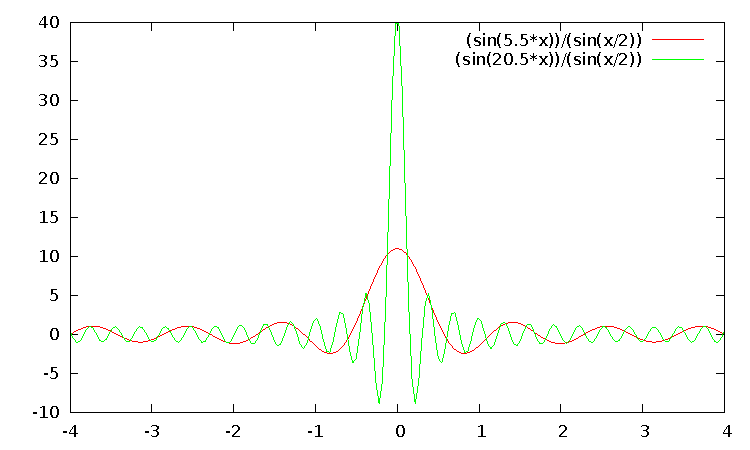
\includegraphics{dirich.pdf}
\end{center}

Note that the central peak will get taller and taller with $N$ being larger,
and the side peaks will stay small (but oscillate wildly).
Again, we are looking at in some sense an approximate delta function,
although it has
all these oscillations away from zero which do not go away.  So we expect that
$s_N$ goes to $f$.  Things are not so simple, but under some conditions on
$f$, such a conclusion holds.

People write
$$
\delta(x) \sim \sum_{n=\infty}^\infty e^{inx}
$$
although we can't say that as
we have not really defined the delta function, no a Fourier series of
whatever kind object it is.


\medskip

\textbf{Theorem 8.14:}
Let $x$ be fixed and let $f$ be Riemann integrable on $[-\pi,\pi]$.  Suppose that there exist $\delta > 0$ and $M$ such that
$$
\abs{f(x+t)-f(x)} \leq M \abs{t}
$$
for all $t \in (-\delta,\delta)$, then
$$
\lim_{N \to \infty} s_N(f;x) = f(x) .
$$

\medskip

In other words, if for example $f$ is differentiable at $x$
then we obtain convergence.  Generally what the result implies is
that if the function is continuous
piecewise smooth, then the Fourier series converges
(pointwise).   By continuous piecewise smooth we mean that $f$
is continuous and periodic so $f(-\pi) = f(\pi)$ and furthermore
that there are points $x_0 = -\pi < x_1 < \cdots < x_k = \pi$
such that $f$ restricted to $[x_j,x_{j+1}]$
is continuously differentiable (up to the endpoints) for all $j$.

\medskip

\begin{proof}
We notice that for all $N$ we get
\begin{equation*}
\frac{1}{2\pi} \int_{-\pi}^\pi D_N = 1 .
\end{equation*}
Write
\begin{equation*}
\begin{split}
s_N(f;x)-f(x) & =
\frac{1}{2\pi} \int_{-\pi}^\pi f(x-t) D_N(t) \, dt 
-
f(x)
\frac{1}{2\pi} \int_{-\pi}^\pi D_N(t) \, dt
\\
& = 
\frac{1}{2\pi} \int_{-\pi}^\pi \bigl( f(x-t) - f(x) \bigr) D_N(t) \, dt 
\\
& = 
\frac{1}{2\pi} \int_{-\pi}^\pi \frac{f(x-t) - f(x)}{\sin(t/2)} \sin\bigl(
(N+\nicefrac{1}{2})t \bigr) \, dt 
\end{split}
\end{equation*}
Now by the hypotheses we obtain that
for small nonzero $t$ we get
\begin{equation*}
\abs{ \frac{f(x-t) - f(x)}{\sin(t/2)} }
\leq
\frac{M\abs{t}}{\abs{\sin(t/2)}}
\end{equation*}
As $\sin(t) = t + h(t)$ where $\frac{h(t)}{t} \to 0$ as $t \to 0$,
we notice that
$\frac{M\abs{t}}{\abs{\sin(t/2)}}$ is continuous at the origin
and hence 
$\frac{f(x-t) - f(x)}{\sin(t/2)}$ must be bounded near the origin.
As $t=0$ is the only place on $[-\pi,\pi]$ where the denominator vanishes,
it is the only place where there could be a problem.  The function is
also Riemann integrable.  Now we use a trigonometric identity
that follows from the definition (and you've seen it on the homework
actually) that 
$$
\sin\bigl( (N+\nicefrac{1}{2})t \bigr)
=
\cos(t/2) \sin(Nt) + 
\sin(t/2) \cos(Nt)
$$
so
\begin{equation*}
\begin{split}
\frac{1}{2\pi} \int_{-\pi}^\pi \frac{f(x-t) - f(x)}{\sin(t/2)} \sin\bigl(
(N+\nicefrac{1}{2})t \bigr) \, dt 
=
&
\frac{1}{2\pi} \int_{-\pi}^\pi
\left( \frac{f(x-t) - f(x)}{\sin(t/2)}
\cos (t/2) \right) \sin (Nt) \, dt
\\
& +
\frac{1}{2\pi} \int_{-\pi}^\pi \bigl( f(x-t) - f(x) \bigr)
\cos (Nt) \, dt
\end{split}
\end{equation*}
Now 
$\frac{f(x-t) - f(x)}{\sin(t/2)} \cos (t/2)$
and
$\bigl( f(x-t) - f(x) \bigr)$ are bounded Riemann integrable functions
and so their Fourier coefficients go to zero by Theorem 8.12.  So the two
integrals on the right hand side, which compute the Fourier coefficients
for the real version of the Fourier series go to 0 as $N$ goes to infinity.
This is because $\sin(Nt)$ and $\cos(Nt)$ are also orthonormal systems.
with respect to the same inner product.
Hence $s_N(f;x)-f(x)$ goes to 0 and so $s_N(f;x)$ goes to $f(x)$.
\end{proof}

\medskip

In particular this has the following corollary:

\medskip

\textbf{Corollary:}
If $f(x) = 0$ on an entire open interval $J$, then $\lim s_N(f;x) = 0$
for all $x \in J$.

\medskip

In other words, if two functions $f$ and $g$
are equal on an open interval $J$, then the
points on $J$ where $\{ s_N(f;x) \}$ and $\{ s_N(g;x) \}$ converge are the same.  That is,
convergence at $x$ is only dependent on the values of the function
near $x$.

\medskip

We have seen Theorem 8.15 as an example for Stone-Weierstrass theorem.
That is, any continuous function on $[-\pi,\pi]$ can be uniformly approximated
by trigonometric polynomials.  However, these trigonometric polynomials need
not be the partial sums $s_N$.  On the other hand, (exercise 15) they can be
explicitly constructed from $s_N$.

\medskip

We have that the convergence always happens in the $L^2$ sense and
furthermore that formal operations on the (infinite) vectors of
Fourier coefficients is the same as the operations using the integral
inner product.

\medskip

We will mostly sketch out the proof and leave some details to the reader
as exercises.  Some of these are exercises in Rudin.

%FIXME: Should we prove $L^2$ triang and CS?  This is just formal nonsense

\medskip

\textbf{Theorem 8.16:} (Parseval)
Let $f$ and $g$ be Riemann integrable $2\pi$-periodic functions
with
$$
f(x) \sim
\sum_{n=-\infty}^\infty c_n e^{inx}
\qquad \text{and} \qquad
g(x) \sim
\sum_{n=-\infty}^\infty d_n e^{inx} .
$$
Then
$$
\lim_{N\to\infty} \snorm{f-s_N(f)}_2^2 = 
\lim_{N\to\infty}
\frac{1}{2\pi}
\int_{-\pi}^\pi
\abs{f(x)-s_N(f;x)}^2 \, dx
=0 .
$$
Also
$$
\langle f , g \rangle =
\frac{1}{2\pi}
\int_{-\pi}^\pi
f(x) \overline{g(x)}\, dx
=
\sum_{n=-\infty}^\infty c_n \overline{d_n} ,
$$
and
$$
\snorm{f}_2^2
=
\frac{1}{2\pi}
\int_{-\pi}^\pi
\abs{f(x)}^2 \, dx
=
\sum_{n=-\infty}^\infty \abs{c_n}^2.
$$

\medskip

We will skip the proof in lecture.

\begin{proof}
It is not hard too prove (Exercise 12 in chapter 6) that there is
a continuous $2\pi$-periodic function $h$ such that
$$
\snorm{f-h}_2 < \epsilon .
$$
Now we know that we can approximate $h$ with a trigonometric polynomial
uniformly, that is there is a trigonometric polynomial $P(x)$
such that
$\abs{h(x) - P(x)} < \epsilon$ for all $x$.
Hence
$$
\snorm{h-P}_2 \leq \epsilon.
$$
If $P$ is of degree $N_0$ then for all $N \geq N_0$ we have
$$
\snorm{h-s_N(h)}_2 \leq \snorm{h-P}_2 \leq \epsilon
$$
as $s_N(h)$ is the best approximation for $h$ in $L^2$ (Theorem 8.11).
Next by the inequality leading up to Bessel we have
$$
\snorm{s_N(h)-s_N(f)}_2
=
\snorm{s_N(h-f)}_2
\leq
\snorm{h-f}_2 \leq \epsilon
$$
It is not difficult (exercise 11 in chapter 6) to show the triangle
inequality for the $L^2$ norm, that is
$$
\snorm{f-s_N(f)}_2
\leq
\snorm{f-h}_2
+
\snorm{h-s_N(h)}_2
+
\snorm{s_N(h)-s_N(f)}_2
\leq 3\epsilon .
$$
For all $N \geq N_0$.

Next
$$
\langle s_N(f) , g \rangle
=
\frac{1}{2\pi}
\int_{-\pi}^\pi
s_N(f;x) \overline{g(x)} \, dx
=
\sum_{k=-N}^N
c_k 
\frac{1}{2\pi}
\int_{-\pi}^\pi
e^{ikx}
\overline{g(x)} \, dx
=
\sum_{k=-N}^N
c_k 
\overline{d_k}
$$
Next we need the Schwarz (or Cauchy-Schwarz)
inequality (left as exercise), that is
$$
{\abs{\int_a^b f\bar{g}}}^2
\leq
\left( \int_a^b \abs{f}^2 \right)
\left( \int_a^b \abs{g}^2 \right)
$$
This is left as an exercise.  It actually follows by purely formal
linear algebra using simple the idea that the integral gives an inner
product.
So
%Next let $M$ be such that $\abs{g(x)} \leq M$ for all $x$,
%($g$ is Riemann integrable so bounded)
$$
\abs{\int_{-\pi}^\pi f\bar{g} - \int_{-\pi}^\pi s_N(f)g}
=
\abs{\int_{-\pi}^\pi (f- s_N(f))g}
\leq
\int_{-\pi}^\pi \abs{f- s_N(f)}\, \abs{g}
\leq
{\left(\int_{-\pi}^\pi \abs{f- s_N(f)}^2 \right)}^{1/2}
{\left( \int_{-\pi}^\pi \abs{g}^2 \right)}^{1/2} .
$$
Now the right hand side goes to 0 as $N$ goes to infinity.
\end{proof}


%%%%%%%%%%%%%%%%%%%%%%%%%%%%%%%%%%%%%%%%%%%%%%%%%%%%%%%%%%%%%%%%%%%%%%%%%%%%%%
%%%%%%%%%%%%%%%%%%%%%%%%%%%%%%%%%%%%%%%%%%%%%%%%%%%%%%%%%%%%%%%%%%%%%%%%%%%%%%
%%%%%%%%%%%%%%%%%%%%%%%%%%%%%%%%%%%%%%%%%%%%%%%%%%%%%%%%%%%%%%%%%%%%%%%%%%%%%%

\chapter{Lebesgue integral} \label{lebesgue:chapter}

%\vspace*{-3in}
%{\large DRAFT~~~~DRAFT~~~~DRAFT~~~~DRAFT~~~~\today}
%\vspace*{2.508in}

%%%%%%%%%%%%%%%%%%%%%%%%%%%%%%%%%%%%%%%%%%%%%%%%%%%%%%%%%%%%%%%%%%%%%%%%%%%%%%

\section{FIXME}
\label{sec:FIXME}

\sectionnotes{FIXME lectures}

We will define a very powerful integral, far better than Riemann in the
sense that it will allow us to integrate pretty much every reasonable
function and we will also obtain strong convergence results.  That is
if we take a limit of integrable functions we will get an integrable
function and the limit of the integrals will be the integral of the limit
under very mild conditions.  We will focus only on the real line, although
the theory easily extends to more abstract contexts.

\medskip

In Riemann integral the basic block was a rectangle.  If we wanted to
integrate a function that was identically 1 on an interval $[a,b]$, then the
integral was simply the area of that rectangle, so $1 \times (b-a) = b-a$.
For Lebesgue integral what we want to do is to replace the interval with a
more general subset of the real line.  That is, if we have a set $S \subset
\R$ and we take the \emph{indicator function} or \emph{characteristic
function} $\chi_S$ defined by
$$
\chi_S (x) =
\begin{cases}
1 & \text{ if $x \in S$,} \\
0 & \text{ else.}
\end{cases}
$$
Then the integral of $\chi_S$ should really be equal to the area under the
graph, which should be equal to the ``size'' of $S$.

\medskip

\textbf{Example:}
Suppose that $S$ is the set of rational numbers between $0$ and $1$.  Let us
argue that its size is 0, and so the integral of $\chi_S$ should be 0.
Let $\{ x_1, x_2, \ldots \} = S$ be an enumeration
of the points of $S$.  Now for any $\epsilon > 0$
take the sets
$$I_j = (x_j - \epsilon 2^{-j-1}, 
x_j + \epsilon 2^{-j-1}),$$
then
$$
S \subset \bigcup_{j=1}^\infty I_j .
$$
The ``size'' of any $I_j$ should be $\epsilon 2^{-j}$, so it seems reasonable
to say that the ``size'' of $S$ is less than the sum of the sizes of the $I_j$'s.
At worst we are grossly overestimating; every $I_j$ contains
infinitely
many other points of $S$, so there is a lot of overlap.  So
$$
\text{``size of $S$''} \leq
\sum_{j=1}^\infty \text{ ``size of $I_j$''} =
\sum_{j=1}^\infty \epsilon 2^{-j} = \epsilon.
$$
So the ``size of $S$'' (whatever that concept should be) seems like it ought
to be 0.  And hence the integral of $\chi_S$ should be 0.

\medskip

So to begin, we want to have a way to ``measure'' sets.  We focus
only on the real numbers and so suppose we wish to measure subsets of the real
numbers.  We would like (our Christmas wish) to have a function
$$
m \colon \sP(\R) \to [0,\infty]
$$
that is a function that takes subsets of the real numbers
and gives nonnegative extended real numbers, such that 
$$
m(\emptyset) = 0
$$
and if $\{ S_j \}$ is a countable collection of pairwise disjoint sets then
$$
\sum_{j=1}^\infty m(S_j) = m\left( \bigcup_{j=1}^\infty S_j \right)
$$
It should also replicate what we normally think of size of intervals,
that is $m( (a,b) ) = m([a,b) ) = m([a,b]) = m((a,b]) = b-a$.

Unfortunately, such a function is impossible.  At least there is
no such function on all of $\sP(\R)$ (the power set of the reals).
We do have such a function on a subset of the powerset.  That is,
we will define a smaller set of subsets called measurable sets
and on these sets we will be able to define such a function.

So let's talk about certain collections of sets.  The collections we will
want are so called $\sigma$-algebras (Rudin talks about $\sigma$-rings, the
idea is very similar, I'll note what the difference is).

\medskip

\textbf{Definition:}
Let $X$ be a set.
A collection of sets $\sM \subset \sP(X)$ is a \emph{$\sigma$-algebra} if
\begin{enumerate}[(i)]
\item $\sM$ is nonempty,
\item $\sM$ is closed under complements, that is, if $A \in \sM$ then
$A^c = X \setminus A \in \sM$,
\item $\sM$ is closed under countable unions, that is if $\{ A_j \}$ is
a countable collection of sets in $\sM$ then
$$
\bigcup_{j=1}^\infty A_j \in \sM .
$$
\end{enumerate}
If $\sM$ is closed only under finite unions, then we say that $\sM$ is an
\emph{algebra}.

\medskip

Most of the time below we will assume that $X=\R$, so you might as well
think of subsets of the real line.

\medskip

Definition of $\sigma$-ring and ring is similar but only needs closure under
relative complements.  A $\sigma$-algebra is always a $\sigma$-ring, and a
$\sigma$-ring is a $\sigma$-algebra if it contains the whole
set $X$ as an element.

The sets in $\sM$ are usually called \emph{measurable sets}.  We will define a
certain function on the powerset and define a certain
$\sigma$-algebra on which it has the desired properties.  Our
$\sigma$-algebra will be so large that we will essentially be able to
integrate anything we want.  It will be very hard to come up with sets that
are not in our $\sigma$-algebra.

\medskip

%FIXME: used $\R^*$ in basic anal
We will work with the \emph{extended real numbers}
$\overline{\R} = \R \cup \{ -\infty, \infty \}$.  We have previously used
really only its order properties such as $-\infty < x < \infty$ for
all $x \in \R$.  Now we will also often use arithmetic on 
$\overline{\R}$.  We have to be careful as
$\overline{\R}$ will not be a field like $\R$.  In fact, some operations are
not even defined.  Let us define
\begin{align*}
& x \cdot \infty = \infty \qquad \text{for all $x > 0$} \\
& x \cdot \infty = -\infty \qquad \text{for all $x < 0$} \\
& x + \infty = \infty \quad \text{and} \quad x - \infty = -\infty \qquad
\text{for all $x \in \R$} \\
&
\frac{x}{\pm\infty} = 0
\qquad \text{for all $x \in \R$}
\end{align*}
and so on.  Everything that is not an indefinite form
$\infty - \infty$, $\frac{\pm \infty}{\pm \infty}$, or $0 \cdot \infty$
has an obvious definition.  It will be convenient for measure theory to define
$$
0 \cdot \infty = 0 .
$$
We will have to avoid $\infty - \infty$ and
$\frac{\pm \infty}{\pm \infty}$.

\medskip

\textbf{Definition:}
Let $\sM$ be a $\sigma$-algebra.  Let
$$
\mu \colon \sM \to \overline{\R} .
$$
We say $\mu$ is \emph{additive} if given $A, B \in \sM$,
disjoint ($A \cap B = \emptyset$) then
$$
\mu ( A \cup B) = \mu (A) + \mu(B) .
$$
We say $\mu$ is \emph{countably additive} if given $\{ A_j \}$ a collection
of sets in $\sM$ such that $A_j \cap A_k = \emptyset$ for all $j\not=k$, then
$$
\mu \left( \bigcup_{j=1}^\infty A_j \right) =
\sum_{j=1}^\infty \mu (A_j) .
$$
Of course the sums have to make sense, so usually we will assume that $\mu$
does not achieve both $-\infty$ and $\infty$.

We will say that $\mu$ is nonnegative or monotonic if $\mu(A) \geq 0$ for all $A \in \sM$.

We also say that
$\mu$ is \emph{countably subadditive} if for every collection
$\{ A_j \}$ we have
$$
\mu \left( \bigcup_{j=1}^\infty A_j \right) \leq
\sum_{j=1}^\infty \mu (A_j) .
$$

\medskip

It is not too hard to show that if $\mu$ is additive then $\mu(\emptyset) =
0$.  We also have additivity for arbitrary finite unions by induction.

If $B \subset A$ and $\mu(B)$ is finite, then
writing $A = B \cup (A\setminus B)$ we obtain that 
$$
\mu(A\setminus B) = \mu(A) - \mu(B) .
$$

Another useful property for additive functions is
$$
\mu(A \cup B) + \mu(A \cap B) = \mu(A) + \mu(B) .
$$
This follows by looking at the disjoint unions
$B = (B \setminus A) \cup (A \cap B)$ and noting that $A \cup B = A \cup (B
\setminus A)$.  So for example a nonnegative additive function is
also (finitely) subadditive:
$$
\mu(A \cup B) \leq \mu(A) + \mu(B) .
$$

Countably additive functions are additive of course.
Also, countably additive $\mu$ play nicely with limits.

\medskip

\textbf{Theorem 11.3:}
Suppose that $\mu$ is a countably additive function on a $\sigma$-algebra
$\sM$ and $A_1 \subset A_2 \subset \cdots$ are sets in $\sM$
and $A = \cup_j A_j$, then
$$
\lim_{n \to \infty} \mu(A_n) = \mu (A) ,
$$
where the limit has the obvious interpretation for $\infty$ (or $-\infty$).

\medskip

\begin{proof}
Write $B_1 = A_1$ and $B_j = A_j \setminus A_{j-1}$.
Then the $B_j$'s are pairwise disjoint and $A = \cup_j B_j$, so
$$
\mu(A) = \sum_{j=1}^\infty \mu(B_j) .
$$
As $A_n = B_1 \cup B_2 \cup \cdots \cup B_n$ then
$$
\mu(A_n) = \sum_{j=1}^n \mu(B_j) ,
$$
and the result follows.
\end{proof}

\medskip

\textbf{Definition:}
If we have a $\sigma$-algebra $\sM$ of measurable sets, then we call a
function
$$
\mu \colon \sM \to \overline{\R}
$$
a \emph{measure} if it is a nonnegative and countably additive.  Sometimes
$\mu(\emptyset) = 0$ is also given as requirement, but that follows from
additivity.  Also some authors require $\mu$ to not be identically zero.

\medskip

It turns out there are many different measures.  The simplest measure can be
defined as follows.  Let $\sM$ be all of $\sP(X)$, and define
$\mu(A) = \abs{A}$, the cardinality of $A$.  This $\mu$ is called the
\emph{counting measure}.  Despite how trivial this example
is, it does happen to be useful; we will see it later on.

\medskip

Let us construct the Lebesgue measure.  What we will actually construct
is a subadditive nonnegative function on all of $\sP(\R)$, which will turn out to be a
measure (so countably additive) on some large $\sigma$-algebra in $\sP(\R)$.

\medskip

Let us define a bounded interval to be a set of the form
$$
\{ x : a < x < b \}
\qquad \text{or} \qquad
\{ x : a \leq x < b \}
\qquad \text{or} \qquad
\{ x : a < x \leq b \}
\qquad \text{or} \qquad
\{ x : a \leq x \leq b \}
$$
for real numbers $a \leq b$.  We allow $a = b$, meaning we allow 
$\emptyset$ and the single point set $\{ x \}$ to also be intervals.
If $I$ is a bounded interval, define
$$
m(I) = b-a .
$$

%Let $\sE$ be the set of finite unions of pairwise disjoint intervals.  If $A = 
%I_1 \cup I_2 \cup \cdots \cup I_n$ is a pairwise disjoint union of intervals
%then define
%$$
%m(A) = m(I_1)+\cdots +m(I_n) .
%$$
%It is not hard to see that $m$ is well defined and
%that $m$ is a nonnegative additive function on the algebra $\sE$
%(not a $\sigma$-algebra).  Also $m$ is finite on $\sE$.
%Sets in $\sE$ are called elementary sets.
%
%\medskip
%
%We claim the function $m$ is a so-called \emph{regular} function on $\sE$.  That is,
%for any $A \in \sE$, and every $\epsilon > 0$ there are
%a closed set $F$ and an open set $G$ in $\sE$, with $F \subset A \subset G$
%such that
%$$
%m(G) - \epsilon \leq m(A) \leq m(F) + \epsilon .
%$$
%The claim follows by noting that the property is not hard to show for an
%interval.

It is easy to see that given any bounded interval $I$
and any $\epsilon > 0$, there are
a closed interval $F$ and an open interval $G$, with $F \subset A \subset G$
such that
$$
m(G) - \epsilon \leq m(I) \leq m(F) + \epsilon .
$$

Now the point is to show that we can extend $m$ to a countably additive
function on a $\sigma$-algebra that contains all the intervals.%$\sE$.

Let $E \subset \R$ be any set.  Let $\{ I_j \}$ be a countable
collection of bounded open intervals covering $E$,
that is
$$
E \subset \bigcup_{j=1}^\infty I_j .
$$
Define the \emph{outer measure}
as
$$
m^*(E) = \inf \sum_{j=1}^\infty m(I_j) ,
$$
where the $\inf$ is taken over all coverings of $E$ by countably many bounded open
intervals.

It is immediate that $m^*$ is nonnegative ($m^*(A) \geq 0$) and monotone (if $A \subset B$
then $m^*(A) \leq m^*(B)$).

\medskip

\textbf{Theorem 11.8:}
If $I$ is a bounded interval, then $m(I) = m^*(I)$.  Also $m^*$ is countably subadditive.

\medskip

That is $m^*$ is a countably subadditive extension of $m$.

\medskip

\begin{proof}
Suppose that $I$ is a bounded interval, and let $\epsilon > 0$ be given.
Then there exists an open bounded interval $G$, $I \subset G$, such that
$m(G) \leq m(I) + \epsilon$.
As $G$ is a covering of $I$ by bounded open intervals,
$$
m^*(I) \leq m(G) .
$$
So $m^*(I) \leq m(G) \leq m(I) + \epsilon$.  As $\epsilon > 0$
was arbitrary we have $m^*(I) \leq m(I)$.
By definition of $m^*$ there exists a sequence
of open bounded intervals $\{ G_j \}$ covering $I$ such that
$$
\sum_{j=1}^\infty m(G_j) \leq m^*(I) + \epsilon .
$$
There also exists a bounded closed interval $F$, $F \subset I$, such that
$m(F) \geq m(I)-\epsilon$.
As $F$ is compact, there is some $N$ such that
$$
F \subset G_1 \cup G_2 \cup \cdots \cup G_N .
$$
and so
$$
m(I) \leq \epsilon+m(F) \leq \epsilon + \sum_{j=1}^N m(G_j)
\leq 
\epsilon + \sum_{j=1}^\infty m(G_j) \leq m^*(I) + 2\epsilon .
$$
So $m(I) \leq m^*(I)$.  Thus $m(I) = m^*(I)$.

\medskip

Let us show countable subadditivity.
Suppose that $A = \cup_{j=1}^\infty A_j$.
If $m^*(A_j) = \infty$ for any $j$, then we are done, so suppose that
$m^*(A_j)$ is finite for every $j$.

Each $A_j$
has a covering $G_{jk}$ of bounded open intervals such that
$$
\sum_{k=1}^\infty m(G_{jk}) \leq m^*(A_j) + \epsilon 2^{-j} .
$$
So as all the $G_{jk}$ together cover $A$
$$
m^*(A)
\leq
\sum_{j=1}^\infty
\sum_{k=1}^\infty
m(G_{jk})
\leq
\sum_{j=1}^\infty
\Bigl( m^*(A_j) + \epsilon 2^{-j} \Bigr)
\leq
\left(
\sum_{j=1}^\infty
m^*(A_j) \right)
+ \epsilon .
$$
\end{proof}

Note that by the same argument as for the example we started the section
with, we have:

\medskip

\textbf{Corollary:}
If $S \subset \R$ is countable, then $m^*(S) = 0$.

\medskip

It will be useful to have the following result about open subsets of $\R$:

\medskip

\textbf{Proposition:}
An open subset $W \subset \R$ is a countable union of pairwise
disjoint open intervals.

\medskip

\begin{proof}
For each point $x \in W$, let $I_x$ be the largest open interval such
that $I_x \subset W$ and $x \in I_x$ (that is, $I_x$ is the union of all
open intervals contained in $W$ that contain $x$).  Every $I_x$ contains
rational points.  Furthermore if $y \in I_x$, then $I_y = I_x$.  So
$$
W = \bigcup_{x \in \Q \cap W} I_x
$$
We take some enumeration of the rationals and pick one rational
point in every $I_x$, then we have $W$ written as a countable union of
pairwise disjoint open intervals.
\end{proof}

\medskip

Here we depart a little from Rudin again to have a simpler definition:

\textbf{Definition:}
A set $E \subset \R$ is said to be \emph{Lebesgue measurable}
if for each subset $A \subset \R$ we get
$$
m^*(A) = m^*(A \cap E) + m^*(A \cap E^c) .
$$
We will denote the measurable sets by $\sM$.  And unless otherwise stated
(that is, when talking about Lebesgue measure $m$ or the associated outer
measure $m^*$) $\sM$ will mean Lebesgue measurable sets.

Note that
$$
m^*(A) \leq m^*(A \cap E) + m^*(A \cap E^c)
$$
is always true by subadditivity of $m^*$.  So to show that $E$ is measurable,
what we need to show is that
$$
m^*(A) \geq m^*(A \cap E) + m^*(A \cap E^c).
$$
Furthermore, this inequality is always true when $m^*(A) = \infty$, so
we only really need to worry about $A$ such that $m^*(A) < \infty$.

If $E$ is measurable then $E^c$ is measurable by symmetry of the
condition.  It is not hard
to see that $\emptyset$ and $\R$ are measurable.

\medskip

\textbf{Proposition:}
If $m^*(E) = 0$, then $E$ is Lebesgue measurable.

\medskip

\begin{proof}
For any set $E$ we have
$$
m^*(A \cap E) \leq m^*(E)
$$
so $m^*(A \cap E) = 0$.  Also
$$
m^*(A \cap E^c) \leq m^*(A) .
$$
So
$$
m^*(A \cap E) + m^*(A \cap E^c) \leq m^*(A) .
$$
\end{proof}

\medskip

So for example countable sets and their complements are Lebesgue measurable.

\medskip

Sets of measure 0 are called \emph{null sets}.  We have seen above that all
countable subsets of $\R$ are null sets, but there exist 
uncountable null sets as well.

\medskip

\textbf{Proposition:}
The set of Lebesgue measurable sets
$\sM$ is an algebra of sets.

\medskip

\begin{proof}
As we said above, $\sM$ is closed under complements.  So we need to show that
it is closed under finite unions.

Let $E$ and $F$ be measurable.
Given any $A$ we have
$$
m^*(A \cap E^c) =
m^*(A \cap E^c \cap F) +
m^*(A \cap E^c \cap F^c)
=
m^*(A \cap E^c \cap F) +
m^*\bigl(A \cap ( E \cup F)^c \bigr)
$$
%and
%$$
%m^*(A \cap F^c) =
%m^*(A \cap F^c \cap E) +
%m^*(A \cap F^c \cap E^c)
%=
%m^*(A \cap E \cap F^c ) +
%m^*(A \cap ( E \cup F)^c ).
%$$
and
$$
m^*(A \cap E^c)
=
m^*(A) -
m^*(A \cap E) .
$$
Also
$A \cap (E \cup F) = (A \cap E) \cup (A \cap E^c \cap F)$ so
$$
m^*\bigl(A \cap (E \cup F) \bigr)
\leq
m^*(A \cap E ) +
m^*(A \cap E^c \cap F ) .
$$
Hence,
\begin{equation*}
\begin{split}
m^*\bigl(A \cap (E \cup F) \bigr) +
m^*\bigl(A \cap (E \cup F)^c \bigr)
& =
m^*\bigl(A \cap (E \cup F) \bigr) +
m^*(A \cap E^c ) -
m^*(A \cap E^c \cap F )
\\
& =
m^*(A)
+
m^*\bigl(A \cap (E \cup F) \bigr)
-
m^*(A \cap E ) -
m^*(A \cap E^c \cap F )
\\
& \leq
m^*(A) .
\end{split}
\end{equation*}
\end{proof}

\medskip

\textbf{Proposition:}
Let $E_1, \ldots, E_n$ be pairwise disjoint and measurable, then
for any set $A$ we have
$$
m^*\left( A \cap \left( \bigcup_{j=1}^n E_j \right) \right)
=
\sum_{j=1}^n
m^*( A \cap  E_j ) .
$$

\medskip

\begin{proof}
The set $E_n$ is measurable and hence
\begin{equation*}
\begin{split}
m^*\left( A \cap \left( \bigcup_{j=1}^n E_j \right) \right)
& =
m^*\left( A \cap \left( \bigcup_{j=1}^n E_j \right) \cap E_n \right)
+
m^*\left( A \cap \left( \bigcup_{j=1}^n E_j \right) \cap E_n^c \right)
\\
& =
m^*( A \cap E_n )
+
m^*\left( A \cap \left( \bigcup_{j=1}^{n-1} E_j \right) \right)
\end{split}
\end{equation*}
and the proof follows by induction.
\end{proof}

\medskip

\textbf{Theorem:}
The set of Lebesgue measurable sets is a $\sigma$-algebra.

\medskip

\begin{proof}
Suppose that $E = \cup_{j=1}^\infty E_j$ where all the $E_j$
are measurable.  Define $F_1 = E_1$ and
$F_j = E_j \setminus \cup_{k=1}^{j-1} E_{k}$.  We have that $F_j$
is measurable for every $j$ as $\sM$ is an algebra.  We have that $F_j \cap F_k = \emptyset$
if $j \not= k$, and also that $E = \cup_{j=1}^\infty F_j$.

Let $A$ be any set.  Then,
\begin{equation*}
\begin{split}
m^*(A)
& =
m^*\left(A \cap \bigcup_{j=1}^n F_j\right)
+
m^*\left(A \cap {\left(\bigcup_{j=1}^n F_j\right)}^c\,\right)
\\
& \geq
m^*\left(A \cap \bigcup_{j=1}^n F_j\right)
+
m^*(A \cap E^c)
\\
& =
\sum_{j=1}^n
m^*(A \cap F_j)
+
m^*(A \cap E^c) .
\end{split}
\end{equation*}
Taking limits we have
\begin{equation*}
\begin{split}
m^*(A)
\geq
\sum_{j=1}^\infty
m^*(A \cap F_j)
+
m^*(A \cap E^c)
\geq
m^*\left(A \cap \bigcup_{j=1}^\infty F_j\right)
+
m^*(A \cap E^c)
=
m^*(A \cap E)
+
m^*(A \cap E^c) .
\end{split}
\end{equation*}
So $E$ is measurable.
\end{proof}

\medskip

\textbf{Theorem:}
All intervals are Lebesgue measurable, and hence all open sets are
measurable.

\medskip

\begin{proof}
Let $I$ be an interval of the form
$(-\infty,x)$, $(-\infty,x]$,
$(x,\infty)$, or $[x,\infty)$.
Let $\epsilon > 0$ be given and
$A$ be an arbitrary set such that
$m^*(A) < \infty$.  Let $\{ I_n \}$
be a countable collection of open bounded intervals such that
$$
A \subset \bigcup_{j=1}^\infty I_j ,
$$
and such that
$$
\sum_{j=1}^\infty m(I_j) \leq m^*(A) + \epsilon .
$$
Note that $I_j \cap I$ and
$I_j \cap I^c$ are bounded intervals (could be empty).
We have
\begin{align*}
m^*(A \cap I)
& \leq
\sum_{j=1}^\infty m(I_j \cap I) , \qquad \text{and}
\\
m^*(A \cap I^c)
& \leq
\sum_{j=1}^\infty m(I_j \cap I^c) .
\end{align*}
We have that $m(I_j) = m(I_j \cap I) + m(I_j \cap I^c)$.
So
$$
m^*(A \cap I)
+
m^*(A \cap I^c)
\leq
\sum_{j=1}^\infty m(I_j)
\leq m^*(A) + \epsilon .
$$
As $\epsilon > 0$ was arbitrary we obtain the required inequality.
If $m^*(A) = \infty$ the inequality was trivial.

Any bounded interval is an intersection of two half infinite intervals as
above, and so is measurable.
Any open set is a countable union of open intervals, and so it is also
measurable.
\end{proof}

\medskip

We of course also get that all closed sets are measurable.  But we get a lot
more.  We get that countable unions of closed sets are measurable, and so are
countable intersections of open sets, and so on and so forth.

It is not hard to prove that an intersection of $\sigma$-algebras is
still a $\sigma$-algebra.  Therefore, there exists a smallest
$\sigma$-algebra that contains the open sets (it's the intersection of all
$\sigma$-algebras containing the open sets).  This $\sigma$-algebra
is denoted by $\sB$ and the sets in it are called
the \emph{Borel sets}.  As $\sB \subset \sM$, we have that all Borel sets
are measurable.  Sometimes it is just convenient to talk about
$\sB$ rather than $\sM$.

\medskip

Let us now define 
$$
m \colon \sM \to [0,\infty]
$$
by defining $m(E) = m^*(E)$.  As $m^*$ agreed with the earlier definition of
$m$ on intervals,
this new $m$ agrees with our earlier definition of $m$ (on intervals).
We have still not shown that $m$ is a measure on $\sM$.
We call $m$ the \emph{Lebesgue measure} (we will show momentarily that it
really is a measure, so the name is justified).

\medskip

\textbf{Theorem (like 11.10 in Rudin):}
$m$ is countably additive, and hence a measure.

\medskip

\begin{proof}
Let $\{E_j\}$ be a family of pairwise disjoint Lebesgue measurable sets
and let $E = \cup_{j=1}^\infty E_j$.
If $m(E_j) = \infty$ for any $j$, then $m(E) = \infty$ and additivity
is trivial.  So assume that
$m(E_j) < \infty$ for all $j$.

Using $A=\R$ with an above proposition we have for any $n$
$$
m( E)
=
m\left( \bigcup_{j=1}^\infty E_j  \right)
\geq
m\left( \bigcup_{j=1}^n E_j  \right)
=
\sum_{j=1}^n
m( E_j ) .
$$
Taking limits we have
$$
m( E)
\geq
\sum_{j=1}^\infty
m( E_j ) .
$$
The opposite inequality follows by subadditivity.
\end{proof}

\medskip

\textbf{Proposition:}
If $E \subset \R$ is Lebesgue measurable, then for every $\epsilon > 0$
there exist an open set $G$ and a closed set $F$
such that $F \subset E \subset G$,
$$
m(E \setminus F) < \epsilon , \qquad \text{and} \qquad
m(G \setminus E) < \epsilon .
$$

\medskip

\begin{proof}
If $m(E) < \infty$ then $G$ is found directly by definition of $m^*$.
If $m(E) = \infty$, then we have to work a little harder.  So look at the
sets $E_j = E \cap [j,j+1)$.  We have that $m(E_j) \leq m\bigl([j,j+1)\bigr)
< 1 < \infty$, and $E = \cup_{j=-\infty}^\infty E_j$.  For every $j$ we can find an open set
$G_j$ such that, $E_j \subset G_j$ and $m(G_j \setminus E_j) < \epsilon
2^{-\abs{j}}$.
Let $G = \cup_{j=-\infty}^\infty G_j$.
So
$$
m(G \setminus E)
=
m\left( \bigcup_{j=-\infty}^\infty ( G_j\setminus E) \right)
\leq
m\left( \bigcup_{j=-\infty}^\infty ( G_j\setminus E_j) \right)
\leq
\sum_{j=-\infty}^\infty
m( G_j\setminus E_j)
<
\sum_{j=-\infty}^\infty
\epsilon 2^{-\abs{j}}
=
3\epsilon .
$$

Then to
find $F$, take the complement $E^c$ and find an open set that covers it
and take a complement of that.  Details are left to student.
\end{proof}

\medskip

We remark that by letting $\epsilon$ go to 0, we can show (left to
students) that there exists a Borel set $G$ that is a countable intersection
of open sets, and a Borel set $F$ that is a countable union of closed sets,
such that $F \subset E \subset G$
$$
m(E \setminus F) = m(G \setminus E) = 0 .
$$
Note that, of course, $m(E)=m(F)=m(G)$.
So every Lebesgue measurable set is almost like a Borel set; the difference
is a null set.
 
\medskip

\textbf{Measurable functions}

\medskip

If we want to integrate functions, we want to know which functions play
nicely with the measure, or actually with the measurable sets.
For example if $S$ is a nonmeasurable set, then we don't expect
to be able to integrate the characteristic function $\chi_S$, as its integral
should be the measure of $S$.

\medskip

Let us work in a general \emph{measurable space}
$(X,\sM)$, that is, a set $X$ and a $\sigma$-algebra of sets $\sM$.
If you want to, you can think of $(\R,\sM)$, where $\sM$ are the Lebesgue
measurable sets.  Note that we will not worry about the actual measure.

\medskip

\textbf{Definition 11.13:}
Let $(X,\sM)$ is a measurable space.  $f \colon X \to \overline{\R}$ is said
to be \emph{measurable} %(or measurable with respect to $\sM$)
if
$$
f^{-1} \bigl( (a,\infty] \bigr)
=
\{ x \in X : f(x) > a \}
\in \sM
$$
for all $a \in \R$.

\medskip

If $X=\R$ and $\sM$ is the set of Lebesgue measurable sets, then
we say that $f$ is said to be \emph{Lebesgue measurable}.  If $X=\R$ and
$\sM =\sB$ is the $\sigma$-algebra of Borel sets, then
$f$ is said to be \emph{Borel measurable}.  Note that if a function is
Borel measurable then it is, of course, Lebesgue measurable.

When people speak of just ``measurable'' functions on the real line, they will
generally mean Lebesgue measurable.

\medskip

\textbf{Proposition:}
If $f \colon \R \to \R$ is continuous, then 
it is Borel measurable
(and hence Lebesgue measurable).

\medskip

\begin{proof}
The interval $(a,\infty)$ is open and so
$f^{-1}\bigl( (a,\infty) \bigr)$ is open and so Borel (and so Lebesgue
measurable as well).
\end{proof}

\medskip

\textbf{Theorem 11.15:}
Let $(X,\sM)$ is a measurable space and $f \colon X \to \overline{\R}$ 
a function.
The following are equivalent:
\begin{enumerate}[(i)]
\item $f$ is measurable, that is $\{ x \in X : f(x) > a \}$ is measurable for
all $a \in \R$.
\item $\{ x \in X : f(x) \geq a \}$ is measurable for all $a \in \R$.
\item $\{ x \in X : f(x) < a \}$ is measurable for all $a \in \R$.
\item $\{ x \in X : f(x) \leq a \}$ is measurable for all $a \in \R$.
\end{enumerate}

\medskip

\begin{proof}
The implications (i) implies (ii) implies (iii) implies (iv) implies (i)
are shown by the following equalities:
\begin{align*}
& \{ x \in X : f(x) \geq a \} = \bigcap_{n=1}^\infty
\{ x \in X : f(x) > a - \nicefrac{1}{n} \} ,
\\
&
\{ x \in X : f(x) < a \} = X \setminus \{ x \in X : f(x) \geq a \} ,
\\
&
\{ x \in X : f(x) \leq a \} = \bigcap_{n=1}^\infty
\{ x \in X : f(x) < a  + \nicefrac{1}{n} \} ,
\\
&
\{ x \in X : f(x) > a \} = X \setminus \{ x \in X : f(x) \leq a \} .
\end{align*}
\end{proof}

\medskip

Similarly we also can prove that $f^{-1} (\{\infty\})$ and
$f^{-1}(\{-\infty\})$ are measurable.  So we could let $a$ vary over all of
$\overline{\R}$.

\medskip

\textbf{Theorem 11.16 (and corollary):}
Let $(X,\sM)$ is a measurable space and $f \colon X \to \overline{\R}$
and $g \colon X \to \overline{\R}$ are measurable then
\begin{enumerate}[(i)]
\item $\abs{f}$ is measurable.
\item $\max(f,g)$ and $\min(f,g)$ are measurable.
\item $f^+ = \max(f,0)$ and $f^-=-\min(f,0)$ are measurable.  (Note that
$f = f^+ - f^-$ and $\abs{f} = f^+ + f^-$)
\end{enumerate}

\begin{proof}
First item follows by
$
\{ x : \abs{f(x)} < a \} = \{ x : f(x) < a \} \cap \{ x : f(x) > -a \}
$

Second item follows by writing
$
\{ x : \max(f,g) (x) < a \} = \{ x : f(x) < a \} \cap \{ x : g(x) < a \}
$
and
$
\{ x : \min(f,g) (x) < a \} = \{ x : f(x) < a \} \cup \{ x : g(x) < a \}
$.

Last item follows by the second item.
\end{proof}

\medskip

In fact essentially any reasonable (see below about composition) operation we do to measurable functions
lands us back in the set of measurable functions.

\medskip

\textbf{Theorem 11.17:}
Let $(X,\sM)$ is a measurable space and
let $\{ f_n \}$ be a sequence of measurable functions defined on $X$.  
Define
\begin{align*}
& g_1(x) = \sup_{n \in \N} f_n(x) , \\
& g_2(x) = \inf_{n \in \N} f_n(x) , \\
& g_3(x) = \limsup_{n \to \infty} f_n(x) , \\
& g_4(x) = \liminf_{n\to\infty} f_n(x) .
\end{align*}
Then $g_1$, $g_2$, $g_3$, and $g_4$ are all measurable.   In particular, if
$\{f_n\}$ converges pointwise to $f$, then $f$ is measurable.

\medskip

\begin{proof}
If $g_1(x) > a$, then there is some $n$ such that
$f_n(x) > a$.  Similarly, if $f_n(x) > a$ for some $n$,
then obviously $g_1(x) > a$.  So
$$
\{ x : g_1(x) > a \}
=
\{ x : \sup_{n \in \N} f_n(x) > a \}
= \bigcup_{n=1}^\infty \{ x : f_n(x) > a \} .
$$
In other words $g_1$ is measurable.

Similarly,
$$
\{ x : g_2(x) < a \}
=
\{ x : \inf_{n \in \N} f_n(x) < a \}
= \bigcup_{n=1}^\infty \{ x : f_n(x) < a \} .
$$
So $g_2$ is measurable.

Next notice that
\begin{align*}
& g_3(x) =
\limsup_{n \to \infty} f_n(x)
=
\inf_{m \in \N} \left( \sup_{n \geq m} f_n(x) \right) ,
\\
& g_4(x) =
\liminf_{n \to \infty} f_n(x)
=
\sup_{m \in \N} \left( \inf_{n \geq m} f_n(x) \right) .
\end{align*}
So $g_3$ and $g_4$ are also measurable.

If the sequence is convergent, then limit is equal to limsup (or liminf) and
hence $f$ is measurable.
\end{proof}

Composition is somewhat tricky.  Even if $f \colon \R \to \R$ and
$g \colon \R \to \R$ are Lebesgue
measurable, doesn't mean that $f \circ g$ is measurable.
First we notice that what really happens is that a Lebesgue
measurable function
is a function that takes Borel sets on $\R$ into Lebesgue measurable
sets, that is, if $A$ is a Borel set
then $g^{-1}(A)$ is Lebesgue measurable.
The inverse image of a Lebesgue measurable set need not be Lebesgue measurable
for a Lebesgue measurable function.  We would need something stronger:

\medskip

\textbf{Proposition:}
If $f \colon \R \to \R$ and
$g \colon \R \to \R$ are both Borel measurable, then $f \circ g$
is Borel measurable.

\medskip

The proof is left to student.
%You can also prove that if $f$
%is Borel measurable and $g$ is Lebesgue measurable then
%$f \circ g$ is Lebesgue measurable.
On the other hand there exist
examples of even a continuous $g$ and Lebesgue measurable $f$
so that $f \circ g$ is not Lebesgue measurable.

\medskip

\textbf{Theorem 11.18:}
Let $(X,\sM)$ is a measurable space,
$f \colon X \to \R$ and $g \colon X \to \R$ be measurable functions,
and $F \colon \R^2 \to \R$ be a continuous function, then
$h(x) = F\bigl(f(x),g(x)\bigr)$ is a measurable function.

In particular $f+g$ and $fg$ are measurable.

\medskip

\begin{proof}
Fix $a \in \R$, then look at the open set
$$
G = \{ (y_1,y_2) : F(y_1,y_2) > a \} .
$$
An open set contains a whole ball around every 
point.  So for every point $y=(y_1,y_2)$ in $G$
there is a $\delta > 0$ such that
$$
\{ (z_1,z_2) : y_1 - \delta < z_1 < y_1 +\delta, ~
y_2 - \delta < z_2 < y_2 +\delta \} \subset G .
$$
Since $\R^2$ contains a dense countable subset (the set of points with
rational coordinates), there are countably
many such sets whose union is $G$.  That is, there exist
sequences $\{ a_n\}$, $\{b_n\}$, $\{c_n\}$, and $\{d_n\}$ and
$$
I_n = \{ (z_1,z_2) : a_n < z_1 < b_n, 
c_n < z_2 < d_n \} ,
$$
such that
$$
G = \bigcup_{n=1}^\infty I_n .
$$
Then
\begin{equation*}
\begin{split}
\{ x : h(x) > a \} & =
\{ x : (f(x),g(x)) \in G \}
\\
& =
\bigcup_{n=1}^\infty
\{ x : a_n < f(x) < b_n, ~c_n < g(x) < b_n \}
\\
& =
\bigcup_{n=1}^\infty
\bigl(
\{ x : a_n < f(x) \}
\cap
\{ x : f(x) < b_n \}
\cap
\{ x : c_n < g(x) \}
\cap
\{ x : g(x) < b_n \} \bigr).
\end{split}
\end{equation*}
And so $\{ x : h(x) > a \}$ is measurable.
\end{proof}

\medskip

Let us motivate what we will do next.  For Riemann integral (using the
Darboux approach) we really took
step functions that were less than the function, integrated those and took
their supremum (that was the lower Darboux integral).  A step function is
a function that is constant on intervals, that is a function such that if
$I_1, I_2, \ldots, I_n$ are disjoint intervals and $c_1, \ldots, c_n$
are numbers then a step function is a function of the form
$$
s(x) = \sum_{j=1}^n c_j \chi_{I_j} (x) ,
$$
where $\chi_{I_j}$ is the characteristic function of $I_j$ (the function
that is 1 on $I_j$ and 0 elsewhere).  The integral of $s$ was easy to
define then
$$
\int s(x) \, dx = \sum_{j=1}^n c_j m(I_j) ,
$$
and $m(I_j)$ is just the length of the $j$th interval.
Then if we take the supremum of those sums, that is the integrals of those step
functions less than $f$, we get the integral of $f$.

For the Lebesgue approach we will do something very similar, except that
we now know how to measure a lot more sets, so we we can replace the $I_j$
with arbitrary measurable sets.  Let us first see what we replace the step
function with.

\medskip

\textbf{Definition:}
Let $(X,\sM)$ is a measurable space.
A function $s \colon X \to \R$ is said to be a \emph{simple function}
if the range is finite.  In other words, $s$ is simple if
it attains only finitely many values.

\medskip

Suppose that $s$ is a simple function and $s(X) = \{ c_1, c_2, \ldots, c_n
\}$.  Then let
$$
E_j = \{ x : s(x) = c_j \} ,
$$
and we can write
$$
s(x) = \sum_{j=1}^n c_j \chi_{E_j} (x) ,
$$
where $\chi_{E_j}$ is the characteristic function of $E_j$ (the function
that is 1 on $E_j$ and 0 elsewhere).
We note that $s$ is measurable if and only if $E_1$, $E_2$, \ldots, $E_n$
are measurable.

Be careful though, just because $s$ has this form and is measurable
doesn't mean that the $E_j$ are measurable.  For example if
$E$ is a nonmeasurable set then $1 = \chi_E + \chi_{E^c}$, which is a
measurable simple function.
The reason we made the ``if and only if'' statement is because the $c_j$
are all distinct numbers and the $E_j$ are disjoint.

It turns out that every function can be approximated by simple functions.

\medskip

\textbf{Theorem 11.20:}
Let $(X,\sM)$ is a measurable space.
Let $f \colon X \to \R$ be a function.  Then there is a sequence
$\{ s_n \}$ of simple functions converging pointwise to $f$.
If $f \geq 0$, we can choose $\{ s_n \}$ to be monotonically
increasing, that is $\{ s_n(x) \}$ is a monotonically increasing sequence
for every $x$.
Finally, if $f$ is measurable, then we can choose all the $s_n$ to be
measurable.

\medskip

\begin{proof}
First 
suppose that $f \geq 0$ and define for each $n \in \N$, and all
$j=1,2,\ldots,n2^n$, define
$$
E_{n,j}
=
\left\{ x : \frac{j-1}{2^n} \leq f(x) < \frac{j}{2^n} \right\} ,
$$
and
$$
F_n = \{ x : f(x) \geq n \} .
$$
Let
$$
s_n
=
\sum_{j=1}^{n2^n}
\frac{j-1}{2^n} \chi_{E_n,j}
\,
+
\,
n
\chi_{F_n} .
$$
A moment's reflection will show that $\{ s_n(x) \}_{n=1}^\infty$ really does converge
to $f(x)$.  Furthermore, by construction all the sets
are measurable if $f$ is measurable.

Finally if $f$ is not nonnegative, write $f = f^+ - f^-$ and
apply the above construction to $f^+$ and $f^-$ separately.
\end{proof}

Note that in the proof, if the function $f$ is bounded, then
beyond a certain $n$, the $F_n$ are all empty.  Then we must be at most
$2^{-n}$ from the value.  That means that the sequence $s_n$ converges
uniformly to $f$ in this case (only if $f$ is bounded).

\medskip

\textbf{The integral}

\medskip

Let $X$ be a set and
$\sM$ a $\sigma$-algebra, and $\mu$ a measure.
The triple $(X,\sM,\mu)$ is then called
a \emph{measure space}.
We will from now work in such an abstract measure space.
Again, if you wish, you can
just think of $X=\R$, $\sM$ the Lebesgue measurable sets and $\mu=m$, the
Lebesgue measure, but most of what we prove will work for an arbitrary
measure space.

\textbf{Definition:}
Suppose that
$$
s(x) = \sum_{j=1}^n c_j \chi_{E_j} (x)
$$
is measurable (and all the $E_j$'s are measurable) and suppose that $c_j >
0$.  Then define
$$
\int s\, d\mu =
\sum_{j=1}^n c_j \mu(E_j) .
$$
Given a measurable nonnegative function $f$, let $\sS$ be the set
of measurable nonnegative simple functions $s$ such that $0 \leq s \leq f$
$$
\int f\, d\mu = \sup_{s \in \sS} \int s\, d\mu .
$$
We leave it to the student to check that this is well defined if $f$ is a simple
function.
We call $\int f \,d\mu$ the \emph{Lebesgue integral} with respect to $\mu$.
We sometimes write
$$
\int f(x) \,d\mu(x) ,
$$
in case the variable is important.  If the set $X$ needs to be emphasized
we write
$$
\int_X f\, d\mu .
$$
And for a measurable subset $E$ we can define
$$
\int_E f\, d\mu = \int f \chi_E\, d\mu .
$$

In the special case of Lebesgue measure we may write
$$
\int_{-\infty}^\infty f(x)\, dx = \int_\R f\, dm ,
\qquad
\int_a^b f(x)\, dx = \int_{[a,b]} f\, dm .
$$
We will later prove that the notation is justified as we will obtain
the same values as the Riemann integral for Riemann integrable functions.

Also note that we could take $X \subset \R$ to be a measurable subset, and then we could let
$\mu$ be the restriction of $m$ to the measurable subsets of $X$.  Then
$$
\int_X f|_X \, d\mu
=
\int_\R f \chi_X \, dm ,
$$
where one integral exists if and only if the other one does.

\medskip

\textbf{Definition:}
For an arbitrary measurable function $f$ write $f = f^+-f^-$ and if at least
one of the integrals
$$
\int f^+\, d\mu \qquad \text{and} \qquad
\int f^-\, d\mu 
$$
is finite, we define
$$
\int f\, d\mu =
\int f^+\, d\mu - \int f^-\, d\mu  .
$$
If both 
$\int f^+\, d\mu$ and $\int f^-\, d\mu$ are finite then we
say $f$ is \emph{integrable} (or \emph{summable}) or perhaps
more precisely $f$ is Lebesgue integrable with respect to $\mu$ and we
write $f \in L^1(\mu)$ or $f \in L^1(X,\mu)$.  If $E \subset X$ is
measurable, then $L^1(E,\mu)$ has the obvious meaning.
We may write $L^1$ or $L^1(X)$ if the measure is clear from context.
%When the measure is the Lebesgue
%measure we might just write $L^1$, or perhaps $L^1(\R)$.

Note that we require both of the integrals to be finite to say integrable.

\medskip

\textbf{Proposition:}
\begin{enumerate}[(i)]
\item If $a \leq f(x) \leq b$ for all $x \in E$ and $\mu(E) < \infty$, then
$$
a \mu(E) \leq \int_E f\, d\mu \leq b \mu(E) .
$$
In particular, if $\mu(E) < \infty$ and a real-valued $f$ is bounded on $E$, then $f \in
L^1(E,\mu)$.
\item Suppose that $f, g$ are either integrable or $f,g$ are nonnegative and measurable.  If $f(x) \leq g(x)$ for all $x$, then
$$
\int f \, d\mu \leq \int g \, d\mu .
$$
\item If $f \geq 0$ is measurable, and $A$ and $B$ are
disjoint and measurable then
$$
\int_{A \cup B} f \, d\mu =
\int_{A} f \, d\mu +
\int_{B} f \, d\mu.
$$
\end{enumerate}

\medskip

\begin{proof}
For part (i) note that $a \chi_E(x) \leq f(x) \chi_E(x) \leq b
\chi_E(x)$ and $a \chi_E$ and $b \chi_E$ are simple functions.
Without loss of generality assume that $E = X$.
If $a \geq 0$, then $f = f^+$ and $f^- = 0$,
and also $a \leq f$.  So the first inequality follows.
Any simple function less than $f$ is also
less than $b$ showing the second inequality.  The cases $b \leq 0$
and $a < 0 < b$ follow similarly.

Part (ii) can be proved by noting that $f^+ \leq g^+$ and
$f^- \geq g^-$.  So we only need to prove the result for nonnegative
measurable functions.  If $s$ is simple and $s \leq f$, then $s \leq g$ and
the result follows.

Let us prove part (iii).
Let $s \leq f \chi_{A \cup B}$ be a nonnegative measurable simple
function $s = \sum_{j=1}^n c_j \chi_{E_j}$ then
$$
\int_{A \cup B} s \, d\mu
=
\sum_{j=1}^n c_j \mu(E_j)
=
\sum_{j=1}^n c_j \mu(E_j \cap A)
+
\sum_{j=1}^n c_j \mu(E_j \cap B)
=
\int_A s \, d\mu
+
\int_B s \, d\mu .
$$
Note that if $0 \leq s \leq f \chi_{A\cup B}$ then $s\chi_A \leq f\chi_A$
and $s\chi_A \leq f\chi_A$.  Therefore taking suprema over all such $s$
we get
$$
\int_{A \cup B} f \, d\mu
\leq
\int_A f \, d\mu
+
\int_B f \, d\mu .
$$
If $\int_A f \, d\mu = \infty$ or
$\int_B f \, d\mu = \infty$, then $\int_{A\cup B} f \, d\mu = \infty$ and
equality follows.  So let's assume that all 3 are finite.  Given $\epsilon >
0$ find a measurable simple $s\leq f \chi_{A\cup B}$ such that
$$
\int_A s \, d\mu
\geq
\int_A f \, d\mu - \epsilon
\qquad \text{and} \qquad
\int_B s \, d\mu 
\geq
\int_B f \, d\mu - \epsilon .
$$
This is not hard to do as $A$ and $B$ are disjoint, so just find $s_1$ that
works on $A$ (and is zero outside of $A$) and $s_2$ that works for $B$ (and
is zero outside of $B$) and let $s = s_1 + s_2$.
Then
$$
\int_{A \cup B} f \, d\mu
\geq
\int_{A \cup B} s \, d\mu
=
\int_A s \, d\mu
+
\int_B s \, d\mu 
\geq
\int_A f \, d\mu
+
\int_B f \, d\mu
- 2 \epsilon .
$$
\end{proof}

\medskip

Let us integrate complex valued functions.

\medskip

\textbf{Definition:}
Suppose that $f \colon X \to \C$ is a function.
If $f = u+iv$ where $u$ and $v$ are real-valued, then we say
that $f$ is \emph{measurable} if $u$ and $v$ are.

If $u$ and $v$ are integrable, then we say that $f$ is \emph{integrable}
and we write
$$
\int f \, d\mu = \int u \,d\mu + i \int v \,d\mu .
$$

\medskip

Note that
if $f$ is measurable then $\abs{f} = \sqrt{u^2+v^2}$ is also measurable.

In general when we write $L^1(X,\mu)$ from now on we will mean complex valued
functions.  It turns out there is no loss in generality by not allowing the
values $\pm\infty$ for integrable functions.  The set where an $L^1$
function could be $\infty$ must be a null set.

\medskip

\textbf{Proposition:}
\begin{enumerate}[(i)]
\item 
If $\mu(E) < \infty$ and $f \colon X \to \C$ is measurable and bounded on $E$, then $f \in
L^1(E,\mu)$.
\item If $f \in L^1(\mu)$ and $A$ and $B$ are
disjoint and measurable, then
$$
\int_{A \cup B} f \, d\mu =
\int_{A} f \, d\mu +
\int_{B} f \, d\mu.
$$
\item If $f \in L^1(\mu)$ and $c \in \C$, then $cf \in L^1(\mu)$ and
$$
\int cf \, d\mu = c \int f \, d\mu .
$$
\item If $\mu(E) = 0$ and $f \colon X \to \C$ is measurable then $f \in L^1(E,\mu)$ and
$$
\int_E f \, d\mu = 0 .
$$
\item If $f \in L^1(\mu)$ and $A$ and $B$ are measurable with $B \subset A$
and $\mu(A \setminus B) = 0$ then
$$
\int_A f \, d\mu = \int_B f \, d\mu .
$$
\item If $f \in L^1(X,\mu)$ and $E \subset X$ is measurable, then
$f \in L^1(E,\mu)$.
\end{enumerate}

\medskip

\begin{proof}
We leave the proof to the reader.
Note that for example parts (i) and (ii) follow almost trivially from parts (i) and
(iii) of the proposition for real functions.
\end{proof}

\medskip

We note that the above proposition, among other things shows that 
measure zero sets are not relevant to integration, that is the integral
doesn't see something that happens on a measure zero set.
This leads us to the following definition.

\medskip

\textbf{Definition:}
Let $(X,\sM,\mu)$ be a measure space as above and
let $f$ and $g$ be functions defined on $X$.  We write
$$
f = g \quad \text{\emph{almost everywhere}}
$$
if the set
$$
E = \{ x : f(x) \not= g(x) \}
$$
is a null set, that is $\mu(E) = 0$.  We will say that
$f = g$ \emph{almost everywhere on $A$}, where $A \subset X$, if $f|_A = g|_A$
almost everywhere, or in other words if
$$
\mu (\{ x : f(x) \not= g(x) \} \cap A) = 0 .
$$
If something happens outside of a measure zero set we
say it happens almost everywhere.  For example, we write
$$
f \leq g \qquad \text{almost everywhere},
$$
if the set where $f(x) \not\leq g(x)$ is of measure zero.
Sometimes we just write
$$
f = g ~ \text{a.e.} \qquad \text{or} \qquad
f(x) = g(x) ~ \text{a.e.}
$$

\medskip

\textbf{Proposition:}
\begin{enumerate}[(i)]
\item
The relation $f = g$ almost everywhere is an equivalence relation.
\item
If $f = g$ almost everywhere, then
$$
\int f \, d\mu = \int g \, d\mu .
$$
\end{enumerate}

\medskip

The proof is easy.  For equivalence relation you must prove that
First, we have that $f = f$ a.e.  Further,
if $f = g$ a.e., then $g = f$ a.e.  Finally, if $f = g$ a.e.\ and $g = h$
a.e.,
then $f = h$ a.e.
The second item follows by integrating only on the set where
$f$ and $g$ are equal.

\medskip

When talking about $L^1(X,\mu)$, we usually talk about the equivalence
class of functions under equality almost everywhere.  That is, if $f=g$ a.e., then
we just consider $f$ and $g$ the same element of $L^1(X,\mu)$.
It is a common abuse of notation to consider $L^1(X,\mu)$ to be
either the set of integrable functions or the set of equivalence classes.
So we write $f \in L^1$ even though we really mean that $f$ is a member of
an equivalence class that itself is a member of $L^1$.
Notice also that when talking about $L^1(X,\mu)$, we only need
to consider complex-valued (or real-valued) functions, and ignore where the set
where the function is infinite; if a function is integrable and has values
in the extended reals, then it is equal almost everywhere to a function
that is just real-valued.

Many results involving the integral only require a hypothesis that holds
almost everywhere.  It is generally very easy to see when this is possible,
for example suppose that
$f \leq g$ almost everywhere and $f$ and $g$
are either nonnegative or in $L^1$ (so that the integral is defined).  Then
using the proposition above we obtain
$$
\int f \, d\mu \leq \int g \, d\mu .
$$

\medskip

\textbf{Theorem 11.24:}
Suppose that $(X,\sM,\mu)$ is a measure space, $f$ is measurable and
$f \geq 0$.
The function $\varphi \colon \sM \to \overline{\R}$ defined by
$$
\varphi(A) = \int_A f\, d\mu
$$
is countably additive.
Furthermore, if $f \in L^1(X,\mu)$ then 
$\varphi \colon \sM \to \C$ defined in the same way is also countably
additive.

\medskip

\begin{proof}
If the theorem is true for $f \geq 0$, then it follows for $f \in L^1$
by writing $f = u+iv$, $u=u^+-u^-$,
and $v=v^+-v^-$.
So let us just assume that $f \geq 0$.
Notice that this makes $\varphi$ nonnegative as well.

Let $\{ E_n \}$ be a countable collection of pairwise disjoint measurable sets
and let $E = \cup_{n=1}^\infty E_n$.
If $\varphi(E_n) = \infty$ for any $n$, then as
$$
\varphi(E_n) =
\int \chi_{E_n} f \, d\mu
\leq
\int \chi_{E} f \, d\mu
=
\varphi(E)
$$
we also get that $\varphi(E) = \infty$.  So countable additivity follows trivially.
So from now on assume that $\varphi(E_n) < \infty$ for all $n$.

%If $f = \chi_A$ is a characteristic function of a measurable set, then
%\begin{equation*}
%\begin{split}
%\varphi(E) & = 
%\int_{E} \chi_A \, d\mu
%=
%\int \chi_A \chi_E \, d\mu
%=
%\int \chi_{A \cap E} \, d\mu
%=
%\mu(A \cap E)
%\\
%& =
%\mu\bigl(A \cap ( \cup_{n=1}^\infty E_n) \bigr)
%=
%\mu\bigl(\cup_{n=1}^\infty (A \cap E_n)\bigr)
%=
%\sum_{n=1}^\infty
%\mu(A \cap E_n)
%=
%\sum_{n=1}^\infty
%\varphi(E_n)
%\end{split}
%\end{equation*}
%
If $f = \sum_{j=1}^m c_j \chi_{A_j}$ is a measurable nonnegative simple function
(all the $c_j \geq 0$ and all the $A_j$ are measurable) then
\begin{equation*}
\begin{split}
\varphi(E) & = 
\int_{E} \sum_{j=1}^m c_j \chi_{A_j} \, d\mu
=
\int \sum_{j=1}^m c_j \chi_{A_j} \chi_E \, d\mu
=
\int \sum_{j=1}^m c_j \chi_{A_j \cap E} \, d\mu
\\
& =
\sum_{j=1}^m c_j 
\mu\bigl(A_j \cap ( \cup_{n=1}^\infty E_n) \bigr)
=
\sum_{j=1}^m c_j 
\mu\bigl(\cup_{n=1}^\infty (A_j \cap E_n)\bigr)
=
\sum_{j=1}^m c_j 
\sum_{n=1}^\infty
\mu(A \cap E_n)
\\
& =
\sum_{n=1}^\infty
\sum_{j=1}^m c_j 
\mu(A \cap E_n)
=
\sum_{n=1}^\infty
\int \sum_{j=1}^m c_j \chi_{A_j \cap E_n} \, d\mu
=
\sum_{n=1}^\infty
\int_{E_n} \sum_{j=1}^m c_j \chi_{A_j} \, d\mu
=
\sum_{n=1}^\infty
\varphi(E_n) .
\end{split}
\end{equation*}

So suppose that $f \geq 0$ is any measurable function.
If $0 \leq s \leq f$ and $s$ is simple then
\begin{equation*}
\int_E s \, d\mu
=
\sum_{n=1}^\infty
\int_{E_n} s \, d\mu
\leq
\sum_{n=1}^\infty
\int_{E_n} f \, d\mu
=
\sum_{n=1}^\infty
\varphi(E_n) .
\end{equation*}
By definition of the integral when we take the supremum of the
simple functions less than $f$ we get
\begin{equation*}
\varphi(E) =
\int_E f \, d\mu
\leq
\sum_{n=1}^\infty
\varphi(E_n) .
\end{equation*}

Remember that
$\varphi(E_n) < \infty$ for all $n$.  Let $\epsilon > 0$ be
given.  Find a measurable simple $s \geq 0$ such that for all $j=1,\ldots,n$ we have
$$
\int_{E_j} s \, d\mu
\geq
\int_{E_j} f \, d\mu - \epsilon
=
\varphi(E_j) - \epsilon .
$$
Again this is easy directly from the definition as all the $E_j$ are pairwise
disjoint.
$$
\varphi(\cup_{j=1}^n E_j) \geq
\int_{\cup_{j=1}^n E_j} s \, d\mu
=
\sum_{j=1}^n
\int_{E_j} s \, d\mu
\geq
\sum_{j=1}^n
\bigl( \varphi(E_j) - \epsilon \bigr)
=
\left(\sum_{j=1}^n
\varphi(E_j) \right)  - n\epsilon.
$$
As $\epsilon > 0$ we obtain 
$$
\varphi\left(\bigcup_{j=1}^n E_j\right) \geq
\sum_{j=1}^n
\varphi(E_j) .
$$

Next,
$$
\varphi(E) \geq 
\varphi\left(\bigcup_{j=1}^n E_j\right) \geq
\sum_{j=1}^n
\varphi(E_j) .
$$
Taking limits we get
$$
\varphi(E) \geq 
\sum_{j=1}^\infty
\varphi(E_j) .
$$
And we obtain countable additivity.
\end{proof}

\medskip

\textbf{Theorem (Triangle inequality for the integral):} (extended 11.26 from Rudin)
For a measurable function $f$ on a measure space $(X,\sM,\mu)$ we have
$f \in L^1(X,\mu)$ if and only if $\abs{f} \in L^1(X,\mu)$, and
in this case,
$$
\abs{\int f \, d\mu} \leq
\int \abs{f} \, d\mu.
$$

\medskip

Often we write
$$
\snorm{f}_{L^1} = \snorm{f}_{L^1(X,\mu)} = \int \abs{f} \, d\mu .
$$
This \emph{norm} provides the ``distance from the origin'' for the space
$L^1$, and will actually make $L^1$ into a complete metric space
(this will be an exercise) if we consider elements of $L^1$ to be the
equivalence classes of functions under equality almost everywhere as we
mentioned above.  The proposition gives a way of testing that $f$ is in
$L^1$ by testing that $\snorm{f}_{L^1} < \infty$.  The left hand side
of the inequality in the theorem does not always make sense, but
the right hand side makes sense for any measurable function if we allow it
to be infinite.

\medskip

\begin{proof}
First suppose that $f$ is real-valued and write
$f = f^+ - f^-$.
Let $A = \{ x : f(x) \geq 0 \}$ and
$B = \{ x : f(x) < 0 \}$.  Then $A$ and $B$ are measurable and disjoint and
$X = A \cup B$.  So
$$
\int \abs{f} \, d\mu = 
\int_A \abs{f} \, d\mu +
\int_B \abs{f} \, d\mu
=
\int_A f^+ \, d\mu +
\int_B f^- \, d\mu
=
\int f^+ \, d\mu +
\int f^- \, d\mu .
$$
If $f \in L^1$, then the right hand side is finite and so $\abs{f}$ (which
is a nonnegative function) must be in $L^1$.  Similarly if the left hand
side is finite then the right hand side must be finite, because a sum of two
nonnegative extended real numbers is finite if and only if they are both
finite.

Now assume that $f$ complex valued.
First suppose that $\abs{f} \in L^1$.  Then
$\bigl(\Re(f)\bigr)^+ \leq \abs{f}$ and
$\bigl(\Re(f)\bigr)^- \leq \abs{f}$.  As
$$
\int \bigl(\Re(f)\bigr)^+ \, d\mu \leq
\int \abs{f} \, d\mu < \infty
\qquad \text{and} \qquad
\int \bigl(\Re(f)\bigr)^- \, d\mu \leq
\int \abs{f} \, d\mu < \infty ,
$$
we have that
$\Re(f)$ is integrable.  Similarly, $\Im(f)$ is
integrable and therefore $f$ itself is integrable.

Next suppose that $f \in L^1$.  That means that if $f=u+iv$, then
$u$ and $v$ are in $L^1$ and so
$\abs{u}$ and $\abs{v}$ are in $L^1$ as we saw above.  By triangle inequality we have
$\abs{f} \leq \abs{u}+\abs{v}$.  Let $A = \{ x : \abs{u(x)} \geq \abs{v(x)}  \}$ and
$B = \{ x : \abs{u(x)} < \abs{v(x)} \}$.
Then $A$ and $B$ are measurable and disjoint and
$X = A \cup B$.  On $A$ we have $\abs{f} \leq 2\abs{u}$ and on $B$ we have
$\abs{f} \leq 2\abs{v}$ and
$$
\int \abs{f} \, d\mu = 
\int_A \abs{f} \, d\mu +
\int_B \abs{f} \, d\mu
\leq
2 \int_A \abs{u} \, d\mu +
2 \int_B \abs{v} \, d\mu .
$$
And that's finite.  Note that the argument could be somewhat simpler if we
already knew linearity of the integral; we will prove linearity little later.

To show the inequality in case $f \in L^1$, we find
a $c \in \C$ such that
$\abs{c}=1$ and
$$
\abs{\int f \, d\mu} = 
c \int f \, d\mu =
\int cf \, d\mu .
$$
And $cf$ is also $L^1$.
Next, the integral of $cf$ is real so
$$
\int cf \, d\mu =
\int \Re(cf) \, d\mu + i \int \Im(cf) \, d\mu
=
\int \Re(cf) \, d\mu .
$$
And finally we have that for every $x$
$$
\Re\bigl(cf(x)\bigr) \leq \abs{cf(x)} = \abs{f(x)} . 
$$
So
$$
\abs{\int f \, d\mu} = 
\int \Re(cf) \, d\mu  \leq
\int \abs{f} \, d\mu .
$$
\end{proof}

\medskip

One way the theorem sometimes arises is that if we find a $g \in L^1(X,\mu)$
such that $\abs{f} \leq g$ almost everywhere (or perhaps even everywhere),
then $f \in L^1(X,\mu)$ (see Theorem 11.27 in Rudin).  This just follows
trivially.

We now get to one of the main theorems in the theory of
the Lebesgue integral, one of those that make the Lebesgue
theory so useful.  The three theorems I am talking about is
Lebesgue's monotone convergence theorem, Fatou's lemma (Rudin calls it a
theorem), and Lebesgue's dominated convergence theorem.
(This is a hint: these theorems will almost surely (look up
``almost surely'' on wikipedia) be on the exam).

\medskip

\textbf{Theorem 11.28 (Lebesgue's monotone convergence theorem):}
Let $(X,\sM,\mu)$ be a measure space and let $\{ f_n \}$
be a sequence of nonnegative measurable functions such that
$$
0 \leq f_1(x) \leq f_2(x) \leq \cdots
$$
for all $x$.  Let
$$
f(x) = \lim_{n \to \infty} f_n(x) \quad \left( = \sup_{n\in \N} f_n(x)
\right) .
$$
Then
$$
\lim_{n\to\infty} \int f_n \, d\mu = \int f \, d\mu .
$$

\medskip

That is, for a monotone sequence of functions we can always swap the limit
and the integral.

\medskip

\begin{proof}
The sequence $\int f_n \, d\mu$ is monotone, so there is some $L$
(possibly infinity) with
$$
L = \lim_{n\to\infty} \int f_n \, d\mu .
$$
We also have by monotonicity that $\int f_n\, d\mu \leq \int f\, d\mu$, so
$$
L \leq \int f\, d\mu .
$$

Let $c \in (0,1)$ be a number and let $s$ be a measurable simple function
such that $0 \leq s \leq f$.  Further, let
$$
E_n = \{ x : f_n(x) \geq c s(x) \} .
$$
It is clear that $E_1 \subset E_2 \subset \cdots$ by monotonicity of the
sequence $\{ f_n \}$.  As $s(x) \leq f(x)$ we have $cs(x) < f(x)$ and
so eventually for any $x$, there is an $n$ such that $f_n(x) \geq cs(x)$.
Hence, $X = \cup_{n=1}^\infty E_n$.
$$
L \geq \int f_n\, d\mu \geq \int_{E_n} f_n\, d\mu \geq c \int_{E_n} s\, d\mu .
$$
The integral of $s$ over a set is a countably additive function by Theorem
11.24, and so by Theorem 11.3.  So the right hand side converges to
$c\int s\,d\mu$, and hence
$$
L \geq c \int s\, d\mu .
$$
As this is true for arbitrary $c \in (0,1)$ we get $L \geq \int s\, d\mu$.
This was an arbitrary simple measurable function $s$ less than $f$, so
$$
L \geq \int f\, d\mu .
$$
And we are done.
\end{proof}

\medskip

Let us use the monotone convergence theorem to prove linearity of
the integral.

\pagebreak[1]
\medskip

\textbf{Theorem 11.29:}
Let $(X,\sM,\mu)$ be a measure space.
Suppose $f, g$ are nonnegative and measurable then
\begin{equation*}
\int (f+g) \, d\mu = \int f \, d\mu + \int g \, d\mu .
\end{equation*}
\nopagebreak[4]
Furthermore, if
$f, g \in L^1(X,\mu)$, then $h = f+g$ is also in $L^1$ and
we also get
\begin{equation*}
\int (f+g) \, d\mu = \int f \, d\mu + \int g \, d\mu .
\end{equation*}

\medskip

\begin{proof}
First suppose that $f, g$ are nonnegative.  It is not hard to see linearity
for simple functions, so the result holds for simple functions.  Now
choose a monotone sequences of simple functions $\{ s_n \}$ and $\{ r_n \}$
converging to $f$ and $g$ from below (Theorem 11.20).
We have
$$
\int (s_n+r_n) \, d\mu = 
\int s_n \, d\mu +
\int r_n \, d\mu .
$$
Note that $\{s_n + r_n\}$ is a monotone sequence approaching $f+g$ from
below.  So by monotone convergence theorem we can take the limit to get
$$
\int h \, d\mu = 
\int f \, d\mu +
\int g \, d\mu .
$$
Now suppose that $f \geq 0$ and $g \leq 0$.  Let $A = \{ x : h(x) \geq 0 \}$
and $B = \{ x : h(x) < 0$.  Then on $A$, $h$, $-g$, and $f$ are nonnegative
and so
$$
\int_A f \, d\mu =
\int_A \bigl(h+(-g)\bigr) \, d\mu = 
\int_A h \, d\mu +
\int_A (-g) \, d\mu = 
\int_A h \, d\mu -
\int_A g \, d\mu .
$$
On $B$, $-h$, $-g$, and $f$ are nonnegative.
$$
- \int_B g \, d\mu =
\int_B (-g) \, d\mu =
\int_B \bigl(f+(-h)\bigr) \, d\mu =
\int_B f \, d\mu -
\int_B h \, d\mu .
$$
We now can write
\begin{equation*}
\int h\, d\mu = 
\int_A h\, d\mu 
+
\int_B h\, d\mu = 
\int_A f\, d\mu 
+
\int_A g\, d\mu 
+
\int_B f\, d\mu 
+
\int_B g\, d\mu 
=
\int f\, d\mu 
+
\int g\, d\mu  .
\end{equation*}
We divide the space into 4 pairwise disjoints sets where $f$ and $g$
have constant sign.  We apply the two above cases to get the result
in each of the four sets and we put them together just like above.
We leave the details to the reader.

Similarly, if $f$ and $g$ are complex valued, then we just apply the result to
the real and imaginary parts.
\end{proof}

In other words for any finite sum of nonnegative or integrable functions we
have
$$
\int \sum_{j=1}^n f_j(x) \, d\mu
=
\sum_{j=1}^n \int f_j(x) \, d\mu .
$$
Therefore we have a corollary of the monotone convergence theorem.

\medskip

\textbf{Corollary 11.30:}
Let $(X,\sM,\mu)$ be a measure space.
Suppose $\{ f_n \}$ are nonnegative and measurable functions.  Then
$$
\int \sum_{n=1}^\infty f_n(x) \, d\mu
=
\sum_{n=1}^\infty \int f_n(x) \, d\mu .
$$

\medskip

What can we say if we don't have monotonicity?  The following is classically
called the Fatou Lemma, though Rudin calls it the Fatou Theorem.

\medskip

\textbf{Theorem 11.31 (Fatou's lemma):}
Let $(X,\sM,\mu)$ be a measure space.
If $\{ f_n \}$ is a sequence of nonnegative measurable functions then
$$
\int \liminf_{n\to\infty} f_n(x) \, d\mu(x) \leq
\liminf_{n\to\infty} \int f_n(x) \, d\mu(x)  .
$$

\medskip

\textbf{Example:}
The way to remember which way the inequality goes (and to see why we really
need an inequality) is to think of the
following example:  Let $f_n = \chi_{[n,n+1]}$.  Then 
$\liminf_{n\to\infty} f_n(x) = 0$ for all $x$, but 
$\int f_n dm = 1$ for all $n$.

\medskip

\begin{proof}
For any $n$ let
$$
g_n(x) = \inf_{k \geq n} f_k(x)
$$
The $g_n$ are measurable and now they are also monotone increasing
$$
0 \leq g_1(x) \leq g_2(x) \leq \cdots .
$$
Furthermore $\lim_{n\to\infty} g_n(x) = \liminf_{n\to\infty} f_n(x)$ by
definition of $\liminf$.  So using the monotone convergence theorem,
$$
\int
\liminf_{n\to\infty} f_n \, d\mu
=
\int
\lim_{n\to\infty} g_n \, d\mu
=
\lim_{n\to\infty} 
\int g_n \, d\mu
=
\liminf_{n\to\infty} 
\int g_n \, d\mu
\leq
\liminf_{n\to\infty} 
\int f_n \, d\mu .
$$
The last inequality because $g_n \leq f_n$ for all $n$.
\end{proof}

\medskip

\textbf{Theorem 11.32 (Lebesgue's dominated convergence theorem):}
Let $(X,\sM,\mu)$ be a measure space.
Let $\{ f_n \}$ be a sequence of measurable functions
converging pointwise almost everywhere to a function $f
\colon X \to \C$, and suppose that there exists a function $g \in L^1(X,\mu)$
such that
$$
\abs{f_n(x)} \leq g(x)
$$
for almost every $x$ and all $n$.  Then
$$
\lim_{n\to\infty} \int f_n \, d\mu = 
\int f \, d\mu .
$$

\medskip

It is instructive to think about why the dominated convergence theorem does
not apply to the sequence in the example after Fatou's lemma, that is
$f_n = \chi_{[n,n+1]}$.  We see that a $g$ would have to be at least
identically 1 from some point onwards, and such a $g$ would never be
integrable.

Another sequence that is useful to think about is
$f_n = n\chi_{(0,\nicefrac{1}{n}]}$.  $\{ f_n \}$ goes pointwise to 0, but
$\int_0^1 f_n(x) \,dx = 1$ for all $n$.  Note that there is no $g$ again.
This time because the sequence ``blows up'' too quickly near the origin.

These two behaviours are the two things that can in general ``go wrong.''
Either the set where all the action happens is ``escaping to infinity,'' 
or the sequence ``blows up'' somewhere.  Having a dominating
$g \in L^1$ avoids both of these types of behaviours.

\medskip

\begin{proof}
First we note that by changing $f_n$'s and $g$ on a set of measure zero
doesn't change their integrals.  Therefore, if we redefine $f_n(x) = f(x) = g(x) =
0$ for all the $x$ where convergence did not happen, we can just assume
without loss of generality that $f_n$ goes to $f$ pointwise everywhere, and
furthermore we can for the same reason assume that $\abs{f_n(x)} \leq g(x)$
for all $x$.

We have that $f_n \in L^1$ and by taking a limit we have
that $\abs{f(x)} \leq g(x)$ and so $f \in L^1$.

Also note that $\abs{\Re\bigl(f_n(x)\bigr)} \leq \abs{f_n(x)} \leq g(x)$
for all $x$,
and same for the imaginary part.  Therefore the hypotheses apply to
the real and imaginary part of $f_n$ and $f$.  If we prove the theorem for
real functions, it is easy to see that the theorem applies for complex valued
functions.
So assume from now on that $\{ f_n \}$ and $f$ are all real-valued.

Now $f_n + g \geq 0$, so apply Fatou's lemma to get
$$
\int (f+g) \,d\mu \leq \liminf_{n\to\infty} \int (f_n+g)\, d\mu .
$$
By linearity we get
$$
\int f \,d\mu \leq \liminf_{n\to\infty} \int f_n \, d\mu .
$$
Similarily $g-f_n \geq 0$ and so by Fatou,
$$
\int (g-f) \,d\mu \leq \liminf_{n\to\infty} \int (g-f_n)\, d\mu .
$$
Again by linearity we get
$$
- \int f \,d\mu \leq \liminf_{n\to\infty} \left( - \int f_n \, d\mu \right) ,
$$
or
$$
\int f \,d\mu \geq \limsup_{n\to\infty} \int f_n \, d\mu .
$$
In other words
$$
\int f \,d\mu \geq \limsup_{n\to\infty} \int f_n \, d\mu \geq
\liminf_{n\to\infty} \int f_n \, d\mu \geq \int f\, d\mu .
$$
This implies the theorem.
\end{proof}

\medskip

\textbf{Exercise:}
Prove reverse Fatou:
Let $(X,\sM,\mu)$ be a measure space.
If $\{ f_n \}$ is a sequence of measurable functions and $g \in L^1(\mu)$
such that $f_n \leq g$ for all $n$, then
$$
\limsup_{n\to\infty} \int f_n(x) \, d\mu(x)  \leq
\int \limsup_{n\to\infty} f_n(x) \, d\mu(x) .
$$

\medskip

Define
$$
f_n = \nicefrac{1}{n}\chi_{[n,2n]} .
$$
Then $f_n$'s go to 0 uniformly on $\R$, yet $\int f_n = 1$ for all $n$.  But
we do have the following.  If the space is of finite measure though, we can
in fact swap limits.

\medskip

\textbf{Exercise:}
Let $(X,\sM,\mu)$ be a measure space with $\mu(X) < \infty$.
Let $\{ f_n \}$ be a sequence of measurable functions that converges
uniformly to $f \colon X \to \C$.  Then show that
$$
\lim_{n\to\infty} \int f_n \, d\mu =
\int f \, d\mu .
$$

\medskip

In fact a far stronger result is true.

\medskip

\textbf{Exercise:}
Let $(X,\sM,\mu)$ be a measure space with $\mu(X) < \infty$.
Let $\{ f_n \}$ be a uniformly bounded (there exists an $M$ such that
$\abs{f_n(x)} \leq M$ for all $x$ and all $n$) sequence of measurable
functions that converges
pointwise to $f \colon X \to \C$.  Then show that
$$
\lim_{n\to\infty} \int f_n \, d\mu =
\int f \, d\mu .
$$

\medskip

\textbf{Exercise:}
Let $L^1(X,\mu)$ denote the equivalence classes of functions equal almost
everywhere.  Prove that $L^1(\mu)$ is a complete metric space
with the metric
$$
d(f,g) = \snorm{f-g}_{L^1} = \int \abs{f-g}\, d\mu ,
$$
where we take any representative $f$ and $g$ of the equivalence class.

\medskip

Let us prove a strong version of the ``differentiate under the integral
sign'' theorem.

\medskip

\textbf{Corollary:}
Let $I \subset \R$ be an open interval and let $(Y,\sM,\mu)$ be a measure
space.
Suppose $f\colon I \times Y \to \C$ satisfies all of the following:
\begin{enumerate}[(i)]
\item
For every fixed $x \in I$, the function
$y \mapsto f(x,y)$ is in $L^1(Y,\mu)$.
\item
For almost every
$y \in Y$, the derivative $\frac{\partial f}{\partial x}(x,y)$ exists for all $x \in I$.
\item
There is a $g \in L^1(Y,\mu)$ such that
$\abs{\frac{\partial f}{\partial x}(x,y)} \leq g(y)$
for all $x \in I$ and almost every $y \in Y$ (in particular only when the
derivative is defined).
\end{enumerate}
Then 
$$
\frac{\partial}{\partial x} \left[\int_Y f(x,y) \, d\mu(y) \right] =
\int_Y \frac{\partial f}{\partial x}(x,y) \, d\mu(y)
$$
for all $x \in I$.

\medskip

Here we may be committing a slight abuse of notation
$\frac{\partial f}{\partial x}(x,y)$ is defined almost everywhere only.  But
since we are integrating it, this doesn't matter, we can just set it
to whatever we wish on the set where it is not defined.

\medskip

\begin{proof}
Fix $x \in I$.  Pick $\{ x_n \}$ in $I$ such that $\lim x_n = x$.
Now for any $y \in Y$ take
$$
\varphi_n(y) = \frac{f(x_n,y)-f(x,y)}{x_n-x} .
$$
We have that $\varphi_n$ goes to
$\frac{\partial f}{\partial x}(x,y)$ pointwise almost everywhere.
So suppose that $y$ is such that the derivative exists.  Then
by mean value theorem there is a $t$ between $x_n$ and $x$ such that
$$
\varphi_n(y) = \frac{\partial f}{\partial x}(t,y) .
$$
So
$$
\abs{\varphi_n(y)} = \abs{\frac{\partial f}{\partial x}(t,y)} \leq g(y)
$$
almost everywhere.
We can now apply dominated convergence theorem to
$$
\frac{\int f(x_n,y) \, d\mu(y) -\int f(x,y) \, d\mu(y) }{x_n-x} =
\int \frac{f(x_n,y)  - f(x,y)}{x_n-x} \, d\mu(y) =
\int \varphi_n \, d\mu .
$$
\end{proof}

To avoid the ``almost everywhere''s in the argument, we could have also only taken the subset of
$Y$ for which the derivative exists to begin with, and just work there.  The
result would be the same.



\medskip

\textbf{Exercise:}
Prove the following generalization:
Let $I \subset \R$ be an open interval and let $(Y,\sM,\mu)$ be a measure
space.
Suppose $f\colon I \times Y \to \C$ satisfies all of the following:
\begin{enumerate}[(i)]
\item
For every fixed $x \in I$, the function
$y \mapsto f(x,y)$ is in $L^1(Y,\mu)$.
\item
There is an $x_0 \in I$ such that
for almost every
$y \in Y$, there exists an $\epsilon_y > 0$, such that the derivative
$\frac{\partial f}{\partial x}(x,y)$ exists for all $x \in
(x_0-\epsilon_y,x_0+\epsilon_y) \subset I$.
\item
There is a $g \in L^1(Y,\mu)$ such that
for almost every $y \in Y$, the inequality
$\abs{\frac{\partial f}{\partial x}(x,y)} \leq g(y)$
holds for all $x \in (x_0-\epsilon_y,x_0+\epsilon_y)$.
\end{enumerate}
Then
$$
\frac{\partial}{\partial x} \Bigr|_{x=x_0} \left[\int_Y f(x,y) \, d\mu(y) \right] =
\int_Y \frac{\partial f}{\partial x}(x_0,y) \, d\mu(y) .
$$
Note: By
$\frac{\partial}{\partial x} \bigr|_{x=x_0}$ we mean the derivative at $x_0$.

\medskip

\textbf{Exercise:}
Prove the following classical version:
If $f \colon [a,b]
\times [c,d] \to \C$ is continuous, and $\frac{\partial f}{\partial x}(x,y)$
exists and is continuous on $[a,b] \times [c,d]$, then
$$
\frac{\partial}{\partial x} \left[\int_c^d f(x,y) \, dy \right] =
\int_c^d \frac{\partial f}{\partial x}(x,y) \, dy .
$$

\medskip

\textbf{The Riemann integral via the Lebesgue integral}

\medskip

We still have not shown that the Lebesgue integral is an integral in the
sense that we are used to.  That is, that the Lebesgue integral and the
Riemann integral agree on Riemann integrable functions.

To distinguish the Riemann and the Lebesgue integral, let us write
$$
\sR \!\! \int_a^b f(x)\, dx
$$
for the Riemann integral.
In the following we use the Lebesgue measure $m$ on $\R$ and we 
write
$$
\int_a^b f(x) \, dx = \int_{[a,b]} f\,dm .
$$

\medskip

\pagebreak[2]

\textbf{Theorem 11.33:}
\nopagebreak
\begin{enumerate}[(i)]
\item If $f \colon [a,b] \to \C$ is Riemann integrable, then it is Lebesgue
integrable on $[a,b]$ and
$$
\int_a^b f(x)\, dx = \sR \!\! \int_a^b f(x)\, dx .
$$
\item The function $f \colon [a,b] \to \C$ is Riemann integrable if and only
if $f$ is bounded and continuous almost everywhere on $[a,b]$.
\end{enumerate}

\medskip

\begin{proof}
If we prove the result for real-valued functions it is easy to extend it to
complex valued functions.
Let $f \colon [a,b] \to \R$ be a bounded function.
Let $P = \{ x_0,\ldots,x_n \}$ be a partition of $[a,b]$, that is a finite
set of points such that
$a = x_0 < x_1 < \cdots < x_n = b$.  Define
$$
m_j = \inf \{ f(x) : x \in [x_{j-1},x_j] \}
\qquad \text{and} \qquad
M_j = \sup \{ f(x) : x \in [x_{j-1},x_j] \}.
$$
Define the step functions
$$
s = m_1 \chi_{[x_0,x_1]}+\sum_{j=2}^n m_j \chi_{(x_{j-1},x_j]}
\qquad \text{and} \qquad
r = M_1 \chi_{[x_0,x_1]}+\sum_{j=2}^n M_j \chi_{(x_{j-1},x_j]} .
$$
Note that for all $x \in [a,b]$ we have $s(x) \leq f(x) \leq r(x)$.

It is not hard to see that we can pick
a sequence $\{ P_k \}$
of partitions with $P_k \subset P_{k+1}$ (a sequence of refinements) and
such that
$$
\underline{\int_a^b} f(x)\,dx = \lim_{k\to\infty} L(P_k,f)
\qquad \text{and} \qquad
\overline{\int_a^b} f(x)\,dx = \lim_{k\to\infty} U(P_k,f) ,
$$
where $L(P_k,f)$ and $U(P_k,f)$ are the lower and upper Darboux sums,
and
$\underline{\int_a^b}$ and
$\overline{\int_a^b}$ are the lower and the upper Darboux integrals.

Let $s_k$ and $r_k$ be the step functions corresponding to $P_k$.  It is
easy
to see that
$$
\int_a^b s_k(x) \, dx = L(P_k,f) \qquad \text{and} \qquad
\int_a^b r_k(x) \, dx = U(P_k,f) .
$$

Because the $P_k$ are successive refinements, we have that $s_k(x) \leq
s_{k+1}(x) \leq f(x) \leq r_{k+1}(x) \leq r_k(x)$ for all $x$.
We have that $\{ s_k \}$ and $\{ r_k \}$ are monotone and pointwise bounded and
so they
have a pointwise limit.  Let
$$
g(x) = \lim_{k\to\infty} s_k(x) \qquad \text{and} \qquad
h(x) = \lim_{k\to\infty} r_k(x) .
$$
By monotone convergence theorem we have that 
$$
\underline{\int_a^b} f(x)\,dx = \int_a^b g(x) \,dx
\qquad \text{and} \qquad
\overline{\int_a^b} f(x)\,dx = \int_a^b h(x) \,dx .
$$

Recall $f$ is Riemann integrable if and only if
$\underline{\int_a^b} f(x)\,dx = \overline{\int_a^b} f(x)\,dx$.  Or in other
words if and only if
$$
\int_a^b h(x)-g(x) \, dx = 0 .
$$
As $h(x) \geq g(x)$ for all $x$, we have (by an exercise) that
$h(x) = g(x)$ a.e.  Now suppose that $h(x) = g(x)$ a.e.  Then as $g(x) \leq f(x)
\leq g(x)$ a.e., we have $g(x) = f(x)$ a.e.  So $f(x) \in L^1$ (in particular
it is measurable), and
$$
\int_a^b f(x)\, dx =
\int_a^b g(x)\, dx =
\underline{\int_a^b} f(x)\,dx
=
\sR \!\! \int_a^b f(x)\, dx .
$$
This proves the first part of the theorem.

Now suppose that $h(x) = g(x)$ a.e.
Fix $x$ such that $x \notin P_k$ for all $k$, and such that
$h(x) = g(x)$.
It is not hard to see that $f$
must be continuous at $x$:  Given an $\epsilon > 0$, simply
choose $k$ large enough
such that for the $s_k$ and $r_k$
the interval that contains $x$ satisfies
$M_j - m_j < \epsilon$.
Then we must have that $f$ is stuck between
$m_j$ and $M_j$ for a whole interval around $x$ (because $x$ is not
an endpoint of one of the subintervals of the partition $P_k$).

For the opposite direction let us make a further assumption that
$P_k$ has width at most $\nicefrac{1}{k}$, that is, the size of the
largest interval in $P_k$ is at most $\nicefrac{1}{k}$.  Suppose that
$f$ is bounded and continuous almost everywhere.  Let $x$ be a point
where $f$ is continuous and $x \notin P_k$ for all $k$.  Then given $\epsilon
> 0$ find a $K > 0$ such that $\abs{f(x) - f(y)} < \epsilon$ for all
$y$ such that $\abs{x-y} < \nicefrac{1}{k}$ for all $k \geq K$.  If $k \geq
K$, and $x \in [x_{j-1},x_j]$ in the partition $P_k$, then
from continuity we conclude that $f(x)-s_k(x) = f(x) - m_j \leq \epsilon$ and
$r_k(x) - f(x) = M_j - f(x) \leq \epsilon$.   Hence $g(x) = h(x)$.

Now note that $f$ is Riemann integrable if and only if $f$
is bounded and $h(x) = g(x)$ a.e.
The union of all the $P_k$ is still only a countable
(and hence measure zero) set.  So $f$ is Riemann integrable if
and only if it is bounded and continuous almost everywhere.
\end{proof}

\medskip

Notice a funky thing: we have proved a result about Riemann integral
(classification of Riemann integrable functions)
using the Lebesgue integral machinery.  For example, we have seen
last semester that the popcorn function defined on $(0,1)$
$$
f(x) =
\begin{cases}
0 & \text{if $x$ is irrational} \\
\nicefrac{1}{n} & \text{if $x = \nicefrac{m}{n}$ in lowest terms}
\end{cases}
$$
is continuous at all the irrational points, and hence is continuous almost
everywhere.  So as an immediate consequence we obtain that $f$
is Riemann integrable, and furthermore since it equals 0
almost everywhere, then
$$
\int_0^1 f(x)\, dx = 0 .
$$

\medskip

Anything we know about the Riemann integral carries over
to Lebesgue integral.  Although some theorems do require a bit
more work if we want to state them in full generality.
For example, we leave it to the reader to prove that
if $f \in L^1(\R)$ then the function
$$
F(x) = \int_{-\infty}^x f(x)\, dx
$$
is continuous.  The proofs are often similar to those for
the Riemann integral.

\medskip

Be careful about using this theorem and improper Riemann integrals.  For
example,
$$
\int_{0}^\infty \frac{\sin(x)}{x} \, dx
= \lim_{b\to\infty}\int_{0}^b \frac{\sin(x)}{x} \, dx
= \frac{\pi}{2} 
$$
when thought of as an improper Riemann integral.  Let's not worry now about
how to prove that, a proof requires complex analysis.  It is not too
difficult to show that the limit exists by explicit estimation.  But 
$\frac{\sin(x)}{x}$ is not in $L^1$ as
$$
\int_{0}^\infty \abs{\frac{\sin(x)}{x}} \, dx = \infty.
$$
Which is also not too hard to show.  We leave it as an exercise to show the
two facts we mentioned.  The hint is to use the harmonic series.

\medskip

\textbf{Examples of Lebesgue integration over other measures.}
\nopagebreak

\medskip

\textbf{Example:}
Suppose that $(\N,\sP(\N),\mu)$ is a measure space where $\mu$
is the counting measure (that is $\mu(A) = \abs{A}$).  Then
for $f \colon \N \to \C$ is integrable if and only if
$\sum f(n)$ is absolutely summable, and in this case we have,
$$
\int_{\N} f(n) \, d\mu =
\sum_{n=1}^\infty f(n) .
$$

\medskip

\textbf{Example:}
The $\delta$-function that we have mentioned before is also a measure.
Take the set $\R$ with the $\sigma$-algebra $\sP(\R)$ of all
subsets of $\R$.
The $\delta$-function is really the measure
defined by
$$
\delta(A) =
\begin{cases}
1 & \text{ if $0 \in A$,} \\
0 & \text{ if $0 \notin A$.}
\end{cases} 
$$
We leave it to the reader that this really is a measure.  Note that
all functions are measurable, and all functions where $\abs{f(0)} < \infty$
are integrable, and we get that
$$
\int f\, d\delta = f(0) .
$$
This is usually written as
$$
\int_{-\infty}^\infty f(x) \delta(x) \, dx = f(0) ,
$$
although that is somewhat of an abuse of notation as $\delta(x)$
is not a function.
There is no need to only use $0$.  We could define $\delta_y$ to be the
measure that tests if $y \in A$, and then
$\int f \, d\delta_y = f(y)$.

\medskip

\textbf{Example:}
You could also combine measures.  The measure $\mu = m + \delta$
is a measure such that
$$
\int f \, d\mu = \int f \, dm + f(0) .
$$

\medskip

\textbf{Example:}
Another example is the measure defined by $d\mu(x) = f(x)\,dm(x)$ (that is,
$\mu(A) = \int_A f \, dm)$ for some measurable $f \geq 0$.  Then $\int g \,
d\mu = \int g(x) f(x) \, dm(x)$.

\medskip

\textbf{Exercise:}
Let $\{ f_n \}$ be a sequence of measurable functions converging uniformly to 0, show
that
$$
\lim_{n\to \infty} \int_{-\infty}^\infty \frac{f_n(x)}{1+x^2} \, dx = 0.
$$




\end{document}
